%
% Result
%

% !TEX root = ../../main.tex
\chapter{Resultate\label{chap:Resultate}}

\section{Erster Versuch, parametrisierbare Steuerung ohne Feedback}

  \subsection{Konfiguration}

    \begin{table}[H]
      % !TEX root = ../main.tex

\begin{tabular}{ | l | l | }

  \hline
  \multicolumn{2}{|c|}{Simulationsparameter} \\
  \hline
  Populationsgrösse & 120 \\ \hline
  Selektionsstrategie & Turnierseletkion \\ \hline
  Iterationen & ca. 3100 \\ \hline
  Iterationsdauer & 30s \\ \hline
  Schwierigkeit erhöhen pro & 100 Generationen \\ \hline
  Steigungszunahme & 0.02 \\ \hline
  Maximale Steigung & 1.0 \\ \hline
  Höchste Y-Koordinate Zuwachs & 0.05 \\ \hline
  Wahrscheinlichkeit Mutation pro Attribut & 0.1 \\ \hline
  Ziel & Allgemeine Lösung \\ \hline

\end{tabular}

      \caption{Simulationsparameter, Erster Versuch}
    \end{table}

  \subsection{Auswertung}

    Es ist ein klarer Aufwärtstrend zu erkennen bis etwa zur 1000. Generation (siehe Abbildung~\vref{fig:graphFirst}).
    Danach ist ein Abfall der Fitness bei den Individuen zu beobachten.
    Die Vermutung dabei ist, das der Parcours zu schwierig ist und die Individuen
    mit der grossen Steigung nicht mehr zurechtkommen.
    Die Ausreisser sind dadurch zu erklären,
    dass ein bestimmter Parcours sehr einfach für die Individuen zu bewältigen war oder eben ihnen Schwierigkeiten bereitet hat.
    Es wird vermutet dass die Implementation des Feedbacksystems der Steuerung helfen wird.
    Ausserdem müssen für die nächste Simulation die Parameter des Parcours anders konfiguriert werden.
    Der Zuwachs der Steigung sollte auf 0.01 limitiert werden und der Zuwachs des höchsten Punktes
    sollte auf 0.02 gesetzt werden.

    \begin{figure}
      % !TEX root = ../main.tex

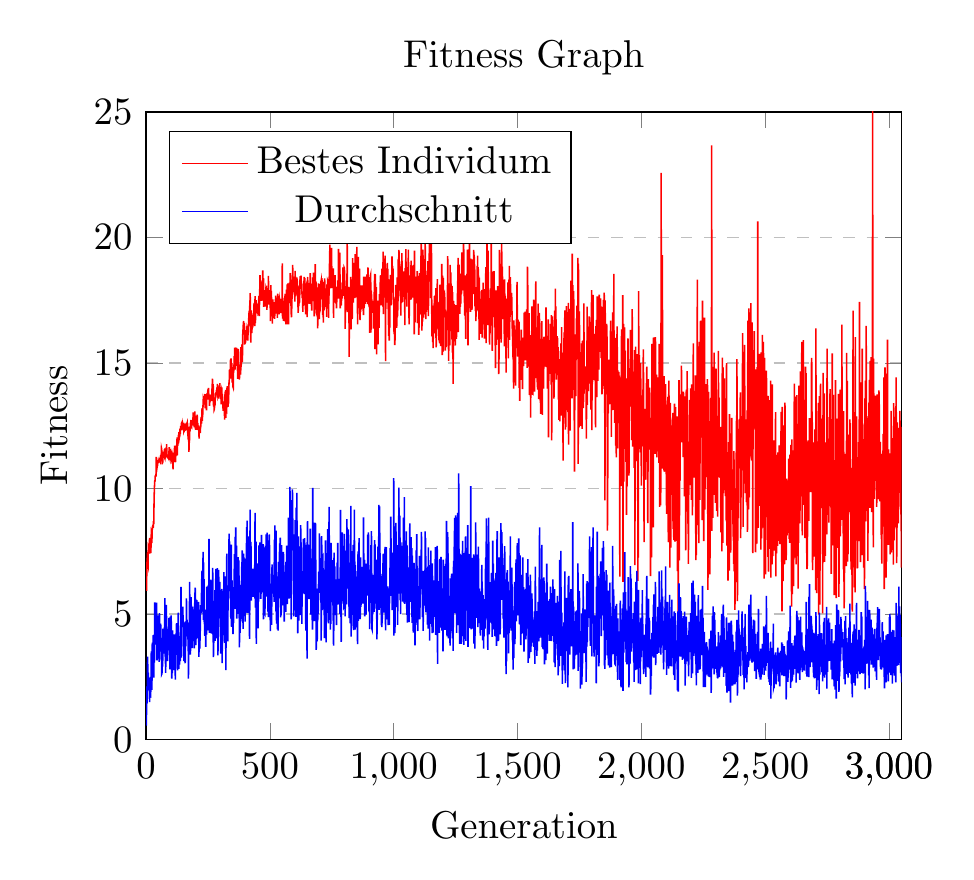
\begin{tikzpicture}[scale=1.4]
\begin{axis}[
    title={Fitness Graph},
    xlabel={Generation},
    ylabel={Fitness},
    xmin=0, xmax=3051,
    ymin=0, ymax=25,
    xtick={0,500,1000,1500,2000,2500,3000,3000},
    ytick={0,5,10,15,20,25},
    legend pos=north west,
    ymajorgrids=true,
    grid style=dashed,
]

\addplot[
    color=red,
    mark=none,
    ]
    coordinates {
	(1,6.896610736846924)(2,5.920971393585205)(3,7.004243850708008)(4,6.99455451965332)(5,7.3171892166137695)(6,7.4652557373046875)(7,6.9916205406188965)(8,6.942554950714111)(9,7.697178840637207)(10,7.666684150695801)(11,7.624490737915039)(12,7.701292991638184)(13,7.600270748138428)(14,8.032538414001465)(15,7.411534309387207)(16,7.6220831871032715)(17,7.500499248504639)(18,7.47577428817749)(19,7.471611022949219)(20,7.721786975860596)(21,8.215011596679688)(22,8.169353485107422)(23,7.824366569519043)(24,8.06535816192627)(25,8.449116706848145)(26,8.479876518249512)(27,8.449116706848145)(28,8.449116706848145)(29,8.457788467407227)(30,8.703351974487305)(31,8.585183143615723)(32,9.3861722946167)(33,9.839818954467773)(34,10.120302200317383)(35,10.303604125976562)(36,10.303604125976562)(37,10.497323036193848)(38,10.497323036193848)(39,10.506497383117676)(40,10.506497383117676)(41,11.256094932556152)(42,11.201187133789062)(43,10.883369445800781)(44,10.833419799804688)(45,10.909629821777344)(46,10.909629821777344)(47,11.00192642211914)(48,11.09583854675293)(49,11.107725143432617)(50,11.095904350280762)(51,11.111742973327637)(52,11.152694702148438)(53,11.114531517028809)(54,11.144309043884277)(55,11.121844291687012)(56,11.104765892028809)(57,11.077836990356445)(58,11.192065238952637)(59,11.298819541931152)(60,11.298819541931152)(61,11.300459861755371)(62,11.612456321716309)(63,11.568941116333008)(64,11.253467559814453)(65,10.961396217346191)(66,11.474258422851562)(67,10.999357223510742)(68,11.26171875)(69,11.34914779663086)(70,11.34914779663086)(71,11.384727478027344)(72,11.34914779663086)(73,11.312761306762695)(74,11.543015480041504)(75,11.55550765991211)(76,11.438035011291504)(77,11.432819366455078)(78,11.307319641113281)(79,11.371990203857422)(80,11.286388397216797)(81,11.404956817626953)(82,11.376131057739258)(83,11.766386032104492)(84,11.266363143920898)(85,11.261539459228516)(86,11.297901153564453)(87,11.261539459228516)(88,11.276586532592773)(89,11.235750198364258)(90,11.214592933654785)(91,11.330151557922363)(92,11.330151557922363)(93,11.616456985473633)(94,11.616456985473633)(95,11.252920150756836)(96,11.208078384399414)(97,11.580755233764648)(98,11.466822624206543)(99,11.394134521484375)(100,11.407119750976562)(101,11.307132720947266)(102,11.414825439453125)(103,11.238789558410645)(104,11.289107322692871)(105,11.38935661315918)(106,11.336462020874023)(107,11.163209915161133)(108,10.91955280303955)(109,10.762274742126465)(110,11.257829666137695)(111,11.430008888244629)(112,11.048759460449219)(113,11.365422248840332)(114,11.223052024841309)(115,11.705148696899414)(116,11.075207710266113)(117,11.433369636535645)(118,11.132770538330078)(119,11.048959732055664)(120,11.409476280212402)(121,11.437257766723633)(122,11.677118301391602)(123,11.713847160339355)(124,11.313216209411621)(125,12.03461742401123)(126,11.32917594909668)(127,11.84760856628418)(128,12.032670021057129)(129,11.96340274810791)(130,12.026735305786133)(131,12.140947341918945)(132,12.024784088134766)(133,12.253138542175293)(134,12.02083683013916)(135,12.082547187805176)(136,12.092849731445312)(137,12.37576961517334)(138,12.171459197998047)(139,12.392931938171387)(140,12.3761568069458)(141,12.435342788696289)(142,12.329865455627441)(143,12.61343002319336)(144,12.512628555297852)(145,12.504156112670898)(146,12.578330993652344)(147,12.499834060668945)(148,12.548742294311523)(149,12.486567497253418)(150,12.523869514465332)(151,12.539960861206055)(152,12.350568771362305)(153,12.402961730957031)(154,12.374781608581543)(155,12.522968292236328)(156,12.53686237335205)(157,12.44105339050293)(158,12.444380760192871)(159,12.438610076904297)(160,12.339167594909668)(161,12.34634017944336)(162,12.399177551269531)(163,12.587322235107422)(164,12.404755592346191)(165,12.59926700592041)(166,12.629351615905762)(167,12.36449146270752)(168,12.245685577392578)(169,12.317340850830078)(170,12.172144889831543)(171,11.941390991210938)(172,12.100804328918457)(173,11.457478523254395)(174,11.87552261352539)(175,11.815727233886719)(176,12.385649681091309)(177,12.371699333190918)(178,12.281112670898438)(179,12.625754356384277)(180,12.388882637023926)(181,12.734683990478516)(182,12.600780487060547)(183,12.546744346618652)(184,12.514751434326172)(185,12.716766357421875)(186,12.52918815612793)(187,12.721278190612793)(188,12.636432647705078)(189,12.605942726135254)(190,13.036943435668945)(191,12.725257873535156)(192,12.683598518371582)(193,12.775470733642578)(194,12.636879920959473)(195,12.58877182006836)(196,12.860732078552246)(197,13.071979522705078)(198,12.65569019317627)(199,12.775884628295898)(200,12.341327667236328)(201,12.574323654174805)(202,12.345996856689453)(203,12.70788288116455)(204,12.336990356445312)(205,12.800787925720215)(206,12.94461727142334)(207,12.849725723266602)(208,12.332534790039062)(209,12.43237018585205)(210,12.462204933166504)(211,12.355692863464355)(212,12.505073547363281)(213,12.302610397338867)(214,11.989819526672363)(215,12.419754981994629)(216,12.26402473449707)(217,12.27830982208252)(218,12.461591720581055)(219,12.206664085388184)(220,12.527235984802246)(221,12.465319633483887)(222,12.851350784301758)(223,12.724289894104004)(224,12.586858749389648)(225,12.836726188659668)(226,13.201416015625)(227,12.69383716583252)(228,12.919742584228516)(229,12.956737518310547)(230,13.36106014251709)(231,13.574910163879395)(232,13.529726028442383)(233,13.677021026611328)(234,13.369956016540527)(235,13.610025405883789)(236,13.646110534667969)(237,13.621960639953613)(238,13.76419448852539)(239,13.198230743408203)(240,13.398150444030762)(241,13.468585014343262)(242,13.46025276184082)(243,13.556068420410156)(244,13.116072654724121)(245,13.639655113220215)(246,13.789071083068848)(247,13.631317138671875)(248,13.549938201904297)(249,13.866223335266113)(250,13.947535514831543)(251,13.537681579589844)(252,14.010560989379883)(253,13.720366477966309)(254,13.726856231689453)(255,13.59577465057373)(256,13.290711402893066)(257,13.42927360534668)(258,13.46855640411377)(259,13.727261543273926)(260,13.607427597045898)(261,13.719259262084961)(262,13.59127426147461)(263,13.752632141113281)(264,13.584237098693848)(265,13.4862642288208)(266,13.93929672241211)(267,14.099616050720215)(268,14.37436294555664)(269,13.952011108398438)(270,13.920929908752441)(271,14.155735969543457)(272,13.353930473327637)(273,13.270903587341309)(274,13.519608497619629)(275,13.146492004394531)(276,13.177186965942383)(277,13.530131340026855)(278,13.290781021118164)(279,13.54223346710205)(280,13.785640716552734)(281,13.598223686218262)(282,13.831284523010254)(283,13.712541580200195)(284,13.930742263793945)(285,13.808953285217285)(286,14.029476165771484)(287,13.86436939239502)(288,14.167061805725098)(289,13.802409172058105)(290,13.682378768920898)(291,13.728797912597656)(292,13.741934776306152)(293,13.818764686584473)(294,13.58059024810791)(295,13.845687866210938)(296,14.116399765014648)(297,13.851978302001953)(298,14.193979263305664)(299,13.707416534423828)(300,13.862805366516113)(301,13.804529190063477)(302,13.85363483428955)(303,13.355101585388184)(304,13.988205909729004)(305,13.441354751586914)(306,14.029687881469727)(307,13.417594909667969)(308,13.771148681640625)(309,13.523871421813965)(310,13.398866653442383)(311,13.0973539352417)(312,13.468505859375)(313,13.386479377746582)(314,13.300848960876465)(315,13.401856422424316)(316,13.28846549987793)(317,12.74088191986084)(318,13.440458297729492)(319,13.856993675231934)(320,13.408331871032715)(321,13.927584648132324)(322,12.819881439208984)(323,13.362794876098633)(324,13.08174991607666)(325,13.06583023071289)(326,13.682670593261719)(327,14.070266723632812)(328,13.407576560974121)(329,14.081904411315918)(330,13.275577545166016)(331,13.280535697937012)(332,13.445354461669922)(333,13.385129928588867)(334,13.894847869873047)(335,14.2554349899292)(336,14.336638450622559)(337,14.749629974365234)(338,14.533491134643555)(339,14.737133026123047)(340,14.375664710998535)(341,15.142931938171387)(342,14.494425773620605)(343,15.186427116394043)(344,14.722400665283203)(345,14.953256607055664)(346,14.957246780395508)(347,14.509247779846191)(348,14.218650817871094)(349,14.659244537353516)(350,14.273990631103516)(351,14.048357009887695)(352,14.017618179321289)(353,14.696419715881348)(354,14.824070930480957)(355,14.804171562194824)(356,15.275089263916016)(357,15.004461288452148)(358,15.607741355895996)(359,14.739222526550293)(360,14.940775871276855)(361,15.577216148376465)(362,15.031641006469727)(363,15.494942665100098)(364,15.582799911499023)(365,15.578255653381348)(366,15.573516845703125)(367,14.882121086120605)(368,15.273076057434082)(369,14.786772727966309)(370,14.370428085327148)(371,14.952892303466797)(372,15.562775611877441)(373,15.501867294311523)(374,14.723614692687988)(375,14.88569450378418)(376,14.816357612609863)(377,14.341215133666992)(378,14.894963264465332)(379,14.887372970581055)(380,14.893570899963379)(381,14.607542991638184)(382,14.542049407958984)(383,15.635055541992188)(384,14.846089363098145)(385,15.284255981445312)(386,15.46042537689209)(387,15.742693901062012)(388,15.035285949707031)(389,15.09117603302002)(390,16.097410202026367)(391,16.234968185424805)(392,16.45393943786621)(393,16.598459243774414)(394,16.670637130737305)(395,16.411758422851562)(396,16.533767700195312)(397,16.54152488708496)(398,15.733420372009277)(399,15.9253511428833)(400,15.903125762939453)(401,16.310699462890625)(402,15.906274795532227)(403,16.110349655151367)(404,16.034774780273438)(405,16.113800048828125)(406,16.46207618713379)(407,16.047557830810547)(408,16.326208114624023)(409,16.270137786865234)(410,15.960972785949707)(411,15.891218185424805)(412,16.398386001586914)(413,16.224775314331055)(414,16.719215393066406)(415,16.84038734436035)(416,17.069629669189453)(417,16.704856872558594)(418,17.281938552856445)(419,16.804697036743164)(420,17.78761100769043)(421,17.47571563720703)(422,16.112764358520508)(423,15.815683364868164)(424,16.618494033813477)(425,17.09554672241211)(426,16.401687622070312)(427,16.19609832763672)(428,16.450380325317383)(429,16.829246520996094)(430,16.40900230407715)(431,16.47278594970703)(432,16.622474670410156)(433,16.970945358276367)(434,16.7656192779541)(435,17.01274299621582)(436,17.39260482788086)(437,16.907045364379883)(438,16.693565368652344)(439,16.470355987548828)(440,17.66329574584961)(441,16.589895248413086)(442,16.762840270996094)(443,17.439239501953125)(444,17.50002670288086)(445,17.041582107543945)(446,17.233854293823242)(447,16.980287551879883)(448,17.251365661621094)(449,17.21235466003418)(450,16.973806381225586)(451,17.157991409301758)(452,16.964820861816406)(453,16.980836868286133)(454,17.398950576782227)(455,17.55830955505371)(456,17.67156219482422)(457,16.86882209777832)(458,17.393253326416016)(459,17.90831756591797)(460,18.50388526916504)(461,18.028963088989258)(462,17.93739128112793)(463,18.117740631103516)(464,17.96273422241211)(465,17.476716995239258)(466,18.2412052154541)(467,17.83285903930664)(468,17.779539108276367)(469,18.287078857421875)(470,17.866811752319336)(471,18.6887264251709)(472,18.061986923217773)(473,18.135995864868164)(474,18.381959915161133)(475,17.237293243408203)(476,17.51453971862793)(477,17.90707778930664)(478,17.45317268371582)(479,17.31186866760254)(480,17.528715133666992)(481,17.5794734954834)(482,17.242326736450195)(483,17.621488571166992)(484,17.931734085083008)(485,17.88146209716797)(486,18.082923889160156)(487,17.341779708862305)(488,17.120285034179688)(489,17.694215774536133)(490,17.64691734313965)(491,17.56205177307129)(492,17.539939880371094)(493,17.570154190063477)(494,18.467941284179688)(495,17.5114688873291)(496,17.32908821105957)(497,17.587783813476562)(498,17.4312801361084)(499,17.90013885498047)(500,17.6003475189209)(501,17.667015075683594)(502,16.664981842041016)(503,17.55928611755371)(504,18.100555419921875)(505,17.100337982177734)(506,17.876325607299805)(507,17.091970443725586)(508,17.07583999633789)(509,17.229759216308594)(510,16.568748474121094)(511,17.336429595947266)(512,17.533706665039062)(513,16.79352378845215)(514,17.04062271118164)(515,17.240440368652344)(516,16.88433074951172)(517,17.42618751525879)(518,17.267396926879883)(519,16.758119583129883)(520,17.026018142700195)(521,17.082704544067383)(522,17.250120162963867)(523,17.681657791137695)(524,17.519264221191406)(525,17.58656120300293)(526,17.23577117919922)(527,16.972881317138672)(528,17.066720962524414)(529,17.54878044128418)(530,16.801347732543945)(531,17.7655029296875)(532,17.57737159729004)(533,17.1651611328125)(534,17.18079376220703)(535,17.54806137084961)(536,17.162410736083984)(537,16.934133529663086)(538,17.332870483398438)(539,17.547773361206055)(540,17.48558807373047)(541,17.32706069946289)(542,17.551042556762695)(543,17.334455490112305)(544,16.98756217956543)(545,17.55402183532715)(546,17.029035568237305)(547,17.4414119720459)(548,17.50503158569336)(549,17.194244384765625)(550,18.970197677612305)(551,16.764379501342773)(552,16.88475799560547)(553,17.073753356933594)(554,17.20667839050293)(555,16.680530548095703)(556,17.33775520324707)(557,16.808732986450195)(558,17.470218658447266)(559,17.586833953857422)(560,16.65488624572754)(561,17.66830825805664)(562,17.755443572998047)(563,17.534069061279297)(564,17.24616813659668)(565,16.540409088134766)(566,17.0947208404541)(567,17.918405532836914)(568,17.741464614868164)(569,16.536766052246094)(570,18.132997512817383)(571,18.002426147460938)(572,17.539030075073242)(573,18.17306900024414)(574,17.46969985961914)(575,16.53662872314453)(576,17.95696449279785)(577,17.655977249145508)(578,17.569843292236328)(579,18.197189331054688)(580,17.9415225982666)(581,17.387781143188477)(582,18.58061981201172)(583,18.525590896606445)(584,17.977840423583984)(585,17.378986358642578)(586,16.990503311157227)(587,16.81953239440918)(588,17.030508041381836)(589,18.324241638183594)(590,17.560335159301758)(591,17.88384437561035)(592,18.905712127685547)(593,18.126867294311523)(594,18.076374053955078)(595,17.9354305267334)(596,17.99142837524414)(597,18.329381942749023)(598,18.441532135009766)(599,18.169748306274414)(600,18.117191314697266)(601,17.443124771118164)(602,18.67343521118164)(603,17.784366607666016)(604,17.660329818725586)(605,18.111665725708008)(606,18.18148422241211)(607,17.896520614624023)(608,17.72356605529785)(609,18.409727096557617)(610,18.203746795654297)(611,18.269939422607422)(612,17.590715408325195)(613,17.48745346069336)(614,17.002046585083008)(615,17.17974853515625)(616,17.801300048828125)(617,17.262149810791016)(618,17.562225341796875)(619,18.092586517333984)(620,17.410348892211914)(621,18.132577896118164)(622,18.428831100463867)(623,18.43535041809082)(624,18.138437271118164)(625,17.95780372619629)(626,18.483476638793945)(627,17.990575790405273)(628,18.15911293029785)(629,18.120359420776367)(630,17.58327865600586)(631,17.76063346862793)(632,17.611360549926758)(633,17.032358169555664)(634,17.4830322265625)(635,17.442142486572266)(636,17.482545852661133)(637,17.74289894104004)(638,18.42851448059082)(639,17.295385360717773)(640,17.740453720092773)(641,18.39300537109375)(642,17.301836013793945)(643,18.117666244506836)(644,16.937496185302734)(645,17.809600830078125)(646,17.65488052368164)(647,17.49299430847168)(648,18.132434844970703)(649,18.1749324798584)(650,16.831127166748047)(651,17.154293060302734)(652,18.422574996948242)(653,18.23552703857422)(654,17.808746337890625)(655,17.5219783782959)(656,17.613082885742188)(657,18.137916564941406)(658,18.1464786529541)(659,17.35247039794922)(660,17.797698974609375)(661,17.95461082458496)(662,17.935632705688477)(663,18.57634735107422)(664,17.729406356811523)(665,17.59747314453125)(666,17.931522369384766)(667,17.388179779052734)(668,17.403108596801758)(669,17.091081619262695)(670,18.006649017333984)(671,18.16149139404297)(672,17.915058135986328)(673,18.409259796142578)(674,17.46232032775879)(675,17.778139114379883)(676,18.600627899169922)(677,17.879838943481445)(678,17.758201599121094)(679,16.859790802001953)(680,17.59970474243164)(681,17.709148406982422)(682,18.040708541870117)(683,18.941438674926758)(684,17.960865020751953)(685,17.288171768188477)(686,18.249643325805664)(687,17.168781280517578)(688,17.00166893005371)(689,16.963029861450195)(690,18.009565353393555)(691,17.72330093383789)(692,17.215044021606445)(693,16.383378982543945)(694,17.389345169067383)(695,17.646657943725586)(696,18.168046951293945)(697,17.083765029907227)(698,17.846824645996094)(699,16.992128372192383)(700,16.743921279907227)(701,18.14590835571289)(702,18.013288497924805)(703,17.05754280090332)(704,17.89238739013672)(705,17.63730812072754)(706,18.236736297607422)(707,18.288759231567383)(708,17.535554885864258)(709,18.18150520324707)(710,18.383378982543945)(711,18.12407112121582)(712,18.23920440673828)(713,16.920654296875)(714,17.840560913085938)(715,17.040498733520508)(716,16.606201171875)(717,18.235227584838867)(718,17.409217834472656)(719,17.09459114074707)(720,17.590137481689453)(721,18.365514755249023)(722,18.170103073120117)(723,17.48783302307129)(724,17.968400955200195)(725,17.581945419311523)(726,17.319746017456055)(727,17.33322525024414)(728,17.733016967773438)(729,16.836292266845703)(730,18.134410858154297)(731,17.825735092163086)(732,17.727558135986328)(733,18.295747756958008)(734,18.271501541137695)(735,17.95366668701172)(736,18.101415634155273)(737,16.794212341308594)(738,17.864255905151367)(739,17.68484878540039)(740,18.703947067260742)(741,18.662473678588867)(742,19.712881088256836)(743,18.738208770751953)(744,18.372426986694336)(745,17.97462272644043)(746,18.722919464111328)(747,18.488609313964844)(748,17.990510940551758)(749,19.587980270385742)(750,18.455381393432617)(751,18.412118911743164)(752,18.45170021057129)(753,17.982345581054688)(754,18.10601806640625)(755,18.21941375732422)(756,18.77083396911621)(757,16.793079376220703)(758,17.678194046020508)(759,17.94451141357422)(760,17.94462013244629)(761,17.51963996887207)(762,18.215917587280273)(763,18.501708984375)(764,17.409393310546875)(765,18.041275024414062)(766,17.402427673339844)(767,17.40300178527832)(768,18.034801483154297)(769,17.180646896362305)(770,17.472354888916016)(771,17.89219093322754)(772,17.629072189331055)(773,17.962848663330078)(774,18.289621353149414)(775,17.59450340270996)(776,17.595548629760742)(777,19.54677391052246)(778,17.917957305908203)(779,18.42707633972168)(780,17.899904251098633)(781,17.848243713378906)(782,19.3923282623291)(783,18.49345588684082)(784,17.174659729003906)(785,18.201662063598633)(786,17.633298873901367)(787,17.847612380981445)(788,17.291534423828125)(789,17.563005447387695)(790,17.551395416259766)(791,17.931568145751953)(792,17.573984146118164)(793,17.679527282714844)(794,18.02524185180664)(795,18.807971954345703)(796,18.266742706298828)(797,18.55715560913086)(798,18.368915557861328)(799,17.671178817749023)(800,18.79518699645996)(801,18.771150588989258)(802,18.168224334716797)(803,18.18299102783203)(804,16.355195999145508)(805,17.82869529724121)(806,17.545089721679688)(807,17.569705963134766)(808,17.643461227416992)(809,17.10116958618164)(810,18.059425354003906)(811,17.139270782470703)(812,20.46389389038086)(813,17.031076431274414)(814,17.907917022705078)(815,17.293588638305664)(816,17.407772064208984)(817,17.705738067626953)(818,18.02889633178711)(819,17.941389083862305)(820,15.248538970947266)(821,17.577363967895508)(822,18.01647186279297)(823,17.63013458251953)(824,17.28062629699707)(825,17.33887481689453)(826,18.42903709411621)(827,17.886754989624023)(828,16.3444881439209)(829,18.193639755249023)(830,17.95839500427246)(831,18.074758529663086)(832,16.74699592590332)(833,16.83186149597168)(834,19.1778621673584)(835,17.68035125732422)(836,18.192890167236328)(837,17.404254913330078)(838,18.434127807617188)(839,18.05166244506836)(840,18.01498031616211)(841,18.988664627075195)(842,18.1341609954834)(843,17.588441848754883)(844,19.337432861328125)(845,18.807310104370117)(846,17.90471076965332)(847,18.770063400268555)(848,18.232820510864258)(849,17.611492156982422)(850,18.708051681518555)(851,19.62554359436035)(852,18.051090240478516)(853,19.093399047851562)(854,16.536596298217773)(855,17.17746925354004)(856,18.042551040649414)(857,19.2263126373291)(858,18.53277587890625)(859,17.45316505432129)(860,18.381675720214844)(861,17.635957717895508)(862,18.761863708496094)(863,17.043010711669922)(864,16.708148956298828)(865,17.79802894592285)(866,17.027441024780273)(867,17.531877517700195)(868,17.297645568847656)(869,17.949684143066406)(870,18.089649200439453)(871,17.956335067749023)(872,18.09125328063965)(873,17.261884689331055)(874,17.2825870513916)(875,17.17685317993164)(876,17.769380569458008)(877,17.08500862121582)(878,16.904075622558594)(879,18.44379234313965)(880,17.190635681152344)(881,17.267887115478516)(882,17.48872184753418)(883,18.01375389099121)(884,17.359384536743164)(885,18.372793197631836)(886,18.093381881713867)(887,18.43771743774414)(888,17.496763229370117)(889,18.128990173339844)(890,18.437538146972656)(891,17.432998657226562)(892,18.525869369506836)(893,18.400480270385742)(894,17.341812133789062)(895,18.158021926879883)(896,18.806550979614258)(897,17.77849769592285)(898,17.781837463378906)(899,18.271997451782227)(900,17.32317352294922)(901,17.231224060058594)(902,18.422931671142578)(903,16.200305938720703)(904,17.823631286621094)(905,16.532888412475586)(906,18.481830596923828)(907,18.523481369018555)(908,16.205984115600586)(909,17.04328155517578)(910,17.882055282592773)(911,16.9930362701416)(912,17.53521156311035)(913,17.179031372070312)(914,17.302928924560547)(915,17.072622299194336)(916,17.409780502319336)(917,17.473718643188477)(918,16.37294578552246)(919,16.958431243896484)(920,16.6685791015625)(921,17.646343231201172)(922,18.027774810791016)(923,18.54929542541504)(924,15.554770469665527)(925,18.53348159790039)(926,18.475568771362305)(927,17.475635528564453)(928,16.897985458374023)(929,17.35509490966797)(930,18.025772094726562)(931,15.343116760253906)(932,16.56534194946289)(933,15.901972770690918)(934,17.30405044555664)(935,17.486164093017578)(936,17.119014739990234)(937,15.743388175964355)(938,17.291872024536133)(939,17.269058227539062)(940,16.62289810180664)(941,16.39790153503418)(942,17.738866806030273)(943,17.60429573059082)(944,17.41463279724121)(945,17.77133560180664)(946,18.40511703491211)(947,18.49362564086914)(948,17.909427642822266)(949,17.292476654052734)(950,17.792102813720703)(951,17.65395164489746)(952,18.756345748901367)(953,18.55228614807129)(954,18.646411895751953)(955,17.961618423461914)(956,17.24530601501465)(957,19.441234588623047)(958,16.943635940551758)(959,18.441810607910156)(960,18.592763900756836)(961,17.60573387145996)(962,18.57741355895996)(963,18.991025924682617)(964,18.320228576660156)(965,19.272762298583984)(966,18.545957565307617)(967,15.073798179626465)(968,18.00469207763672)(969,18.314682006835938)(970,17.81855583190918)(971,18.51441192626953)(972,18.339569091796875)(973,17.406574249267578)(974,18.983823776245117)(975,18.21582794189453)(976,18.753713607788086)(977,18.232463836669922)(978,17.153121948242188)(979,16.527158737182617)(980,16.08197593688965)(981,18.328285217285156)(982,15.892411231994629)(983,17.776752471923828)(984,16.40996742248535)(985,17.511945724487305)(986,18.248170852661133)(987,18.509443283081055)(988,17.58552360534668)(989,17.325061798095703)(990,17.324260711669922)(991,17.839345932006836)(992,18.030668258666992)(993,19.25086784362793)(994,18.657909393310547)(995,18.86896514892578)(996,17.887805938720703)(997,18.75856590270996)(998,18.10013198852539)(999,17.52740478515625)(1000,17.64490509033203)(1001,16.283782958984375)(1002,16.152599334716797)(1003,17.17962074279785)(1004,15.71060562133789)(1005,15.803339958190918)(1006,17.217649459838867)(1007,16.5941104888916)(1008,17.33932113647461)(1009,18.108659744262695)(1010,17.5216064453125)(1011,16.57155990600586)(1012,16.398221969604492)(1013,16.94219207763672)(1014,18.415193557739258)(1015,16.8189754486084)(1016,17.198564529418945)(1017,17.097333908081055)(1018,19.12967872619629)(1019,17.67856788635254)(1020,19.008819580078125)(1021,19.502330780029297)(1022,19.252050399780273)(1023,17.881746292114258)(1024,18.84555435180664)(1025,18.114606857299805)(1026,18.624515533447266)(1027,17.847763061523438)(1028,17.370243072509766)(1029,16.891515731811523)(1030,18.54139518737793)(1031,19.04388999938965)(1032,18.031248092651367)(1033,19.37653160095215)(1034,18.464008331298828)(1035,17.456220626831055)(1036,17.465003967285156)(1037,18.0467529296875)(1038,17.637630462646484)(1039,18.64369773864746)(1040,18.559738159179688)(1041,18.631643295288086)(1042,18.299453735351562)(1043,18.056272506713867)(1044,17.922000885009766)(1045,16.507558822631836)(1046,18.783283233642578)(1047,18.211118698120117)(1048,18.23401641845703)(1049,19.53792381286621)(1050,18.50743293762207)(1051,18.812265396118164)(1052,18.72528076171875)(1053,17.241966247558594)(1054,18.31548309326172)(1055,18.305816650390625)(1056,17.88450813293457)(1057,18.717052459716797)(1058,18.038320541381836)(1059,19.517629623413086)(1060,18.66360092163086)(1061,17.789634704589844)(1062,16.538036346435547)(1063,17.07171058654785)(1064,18.485788345336914)(1065,17.514101028442383)(1066,18.03562355041504)(1067,17.917861938476562)(1068,18.182300567626953)(1069,17.524803161621094)(1070,19.080976486206055)(1071,17.532243728637695)(1072,18.196292877197266)(1073,18.37624740600586)(1074,17.982221603393555)(1075,18.762866973876953)(1076,18.87238311767578)(1077,17.66657829284668)(1078,17.605785369873047)(1079,18.233657836914062)(1080,18.906160354614258)(1081,17.731618881225586)(1082,18.332860946655273)(1083,16.136098861694336)(1084,19.47319221496582)(1085,17.165964126586914)(1086,16.620220184326172)(1087,17.905689239501953)(1088,18.443859100341797)(1089,18.080610275268555)(1090,17.37164306640625)(1091,18.09977149963379)(1092,17.804689407348633)(1093,17.88966178894043)(1094,18.044954299926758)(1095,18.656259536743164)(1096,16.58856201171875)(1097,16.835176467895508)(1098,17.423770904541016)(1099,17.123634338378906)(1100,18.466466903686523)(1101,16.121627807617188)(1102,16.409873962402344)(1103,18.243860244750977)(1104,16.897968292236328)(1105,18.581275939941406)(1106,16.924497604370117)(1107,18.255826950073242)(1108,17.741304397583008)(1109,18.608137130737305)(1110,19.083858489990234)(1111,19.775789260864258)(1112,19.021791458129883)(1113,17.334177017211914)(1114,16.294607162475586)(1115,18.008039474487305)(1116,17.380306243896484)(1117,16.64554786682129)(1118,19.51567268371582)(1119,17.865337371826172)(1120,17.34895896911621)(1121,16.804271697998047)(1122,19.136363983154297)(1123,18.74629020690918)(1124,18.59928321838379)(1125,18.24888038635254)(1126,17.876785278320312)(1127,20.442014694213867)(1128,16.93694496154785)(1129,18.683897018432617)(1130,16.749723434448242)(1131,18.503393173217773)(1132,17.03281593322754)(1133,17.342634201049805)(1134,17.694053649902344)(1135,17.46282196044922)(1136,18.31092643737793)(1137,18.217763900756836)(1138,19.05657386779785)(1139,17.662734985351562)(1140,16.870182037353516)(1141,18.02027130126953)(1142,18.637407302856445)(1143,18.51588249206543)(1144,19.97096061706543)(1145,18.590848922729492)(1146,20.71241569519043)(1147,18.401029586791992)(1148,19.574846267700195)(1149,17.585153579711914)(1150,18.056020736694336)(1151,19.221477508544922)(1152,19.835044860839844)(1153,18.848459243774414)(1154,16.06218147277832)(1155,16.535987854003906)(1156,17.11984634399414)(1157,15.830833435058594)(1158,17.219114303588867)(1159,15.592066764831543)(1160,16.280195236206055)(1161,17.28277015686035)(1162,16.479461669921875)(1163,16.411836624145508)(1164,17.659847259521484)(1165,16.488983154296875)(1166,16.180984497070312)(1167,17.69753074645996)(1168,16.568845748901367)(1169,16.44268226623535)(1170,17.983020782470703)(1171,15.623106956481934)(1172,15.721076011657715)(1173,16.648691177368164)(1174,16.86603546142578)(1175,16.780832290649414)(1176,18.340116500854492)(1177,16.577177047729492)(1178,17.117969512939453)(1179,17.409395217895508)(1180,17.11310577392578)(1181,16.320261001586914)(1182,16.062776565551758)(1183,15.904569625854492)(1184,17.43531608581543)(1185,15.780439376831055)(1186,15.972946166992188)(1187,18.124094009399414)(1188,17.23781394958496)(1189,17.697540283203125)(1190,15.667722702026367)(1191,17.817493438720703)(1192,17.149503707885742)(1193,17.119428634643555)(1194,18.94780731201172)(1195,17.16680908203125)(1196,15.311445236206055)(1197,18.480905532836914)(1198,17.46550941467285)(1199,15.458311080932617)(1200,18.390480041503906)(1201,17.653919219970703)(1202,17.268741607666016)(1203,17.33856773376465)(1204,17.757308959960938)(1205,17.78297233581543)(1206,17.62115478515625)(1207,17.114370346069336)(1208,15.49565601348877)(1209,16.298208236694336)(1210,15.71839714050293)(1211,15.861797332763672)(1212,15.630369186401367)(1213,17.053871154785156)(1214,16.652244567871094)(1215,16.31068229675293)(1216,16.910747528076172)(1217,17.656023025512695)(1218,19.258617401123047)(1219,18.005924224853516)(1220,17.847427368164062)(1221,15.757488250732422)(1222,15.084696769714355)(1223,18.16999626159668)(1224,16.054672241210938)(1225,17.58127784729004)(1226,17.324426651000977)(1227,15.704453468322754)(1228,18.90821647644043)(1229,16.81869888305664)(1230,17.81656265258789)(1231,18.61109733581543)(1232,16.498868942260742)(1233,16.81498908996582)(1234,17.57107925415039)(1235,15.944726943969727)(1236,18.072994232177734)(1237,15.410137176513672)(1238,17.818819046020508)(1239,16.1085205078125)(1240,14.1694917678833)(1241,17.37095069885254)(1242,17.471193313598633)(1243,16.749692916870117)(1244,17.34499740600586)(1245,16.358949661254883)(1246,17.214204788208008)(1247,16.525829315185547)(1248,16.095624923706055)(1249,15.697778701782227)(1250,16.952341079711914)(1251,17.30976104736328)(1252,16.46176528930664)(1253,15.959982872009277)(1254,16.150611877441406)(1255,16.59105682373047)(1256,16.8662109375)(1257,16.853553771972656)(1258,18.236841201782227)(1259,18.303346633911133)(1260,19.185352325439453)(1261,16.22780990600586)(1262,18.669822692871094)(1263,17.822742462158203)(1264,18.921253204345703)(1265,18.269620895385742)(1266,17.22494888305664)(1267,16.953380584716797)(1268,18.313045501708984)(1269,17.232494354248047)(1270,17.83070182800293)(1271,17.3701171875)(1272,18.554759979248047)(1273,17.739219665527344)(1274,17.803857803344727)(1275,19.406600952148438)(1276,18.761817932128906)(1277,18.145668029785156)(1278,17.89775848388672)(1279,18.367027282714844)(1280,18.375755310058594)(1281,19.326316833496094)(1282,19.986648559570312)(1283,19.338228225708008)(1284,17.966928482055664)(1285,17.639896392822266)(1286,17.393024444580078)(1287,16.885929107666016)(1288,18.487571716308594)(1289,18.21127700805664)(1290,16.698535919189453)(1291,15.957511901855469)(1292,18.36859130859375)(1293,17.874879837036133)(1294,17.40974235534668)(1295,18.28990936279297)(1296,18.54629898071289)(1297,17.01820945739746)(1298,19.51806640625)(1299,19.443456649780273)(1300,15.705748558044434)(1301,16.75603485107422)(1302,19.167736053466797)(1303,19.05282211303711)(1304,18.91093635559082)(1305,19.176414489746094)(1306,19.904369354248047)(1307,18.642486572265625)(1308,17.189964294433594)(1309,18.135629653930664)(1310,17.03540802001953)(1311,19.160648345947266)(1312,17.912412643432617)(1313,17.601064682006836)(1314,18.2322940826416)(1315,17.485008239746094)(1316,17.121341705322266)(1317,19.1318359375)(1318,18.627819061279297)(1319,18.830703735351562)(1320,18.699722290039062)(1321,17.745973587036133)(1322,18.547588348388672)(1323,19.509572982788086)(1324,18.702878952026367)(1325,19.30658531188965)(1326,18.604957580566406)(1327,18.930387496948242)(1328,17.26604652404785)(1329,17.352508544921875)(1330,17.066781997680664)(1331,17.308656692504883)(1332,16.665498733520508)(1333,17.739299774169922)(1334,17.043777465820312)(1335,18.025348663330078)(1336,17.06598472595215)(1337,18.869962692260742)(1338,17.859704971313477)(1339,19.278013229370117)(1340,17.11441421508789)(1341,18.81356430053711)(1342,18.567697525024414)(1343,18.246549606323242)(1344,17.530681610107422)(1345,15.923298835754395)(1346,18.39605140686035)(1347,16.681108474731445)(1348,16.594697952270508)(1349,17.310468673706055)(1350,16.1574649810791)(1351,16.378894805908203)(1352,17.455141067504883)(1353,16.455909729003906)(1354,17.251100540161133)(1355,17.76387596130371)(1356,17.91168975830078)(1357,16.007465362548828)(1358,17.286468505859375)(1359,16.902441024780273)(1360,17.169464111328125)(1361,18.19655418395996)(1362,17.094615936279297)(1363,17.053918838500977)(1364,17.939674377441406)(1365,17.116785049438477)(1366,15.974668502807617)(1367,17.772510528564453)(1368,17.575389862060547)(1369,17.117521286010742)(1370,17.37629508972168)(1371,17.823205947875977)(1372,18.82231903076172)(1373,15.794529914855957)(1374,17.246543884277344)(1375,17.096113204956055)(1376,19.181236267089844)(1377,20.27115821838379)(1378,18.572542190551758)(1379,16.81955337524414)(1380,16.507333755493164)(1381,19.4724178314209)(1382,18.157655715942383)(1383,17.870248794555664)(1384,17.431257247924805)(1385,16.873252868652344)(1386,16.670127868652344)(1387,15.734734535217285)(1388,16.317068099975586)(1389,16.203916549682617)(1390,16.605205535888672)(1391,16.957942962646484)(1392,17.976531982421875)(1393,16.85081672668457)(1394,20.48255157470703)(1395,17.208984375)(1396,18.196456909179688)(1397,16.50918197631836)(1398,15.4869966506958)(1399,18.64400863647461)(1400,18.37197494506836)(1401,17.737085342407227)(1402,17.881322860717773)(1403,16.82566261291504)(1404,18.275882720947266)(1405,18.662336349487305)(1406,17.864994049072266)(1407,17.431598663330078)(1408,16.422454833984375)(1409,17.694477081298828)(1410,15.815741539001465)(1411,14.796163558959961)(1412,16.818828582763672)(1413,17.89337921142578)(1414,15.72538948059082)(1415,16.246055603027344)(1416,15.929676055908203)(1417,16.97348403930664)(1418,17.06047821044922)(1419,17.192705154418945)(1420,18.066259384155273)(1421,17.17508888244629)(1422,17.48954963684082)(1423,16.949573516845703)(1424,14.561742782592773)(1425,15.075654029846191)(1426,16.284381866455078)(1427,19.501686096191406)(1428,18.079008102416992)(1429,18.7606258392334)(1430,15.964054107666016)(1431,18.945858001708984)(1432,18.30729103088379)(1433,18.63629722595215)(1434,15.811838150024414)(1435,16.809221267700195)(1436,19.853086471557617)(1437,17.270198822021484)(1438,17.29966163635254)(1439,18.83534049987793)(1440,16.745214462280273)(1441,16.99994468688965)(1442,18.190059661865234)(1443,16.951242446899414)(1444,17.78291893005371)(1445,18.31499671936035)(1446,16.590871810913086)(1447,15.65995979309082)(1448,18.335336685180664)(1449,16.275531768798828)(1450,17.676496505737305)(1451,17.361433029174805)(1452,16.286619186401367)(1453,15.825398445129395)(1454,14.613356590270996)(1455,17.556907653808594)(1456,16.267778396606445)(1457,17.034894943237305)(1458,16.43804168701172)(1459,16.232114791870117)(1460,16.90883445739746)(1461,18.21073341369629)(1462,17.34109115600586)(1463,15.184423446655273)(1464,17.979402542114258)(1465,18.31913948059082)(1466,16.75747299194336)(1467,18.873680114746094)(1468,15.91658878326416)(1469,17.452890396118164)(1470,16.83481788635254)(1471,18.423559188842773)(1472,17.862529754638672)(1473,17.209686279296875)(1474,16.96710968017578)(1475,17.03078842163086)(1476,17.795927047729492)(1477,17.48017692565918)(1478,16.742202758789062)(1479,16.253477096557617)(1480,15.999582290649414)(1481,15.564518928527832)(1482,15.147003173828125)(1483,15.32008171081543)(1484,13.980080604553223)(1485,16.7008113861084)(1486,16.38112449645996)(1487,15.195009231567383)(1488,15.49087905883789)(1489,15.328588485717773)(1490,14.925463676452637)(1491,15.301995277404785)(1492,14.10077953338623)(1493,16.241533279418945)(1494,16.335166931152344)(1495,16.50080108642578)(1496,16.75613784790039)(1497,15.861920356750488)(1498,18.232927322387695)(1499,17.03151512145996)(1500,15.808440208435059)(1501,15.25087833404541)(1502,16.728893280029297)(1503,16.106462478637695)(1504,15.839588165283203)(1505,15.561720848083496)(1506,16.650131225585938)(1507,14.01351547241211)(1508,15.89306640625)(1509,13.48766040802002)(1510,15.462831497192383)(1511,15.714695930480957)(1512,14.334249496459961)(1513,14.492754936218262)(1514,15.400757789611816)(1515,16.327056884765625)(1516,15.856392860412598)(1517,15.397785186767578)(1518,14.507230758666992)(1519,15.341203689575195)(1520,13.962470054626465)(1521,15.101656913757324)(1522,16.008726119995117)(1523,15.379005432128906)(1524,14.880403518676758)(1525,15.12635612487793)(1526,15.164862632751465)(1527,17.010421752929688)(1528,15.616095542907715)(1529,16.333829879760742)(1530,15.917522430419922)(1531,17.04840850830078)(1532,15.104162216186523)(1533,15.950316429138184)(1534,16.13345718383789)(1535,15.181187629699707)(1536,16.423965454101562)(1537,17.1401309967041)(1538,15.863286018371582)(1539,14.802478790283203)(1540,18.835371017456055)(1541,18.64145278930664)(1542,15.252758026123047)(1543,14.860902786254883)(1544,15.976715087890625)(1545,16.94204330444336)(1546,15.833353996276855)(1547,16.988306045532227)(1548,13.727374076843262)(1549,15.4297513961792)(1550,15.11625862121582)(1551,16.113513946533203)(1552,14.401131629943848)(1553,12.82667064666748)(1554,15.677597999572754)(1555,15.210691452026367)(1556,15.65297794342041)(1557,14.211874961853027)(1558,17.253026962280273)(1559,14.781416893005371)(1560,16.180845260620117)(1561,13.761462211608887)(1562,13.75529670715332)(1563,17.04637336730957)(1564,16.576101303100586)(1565,17.518938064575195)(1566,17.446731567382812)(1567,14.810110092163086)(1568,16.98430061340332)(1569,13.8577299118042)(1570,15.766066551208496)(1571,16.55983543395996)(1572,15.44575023651123)(1573,17.974361419677734)(1574,18.25533676147461)(1575,14.399514198303223)(1576,16.320995330810547)(1577,15.577948570251465)(1578,14.804969787597656)(1579,14.239361763000488)(1580,14.320306777954102)(1581,13.935927391052246)(1582,15.405702590942383)(1583,17.362003326416016)(1584,15.317452430725098)(1585,13.559205055236816)(1586,16.172073364257812)(1587,15.248995780944824)(1588,16.99468421936035)(1589,16.606977462768555)(1590,14.335453033447266)(1591,13.516355514526367)(1592,15.861201286315918)(1593,12.972865104675293)(1594,15.485054969787598)(1595,15.618886947631836)(1596,15.358638763427734)(1597,16.032800674438477)(1598,16.667476654052734)(1599,14.051575660705566)(1600,12.932698249816895)(1601,15.672415733337402)(1602,15.959142684936523)(1603,15.263527870178223)(1604,15.407583236694336)(1605,13.983331680297852)(1606,15.013144493103027)(1607,16.04802131652832)(1608,15.608404159545898)(1609,15.052087783813477)(1610,15.83161449432373)(1611,15.869022369384766)(1612,15.198169708251953)(1613,14.854353904724121)(1614,15.62369155883789)(1615,17.211400985717773)(1616,15.74549674987793)(1617,14.84032154083252)(1618,15.061203956604004)(1619,16.082366943359375)(1620,15.675628662109375)(1621,13.975878715515137)(1622,14.591682434082031)(1623,14.580146789550781)(1624,16.733354568481445)(1625,12.035429000854492)(1626,14.364643096923828)(1627,14.789082527160645)(1628,15.912562370300293)(1629,15.074233055114746)(1630,14.681528091430664)(1631,14.668607711791992)(1632,14.566630363464355)(1633,16.557762145996094)(1634,15.020561218261719)(1635,16.279356002807617)(1636,14.142388343811035)(1637,16.905752182006836)(1638,11.918410301208496)(1639,15.797256469726562)(1640,15.872124671936035)(1641,16.853702545166016)(1642,15.543771743774414)(1643,14.24233627319336)(1644,16.20958709716797)(1645,16.447877883911133)(1646,14.602547645568848)(1647,13.586426734924316)(1648,13.96826171875)(1649,15.473028182983398)(1650,17.089763641357422)(1651,16.198396682739258)(1652,15.552793502807617)(1653,17.958782196044922)(1654,14.58398723602295)(1655,17.251832962036133)(1656,15.122873306274414)(1657,14.3391752243042)(1658,15.198495864868164)(1659,14.96870231628418)(1660,16.06914710998535)(1661,15.106300354003906)(1662,15.99878978729248)(1663,14.729757308959961)(1664,15.629817962646484)(1665,13.53751277923584)(1666,15.468422889709473)(1667,12.734256744384766)(1668,15.156354904174805)(1669,13.168729782104492)(1670,14.152386665344238)(1671,12.670900344848633)(1672,14.748708724975586)(1673,14.813228607177734)(1674,13.850711822509766)(1675,15.784067153930664)(1676,12.903223991394043)(1677,13.471226692199707)(1678,16.429229736328125)(1679,14.259753227233887)(1680,14.648544311523438)(1681,14.200986862182617)(1682,14.87718391418457)(1683,13.590581893920898)(1684,11.112940788269043)(1685,14.387308120727539)(1686,15.403675079345703)(1687,15.274208068847656)(1688,16.223207473754883)(1689,14.502394676208496)(1690,15.785848617553711)(1691,17.096620559692383)(1692,13.522253036499023)(1693,12.348994255065918)(1694,12.786384582519531)(1695,12.738972663879395)(1696,14.557389259338379)(1697,17.26839828491211)(1698,13.56398868560791)(1699,13.492507934570312)(1700,15.077383041381836)(1701,13.265632629394531)(1702,13.562614440917969)(1703,13.076769828796387)(1704,13.07345962524414)(1705,17.396913528442383)(1706,11.745465278625488)(1707,16.943233489990234)(1708,14.724194526672363)(1709,13.464384078979492)(1710,16.555360794067383)(1711,17.156681060791016)(1712,12.303178787231445)(1713,16.86115074157715)(1714,16.828960418701172)(1715,17.0650634765625)(1716,18.27630043029785)(1717,16.273279190063477)(1718,18.17293357849121)(1719,16.17950439453125)(1720,13.58663272857666)(1721,19.353321075439453)(1722,17.022872924804688)(1723,18.096349716186523)(1724,17.808792114257812)(1725,13.928763389587402)(1726,17.859943389892578)(1727,17.510692596435547)(1728,14.148918151855469)(1729,13.063000679016113)(1730,10.673580169677734)(1731,13.222885131835938)(1732,15.913124084472656)(1733,16.139341354370117)(1734,15.97036075592041)(1735,13.679708480834961)(1736,15.116113662719727)(1737,15.384279251098633)(1738,16.7740421295166)(1739,15.884565353393555)(1740,17.28748893737793)(1741,16.424224853515625)(1742,15.97080135345459)(1743,15.150177001953125)(1744,19.18729019165039)(1745,10.98363208770752)(1746,18.96121597290039)(1747,16.646053314208984)(1748,15.487069129943848)(1749,12.434381484985352)(1750,17.053497314453125)(1751,13.31214714050293)(1752,13.70571231842041)(1753,15.429085731506348)(1754,14.972946166992188)(1755,12.492060661315918)(1756,12.601439476013184)(1757,14.358601570129395)(1758,13.585535049438477)(1759,15.783745765686035)(1760,12.776103019714355)(1761,12.377349853515625)(1762,15.880642890930176)(1763,13.799867630004883)(1764,14.7852783203125)(1765,15.899660110473633)(1766,13.204144477844238)(1767,14.038007736206055)(1768,17.372623443603516)(1769,13.783380508422852)(1770,14.296184539794922)(1771,13.950775146484375)(1772,14.530111312866211)(1773,14.864837646484375)(1774,14.601523399353027)(1775,14.59156608581543)(1776,14.192497253417969)(1777,13.902613639831543)(1778,11.990684509277344)(1779,13.879977226257324)(1780,13.55456829071045)(1781,17.246320724487305)(1782,13.334460258483887)(1783,14.777503967285156)(1784,14.347466468811035)(1785,16.44718360900879)(1786,13.87827205657959)(1787,15.237237930297852)(1788,14.525243759155273)(1789,16.85361099243164)(1790,14.177241325378418)(1791,16.637348175048828)(1792,15.865472793579102)(1793,15.34805965423584)(1794,15.41280746459961)(1795,14.44144058227539)(1796,13.145256996154785)(1797,16.816499710083008)(1798,15.417481422424316)(1799,17.899169921875)(1800,12.325292587280273)(1801,14.225688934326172)(1802,14.217422485351562)(1803,14.785877227783203)(1804,15.621744155883789)(1805,17.71253204345703)(1806,14.327007293701172)(1807,15.720187187194824)(1808,16.1618595123291)(1809,14.881410598754883)(1810,15.851725578308105)(1811,14.51401424407959)(1812,14.555150985717773)(1813,15.80169677734375)(1814,15.443397521972656)(1815,12.435770988464355)(1816,16.464353561401367)(1817,14.004314422607422)(1818,13.697725296020508)(1819,16.71480941772461)(1820,13.638277053833008)(1821,16.243553161621094)(1822,17.65595054626465)(1823,14.759481430053711)(1824,14.291635513305664)(1825,16.05620765686035)(1826,15.778265953063965)(1827,17.070682525634766)(1828,14.733806610107422)(1829,16.637786865234375)(1830,17.720840454101562)(1831,17.363977432250977)(1832,16.778913497924805)(1833,15.446606636047363)(1834,15.700691223144531)(1835,17.57248878479004)(1836,17.25405502319336)(1837,15.596183776855469)(1838,15.199644088745117)(1839,17.239355087280273)(1840,16.73681640625)(1841,13.75562572479248)(1842,15.602788925170898)(1843,15.582375526428223)(1844,13.970858573913574)(1845,17.22714614868164)(1846,16.209854125976562)(1847,17.511930465698242)(1848,15.329092025756836)(1849,15.11087417602539)(1850,17.80052947998047)(1851,16.784536361694336)(1852,14.596077919006348)(1853,9.52491283416748)(1854,17.492528915405273)(1855,13.748104095458984)(1856,15.027031898498535)(1857,14.634818077087402)(1858,15.625753402709961)(1859,13.816683769226074)(1860,16.562782287597656)(1861,16.23455047607422)(1862,15.333593368530273)(1863,8.326824188232422)(1864,9.263449668884277)(1865,14.30173110961914)(1866,14.80307674407959)(1867,12.995856285095215)(1868,14.332908630371094)(1869,15.135685920715332)(1870,13.520207405090332)(1871,13.729986190795898)(1872,13.754745483398438)(1873,14.70008373260498)(1874,13.363677024841309)(1875,15.846441268920898)(1876,16.683687210083008)(1877,14.394912719726562)(1878,15.294600486755371)(1879,12.055152893066406)(1880,14.871968269348145)(1881,15.478487968444824)(1882,15.885628700256348)(1883,15.068920135498047)(1884,17.01413917541504)(1885,13.456332206726074)(1886,13.133979797363281)(1887,16.95907974243164)(1888,16.03754997253418)(1889,18.546009063720703)(1890,13.746158599853516)(1891,15.006202697753906)(1892,12.617546081542969)(1893,15.225003242492676)(1894,13.145966529846191)(1895,15.39385986328125)(1896,11.704728126525879)(1897,15.99754810333252)(1898,11.899333953857422)(1899,11.238543510437012)(1900,14.983834266662598)(1901,15.03126335144043)(1902,16.455211639404297)(1903,15.061630249023438)(1904,11.5958890914917)(1905,14.707111358642578)(1906,12.860306739807129)(1907,13.578102111816406)(1908,12.604606628417969)(1909,14.645773887634277)(1910,14.191422462463379)(1911,14.498685836791992)(1912,14.393340110778809)(1913,6.495210647583008)(1914,13.213603973388672)(1915,13.097195625305176)(1916,11.640595436096191)(1917,10.300514221191406)(1918,10.253378868103027)(1919,10.101263999938965)(1920,16.33720588684082)(1921,13.513439178466797)(1922,14.55647087097168)(1923,14.999707221984863)(1924,14.792440414428711)(1925,17.703462600708008)(1926,6.286880016326904)(1927,16.069936752319336)(1928,16.55997085571289)(1929,10.279569625854492)(1930,13.5911283493042)(1931,13.509020805358887)(1932,16.420652389526367)(1933,15.107068061828613)(1934,11.575729370117188)(1935,15.493474960327148)(1936,13.830982208251953)(1937,14.014409065246582)(1938,11.062938690185547)(1939,14.123370170593262)(1940,8.950811386108398)(1941,14.391130447387695)(1942,10.084308624267578)(1943,12.991434097290039)(1944,13.706085205078125)(1945,13.662242889404297)(1946,15.98529052734375)(1947,11.174812316894531)(1948,12.894157409667969)(1949,14.028398513793945)(1950,10.51901626586914)(1951,12.643580436706543)(1952,13.550518989562988)(1953,14.795990943908691)(1954,14.445956230163574)(1955,14.66532039642334)(1956,16.321073532104492)(1957,15.558255195617676)(1958,13.25976848602295)(1959,13.862434387207031)(1960,16.214279174804688)(1961,11.932369232177734)(1962,15.82183837890625)(1963,17.146032333374023)(1964,15.301600456237793)(1965,11.668898582458496)(1966,13.210379600524902)(1967,13.659961700439453)(1968,13.489776611328125)(1969,13.663936614990234)(1970,13.719950675964355)(1971,10.8230619430542)(1972,14.799553871154785)(1973,15.508286476135254)(1974,6.953574180603027)(1975,13.321967124938965)(1976,13.949235916137695)(1977,15.657106399536133)(1978,13.169548034667969)(1979,11.087400436401367)(1980,11.950281143188477)(1981,13.791601181030273)(1982,14.721392631530762)(1983,11.920682907104492)(1984,15.356371879577637)(1985,13.901490211486816)(1986,6.321865081787109)(1987,15.146581649780273)(1988,7.243292808532715)(1989,17.862796783447266)(1990,14.51883316040039)(1991,14.420161247253418)(1992,15.312773704528809)(1993,12.58939266204834)(1994,13.019312858581543)(1995,14.335362434387207)(1996,11.436583518981934)(1997,14.99277400970459)(1998,13.752540588378906)(1999,12.877398490905762)(2000,10.113286972045898)(2001,10.833298683166504)(2002,13.70793342590332)(2003,13.614378929138184)(2004,13.050128936767578)(2005,11.681802749633789)(2006,13.675542831420898)(2007,14.014913558959961)(2008,15.545912742614746)(2009,14.014565467834473)(2010,12.43839168548584)(2011,7.867124080657959)(2012,11.840251922607422)(2013,10.343457221984863)(2014,13.16835880279541)(2015,12.989051818847656)(2016,11.856776237487793)(2017,10.356828689575195)(2018,12.21264362335205)(2019,11.061064720153809)(2020,12.908236503601074)(2021,14.315961837768555)(2022,14.855956077575684)(2023,13.667082786560059)(2024,12.951395034790039)(2025,11.582005500793457)(2026,8.619353294372559)(2027,11.273820877075195)(2028,14.353947639465332)(2029,13.353752136230469)(2030,11.554306030273438)(2031,12.065241813659668)(2032,12.852507591247559)(2033,14.016328811645508)(2034,12.509533882141113)(2035,12.7426118850708)(2036,12.001614570617676)(2037,6.516263484954834)(2038,12.81480884552002)(2039,9.660470962524414)(2040,11.018036842346191)(2041,7.256417274475098)(2042,13.556361198425293)(2043,15.765213012695312)(2044,8.45659065246582)(2045,12.490110397338867)(2046,10.440322875976562)(2047,11.449784278869629)(2048,8.4503812789917)(2049,16.008346557617188)(2050,13.443573951721191)(2051,13.4364652633667)(2052,16.025659561157227)(2053,14.738560676574707)(2054,13.638813972473145)(2055,13.241498947143555)(2056,11.38031005859375)(2057,16.034486770629883)(2058,13.037237167358398)(2059,12.657633781433105)(2060,13.900193214416504)(2061,13.573349952697754)(2062,14.541749000549316)(2063,11.245881080627441)(2064,13.250475883483887)(2065,12.681428909301758)(2066,14.431221961975098)(2067,13.669364929199219)(2068,11.633793830871582)(2069,14.412433624267578)(2070,12.801666259765625)(2071,11.021943092346191)(2072,15.763282775878906)(2073,13.618902206420898)(2074,9.266268730163574)(2075,12.744470596313477)(2076,14.897647857666016)(2077,9.989130020141602)(2078,9.33178424835205)(2079,11.25252914428711)(2080,22.575008392333984)(2081,14.574921607971191)(2082,11.246408462524414)(2083,10.795214653015137)(2084,13.06373119354248)(2085,19.293642044067383)(2086,12.68932819366455)(2087,10.796385765075684)(2088,12.473831176757812)(2089,12.454833030700684)(2090,12.741568565368652)(2091,10.722834587097168)(2092,14.475892066955566)(2093,10.701252937316895)(2094,10.704812049865723)(2095,12.742086410522461)(2096,12.848531723022461)(2097,11.089910507202148)(2098,14.160810470581055)(2099,12.710819244384766)(2100,11.679430961608887)(2101,10.041949272155762)(2102,8.991848945617676)(2103,9.731461524963379)(2104,12.852499961853027)(2105,13.34566593170166)(2106,11.181745529174805)(2107,13.652817726135254)(2108,9.44493579864502)(2109,7.8657307624816895)(2110,12.002129554748535)(2111,14.302289962768555)(2112,13.2605619430542)(2113,10.849922180175781)(2114,12.056236267089844)(2115,6.844902992248535)(2116,12.72775650024414)(2117,13.414436340332031)(2118,9.899568557739258)(2119,7.645036220550537)(2120,10.854853630065918)(2121,10.710238456726074)(2122,12.511045455932617)(2123,10.971399307250977)(2124,9.961555480957031)(2125,12.74136734008789)(2126,10.53175163269043)(2127,13.013096809387207)(2128,8.392882347106934)(2129,9.923779487609863)(2130,10.746216773986816)(2131,7.949191570281982)(2132,12.376258850097656)(2133,11.480132102966309)(2134,13.386527061462402)(2135,8.347880363464355)(2136,7.888033866882324)(2137,12.98295783996582)(2138,13.237874031066895)(2139,11.502660751342773)(2140,9.533679962158203)(2141,7.9122185707092285)(2142,11.99731731414795)(2143,10.07422161102295)(2144,11.995630264282227)(2145,12.87557315826416)(2146,6.707098484039307)(2147,12.2024507522583)(2148,8.764589309692383)(2149,4.769046306610107)(2150,10.91401195526123)(2151,9.673970222473145)(2152,14.319091796875)(2153,7.137584209442139)(2154,8.965509414672852)(2155,11.268068313598633)(2156,10.316106796264648)(2157,13.749861717224121)(2158,12.757521629333496)(2159,12.405081748962402)(2160,13.27653980255127)(2161,12.939388275146484)(2162,14.891304016113281)(2163,11.841405868530273)(2164,12.43212890625)(2165,11.879608154296875)(2166,12.636680603027344)(2167,12.279824256896973)(2168,12.598699569702148)(2169,11.249028205871582)(2170,13.860359191894531)(2171,13.376273155212402)(2172,13.5420560836792)(2173,13.264694213867188)(2174,9.688613891601562)(2175,13.673572540283203)(2176,12.18127155303955)(2177,11.802791595458984)(2178,12.81660270690918)(2179,7.540347576141357)(2180,7.669098854064941)(2181,13.797201156616211)(2182,13.933370590209961)(2183,12.43804931640625)(2184,9.480189323425293)(2185,14.680941581726074)(2186,12.25521469116211)(2187,10.727190971374512)(2188,8.60490608215332)(2189,9.484763145446777)(2190,6.997071743011475)(2191,8.719653129577637)(2192,11.787040710449219)(2193,11.473040580749512)(2194,12.185340881347656)(2195,13.516622543334961)(2196,10.988065719604492)(2197,13.526535987854004)(2198,10.137133598327637)(2199,13.986406326293945)(2200,13.178205490112305)(2201,13.860051155090332)(2202,9.549829483032227)(2203,14.145767211914062)(2204,14.055798530578613)(2205,13.057541847229004)(2206,8.926570892333984)(2207,9.658990859985352)(2208,12.8939847946167)(2209,14.259848594665527)(2210,15.777933120727539)(2211,11.54293155670166)(2212,10.435199737548828)(2213,11.507956504821777)(2214,12.879169464111328)(2215,11.861063957214355)(2216,13.887622833251953)(2217,11.336852073669434)(2218,14.506330490112305)(2219,12.565184593200684)(2220,7.151656627655029)(2221,9.324790000915527)(2222,7.352583408355713)(2223,11.792043685913086)(2224,12.656758308410645)(2225,10.421019554138184)(2226,18.318880081176758)(2227,11.606151580810547)(2228,13.716259002685547)(2229,8.543403625488281)(2230,11.483201026916504)(2231,12.187155723571777)(2232,7.8267035484313965)(2233,12.79568099975586)(2234,15.846151351928711)(2235,11.626248359680176)(2236,9.544259071350098)(2237,11.445032119750977)(2238,13.746600151062012)(2239,16.690399169921875)(2240,13.347296714782715)(2241,12.71298599243164)(2242,12.031332015991211)(2243,13.547749519348145)(2244,13.964941024780273)(2245,16.51028823852539)(2246,8.746365547180176)(2247,17.48037338256836)(2248,10.662243843078613)(2249,12.998143196105957)(2250,12.00312328338623)(2251,8.892523765563965)(2252,7.90701150894165)(2253,9.936270713806152)(2254,11.42795467376709)(2255,16.804981231689453)(2256,9.160477638244629)(2257,13.797627449035645)(2258,9.99656867980957)(2259,14.158125877380371)(2260,11.736363410949707)(2261,11.124178886413574)(2262,10.648035049438477)(2263,12.375385284423828)(2264,13.094053268432617)(2265,13.740303039550781)(2266,10.455549240112305)(2267,14.354619979858398)(2268,10.084568977355957)(2269,5.96515417098999)(2270,12.492140769958496)(2271,7.68700647354126)(2272,13.851583480834961)(2273,11.22721004486084)(2274,10.576194763183594)(2275,10.821748733520508)(2276,8.506135940551758)(2277,6.5820183753967285)(2278,10.866869926452637)(2279,10.840006828308105)(2280,12.106352806091309)(2281,13.613381385803223)(2282,10.653498649597168)(2283,12.748923301696777)(2284,23.668546676635742)(2285,8.313148498535156)(2286,13.489060401916504)(2287,14.433490753173828)(2288,14.40106201171875)(2289,8.833111763000488)(2290,13.930163383483887)(2291,14.84831428527832)(2292,11.69173812866211)(2293,12.067376136779785)(2294,15.417595863342285)(2295,13.548093795776367)(2296,9.748933792114258)(2297,12.534034729003906)(2298,12.558830261230469)(2299,9.429671287536621)(2300,11.5944185256958)(2301,12.29692268371582)(2302,14.773453712463379)(2303,9.974761962890625)(2304,9.11120319366455)(2305,10.177760124206543)(2306,9.643575668334961)(2307,12.025925636291504)(2308,8.881954193115234)(2309,12.387571334838867)(2310,10.826701164245605)(2311,15.48635482788086)(2312,12.824991226196289)(2313,11.658834457397461)(2314,13.622543334960938)(2315,11.039523124694824)(2316,10.465850830078125)(2317,10.4585599899292)(2318,12.395258903503418)(2319,11.476367950439453)(2320,12.454618453979492)(2321,8.250539779663086)(2322,10.347061157226562)(2323,11.233542442321777)(2324,11.772674560546875)(2325,7.499231338500977)(2326,11.663270950317383)(2327,15.21766185760498)(2328,12.178912162780762)(2329,7.835810661315918)(2330,14.82175350189209)(2331,9.81928825378418)(2332,11.230188369750977)(2333,14.351191520690918)(2334,12.578940391540527)(2335,14.38906478881836)(2336,10.357268333435059)(2337,10.462075233459473)(2338,13.588813781738281)(2339,9.694401741027832)(2340,11.675965309143066)(2341,10.696409225463867)(2342,11.330008506774902)(2343,8.6895112991333)(2344,14.999332427978516)(2345,10.526408195495605)(2346,7.730041027069092)(2347,8.350652694702148)(2348,8.767376899719238)(2349,10.898797035217285)(2350,6.332857608795166)(2351,8.863887786865234)(2352,9.005237579345703)(2353,11.847482681274414)(2354,10.933979034423828)(2355,6.7303996086120605)(2356,12.959893226623535)(2357,9.823643684387207)(2358,9.166728019714355)(2359,8.141281127929688)(2360,7.452330589294434)(2361,7.5498738288879395)(2362,11.451358795166016)(2363,9.850940704345703)(2364,12.062752723693848)(2365,12.810303688049316)(2366,9.151609420776367)(2367,10.760610580444336)(2368,9.91836929321289)(2369,9.950435638427734)(2370,8.697535514831543)(2371,8.203986167907715)(2372,8.252737998962402)(2373,6.994556903839111)(2374,11.492921829223633)(2375,6.6961164474487305)(2376,7.080205917358398)(2377,7.8288493156433105)(2378,5.168750286102295)(2379,7.21837043762207)(2380,10.011016845703125)(2381,6.275956630706787)(2382,6.391942977905273)(2383,10.727622985839844)(2384,12.695201873779297)(2385,11.551570892333984)(2386,15.156180381774902)(2387,11.464977264404297)(2388,5.513301849365234)(2389,6.694655418395996)(2390,12.376482009887695)(2391,10.995647430419922)(2392,8.82091999053955)(2393,11.300849914550781)(2394,11.822917938232422)(2395,12.744840621948242)(2396,12.054956436157227)(2397,12.769868850708008)(2398,10.971163749694824)(2399,13.399657249450684)(2400,13.831372261047363)(2401,8.029311180114746)(2402,9.110211372375488)(2403,10.690528869628906)(2404,11.494089126586914)(2405,10.88785171508789)(2406,12.884316444396973)(2407,12.239134788513184)(2408,13.171388626098633)(2409,16.192848205566406)(2410,14.364118576049805)(2411,8.472589492797852)(2412,11.058362007141113)(2413,12.533607482910156)(2414,10.807160377502441)(2415,11.229466438293457)(2416,13.216621398925781)(2417,15.723875045776367)(2418,12.342462539672852)(2419,11.102251052856445)(2420,9.814716339111328)(2421,10.366663932800293)(2422,12.755165100097656)(2423,12.246578216552734)(2424,9.455554962158203)(2425,12.145071029663086)(2426,10.606812477111816)(2427,13.111427307128906)(2428,8.27489948272705)(2429,8.421749114990234)(2430,16.68536949157715)(2431,11.980093002319336)(2432,12.68136215209961)(2433,9.166915893554688)(2434,17.180370330810547)(2435,14.368242263793945)(2436,9.651480674743652)(2437,15.02700138092041)(2438,11.278343200683594)(2439,12.171510696411133)(2440,12.545249938964844)(2441,13.029594421386719)(2442,17.388673782348633)(2443,15.289815902709961)(2444,12.694750785827637)(2445,11.117998123168945)(2446,13.662437438964844)(2447,16.61393165588379)(2448,11.089564323425293)(2449,12.278992652893066)(2450,7.424822807312012)(2451,12.596540451049805)(2452,12.3411865234375)(2453,15.515106201171875)(2454,15.457520484924316)(2455,12.579122543334961)(2456,16.266159057617188)(2457,14.017810821533203)(2458,13.13821792602539)(2459,13.565119743347168)(2460,12.859728813171387)(2461,7.462732315063477)(2462,7.81968879699707)(2463,14.742865562438965)(2464,9.08343505859375)(2465,12.487872123718262)(2466,7.8074188232421875)(2467,10.044478416442871)(2468,14.837455749511719)(2469,12.62069034576416)(2470,20.643550872802734)(2471,8.896526336669922)(2472,8.434738159179688)(2473,13.639920234680176)(2474,11.66171932220459)(2475,11.932655334472656)(2476,12.505449295043945)(2477,15.108501434326172)(2478,15.366218566894531)(2479,11.711862564086914)(2480,9.312503814697266)(2481,9.90137004852295)(2482,12.586819648742676)(2483,7.567458629608154)(2484,15.421100616455078)(2485,9.088729858398438)(2486,8.012923240661621)(2487,10.90458869934082)(2488,9.126514434814453)(2489,16.120685577392578)(2490,11.489423751831055)(2491,8.438958168029785)(2492,9.901758193969727)(2493,15.844745635986328)(2494,13.646055221557617)(2495,15.154487609863281)(2496,6.40918493270874)(2497,11.57955551147461)(2498,15.202740669250488)(2499,10.887935638427734)(2500,11.44953727722168)(2501,9.529698371887207)(2502,6.583811283111572)(2503,14.447867393493652)(2504,11.841985702514648)(2505,14.69727611541748)(2506,13.763367652893066)(2507,12.460525512695312)(2508,9.706024169921875)(2509,11.756416320800781)(2510,8.834927558898926)(2511,7.280852317810059)(2512,13.692249298095703)(2513,6.748526573181152)(2514,6.690079689025879)(2515,13.518765449523926)(2516,7.600207805633545)(2517,12.943269729614258)(2518,12.97193717956543)(2519,11.00578784942627)(2520,9.977286338806152)(2521,10.587008476257324)(2522,14.293827056884766)(2523,6.455185890197754)(2524,10.992321968078613)(2525,11.101164817810059)(2526,9.754576683044434)(2527,9.623536109924316)(2528,6.975029945373535)(2529,14.149808883666992)(2530,8.923784255981445)(2531,7.30978536605835)(2532,8.694247245788574)(2533,8.510981559753418)(2534,11.917961120605469)(2535,10.166766166687012)(2536,7.5313720703125)(2537,8.825019836425781)(2538,9.540946006774902)(2539,8.781084060668945)(2540,7.833899974822998)(2541,11.083943367004395)(2542,13.038939476013184)(2543,6.49999475479126)(2544,8.729049682617188)(2545,8.193572998046875)(2546,7.4166975021362305)(2547,11.34048080444336)(2548,10.029536247253418)(2549,8.150710105895996)(2550,7.718278884887695)(2551,11.442587852478027)(2552,9.303646087646484)(2553,7.949731826782227)(2554,10.750582695007324)(2555,8.476115226745605)(2556,7.9182448387146)(2557,11.719463348388672)(2558,10.161977767944336)(2559,8.345154762268066)(2560,7.7848219871521)(2561,10.198637962341309)(2562,8.826216697692871)(2563,11.71039867401123)(2564,12.22021484375)(2565,13.057914733886719)(2566,11.355276107788086)(2567,7.311516284942627)(2568,5.106220722198486)(2569,13.253615379333496)(2570,10.709094047546387)(2571,8.145710945129395)(2572,6.308127403259277)(2573,9.75290298461914)(2574,12.515753746032715)(2575,10.36129379272461)(2576,7.287919044494629)(2577,9.57622241973877)(2578,6.980566501617432)(2579,8.684078216552734)(2580,13.418736457824707)(2581,9.301641464233398)(2582,10.388760566711426)(2583,7.979373931884766)(2584,9.296807289123535)(2585,7.146395683288574)(2586,9.697515487670898)(2587,10.394196510314941)(2588,9.05061149597168)(2589,8.131412506103516)(2590,8.997264862060547)(2591,10.324630737304688)(2592,9.131980895996094)(2593,8.455612182617188)(2594,8.393646240234375)(2595,11.19446849822998)(2596,10.021439552307129)(2597,7.998130798339844)(2598,10.33004379272461)(2599,7.831487655639648)(2600,11.348725318908691)(2601,10.766035079956055)(2602,8.98300838470459)(2603,9.885063171386719)(2604,11.737975120544434)(2605,10.1852388381958)(2606,6.458330154418945)(2607,5.295248508453369)(2608,11.959470748901367)(2609,9.011053085327148)(2610,5.791354656219482)(2611,9.153633117675781)(2612,7.832010746002197)(2613,11.51529312133789)(2614,10.963569641113281)(2615,6.114931106567383)(2616,9.028225898742676)(2617,12.450815200805664)(2618,14.174417495727539)(2619,7.550021648406982)(2620,13.313496589660645)(2621,8.522940635681152)(2622,11.986255645751953)(2623,7.251677513122559)(2624,13.65832805633545)(2625,6.979292392730713)(2626,11.900866508483887)(2627,9.004508972167969)(2628,13.715851783752441)(2629,10.253802299499512)(2630,8.883967399597168)(2631,11.963770866394043)(2632,10.787034034729004)(2633,6.0131611824035645)(2634,11.406988143920898)(2635,7.83650016784668)(2636,14.099154472351074)(2637,10.36572551727295)(2638,13.416626930236816)(2639,10.173787117004395)(2640,8.613030433654785)(2641,9.457514762878418)(2642,14.671514511108398)(2643,11.441569328308105)(2644,9.964957237243652)(2645,9.683667182922363)(2646,12.267560005187988)(2647,12.529382705688477)(2648,15.837114334106445)(2649,9.70507526397705)(2650,8.136821746826172)(2651,9.992571830749512)(2652,13.765954971313477)(2653,9.34634780883789)(2654,15.913527488708496)(2655,10.298954010009766)(2656,10.378510475158691)(2657,12.735393524169922)(2658,11.713176727294922)(2659,13.277859687805176)(2660,10.817248344421387)(2661,8.024101257324219)(2662,13.518890380859375)(2663,14.85757827758789)(2664,8.911797523498535)(2665,14.599684715270996)(2666,11.368317604064941)(2667,11.425724029541016)(2668,7.471508979797363)(2669,6.792577266693115)(2670,6.93233585357666)(2671,8.22936725616455)(2672,10.452652931213379)(2673,9.144645690917969)(2674,11.91588020324707)(2675,9.405678749084473)(2676,8.715556144714355)(2677,10.590686798095703)(2678,10.125649452209473)(2679,12.80884838104248)(2680,10.64792537689209)(2681,11.434953689575195)(2682,10.16741943359375)(2683,10.887749671936035)(2684,9.85334587097168)(2685,11.484889030456543)(2686,10.060491561889648)(2687,14.967018127441406)(2688,15.207645416259766)(2689,12.104572296142578)(2690,13.064748764038086)(2691,7.183115482330322)(2692,6.754398345947266)(2693,11.066119194030762)(2694,11.84246826171875)(2695,8.770833969116211)(2696,8.517885208129883)(2697,8.807693481445312)(2698,7.291373252868652)(2699,10.811283111572266)(2700,7.824018478393555)(2701,12.351499557495117)(2702,7.942290306091309)(2703,8.932571411132812)(2704,5.953444004058838)(2705,16.383127212524414)(2706,7.797211170196533)(2707,9.955445289611816)(2708,5.836019515991211)(2709,8.270708084106445)(2710,8.657561302185059)(2711,9.002389907836914)(2712,11.87720775604248)(2713,8.363003730773926)(2714,12.752470970153809)(2715,13.412961959838867)(2716,4.977917194366455)(2717,9.877422332763672)(2718,6.659541130065918)(2719,13.682287216186523)(2720,8.521953582763672)(2721,5.373564720153809)(2722,9.02094554901123)(2723,14.022150993347168)(2724,14.17464542388916)(2725,9.220075607299805)(2726,12.781206130981445)(2727,9.378485679626465)(2728,12.183366775512695)(2729,10.044116973876953)(2730,12.095130920410156)(2731,12.124168395996094)(2732,5.027795791625977)(2733,9.219938278198242)(2734,14.610689163208008)(2735,11.928669929504395)(2736,12.360776901245117)(2737,8.799357414245605)(2738,8.205286026000977)(2739,13.791291236877441)(2740,7.077659606933594)(2741,7.980143070220947)(2742,10.436139106750488)(2743,7.31962251663208)(2744,11.843096733093262)(2745,10.272314071655273)(2746,10.5399169921875)(2747,8.871088027954102)(2748,9.92534351348877)(2749,8.17796516418457)(2750,15.57525634765625)(2751,13.548036575317383)(2752,11.65992259979248)(2753,12.84714412689209)(2754,11.212573051452637)(2755,10.800457000732422)(2756,11.985771179199219)(2757,8.646041870117188)(2758,11.22685432434082)(2759,9.784500122070312)(2760,11.75794792175293)(2761,9.892674446105957)(2762,13.961109161376953)(2763,9.988777160644531)(2764,12.762298583984375)(2765,9.247446060180664)(2766,11.762779235839844)(2767,6.605226039886475)(2768,8.69326400756836)(2769,9.832565307617188)(2770,10.93691635131836)(2771,15.385475158691406)(2772,7.7385029792785645)(2773,10.949954986572266)(2774,9.397002220153809)(2775,13.730866432189941)(2776,8.736737251281738)(2777,9.155920028686523)(2778,11.135910987854004)(2779,5.7515950202941895)(2780,10.375152587890625)(2781,8.724181175231934)(2782,9.552751541137695)(2783,6.919101715087891)(2784,14.320368766784668)(2785,12.393660545349121)(2786,9.768205642700195)(2787,5.636532306671143)(2788,12.283286094665527)(2789,12.786709785461426)(2790,10.917572021484375)(2791,8.565692901611328)(2792,9.771130561828613)(2793,8.811454772949219)(2794,7.639275074005127)(2795,9.77407169342041)(2796,13.770602226257324)(2797,12.485329627990723)(2798,5.686692714691162)(2799,10.848235130310059)(2800,9.763962745666504)(2801,10.65619945526123)(2802,12.520233154296875)(2803,13.93771743774414)(2804,8.091014862060547)(2805,10.7527494430542)(2806,12.90507984161377)(2807,9.025089263916016)(2808,13.677152633666992)(2809,12.343256950378418)(2810,16.53101348876953)(2811,8.755273818969727)(2812,10.818028450012207)(2813,9.52855110168457)(2814,9.439401626586914)(2815,9.467265129089355)(2816,6.775440692901611)(2817,13.082313537597656)(2818,7.3338518142700195)(2819,5.2242021560668945)(2820,6.013862609863281)(2821,8.014067649841309)(2822,9.185565948486328)(2823,7.816834926605225)(2824,10.690028190612793)(2825,11.380215644836426)(2826,7.198842525482178)(2827,10.825242042541504)(2828,6.908046722412109)(2829,15.400701522827148)(2830,12.184102058410645)(2831,8.605737686157227)(2832,14.287935256958008)(2833,7.093271732330322)(2834,9.70933723449707)(2835,7.384689807891846)(2836,10.866579055786133)(2837,11.620595932006836)(2838,9.745462417602539)(2839,12.143290519714355)(2840,11.20947551727295)(2841,9.05746841430664)(2842,12.7560396194458)(2843,11.869988441467285)(2844,12.601142883300781)(2845,9.954365730285645)(2846,7.81964111328125)(2847,6.8695387840271)(2848,6.88538932800293)(2849,9.58947467803955)(2850,10.818263053894043)(2851,5.489498615264893)(2852,5.097744464874268)(2853,8.011061668395996)(2854,7.468523979187012)(2855,17.08629035949707)(2856,7.440361022949219)(2857,6.982118606567383)(2858,10.988462448120117)(2859,13.043853759765625)(2860,6.063562393188477)(2861,10.135882377624512)(2862,9.967551231384277)(2863,5.862209320068359)(2864,16.026742935180664)(2865,7.927083492279053)(2866,8.144142150878906)(2867,11.092734336853027)(2868,9.567584037780762)(2869,12.87012004852295)(2870,9.807158470153809)(2871,11.248242378234863)(2872,6.85017728805542)(2873,6.8542609214782715)(2874,8.845294952392578)(2875,10.915159225463867)(2876,8.340407371520996)(2877,9.685806274414062)(2878,11.847844123840332)(2879,7.90928316116333)(2880,12.358426094055176)(2881,17.43281364440918)(2882,12.854955673217773)(2883,13.169523239135742)(2884,14.230987548828125)(2885,7.067490100860596)(2886,13.30368709564209)(2887,11.024856567382812)(2888,13.855045318603516)(2889,9.472058296203613)(2890,13.418835639953613)(2891,7.7372026443481445)(2892,15.574445724487305)(2893,7.3450236320495605)(2894,12.591136932373047)(2895,8.573025703430176)(2896,11.358078956604004)(2897,11.522024154663086)(2898,6.852118015289307)(2899,8.837566375732422)(2900,9.622726440429688)(2901,5.998038291931152)(2902,11.301122665405273)(2903,13.592386245727539)(2904,10.666337966918945)(2905,14.299224853515625)(2906,8.835103034973145)(2907,8.694010734558105)(2908,16.480310440063477)(2909,11.076401710510254)(2910,9.960285186767578)(2911,12.881692886352539)(2912,12.50722599029541)(2913,12.646839141845703)(2914,10.461095809936523)(2915,7.1161699295043945)(2916,12.306066513061523)(2917,11.744750022888184)(2918,10.631190299987793)(2919,13.422447204589844)(2920,9.92326545715332)(2921,14.323369026184082)(2922,11.848414421081543)(2923,9.232354164123535)(2924,15.083097457885742)(2925,11.061383247375488)(2926,12.052752494812012)(2927,11.235250473022461)(2928,15.233875274658203)(2929,9.650694847106934)(2930,9.057828903198242)(2931,10.029756546020508)(2932,11.795689582824707)(2933,9.242839813232422)(2934,27.62238311767578)(2935,10.604371070861816)(2936,8.919875144958496)(2937,7.660231113433838)(2938,15.177000999450684)(2939,11.968920707702637)(2940,12.580801010131836)(2941,9.58757209777832)(2942,12.879681587219238)(2943,10.8132963180542)(2944,12.130399703979492)(2945,13.703182220458984)(2946,10.813112258911133)(2947,10.301437377929688)(2948,11.574334144592285)(2949,11.813486099243164)(2950,9.266060829162598)(2951,9.564032554626465)(2952,13.747634887695312)(2953,10.765559196472168)(2954,10.600622177124023)(2955,11.850102424621582)(2956,10.65810489654541)(2957,11.252137184143066)(2958,9.578944206237793)(2959,13.90932559967041)(2960,13.81856918334961)(2961,13.08787727355957)(2962,9.832318305969238)(2963,9.48766040802002)(2964,11.388443946838379)(2965,11.859431266784668)(2966,11.22757625579834)(2967,10.756824493408203)(2968,10.066766738891602)(2969,7.9923858642578125)(2970,9.4736909866333)(2971,7.01182746887207)(2972,8.57204532623291)(2973,11.372147560119629)(2974,10.576627731323242)(2975,8.478272438049316)(2976,11.543770790100098)(2977,12.176651000976562)(2978,9.504708290100098)(2979,9.498961448669434)(2980,14.423614501953125)(2981,5.992808818817139)(2982,6.717256546020508)(2983,11.58687686920166)(2984,14.823625564575195)(2985,9.883907318115234)(2986,11.18752384185791)(2987,8.523698806762695)(2988,6.456457138061523)(2989,14.573022842407227)(2990,7.085509777069092)(2991,14.14266300201416)(2992,8.969562530517578)(2993,11.739497184753418)(2994,15.932427406311035)(2995,10.529326438903809)(2996,8.133342742919922)(2997,7.756532669067383)(2998,11.561689376831055)(2999,8.467780113220215)(3000,8.458144187927246)(3001,8.891995429992676)(3002,9.225776672363281)(3003,11.397174835205078)(3004,9.61628246307373)(3005,7.38071346282959)(3006,8.255632400512695)(3007,10.685107231140137)(3008,7.800503253936768)(3009,13.0911283493042)(3010,7.453757286071777)(3011,9.493965148925781)(3012,9.677935600280762)(3013,7.908876895904541)(3014,8.64942455291748)(3015,12.011127471923828)(3016,9.044715881347656)(3017,7.919423580169678)(3018,6.966029644012451)(3019,13.404717445373535)(3020,12.512456893920898)(3021,7.938672065734863)(3022,12.853431701660156)(3023,11.054966926574707)(3024,8.816163063049316)(3025,11.38101577758789)(3026,11.276834487915039)(3027,8.456635475158691)(3028,12.204442024230957)(3029,14.423473358154297)(3030,9.769478797912598)(3031,7.033214092254639)(3032,7.85433292388916)(3033,9.67483901977539)(3034,12.633363723754883)(3035,9.695562362670898)(3036,10.60191535949707)(3037,10.157082557678223)(3038,8.617476463317871)(3039,10.334614753723145)(3040,12.415283203125)(3041,9.83059310913086)(3042,11.252962112426758)(3043,10.401083946228027)(3044,13.097206115722656)(3045,12.198563575744629)(3046,11.019749641418457)(3047,9.581393241882324)(3048,8.974663734436035)(3049,11.519262313842773)(3050,6.847995281219482)(3051,12.456306457519531)
	};
	\addlegendentry{Bestes Individum}


\addplot[
    color=blue,
    mark=none,
    ]
    coordinates {
	(1,0.5608634009491652)(2,1.3487940095054607)(3,2.1227073894813655)(4,1.4416834529566889)(5,2.306896556355059)(6,3.3023732259869574)(7,2.7973456180344027)(8,1.9847739403446516)(9,2.67119009171923)(10,1.9681974943106373)(11,2.340917571634054)(12,2.3475301010534166)(13,2.3679508083189527)(14,1.4910241046299537)(15,1.8559542655323942)(16,1.9015389821802577)(17,2.481570465117693)(18,1.667490818227331)(19,2.006304414321979)(20,2.5251916509121655)(21,3.5173132264365754)(22,2.4937645530328156)(23,1.9797467467064658)(24,2.476869122808178)(25,3.859648447111249)(26,2.852160098031163)(27,2.5808875786761445)(28,2.600546429492533)(29,4.164321845397353)(30,2.9927180506289006)(31,2.472932379754881)(32,3.197738815223177)(33,3.062086752553781)(34,4.146243689457576)(35,5.46182382106781)(36,4.492511838115751)(37,5.089188625663519)(38,5.324694811925292)(39,4.186076553041736)(40,3.7854610612771165)(41,4.9587797251685215)(42,5.453674156591296)(43,3.1550633636613687)(44,3.2149689255747944)(45,4.363797210653623)(46,4.38196631676207)(47,3.9585936835656566)(48,4.563992586731911)(49,4.949597426503897)(50,3.4770506134877603)(51,3.5272448795537152)(52,3.859823061649998)(53,3.100311603148778)(54,5.034398525208235)(55,4.208714321255684)(56,3.5070568451037007)(57,3.565458041491608)(58,3.7616127613931893)(59,4.61760477963835)(60,3.8354531463235615)(61,4.054435703406731)(62,3.4546740588421625)(63,2.6007494683067005)(64,2.6221817987951606)(65,2.9366738395765424)(66,3.390769374370575)(67,2.90822401518623)(68,4.418429710964362)(69,4.340229505548875)(70,3.8807826126615206)(71,3.9584984144816797)(72,3.8948942688604196)(73,3.423241805449652)(74,4.4578024616785115)(75,4.5084326334297655)(76,5.63218303223451)(77,3.336045442024867)(78,3.336163061608871)(79,2.662657908971111)(80,3.535542104889949)(81,4.4797049954844015)(82,5.36739299868544)(83,3.8771458490441244)(84,3.927525793015957)(85,3.860828314224879)(86,4.408345561474562)(87,3.1238378687451283)(88,4.362422508870562)(89,3.815407667805751)(90,4.382604008540511)(91,4.006214565845827)(92,4.8522216009286545)(93,4.63714253368477)(94,3.6042285063614448)(95,4.3267883224412795)(96,2.794078464185198)(97,4.532452668870489)(98,4.90225633084774)(99,3.6171145919710397)(100,3.119215195377668)(101,4.944589617848396)(102,4.460584407672286)(103,2.463202444712321)(104,2.4625804317494233)(105,3.0012279371420543)(106,2.646008126018569)(107,4.354184696078301)(108,3.688791603843371)(109,3.1793668414155642)(110,3.7754904672503473)(111,3.6372748856743176)(112,2.76675487421453)(113,2.824719349419077)(114,4.185855084906022)(115,3.835026682044069)(116,3.3257096391171217)(117,3.378647302091122)(118,2.388785794377327)(119,3.9167659719785055)(120,3.634108583504955)(121,3.9589108849565187)(122,4.282027822732926)(123,4.634899974117676)(124,3.5442484674354393)(125,3.6520579499502976)(126,3.6185258590926725)(127,2.761228717227156)(128,3.2738707842926185)(129,4.327861377348502)(130,5.059599590549866)(131,4.02211830218633)(132,2.8128171188756825)(133,3.556470167140166)(134,3.317412111163139)(135,2.9912104077637194)(136,4.123215121030808)(137,3.8653364323079584)(138,3.122854542856415)(139,3.9048435928920906)(140,4.459570237994194)(141,6.079909020165602)(142,3.2618629220873117)(143,4.659497813632091)(144,4.901973034565647)(145,5.298935096462568)(146,5.019251215209564)(147,4.848174619923035)(148,5.295929688960314)(149,4.930877351264159)(150,4.603199299424887)(151,3.774253620704015)(152,3.380168757587671)(153,3.122658343364795)(154,3.9926443630208572)(155,4.609016145765781)(156,4.665087583661079)(157,3.107734226435423)(158,3.043345955014229)(159,4.705855442707738)(160,3.700120139680803)(161,4.471804463863373)(162,4.107213564465443)(163,5.625445980516573)(164,4.354190340451896)(165,4.778688041493297)(166,4.655662147204081)(167,4.392556858931979)(168,4.433238599201044)(169,3.9907416973573464)(170,4.074334527614216)(171,2.4305460260560117)(172,3.531337974437823)(173,3.635727498990794)(174,4.20913108487924)(175,5.024611316372951)(176,6.2811987426131966)(177,3.701682967444261)(178,5.343544556200504)(179,3.381756658355395)(180,4.060069837421179)(181,5.029661927123865)(182,5.675632174809774)(183,4.488438359523813)(184,5.018014792601267)(185,4.565105969210466)(186,4.850967570890983)(187,3.6449615309635797)(188,5.300162458171447)(189,4.927785637974739)(190,4.421728371332089)(191,4.250454393929491)(192,4.989631447813008)(193,3.925269928077857)(194,4.684045956780513)(195,3.631415042032798)(196,5.303324848040939)(197,5.565099509308736)(198,6.049404161175092)(199,5.983937009920677)(200,5.063468207418919)(201,3.7629347455998263)(202,4.318976513048013)(203,4.060226531450947)(204,5.535099664330483)(205,5.532836122139512)(206,4.780911528319121)(207,5.263142246628801)(208,4.249913023039698)(209,4.031778284162283)(210,5.466118492434422)(211,5.31628664980332)(212,5.481922238816818)(213,3.2964659030238788)(214,3.6452432682116824)(215,3.748406966154774)(216,4.6809670016169544)(217,3.619660022854805)(218,4.174503821755449)(219,4.412534824758768)(220,5.357966448552906)(221,5.059170081218084)(222,5.061190357059241)(223,5.116310510287682)(224,5.978083598117034)(225,6.468943904619664)(226,6.731373004366954)(227,5.743740813682477)(228,6.07282328531146)(229,5.137750383963188)(230,7.472559814651807)(231,4.771010396381219)(232,7.063541631679982)(233,4.887156799559792)(234,6.393633006761472)(235,4.599955601280089)(236,4.763617750070989)(237,4.130456839129328)(238,4.239264054844777)(239,5.173490341256062)(240,4.6136444754898545)(241,3.6907227219392857)(242,4.940447096774975)(243,5.14865216811498)(244,4.179209869727492)(245,6.094832638651132)(246,5.052646455960348)(247,5.7966654236118)(248,5.571065352112055)(249,5.733963290477792)(250,4.858514394114414)(251,6.134779966870943)(252,4.3487274736166)(253,5.919809466103713)(254,7.997410145401955)(255,4.531938129539291)(256,4.248043768107891)(257,4.909965611528605)(258,4.67960164360702)(259,5.520355430990458)(260,6.369624858846267)(261,5.838669031858444)(262,6.340380211422841)(263,4.937547936236175)(264,4.220227851718664)(265,4.917938016727566)(266,5.8744966539243855)(267,6.289040813346704)(268,5.0503581737168135)(269,6.844120361655951)(270,4.2235660339395205)(271,4.124809761717915)(272,3.2834767632496855)(273,3.9192289570967356)(274,3.8538904515715937)(275,5.027244108170271)(276,5.522177791098754)(277,4.731306531466544)(278,5.955751433720192)(279,3.9340366338690123)(280,4.7663441728800535)(281,6.167502361287673)(282,6.801084388295809)(283,4.031063985576233)(284,4.379594799131155)(285,4.399524771918853)(286,4.431918616344531)(287,4.207381894936164)(288,6.828925566871961)(289,4.778405451743553)(290,3.353208303699891)(291,3.965478933105866)(292,5.804564954588811)(293,6.759144520014525)(294,5.83478531340758)(295,5.379521324982246)(296,4.825258714705706)(297,4.968305900196234)(298,6.277880223467946)(299,5.025776610026757)(300,5.0062884884576)(301,3.4286256715655328)(302,4.166201177829255)(303,4.502018771072229)(304,4.671907209108273)(305,5.884965802915394)(306,6.002802309393883)(307,3.048438900709152)(308,4.12012937888503)(309,5.27549436740422)(310,4.611384583968902)(311,4.160768732676903)(312,5.3745404986354215)(313,4.204825080682834)(314,6.669397577426086)(315,4.977043212763965)(316,4.082907504588365)(317,3.848775968068124)(318,5.71318791359663)(319,5.376015610496203)(320,4.706575447445115)(321,6.498046231518189)(322,2.7672194761844975)(323,4.284540483107169)(324,4.271010825783014)(325,6.8542788001398245)(326,7.403995986795053)(327,5.369412404795487)(328,5.881355932354927)(329,4.573661182572445)(330,3.916013635834679)(331,5.7777006641030315)(332,5.591497173532844)(333,5.661350109924872)(334,6.027515658984582)(335,8.208575628690111)(336,6.082340754071871)(337,7.898709866901239)(338,5.970110302294294)(339,7.385580981522798)(340,6.976967445015907)(341,6.911079937770652)(342,4.821854347487291)(343,6.026117862512668)(344,7.767392752630015)(345,4.490403248369693)(346,4.727835298329592)(347,6.3385085493326185)(348,4.975414749483267)(349,5.684568157792091)(350,5.217138617982467)(351,4.202743127932384)(352,6.072306625048319)(353,4.644026838118831)(354,5.695391532033682)(355,5.41024573345979)(356,6.733718173826734)(357,7.386533299585183)(358,6.034966487189134)(359,6.965193044394255)(360,8.073735004415115)(361,5.2060802016407255)(362,8.449902515858412)(363,6.990621860946218)(364,5.76059558071817)(365,7.725921528413892)(366,4.816603179648519)(367,5.178277029717962)(368,5.5276029181977115)(369,5.829383301486572)(370,6.419848644609252)(371,5.317781561613083)(372,7.270795698960622)(373,5.007852899034818)(374,7.158479014535745)(375,6.639677231013775)(376,5.3199555066724615)(377,3.674876290621857)(378,5.598469891554365)(379,4.812220596817012)(380,4.253771983956297)(381,6.158654641111692)(382,5.7040916286408905)(383,4.705449686086892)(384,5.357186378538609)(385,5.9693120608727135)(386,6.893836514962216)(387,6.751124429206054)(388,7.538786592582862)(389,7.330833154420058)(390,5.421766681224108)(391,4.840052750209967)(392,4.40633536974589)(393,6.495813959091902)(394,7.410725615297754)(395,6.879942075908184)(396,7.215937154988448)(397,5.882022671711941)(398,6.6329529543717705)(399,6.342203447967767)(400,4.699716020499666)(401,7.207498934368292)(402,5.175086788584789)(403,5.155230213701725)(404,6.618021328995625)(405,6.981728365132585)(406,8.459908345838388)(407,6.772150819003582)(408,8.719745207081239)(409,5.939573475718499)(410,5.049484777947267)(411,5.997693883876006)(412,6.0930950827896595)(413,8.0976513043046)(414,6.734312695016464)(415,7.956307563682397)(416,6.56902701407671)(417,4.345051694661379)(418,4.0144296258687975)(419,6.31304103732109)(420,9.164815279096365)(421,5.874392451904714)(422,5.71837854385376)(423,7.877921352287133)(424,7.538659628729025)(425,5.532324789961179)(426,6.668999995787939)(427,5.844896390785774)(428,6.383510305918753)(429,6.809288576990366)(430,6.350697240419686)(431,6.339957630137603)(432,5.688879612088203)(433,6.393034611145655)(434,6.785740292817354)(435,5.994016231922433)(436,6.111368733644485)(437,6.0342851114769775)(438,6.964698298027118)(439,5.628386575977007)(440,9.034394426643848)(441,5.261026770869891)(442,6.487830917661388)(443,6.058145151038965)(444,7.883493304128448)(445,3.81159615671883)(446,6.301817107573152)(447,6.82856873938193)(448,7.016129197801153)(449,6.097644850363334)(450,6.145923918590415)(451,6.012110028664271)(452,4.428113887955745)(453,6.296848080307245)(454,5.494352630898357)(455,6.510078233728806)(456,7.732519646237294)(457,7.1956101066122455)(458,7.535819173852603)(459,6.734084286044041)(460,7.855778598164519)(461,6.676329390456279)(462,5.8905031843110915)(463,5.608861457556486)(464,6.458299133678278)(465,6.439095232387384)(466,8.154658333957196)(467,5.93072844358782)(468,5.97061961007615)(469,6.698052974790334)(470,6.56540011887749)(471,6.564948528259992)(472,7.226667079500233)(473,7.7837483038504915)(474,4.789561935017506)(475,5.8348638335863745)(476,6.642946003874143)(477,6.885683720310529)(478,6.275970813818276)(479,5.025548541173339)(480,5.00358586423099)(481,7.656802484889825)(482,6.335195564726988)(483,7.717160376285514)(484,6.597309166193009)(485,8.176718980570634)(486,6.349788653850555)(487,8.135896081508447)(488,5.69299867178003)(489,8.247494083146254)(490,7.616029465198517)(491,7.937806091954311)(492,5.099327387784919)(493,5.428152191638946)(494,4.882196979348858)(495,5.674683462952574)(496,6.176243836681048)(497,5.2320968548456825)(498,8.175190779318411)(499,6.4820862156649435)(500,6.59859154522419)(501,5.160370076944431)(502,4.322802127649386)(503,5.6968684005240595)(504,4.819980535407861)(505,5.727178791041175)(506,5.344090868222216)(507,4.568082428226869)(508,6.728649612516165)(509,6.97383629878362)(510,5.811886849006017)(511,5.973596687366565)(512,5.87652296560506)(513,6.48460795506835)(514,6.117239264647166)(515,5.934121011694272)(516,6.016838861008485)(517,5.490257203827301)(518,7.960535554091136)(519,5.959034704913695)(520,8.537269939233859)(521,7.140399794280529)(522,7.813255950560173)(523,7.0080263499170545)(524,5.106570882101853)(525,8.32508300319314)(526,5.086028998096784)(527,4.618444250027339)(528,5.918785522629817)(529,5.902710185572505)(530,4.390543615321318)(531,4.888259957234065)(532,6.391769333432118)(533,4.338197652902454)(534,7.082705682694601)(535,6.351064931601286)(536,5.641906266659499)(537,6.835239758342505)(538,5.743934215791524)(539,7.811886934936046)(540,5.621020945906639)(541,7.982477514445781)(542,8.044811568160851)(543,4.863831446816524)(544,5.674567868063847)(545,4.953346734850978)(546,5.10869618182381)(547,7.750728748490413)(548,5.5076631050556895)(549,5.903342404464881)(550,5.346983862357835)(551,5.635564449181159)(552,6.0242359906435015)(553,5.930739629392822)(554,7.471517335002621)(555,7.362441096206506)(556,6.832049094264706)(557,6.247586458797256)(558,4.702875978499651)(559,5.4516695596277716)(560,6.239313351859649)(561,6.6781932340624435)(562,6.210654194156329)(563,5.5823315223058065)(564,5.084162458466987)(565,7.005365927765767)(566,6.994619287053744)(567,6.3521697868903475)(568,7.721006268573304)(569,7.348788814246655)(570,5.396495671818654)(571,6.645176861683527)(572,6.551593819260598)(573,7.375824015587568)(574,6.08735133484006)(575,8.837111106018225)(576,7.6419559717178345)(577,6.834265145411094)(578,5.617524339755376)(579,8.539936059713364)(580,7.371262867624561)(581,10.064812394976617)(582,5.765831611817703)(583,7.8187031332403425)(584,7.108530760059754)(585,7.857219177484512)(586,4.786515489965677)(587,5.609266246979435)(588,7.436833250274261)(589,9.535584432631731)(590,7.853221973404288)(591,9.963390672951936)(592,9.017077691604694)(593,7.541033455232779)(594,7.810490788767735)(595,8.175917001316945)(596,7.214113848159711)(597,4.908762165655692)(598,6.156476078182459)(599,5.647564329455296)(600,7.518591660261154)(601,6.230196089794238)(602,8.746257241318624)(603,7.680555401618282)(604,5.682247331404748)(605,4.885656881332397)(606,9.23720275213321)(607,7.322265874097744)(608,6.71574986949563)(609,9.825975570827723)(610,6.217736101647218)(611,6.161353975037733)(612,4.236797741303842)(613,4.290910270437598)(614,5.930027526492874)(615,8.092142041275899)(616,6.650363569706679)(617,4.73931653102239)(618,6.52181499786675)(619,4.979824717591206)(620,5.782541715229551)(621,7.700411328813061)(622,4.956156536820345)(623,5.4399656670788925)(624,8.539013140896957)(625,8.236077261219423)(626,7.404885225494703)(627,5.0308420216664675)(628,5.940611214687427)(629,4.611923341701428)(630,5.989961298306783)(631,5.79231507233344)(632,6.512470014641682)(633,6.627305003007253)(634,6.601753815511862)(635,7.993020450572173)(636,6.976541671156883)(637,6.243028542896112)(638,6.037609090407689)(639,5.794616081193089)(640,8.028939646482467)(641,7.709588364015023)(642,5.952964838345846)(643,6.785420353710651)(644,5.987554858624935)(645,4.345497337387254)(646,6.719601070384185)(647,6.604297146449486)(648,7.752069448928038)(649,6.26986955528458)(650,3.2252311992148557)(651,8.378954472144445)(652,8.697917494922876)(653,7.414299225683013)(654,6.319718059400717)(655,7.169665399442116)(656,5.854135861744483)(657,6.0266213317712145)(658,5.591653411090374)(659,7.753061261524757)(660,7.564914917045583)(661,5.908359042058389)(662,5.9257669245203335)(663,8.405660345405341)(664,7.429332190992621)(665,7.17455381800731)(666,4.977751469425857)(667,6.548825869709253)(668,7.200062202413877)(669,5.987026983996232)(670,6.560068424162455)(671,4.799091988305251)(672,4.378763030593594)(673,10.027133788727223)(674,5.109768334248414)(675,6.363150919717737)(676,5.005350148926179)(677,5.901507256552577)(678,6.636167710709075)(679,4.715552468597889)(680,5.788218684370319)(681,8.643651044710229)(682,6.7032903826485075)(683,6.974192563444376)(684,8.618120007961988)(685,7.198804667095343)(686,5.798074733714262)(687,3.5728519913430015)(688,4.706939195593198)(689,6.015510556350152)(690,3.975577867620935)(691,3.916875248402357)(692,4.819717305898666)(693,4.71121085335811)(694,5.386823136111101)(695,5.006834023438084)(696,5.952684699371457)(697,6.682711068044106)(698,6.3072034935466945)(699,5.8412013031542305)(700,8.216409175097942)(701,7.281762017061313)(702,6.072598549040655)(703,7.225333792405824)(704,6.6499374081691105)(705,5.557007649044196)(706,6.594421079630653)(707,3.9394167184829714)(708,5.629363565146923)(709,8.105446963012218)(710,6.749738784134388)(711,5.161068178216616)(712,5.25568034996589)(713,7.307320002838969)(714,7.3256659631927805)(715,5.707988486687342)(716,6.768816613902648)(717,6.428040930380424)(718,5.734567415217558)(719,6.08431466644009)(720,4.044565064335862)(721,5.218672923371196)(722,5.9238897057871025)(723,5.932336253921191)(724,7.937249444921812)(725,6.66017046024402)(726,4.279046916620185)(727,3.873709279151323)(728,5.803497900192936)(729,5.613865376388033)(730,6.066020862013102)(731,5.960116519158086)(732,7.001299010713895)(733,8.38323701346914)(734,7.9168490822116535)(735,6.067186375955741)(736,4.630927775551876)(737,6.335952982803186)(738,7.037167755762736)(739,9.265568687518437)(740,7.1882564502457775)(741,7.780165144754574)(742,6.085711225618919)(743,6.139634915441275)(744,4.383154022941986)(745,4.825760857015848)(746,4.608323647578557)(747,7.831080766580999)(748,7.3884536246458685)(749,5.868769640351335)(750,7.071301487088204)(751,6.732858990070721)(752,7.150040075927973)(753,6.419517308970293)(754,5.350233370065689)(755,6.3484212699035805)(756,4.551346775392691)(757,3.7402771208435297)(758,4.558126670122147)(759,7.451099245871107)(760,5.752629472812017)(761,4.95766724323233)(762,6.896356021674971)(763,5.604053303351005)(764,6.129886762176951)(765,6.1948483541607855)(766,5.5309950560331345)(767,6.378621856123209)(768,5.209662177662055)(769,4.5599885533253355)(770,5.7825378371402625)(771,5.686246145144105)(772,7.050873284041882)(773,5.373972695320845)(774,7.837845581769943)(775,6.095574651161829)(776,5.898423971763502)(777,6.069054095400498)(778,6.133948010951281)(779,6.008634545638537)(780,5.386687743663788)(781,6.403512298812469)(782,5.770181523511807)(783,5.007009543354313)(784,6.404602093497912)(785,9.154501433670521)(786,7.744182596976558)(787,5.13338391756018)(788,3.893758120636145)(789,6.962419398625692)(790,6.3128066641589005)(791,5.417337650433183)(792,8.258440563486268)(793,7.427694043455024)(794,6.062866676350435)(795,7.682519636551539)(796,5.907335491726796)(797,7.713553398102522)(798,5.680288355300823)(799,5.295030453056097)(800,5.323336687684059)(801,8.19812826042374)(802,6.468666608134906)(803,7.08332967509826)(804,4.904373051947914)(805,6.944799131155014)(806,6.023378476003805)(807,7.531246945013603)(808,6.463653518507878)(809,6.036788966258367)(810,5.38313494566828)(811,8.783234033919872)(812,7.289707792426149)(813,6.01098829160134)(814,7.5549463607526075)(815,7.227151284366846)(816,7.3161482529714705)(817,8.373085096850991)(818,7.583039523133388)(819,5.764689365774393)(820,4.839088701208433)(821,6.3438937372528015)(822,6.383591595416267)(823,6.022806273152431)(824,4.635153781622648)(825,4.7019744721551735)(826,5.809108493973811)(827,9.306517575184504)(828,4.104540369535486)(829,4.932535409927368)(830,7.00708159469068)(831,7.511273615062237)(832,5.614354684203863)(833,5.9289431946973)(834,4.9647046287854515)(835,6.156349480648836)(836,7.759755687912305)(837,4.899128151824698)(838,4.358313724026084)(839,7.210538596566766)(840,5.067603729168574)(841,9.158366227895021)(842,6.749641907463471)(843,7.090174718697866)(844,4.377791474262874)(845,6.953360808144013)(846,4.4740561770896115)(847,6.70851565649112)(848,5.410159702630093)(849,6.453848630189896)(850,6.435375941296418)(851,5.214469525466362)(852,5.329208842168252)(853,4.510707571109136)(854,3.8025003547469773)(855,6.6865137408177056)(856,7.501150847847263)(857,4.725504462483029)(858,6.73167811408639)(859,6.4216425759096945)(860,8.028660096724828)(861,4.966540353496869)(862,6.152570244173209)(863,5.144390966867407)(864,4.796346674192076)(865,4.902618413760016)(866,7.254133382067084)(867,5.294347060099244)(868,5.390435603012642)(869,6.250201340143879)(870,6.86959660090506)(871,5.563877020279566)(872,5.803234334041675)(873,6.596791577463349)(874,6.8820219313104944)(875,5.420030747602383)(876,6.526830350110928)(877,5.803502118261531)(878,8.851765734702349)(879,7.200752748300632)(880,5.931274280448755)(881,6.52556408320864)(882,7.1534087136387825)(883,4.910938448210557)(884,6.0788187762101495)(885,6.317416283736626)(886,5.346820960193872)(887,6.753743120034536)(888,4.978188093254963)(889,7.006397275238609)(890,6.320993671566248)(891,5.86278337345769)(892,5.739476528018713)(893,5.880811045815547)(894,6.539484695593516)(895,8.159060110648474)(896,7.597521603107452)(897,7.536558646243066)(898,8.253908849942187)(899,6.4374635296563305)(900,5.104908632983764)(901,6.487084866315127)(902,5.344473165522019)(903,4.401890903959671)(904,6.770218466346463)(905,5.866884775956472)(906,5.447532642136017)(907,6.547479465603828)(908,7.7505246433118975)(909,5.757444340984026)(910,8.301015171284478)(911,7.08351780200998)(912,4.404970156401395)(913,4.372885621711612)(914,6.0932364967962105)(915,4.974978388100863)(916,5.177838796873887)(917,5.542790423085292)(918,6.556352272629738)(919,5.520799456412593)(920,6.310917058788861)(921,5.088651871686579)(922,7.54288784051314)(923,7.943489514229198)(924,5.569984439263741)(925,7.77994453481709)(926,5.749189965426922)(927,6.198771450497831)(928,5.641499913794299)(929,5.215042487593989)(930,7.167605624099573)(931,5.819350387218098)(932,3.993187920252482)(933,4.555343296301241)(934,5.096440006482104)(935,6.220541960715006)(936,7.686445090283329)(937,5.204623936923841)(938,6.844355461994807)(939,5.830772287895282)(940,9.35165320392698)(941,5.16757328932484)(942,8.684892404296745)(943,9.28661862661441)(944,7.10008051895226)(945,7.424827224140366)(946,5.243608205020427)(947,5.562097562104464)(948,6.595129906634489)(949,6.427139097824693)(950,4.553857042267919)(951,6.3206309596697485)(952,4.477010203587512)(953,4.771023041071991)(954,4.8277664372387035)(955,6.084549124538898)(956,6.248765989268819)(957,7.2096922243013974)(958,7.4090566832882665)(959,6.9525811667243635)(960,7.0477840363358455)(961,5.054733576998115)(962,7.254064510017633)(963,6.523010206222534)(964,7.029636799792448)(965,7.675247329473495)(966,6.771132734542092)(967,4.353748199095329)(968,7.013602904975414)(969,6.295356618675092)(970,7.661437140405178)(971,4.944082958002885)(972,4.904879408391813)(973,4.788804912567139)(974,5.4398848031957945)(975,6.010096638152997)(976,6.099337238958105)(977,5.778317102075865)(978,4.558295067772269)(979,5.9832537511984505)(980,5.971388864082595)(981,5.604106462622682)(982,4.573653144451479)(983,5.565531523898244)(984,5.818840520208081)(985,6.780169050457577)(986,7.62653175794209)(987,6.887781478712956)(988,8.884163299528883)(989,7.933577646594495)(990,6.062371156938995)(991,5.7289000744620955)(992,5.985657128815849)(993,7.248168614258369)(994,5.156394525369008)(995,6.549709589810421)(996,7.446767597893873)(997,5.9130722859563924)(998,5.235928227690359)(999,6.577318467393828)(1000,10.410159383155406)(1001,4.146035818134745)(1002,7.359249844153722)(1003,6.434425072123607)(1004,4.919266479834914)(1005,4.240143518894911)(1006,7.868595555673043)(1007,7.095985704412063)(1008,8.438304033161451)(1009,8.63082058429718)(1010,5.370468041300773)(1011,6.253610910971959)(1012,5.280708313236634)(1013,5.597288383046786)(1014,7.234968561803301)(1015,7.5800725525865955)(1016,4.569142909348011)(1017,7.7491446522374945)(1018,6.301042678207159)(1019,6.460204788545767)(1020,8.135516942044099)(1021,10.036368206857393)(1022,6.421334183588624)(1023,5.816690149654945)(1024,8.015990806277841)(1025,8.918937697261573)(1026,5.552763224144777)(1027,7.085428760697444)(1028,5.000121984677389)(1029,7.854962035268545)(1030,6.910429214561979)(1031,7.717048166350772)(1032,6.684462222953638)(1033,6.503859804819028)(1034,7.1020879151920475)(1035,6.878718324253956)(1036,5.493270793650299)(1037,7.1666699204089435)(1038,6.51970502063632)(1039,8.809491745258372)(1040,8.81006794157438)(1041,5.951690218721827)(1042,5.444910700495044)(1043,9.660416942089796)(1044,5.406589901819825)(1045,5.541299996556093)(1046,6.173828275067111)(1047,6.856569380033761)(1048,5.823496511516471)(1049,6.617587762326002)(1050,7.077783021858583)(1051,8.295072773223122)(1052,5.868915945788225)(1053,4.965164343329767)(1054,7.733847049872081)(1055,4.657204185550412)(1056,6.742024001572281)(1057,6.8613056906188525)(1058,6.703832548608383)(1059,5.555617312838634)(1060,6.179407841463884)(1061,6.393999101221562)(1062,4.677196792761484)(1063,5.550297252461315)(1064,7.689592432975769)(1065,8.608306356767814)(1066,6.668898499632875)(1067,6.48181452183829)(1068,5.48990377811715)(1069,5.938426618929952)(1070,8.060423851618543)(1071,6.671081435556213)(1072,6.155456959952911)(1073,7.630359533491234)(1074,4.645128704048693)(1075,7.328234262702366)(1076,5.782738110050559)(1077,5.623991694301367)(1078,6.506880925285319)(1079,4.261129411434134)(1080,6.991591342026368)(1081,5.7623766331623)(1082,7.043607230981191)(1083,5.033093307167292)(1084,4.819538559950888)(1085,5.699480360327288)(1086,3.7572089561571675)(1087,5.9497554692129295)(1088,4.572927285979191)(1089,6.80260468563065)(1090,5.38534122761339)(1091,7.5388453415284555)(1092,6.539688278610508)(1093,8.188200795277954)(1094,6.795730841221909)(1095,5.510058758671706)(1096,4.704634983527163)(1097,4.326112721847312)(1098,5.322687900221596)(1099,5.7498287595187625)(1100,6.111693216115237)(1101,5.746307452954352)(1102,5.611562330066226)(1103,6.707097369680802)(1104,7.318309901468456)(1105,4.789604676887393)(1106,5.228036075737327)(1107,6.285703333079194)(1108,6.746321882967217)(1109,6.732214492311081)(1110,6.607652629508326)(1111,7.304518386721611)(1112,8.271059022719662)(1113,5.991824047019084)(1114,6.646409490828713)(1115,6.204220313555804)(1116,4.875824104870359)(1117,6.230404405388981)(1118,6.252515629787619)(1119,4.331936720820765)(1120,6.715329524502158)(1121,5.225990352158745)(1122,6.624205896506707)(1123,5.336199102783576)(1124,5.923257822760691)(1125,6.103243637767931)(1126,5.659734955057502)(1127,8.288873978207508)(1128,6.476446294039488)(1129,8.03648629821837)(1130,5.067979876728107)(1131,6.084638969724377)(1132,6.6253530896579225)(1133,6.6637193143367766)(1134,5.811368144210428)(1135,6.724699725459019)(1136,4.583229992775402)(1137,5.278171051790317)(1138,5.456477325409651)(1139,4.417098727418731)(1140,7.659021260837714)(1141,6.21351574473083)(1142,6.514839665219188)(1143,4.513720554443231)(1144,5.326509158189098)(1145,3.9450908919796346)(1146,6.952762924848745)(1147,5.886853522194239)(1148,5.644920796699201)(1149,4.6099904035528505)(1150,7.522426851869871)(1151,4.954394964470217)(1152,6.479693409513372)(1153,5.191236279582275)(1154,5.061813998843233)(1155,4.241137296302865)(1156,7.019606722208361)(1157,6.042445986034969)(1158,5.710987192268173)(1159,4.260302124296626)(1160,5.577811273435752)(1161,5.345008328774323)(1162,5.678535354401295)(1163,4.884880456949274)(1164,6.3398177699030684)(1165,5.819368389124672)(1166,5.387974076376607)(1167,5.110892225305239)(1168,7.6647843850466115)(1169,4.167758104049911)(1170,4.336396531884869)(1171,4.260035375257333)(1172,4.725688957298796)(1173,6.637747748134037)(1174,5.090814980119466)(1175,7.718987352028489)(1176,7.510595629992895)(1177,3.0172923288230473)(1178,5.102183416175346)(1179,5.790493130218238)(1180,6.315215316042304)(1181,4.973577651505669)(1182,5.474434228086223)(1183,4.748586193780648)(1184,4.246783966012299)(1185,4.9790576454252005)(1186,7.194968183586995)(1187,6.010765433435639)(1188,5.756788432241107)(1189,6.295021783638124)(1190,4.461505023413338)(1191,7.280479398462921)(1192,5.0438746131956576)(1193,6.019257668157419)(1194,5.765477552854766)(1195,4.3424885845432675)(1196,5.789192569255829)(1197,4.6668079379946)(1198,5.487525850099822)(1199,3.518971178509916)(1200,7.165652255776028)(1201,6.531729076554378)(1202,6.908248251459251)(1203,6.7445835544262085)(1204,6.4441072129954895)(1205,4.553036115691066)(1206,5.39379344061017)(1207,4.369247863317529)(1208,4.810636877299597)(1209,5.277136578115945)(1210,6.9944668410966795)(1211,5.983543970435858)(1212,6.750241483251254)(1213,8.71550935121874)(1214,8.307646113137404)(1215,4.198776069904367)(1216,4.114738227489094)(1217,4.806971195557465)(1218,8.264725366731485)(1219,6.031725566306462)(1220,7.419675717072096)(1221,4.027976183469097)(1222,4.943256066242854)(1223,5.579387405918291)(1224,5.177495142724365)(1225,5.725829964938263)(1226,4.460612661205232)(1227,3.926736789010465)(1228,3.740378875324192)(1229,6.4235663033090535)(1230,4.331984108007358)(1231,5.07680751318112)(1232,5.838488640155022)(1233,6.443231558675567)(1234,6.612192942077915)(1235,5.754151583680263)(1236,6.537062220275402)(1237,4.030083458684385)(1238,5.829429294231037)(1239,5.789157376841953)(1240,3.535091683928234)(1241,6.633040580029289)(1242,7.113412143631527)(1243,6.076135876767027)(1244,7.652333481206248)(1245,7.680996162692706)(1246,8.832675565158327)(1247,5.036935822106898)(1248,5.086752444055552)(1249,5.35863243304193)(1250,8.926676047376047)(1251,8.74147149740408)(1252,6.394601115180801)(1253,6.514857183893522)(1254,4.255459323494384)(1255,5.5271502960473295)(1256,5.471369909991821)(1257,6.156897767322759)(1258,9.03210906026264)(1259,6.018301705271005)(1260,6.767795761663001)(1261,4.560932436038274)(1262,10.60613337556521)(1263,9.806114266067743)(1264,5.574068047602972)(1265,5.489674562153717)(1266,3.812191341817379)(1267,6.16943158248129)(1268,5.428775599940369)(1269,7.3545551776885985)(1270,7.343583469837904)(1271,6.61271503623575)(1272,5.522294197231531)(1273,3.816420188670357)(1274,5.2902191841043535)(1275,7.158215614346166)(1276,4.617538983809451)(1277,5.223357609162728)(1278,7.912865741178393)(1279,4.122105652559549)(1280,5.517684950307012)(1281,7.425786771314839)(1282,5.1279552721108)(1283,3.7683205397178727)(1284,5.215360832276444)(1285,6.591338936984539)(1286,5.87142314525942)(1287,5.647575715215256)(1288,7.484649639204145)(1289,6.740447548404336)(1290,8.099046312831343)(1291,3.933265459234826)(1292,6.634926105787357)(1293,7.639828855544328)(1294,6.626940915485223)(1295,6.373655943696698)(1296,5.1402219574840275)(1297,5.643703994868944)(1298,6.420559970491255)(1299,8.54709227240334)(1300,3.6964113077148797)(1301,7.3966448739171025)(1302,7.129893778450787)(1303,7.242824965901673)(1304,6.005521609758337)(1305,5.818831184195975)(1306,7.386795419578751)(1307,4.441662926360732)(1308,5.558084920343632)(1309,6.542294296746452)(1310,6.134178090499093)(1311,10.09804683389763)(1312,5.61917258054018)(1313,4.388248180225491)(1314,6.336133456913133)(1315,4.577519483615955)(1316,6.771493564825505)(1317,7.24107264354825)(1318,7.070142932857077)(1319,5.107224825335046)(1320,6.847444960723321)(1321,4.41667767749168)(1322,6.31638974621892)(1323,7.375604201535073)(1324,3.8181865234548846)(1325,6.612536673992873)(1326,4.558686580695212)(1327,5.939785109087825)(1328,3.6272256186852854)(1329,7.324688205945616)(1330,5.82182621533672)(1331,8.654071027614798)(1332,6.226561772202452)(1333,4.963782095521068)(1334,4.846685037078957)(1335,4.991061707089345)(1336,6.9218494994565845)(1337,7.111497628688812)(1338,6.118389447778464)(1339,7.36603356708462)(1340,4.481857351838456)(1341,5.6474282170335455)(1342,7.689782291154066)(1343,5.909132503221432)(1344,5.446728202071972)(1345,4.824666994313399)(1346,6.017654971033335)(1347,4.639411506553491)(1348,5.903690224140883)(1349,4.359365909391394)(1350,4.1406288678447405)(1351,4.882894624505813)(1352,4.366529163640613)(1353,5.096472650269667)(1354,4.58191262545685)(1355,6.539645845532262)(1356,6.95861966535449)(1357,5.298383810619513)(1358,6.023867211366693)(1359,3.948027707015475)(1360,4.612161187579234)(1361,5.753162989361832)(1362,4.722427750192582)(1363,3.621766301120321)(1364,5.378525112041583)(1365,4.110324853138688)(1366,5.186461312385897)(1367,5.297255232681831)(1368,5.597701081105819)(1369,4.417786082873742)(1370,5.911731611192226)(1371,7.112437562396129)(1372,7.259529270118219)(1373,4.8280744398633635)(1374,8.809204463878025)(1375,7.044209853063027)(1376,6.073713738843798)(1377,6.538131078332663)(1378,4.32882230412215)(1379,4.11727960575372)(1380,3.578877119223277)(1381,5.2890616612043235)(1382,6.55383738776048)(1383,8.841131676671406)(1384,7.386153812333942)(1385,4.19102304847911)(1386,4.350215505311886)(1387,5.300956754370903)(1388,4.659084449584285)(1389,6.234610424811641)(1390,5.5310184051593145)(1391,6.272954849774639)(1392,4.75995012310644)(1393,5.359488081792369)(1394,5.93396464176476)(1395,6.639979458662371)(1396,4.615150629154717)(1397,5.509263847830395)(1398,4.093518606573343)(1399,6.607233393068115)(1400,7.924854359899958)(1401,4.59616190691789)(1402,7.00540784082065)(1403,5.1029918801039456)(1404,5.083749803621322)(1405,4.777874095800022)(1406,4.391246676196655)(1407,6.176280563076337)(1408,6.224841399987539)(1409,4.1208103994528456)(1410,4.194064556558927)(1411,4.567233786173165)(1412,4.796294140567382)(1413,6.638818941172213)(1414,4.1518233692894375)(1415,3.7318351267293717)(1416,5.1543696006760005)(1417,7.9015123207587745)(1418,8.307635685553153)(1419,4.428394893432657)(1420,5.441514798874656)(1421,4.679222529133161)(1422,5.100824265368283)(1423,3.9247485951675722)(1424,4.8854499206567805)(1425,4.495578003612658)(1426,7.25834634869049)(1427,4.406828367492805)(1428,6.492523640704651)(1429,6.266493075651427)(1430,4.1935273213622475)(1431,6.306630035000853)(1432,8.040481919857363)(1433,8.623146594626208)(1434,6.5810262550910315)(1435,8.178445878997445)(1436,7.8906757342629135)(1437,8.265369288623333)(1438,5.569543416053056)(1439,7.411026496315996)(1440,6.45856026938806)(1441,6.175042942430204)(1442,4.817198054927091)(1443,6.462278016284108)(1444,4.765659026553234)(1445,4.057651013772314)(1446,5.711201225904127)(1447,6.276536414958537)(1448,7.709550039097667)(1449,6.85249879360199)(1450,4.328024313629915)(1451,6.378294207621366)(1452,4.67091163857452)(1453,3.312811596877873)(1454,2.6062586974352597)(1455,5.029699127251903)(1456,3.11668971447895)(1457,6.652734747777383)(1458,5.644806227631246)(1459,6.752825021122892)(1460,4.643145817192272)(1461,6.029721844072143)(1462,6.294936252168069)(1463,5.437171381463608)(1464,3.431774802568058)(1465,5.687111602459724)(1466,4.2429997634142635)(1467,4.917262539764246)(1468,4.716827501108249)(1469,4.44490476710101)(1470,5.652507289747397)(1471,8.089947266752521)(1472,5.244728782400489)(1473,5.466042360911767)(1474,4.340150631591678)(1475,5.450793571646015)(1476,5.727757034344055)(1477,6.851292990520596)(1478,5.646253336709924)(1479,4.280482047920426)(1480,3.8731782702884328)(1481,4.7291804826197525)(1482,2.787850159717103)(1483,5.14353513084352)(1484,4.985321360205611)(1485,3.2410242003699143)(1486,5.311728884403904)(1487,4.919955392554402)(1488,6.284207994527727)(1489,3.803566487878561)(1490,4.11338688119625)(1491,5.282368944895764)(1492,4.789980706634621)(1493,5.536972781751926)(1494,7.179559909397115)(1495,4.70889664106071)(1496,5.643593324099978)(1497,6.682229419638558)(1498,5.301264297139521)(1499,7.829660217650234)(1500,5.855889550495582)(1501,5.570331434750309)(1502,4.9501390708610415)(1503,5.524635302399596)(1504,6.329089387785643)(1505,8.011934838971744)(1506,7.299233336746693)(1507,5.7473449097635845)(1508,4.620273895934224)(1509,4.6159014028031375)(1510,7.340269485178093)(1511,5.114483299618587)(1512,5.2970967875483135)(1513,3.759062654307733)(1514,4.262374465043346)(1515,6.377183485714098)(1516,6.561665018151204)(1517,4.227709883886079)(1518,5.64619004248331)(1519,4.679246082653602)(1520,5.843656031663219)(1521,7.261482891626656)(1522,5.342637219384779)(1523,4.5870840834453706)(1524,6.073277162512143)(1525,4.374958035349846)(1526,3.50420178474548)(1527,4.178558618947863)(1528,5.604098716378212)(1529,4.123239241788784)(1530,5.258547538270553)(1531,5.95980734055241)(1532,5.666665394355854)(1533,6.005754436242084)(1534,3.994559974875301)(1535,5.598299296821157)(1536,6.643492026316623)(1537,4.722249536216259)(1538,5.790297219902277)(1539,5.374751583238443)(1540,4.415663709957153)(1541,6.265450867762168)(1542,7.183515083665649)(1543,3.0558144573743147)(1544,3.9485210886845987)(1545,5.35398280483981)(1546,6.1443842398623625)(1547,4.391915402064721)(1548,3.242415018007159)(1549,4.087690757603074)(1550,4.197911507387956)(1551,5.418597460056966)(1552,6.572655532664309)(1553,5.579183472196261)(1554,3.4959013285736242)(1555,5.004703599462906)(1556,5.219453060937425)(1557,3.7182378193673986)(1558,5.8249757887174685)(1559,5.1376184326907)(1560,4.312049824278802)(1561,3.8679207439689587)(1562,4.519524247571826)(1563,4.625467642117291)(1564,3.962492800426359)(1565,4.412997463655969)(1566,3.6921302175304542)(1567,4.262971769017168)(1568,5.105203524185344)(1569,3.9582074750137206)(1570,3.0147963899498182)(1571,5.290604814017812)(1572,6.885935580839092)(1573,5.172971498345335)(1574,4.390991450597842)(1575,4.016489245509729)(1576,4.102304829532901)(1577,4.151447998483976)(1578,3.3307298351079226)(1579,5.115403838207325)(1580,3.540749803309639)(1581,4.406146912928671)(1582,4.003285801969469)(1583,5.485438357293606)(1584,4.1831898733973505)(1585,4.519880181985597)(1586,3.91598284120361)(1587,5.3942886782810096)(1588,6.730092171113938)(1589,8.4577247217608)(1590,4.056088013046732)(1591,4.7282856430858375)(1592,4.103617309468488)(1593,4.662729204570254)(1594,4.553482963765661)(1595,5.226108439080417)(1596,6.019905874008933)(1597,6.422811404863993)(1598,7.751289351408681)(1599,3.6806516794487836)(1600,5.2221439817920325)(1601,5.137574176241954)(1602,3.620551826323693)(1603,5.219947742422422)(1604,3.591025014594197)(1605,4.804504278178016)(1606,6.463022972767551)(1607,6.271451376293165)(1608,5.7014472326263785)(1609,2.9913775476316613)(1610,5.253911136183888)(1611,5.545058809469143)(1612,5.760537987947464)(1613,5.855152379597227)(1614,3.1631090477108956)(1615,3.734670376343032)(1616,5.367098831882079)(1617,6.150883119180799)(1618,7.007881320392092)(1619,6.179902833079298)(1620,3.425912259503578)(1621,4.248622099868953)(1622,5.520448856831838)(1623,4.472164770991852)(1624,4.254571680724621)(1625,4.39908041478678)(1626,5.02535620679458)(1627,4.641245456039906)(1628,5.187153486038247)(1629,3.9366853836147735)(1630,5.59383081602864)(1631,3.9401944829151034)(1632,4.064326563229163)(1633,6.096152391952152)(1634,5.789006745268125)(1635,5.454929300645987)(1636,5.133642655238509)(1637,3.924675760526831)(1638,4.174621136983236)(1639,5.8320856782297295)(1640,4.953769876187047)(1641,5.063304339721799)(1642,5.219044296342569)(1643,6.381136006116867)(1644,4.128456212331852)(1645,5.302652173986037)(1646,4.365464995491008)(1647,4.373584754268328)(1648,3.0714654282356304)(1649,4.373556657539059)(1650,5.9902576589646435)(1651,3.157886766754018)(1652,2.88888052602609)(1653,4.953990066579233)(1654,3.3812276255960265)(1655,4.422177227586507)(1656,5.450382977553333)(1657,3.8131009321659803)(1658,4.77263587731868)(1659,5.053921903576702)(1660,5.124031077798766)(1661,5.726361475931481)(1662,4.729211368008206)(1663,3.8445581729834277)(1664,2.5581651244312527)(1665,2.9696955109015106)(1666,5.495741496856014)(1667,4.137039113417268)(1668,4.258676948437157)(1669,2.925041354447603)(1670,7.153822843978802)(1671,5.441849710171422)(1672,5.381193049430537)(1673,3.3359809153558064)(1674,3.9131857848726215)(1675,7.519065230293199)(1676,4.205678899031287)(1677,4.056200318546326)(1678,4.614227531617507)(1679,5.058901081234216)(1680,3.8994501164571074)(1681,2.2245269425446166)(1682,4.129193055784951)(1683,2.962283370931012)(1684,3.6685969096918902)(1685,2.97655320931226)(1686,3.980348997200296)(1687,4.671656673091153)(1688,3.8060930793173613)(1689,2.7609816056210548)(1690,4.147442845472445)(1691,6.699784380942583)(1692,4.002161551705407)(1693,2.249865919110986)(1694,4.395985396485775)(1695,4.189707331716393)(1696,4.7519050839046635)(1697,5.643611583362023)(1698,4.047386189736426)(1699,3.756169442397853)(1700,3.525621952985724)(1701,4.959483194195976)(1702,4.539112910659363)(1703,2.0809181817031157)(1704,2.7732745040906592)(1705,6.480034053449829)(1706,5.465846688300371)(1707,6.517454454054435)(1708,5.634380788418154)(1709,4.5946207215388615)(1710,3.8869595506538945)(1711,3.382341121075054)(1712,3.8961843034873405)(1713,4.478616687407096)(1714,3.8685518172259132)(1715,4.64833814658535)(1716,5.9932202130556105)(1717,3.7123141175756853)(1718,4.771448412413398)(1719,5.2593550364797315)(1720,5.399565118489166)(1721,3.962001247083147)(1722,4.373287906932334)(1723,8.665220490346352)(1724,5.140896623830001)(1725,2.793370997533202)(1726,5.29154630859072)(1727,4.460480520005027)(1728,3.946041858506699)(1729,2.830572434514761)(1730,3.2229761727154256)(1731,4.717611762539794)(1732,4.027788094881301)(1733,3.35098550238957)(1734,3.7419090823270382)(1735,5.106239681815108)(1736,5.026369850337505)(1737,3.9269800135865807)(1738,3.828790176877131)(1739,3.3897071663911142)(1740,5.148918776803961)(1741,5.073743890893335)(1742,4.257498460107794)(1743,3.4051900007141134)(1744,7.021598723220328)(1745,2.73287249704202)(1746,4.4329051634451995)(1747,5.353240843396634)(1748,3.762005593255162)(1749,4.647587589764346)(1750,5.927376790123526)(1751,3.9832303763677674)(1752,3.6827688747396072)(1753,4.318116116667322)(1754,2.0331134924742704)(1755,3.3320465914284187)(1756,3.6107836991858977)(1757,3.9308461118955167)(1758,2.9086269218164187)(1759,5.023712373897434)(1760,2.1912761457497254)(1761,3.50080230566673)(1762,2.8249352015554905)(1763,3.635838651963665)(1764,3.9632493040058763)(1765,6.591308090494325)(1766,3.5047727659344674)(1767,5.179739243164659)(1768,4.498833033877115)(1769,3.4427983450780935)(1770,4.818814685319861)(1771,5.191104891709983)(1772,4.3736736247316)(1773,4.958731641754275)(1774,4.349898605917891)(1775,3.9954107633326204)(1776,4.258314797095954)(1777,2.297837217027942)(1778,3.5367978954687715)(1779,6.2141082285592955)(1780,3.7001903015499313)(1781,6.30979684550936)(1782,3.8849056808898847)(1783,5.250188728421927)(1784,4.491273929240803)(1785,5.4538768717398245)(1786,4.937945003194424)(1787,6.257418358512223)(1788,4.843751220684498)(1789,5.413760726836821)(1790,6.19230855902036)(1791,8.09676147211964)(1792,6.922124281401436)(1793,4.600564996277293)(1794,3.735361980895201)(1795,3.977475087096294)(1796,5.801955089749147)(1797,6.3246078031448025)(1798,6.742051836491252)(1799,7.666144390031695)(1800,3.314171397034079)(1801,5.411817005866518)(1802,4.659492031841849)(1803,5.130975262882809)(1804,5.45780121255666)(1805,8.447987186722457)(1806,5.580122648001027)(1807,4.674108518163363)(1808,4.910683589498513)(1809,3.303323254516969)(1810,3.7542815431952477)(1811,4.424711065196122)(1812,4.768920969590544)(1813,4.612691268759469)(1814,4.948273084871471)(1815,3.587482563732192)(1816,4.951465247261027)(1817,3.757020639224599)(1818,2.2394843730454643)(1819,6.08972527058019)(1820,3.569606701368563)(1821,5.80778828340893)(1822,8.281120257855703)(1823,4.9367138960398735)(1824,6.251763598558804)(1825,6.5169179056150215)(1826,3.3758108470967274)(1827,5.022056217926244)(1828,2.916736622651418)(1829,3.069908575154841)(1830,6.0682125423103574)(1831,6.30454913022307)(1832,6.279342780498943)(1833,4.814837301957111)(1834,6.6009555382848095)(1835,5.963953396305442)(1836,7.100025649632638)(1837,5.378481437995409)(1838,4.125501124227109)(1839,5.91583565423886)(1840,6.04452178614835)(1841,5.013860798012077)(1842,5.0570362528475625)(1843,7.635187083110213)(1844,6.901534753106534)(1845,5.705003362459441)(1846,6.2943389178564155)(1847,7.908495375731339)(1848,4.350904181413353)(1849,5.075757186114788)(1850,6.678252591130634)(1851,2.982616275548935)(1852,2.95591885841762)(1853,2.818145156527559)(1854,5.684897910500877)(1855,3.969688057775299)(1856,4.557750180844838)(1857,5.721644304366782)(1858,6.746552948715786)(1859,5.012272363404433)(1860,6.367286845067671)(1861,6.572700805962086)(1862,3.3565208790202936)(1863,4.251594919462999)(1864,3.4790053431255124)(1865,3.5984246663128334)(1866,3.4624178470422824)(1867,2.953170495356123)(1868,5.262780008045956)(1869,5.929433529327313)(1870,4.787534389023979)(1871,3.2730453237891197)(1872,2.8717487645025055)(1873,6.252942515009393)(1874,3.6765956420451404)(1875,4.109598893771666)(1876,4.527390712747971)(1877,4.585170747339726)(1878,4.925166216492653)(1879,2.889761477902842)(1880,4.144501598086208)(1881,3.530579167219306)(1882,5.2827025558799505)(1883,4.006137655799588)(1884,7.7152342731753984)(1885,5.790097746625543)(1886,3.401474476295213)(1887,5.698182546844085)(1888,5.9852473155905805)(1889,5.415322062311073)(1890,4.951019111679246)(1891,4.259235623478889)(1892,3.34330479092896)(1893,3.0199942686905463)(1894,3.005036805694302)(1895,5.211110071775814)(1896,4.159963337921848)(1897,5.322128243496021)(1898,3.6226737276961405)(1899,3.849421774968505)(1900,5.404941023389498)(1901,3.9358053108522046)(1902,3.1651344876736403)(1903,4.036122418691715)(1904,2.3744925795743863)(1905,4.831863566270719)(1906,3.6504423369896055)(1907,3.321074983788033)(1908,3.7660702829559645)(1909,3.787710997695103)(1910,3.5279232333724697)(1911,4.312969903461635)(1912,2.7733173675835134)(1913,2.379614572607291)(1914,4.447607576257239)(1915,5.53339808806777)(1916,2.964434662492325)(1917,3.0201137708344805)(1918,2.0818459087361894)(1919,3.038632109823326)(1920,4.776469350264718)(1921,3.238629849666419)(1922,2.6704226043075323)(1923,4.237351910459498)(1924,5.224354845487202)(1925,4.02464181308945)(1926,1.9368494643519323)(1927,5.374331732497861)(1928,5.864709903796514)(1929,3.467494802052776)(1930,4.002241748462741)(1931,4.295130085634688)(1932,4.5728741488264255)(1933,7.4635189397570985)(1934,4.412241970576967)(1935,3.905132077075541)(1936,5.873529484930137)(1937,5.1490562928530075)(1938,3.6867863502237013)(1939,3.0820095158434317)(1940,4.4833022199260695)(1941,5.138171324382226)(1942,2.9931332412486276)(1943,4.446985470751922)(1944,3.7514453947078437)(1945,4.417635208321736)(1946,4.227821114162604)(1947,6.475689910414318)(1948,4.577396097282569)(1949,3.5040623507152002)(1950,2.0784028184600176)(1951,4.166876160431032)(1952,5.31102463354667)(1953,3.62312512571807)(1954,3.0065579038734236)(1955,3.4487447985758384)(1956,6.910172946890816)(1957,3.718824600451626)(1958,4.316561783974369)(1959,6.414494435240825)(1960,3.503481821762398)(1961,4.53409636747092)(1962,3.845552639771874)(1963,4.197283992295464)(1964,3.86314692646265)(1965,4.223712057992816)(1966,4.729545480261247)(1967,4.633710457012057)(1968,5.0408549308776855)(1969,3.119509862122747)(1970,3.6714497638090204)(1971,2.2945897539301465)(1972,5.492149907909334)(1973,5.1525697557488455)(1974,2.7667028276075145)(1975,2.821986303602656)(1976,2.979436270853815)(1977,4.553247006066765)(1978,6.285976445302367)(1979,4.504791844139496)(1980,2.785296057816595)(1981,2.935928219401588)(1982,6.71946572282662)(1983,4.074360319351157)(1984,3.6185973837971686)(1985,4.1457544003302855)(1986,2.9137973352645834)(1987,3.6853176733478903)(1988,2.2422899451106786)(1989,5.960649049406251)(1990,3.3327311544368663)(1991,3.705473514646292)(1992,4.162344836172027)(1993,2.8587298237718644)(1994,3.777003473167618)(1995,4.670464774190138)(1996,2.2139295228756963)(1997,4.0777956193002565)(1998,4.734943450180193)(1999,4.852037008928407)(2000,3.2880182907606166)(2001,4.086510655035576)(2002,4.538743481598795)(2003,3.7290420084570846)(2004,5.957601909836133)(2005,4.133004312962294)(2006,4.594600314646959)(2007,3.6027698752780757)(2008,3.5321117157737416)(2009,2.611224449177583)(2010,3.4427457296910386)(2011,2.831621128320694)(2012,4.166187034361064)(2013,3.3258333534002302)(2014,3.4441675501099476)(2015,3.9134933801988763)(2016,3.161257804480071)(2017,4.203510705505808)(2018,2.495885939647754)(2019,4.825660936906933)(2020,3.1177210953552277)(2021,5.937153889238834)(2022,6.524184590081374)(2023,4.758752892228464)(2024,4.213052964458863)(2025,3.7966157529503106)(2026,2.876510157560309)(2027,4.236938305820028)(2028,5.488825752442548)(2029,5.608495751504476)(2030,3.96223289296031)(2031,4.8486317777385315)(2032,3.7054856000468135)(2033,4.7336547968288265)(2034,2.8230467069428413)(2035,3.709274151424567)(2036,3.461149752077957)(2037,1.7963279177745184)(2038,2.0451499665156008)(2039,3.0812980712915303)(2040,2.538644130527973)(2041,3.9915776339670024)(2042,3.7020375835398833)(2043,4.252095438757291)(2044,4.121570325767)(2045,3.7186944145709275)(2046,3.3152874814967315)(2047,4.881002700825532)(2048,4.30546583198011)(2049,5.375270963460207)(2050,3.2616880024181834)(2051,5.787279931362718)(2052,4.902940291290482)(2053,4.514032140125831)(2054,4.046557826797168)(2055,4.880526002744833)(2056,3.910328842451175)(2057,6.286455047254761)(2058,2.969390039642652)(2059,4.058310680836439)(2060,4.696519079059362)(2061,3.9693166791034553)(2062,3.710934817666809)(2063,4.208376977716883)(2064,3.416191380098462)(2065,4.0497867677360775)(2066,4.6950752952383485)(2067,5.282692623526478)(2068,3.7156651505734772)(2069,5.094137045647949)(2070,4.474222479512294)(2071,3.450782016913096)(2072,6.700818866863846)(2073,4.8236354297026995)(2074,4.8556138153420765)(2075,4.5197277115037044)(2076,5.468560004327446)(2077,4.697047581151128)(2078,3.925953754906853)(2079,3.389561484264171)(2080,4.400055185208718)(2081,4.457953545016547)(2082,6.739387428512176)(2083,4.310059820488095)(2084,4.408328276438017)(2085,3.756914823440214)(2086,5.698319431394339)(2087,4.5110296043256914)(2088,3.5291876924534638)(2089,3.397963990146915)(2090,2.7952638196448487)(2091,3.629701029136777)(2092,4.6352555282957235)(2093,4.723562128034731)(2094,3.6115200938036045)(2095,4.665720839922627)(2096,5.568184802184502)(2097,3.5755386531352995)(2098,6.900651787159344)(2099,3.7673772565399606)(2100,3.655300211409728)(2101,4.106779823685065)(2102,2.579651892154167)(2103,3.7652612764388325)(2104,3.130459269384543)(2105,5.48847063810875)(2106,4.63372422195971)(2107,5.006319932763775)(2108,3.783139867459734)(2109,3.2379621861036867)(2110,2.8251618787335855)(2111,4.153944770991802)(2112,4.512531553333004)(2113,4.269900079319874)(2114,5.7690400436520575)(2115,2.9266737738701827)(2116,4.345881090282152)(2117,3.8289564309020836)(2118,4.35488399763902)(2119,3.3758443602671226)(2120,4.8287563646833105)(2121,4.070857926209768)(2122,2.9152472305111585)(2123,5.579038186868032)(2124,3.250819827367862)(2125,4.00328732614095)(2126,4.9049189413587255)(2127,4.040955400715272)(2128,3.7715450236884256)(2129,4.4111586672564345)(2130,3.8530861688156923)(2131,2.5716221834222477)(2132,4.305916599432627)(2133,5.102480989818772)(2134,3.573249436914921)(2135,2.3834297918869805)(2136,3.1928532920777797)(2137,5.033258191899707)(2138,4.456343808211386)(2139,3.533316747720043)(2140,3.494316278087596)(2141,3.955851395304004)(2142,3.1122452458987633)(2143,3.2635491775969663)(2144,3.793590639407436)(2145,2.8889749387900037)(2146,1.9619618440667788)(2147,4.688350686407648)(2148,5.10217294494311)(2149,1.9149170151601236)(2150,4.31159837183853)(2151,3.3128023609519004)(2152,6.22172641158104)(2153,3.6818074718117715)(2154,3.6174595831582943)(2155,5.088925269432366)(2156,3.387700140476227)(2157,4.916145127390822)(2158,5.679230292141438)(2159,3.304529933134715)(2160,3.552366482714812)(2161,5.117026044552525)(2162,4.192029273758332)(2163,3.4992628385623297)(2164,3.707243934584161)(2165,4.833165489509701)(2166,3.1741630509495735)(2167,4.047722247522325)(2168,4.278093328823646)(2169,3.228380635349701)(2170,4.914055088534951)(2171,3.861598495207727)(2172,4.332272643099229)(2173,4.46173847305278)(2174,4.004655231659611)(2175,5.096478123714527)(2176,3.5758436805258196)(2177,2.147730414134761)(2178,3.5897414008776347)(2179,3.7980269668002924)(2180,3.0046471872677407)(2181,4.284437681098158)(2182,4.893580009229481)(2183,3.120878750210007)(2184,3.8143762812018394)(2185,3.9911678404857716)(2186,3.6295774427553016)(2187,3.8252110900978247)(2188,3.4022300477178455)(2189,4.157619673882921)(2190,3.4195290890832744)(2191,2.519655606802553)(2192,3.9220283521649737)(2193,4.68622756699721)(2194,3.994879718295609)(2195,3.825683989872535)(2196,3.485488139341275)(2197,4.0688819725066425)(2198,3.821483747381717)(2199,5.0334151282557285)(2200,4.89446200368305)(2201,4.459565894554059)(2202,2.4566328781812143)(2203,4.131905957125127)(2204,6.240176388993859)(2205,5.948038180704073)(2206,4.224352784578999)(2207,2.63862923256432)(2208,4.940363838958244)(2209,6.336095384756724)(2210,5.724442732955018)(2211,3.335686402581632)(2212,3.5258262092247605)(2213,4.373286682056884)(2214,4.588082071393728)(2215,5.77363702096045)(2216,3.4310614062162736)(2217,4.13753897761926)(2218,5.487388044999292)(2219,3.749039441347122)(2220,3.003014713153243)(2221,4.507221128543218)(2222,2.1569936482235788)(2223,4.929422314581461)(2224,3.105805943906307)(2225,3.177983210546275)(2226,3.49635803985099)(2227,3.547891942318529)(2228,2.6608746892772617)(2229,4.345337366436919)(2230,5.7505372231205305)(2231,4.044795963789026)(2232,4.6946702388425665)(2233,3.1736975765476623)(2234,2.789560417458415)(2235,3.36586272995919)(2236,2.8967040974802027)(2237,2.81275651846081)(2238,2.9615454308688642)(2239,5.179461981294056)(2240,3.625850074086338)(2241,3.6400386590171063)(2242,3.8164341023812693)(2243,3.3615747318680707)(2244,5.2050782583653925)(2245,4.999437413116296)(2246,3.782131447332601)(2247,6.12349045816809)(2248,3.5512369251810014)(2249,4.8501176922271645)(2250,2.777552069382121)(2251,2.0864776684747386)(2252,3.28318862169981)(2253,2.9633376638870685)(2254,4.293306907514731)(2255,2.873509049679463)(2256,3.8259673128525415)(2257,3.761446618657404)(2258,2.0871666921186263)(2259,2.5423944377495595)(2260,3.79772964885924)(2261,3.2187533159274606)(2262,2.5856418951104083)(2263,3.8823315107574063)(2264,2.8624556602910163)(2265,2.813361418992281)(2266,3.2978760251076893)(2267,3.402458522375673)(2268,3.4906019653814533)(2269,3.4261454480389752)(2270,2.998466678142237)(2271,2.923471247125417)(2272,2.5131611805409193)(2273,2.9904817336549363)(2274,3.3220415162543455)(2275,4.000696301087737)(2276,2.4920416398749996)(2277,2.5591663419269026)(2278,2.656870940265556)(2279,4.035603947999577)(2280,3.7893584755559764)(2281,4.337219364320238)(2282,1.8615339081734419)(2283,2.4020238819221658)(2284,4.242630871261159)(2285,2.9192537690512834)(2286,3.617875635934373)(2287,4.93590626437217)(2288,4.745937778350586)(2289,2.838424955867231)(2290,5.304504770909746)(2291,2.9835864630838236)(2292,2.8987370717688465)(2293,3.6492736047444243)(2294,2.600487867680689)(2295,5.080095704800139)(2296,3.407745680368195)(2297,4.769815306862196)(2298,3.0345772040386993)(2299,2.8747336672618986)(2300,3.3564333419470738)(2301,2.820276937074959)(2302,3.4815616695481975)(2303,3.7140884447532394)(2304,2.6652054195602735)(2305,3.601731727148096)(2306,2.7644900584593417)(2307,2.4502150073647497)(2308,2.584203007662048)(2309,2.435168740029136)(2310,3.0412410364796716)(2311,4.283078903021912)(2312,3.467761485129207)(2313,4.141307821574931)(2314,3.4021923300810157)(2315,2.488143824413419)(2316,3.1460956338327377)(2317,3.4019138569633167)(2318,3.5008053922404847)(2319,2.9032345027973254)(2320,2.943710023382058)(2321,4.151463229209185)(2322,3.4743882186710833)(2323,3.836519201348225)(2324,5.003944990908106)(2325,3.78683675515155)(2326,4.375911483975748)(2327,3.0195787931481997)(2328,3.050835187733173)(2329,3.3796774064501127)(2330,4.893475082120858)(2331,5.377555630976955)(2332,2.4999863506605227)(2333,4.9091997791081665)(2334,4.231770037440583)(2335,3.722645804534356)(2336,3.38873561078993)(2337,3.0787499311069646)(2338,3.9684845703809213)(2339,2.661004622777303)(2340,3.3328600753874826)(2341,2.809521541558206)(2342,2.888092153053731)(2343,2.1354601323604583)(2344,4.871323208821317)(2345,4.165183772332966)(2346,1.8728210746621092)(2347,2.3942152733526503)(2348,3.131087849351267)(2349,2.1213234746207794)(2350,2.7893315743034086)(2351,3.770705017012854)(2352,3.5072282599906126)(2353,4.6531786426901816)(2354,1.9303596175508573)(2355,3.2392778161292273)(2356,4.656086699726681)(2357,3.119140558565656)(2358,3.008603444819649)(2359,2.513336588690678)(2360,1.4683935875693956)(2361,3.0504444972922404)(2362,3.0345355024561287)(2363,4.73321126922577)(2364,4.56509992031691)(2365,2.552678494605546)(2366,2.1476964340545237)(2367,3.029555577272549)(2368,4.1807874847358715)(2369,2.7853278467897327)(2370,2.1635150017294413)(2371,3.9018387600934754)(2372,3.5366451645580432)(2373,2.4859241300961004)(2374,2.6598131667124107)(2375,2.8272736446117053)(2376,2.2568095131660812)(2377,2.5991989387975383)(2378,2.2030210128674903)(2379,2.5638387773496407)(2380,3.5762327040390423)(2381,2.715102647617459)(2382,2.3041490589346116)(2383,4.134389341684679)(2384,4.108110738188649)(2385,4.121632474816094)(2386,4.770077802737554)(2387,3.391311241996785)(2388,1.7536062153677145)(2389,2.247756175537749)(2390,3.343896757935484)(2391,3.7524821700838706)(2392,2.587239686671334)(2393,5.1474395834608)(2394,2.917628573750456)(2395,4.41945662680082)(2396,4.117861775836597)(2397,3.1134107764499883)(2398,4.172665860938529)(2399,3.6141492965056385)(2400,4.052066045844307)(2401,2.531270228186622)(2402,3.7817351506402095)(2403,3.7954720544842226)(2404,3.9791209751119214)(2405,3.515200227188567)(2406,4.856995348011454)(2407,5.102255057295164)(2408,4.274795490472267)(2409,3.711479909811169)(2410,4.081490406374602)(2411,2.580049303344761)(2412,3.503920369533201)(2413,3.8337208893460533)(2414,3.405364278766016)(2415,1.9973692000998804)(2416,4.444189794547856)(2417,4.022198418714106)(2418,3.3383592599382004)(2419,5.0108850544629)(2420,3.388895018833379)(2421,2.450053733152648)(2422,3.723240562342107)(2423,2.4630961493899424)(2424,3.2198251461765417)(2425,3.022761393082328)(2426,2.276151300159593)(2427,2.8383165024220944)(2428,2.8688674135133625)(2429,2.9945557663527627)(2430,3.4868579907963673)(2431,3.3430256166805825)(2432,2.9032199731251844)(2433,3.0070644032830995)(2434,5.372204978515705)(2435,5.288064954522997)(2436,3.6626115259714425)(2437,4.668179272984465)(2438,3.14352107392624)(2439,3.89215476171424)(2440,3.811818609914432)(2441,3.7437944546341897)(2442,5.77828118459632)(2443,4.550991309061646)(2444,4.525398384872824)(2445,3.2253048713319004)(2446,3.418582018837333)(2447,3.0659146938783426)(2448,4.398114602217295)(2449,3.212317608296871)(2450,3.5622078641007344)(2451,3.1901544460405904)(2452,3.1069629926544926)(2453,4.783066153277954)(2454,3.165244462216894)(2455,4.5182970863766965)(2456,4.0175283146866905)(2457,4.733842659369111)(2458,2.727175273001194)(2459,3.5682373649440704)(2460,3.3257555004830164)(2461,4.208751881867647)(2462,3.4518955195943515)(2463,2.9750704906725636)(2464,2.4143175090430304)(2465,3.092302158474922)(2466,3.802792391180992)(2467,3.212578274557988)(2468,3.1155281544973454)(2469,3.1954590021438585)(2470,4.292171099719902)(2471,2.797098831847931)(2472,3.0478242270027596)(2473,5.20334142819047)(2474,3.041787905494372)(2475,2.7096772607415915)(2476,2.6458495199059446)(2477,2.7935414152375113)(2478,2.877910229191184)(2479,2.8084214301158985)(2480,3.5125039188812175)(2481,3.03592402394861)(2482,3.624059910622115)(2483,2.384143320346872)(2484,3.318703457713127)(2485,3.3801591355353593)(2486,3.0443632050727802)(2487,2.586283647486319)(2488,2.6908264501951633)(2489,3.814334167788426)(2490,3.1946918699890374)(2491,3.794230377674103)(2492,3.2785450279091797)(2493,2.9936162881087514)(2494,4.505834792762956)(2495,4.198770453656713)(2496,2.5780064991364875)(2497,4.265826768924793)(2498,4.311421842873097)(2499,3.670770856241385)(2500,3.2725722262470907)(2501,2.7857625376898794)(2502,2.7805536173284056)(2503,3.5451723599185545)(2504,2.938835747912526)(2505,5.723374877435465)(2506,4.191259188825885)(2507,3.2268252457492053)(2508,3.250498473752911)(2509,3.5769064011673133)(2510,3.0550530605716633)(2511,3.2196253233899674)(2512,4.254971826883653)(2513,2.6400323947486566)(2514,2.4213837248583636)(2515,2.680742466946443)(2516,2.2854264989417667)(2517,3.17128937356174)(2518,2.626708770357072)(2519,2.177224807146316)(2520,3.0789933952192468)(2521,3.753872284774358)(2522,3.9035793924393754)(2523,1.6300489032951495)(2524,2.6914984048033754)(2525,2.743062400041769)(2526,2.9107887241989374)(2527,3.1751504021075863)(2528,3.3318102892953902)(2529,3.6499759879739333)(2530,3.1415848683565857)(2531,3.262408046144992)(2532,2.8827663883256416)(2533,4.622414978504336)(2534,2.0661434083711354)(2535,2.1123496755957603)(2536,2.1063231081391374)(2537,2.685445496936639)(2538,3.3597322430461647)(2539,2.2318582749615112)(2540,2.7078023131005464)(2541,3.096247264370322)(2542,3.4683774604151645)(2543,3.292075269917647)(2544,2.2042787263169883)(2545,2.6978728491812944)(2546,2.7770821161568167)(2547,3.1856231863920885)(2548,3.202766014635563)(2549,2.7535009158154327)(2550,2.6239014861484367)(2551,3.6654774363152685)(2552,2.6231635263810555)(2553,3.125848835101351)(2554,2.3136414883464265)(2555,2.516945271814863)(2556,2.359869087052842)(2557,3.150854883699988)(2558,3.4602501980960367)(2559,2.1170559294521807)(2560,3.0709916864832243)(2561,3.092320662961962)(2562,2.69674562709406)(2563,3.530507044432064)(2564,2.674652340573569)(2565,3.0299069644883274)(2566,3.0074645086113985)(2567,3.873579792926709)(2568,2.56280884159108)(2569,3.7765620621542135)(2570,3.77456754197677)(2571,3.0681143779618045)(2572,3.4070055216550825)(2573,2.827130714679758)(2574,2.978969033745428)(2575,3.6619718216359614)(2576,2.529628064793845)(2577,3.7238084540469574)(2578,3.505127477925271)(2579,3.3673949097593625)(2580,3.3903200559318067)(2581,3.371226536020792)(2582,2.892256407936414)(2583,2.5275828163449963)(2584,3.0510887782710294)(2585,1.5973526801913978)(2586,2.643291447653125)(2587,2.7916913634787)(2588,2.8241900697350504)(2589,3.122300157820185)(2590,3.8693510675181946)(2591,3.952531743810202)(2592,2.2966853132781884)(2593,3.5197618531684083)(2594,2.6522717827620608)(2595,4.313950681531181)(2596,3.630534294076885)(2597,2.83778691633294)(2598,3.378671261668205)(2599,2.7916293014306577)(2600,3.8536051070317625)(2601,5.335655384747467)(2602,3.5234880538036424)(2603,2.0570379282551583)(2604,3.40746492035687)(2605,3.789460740983486)(2606,2.294524647295475)(2607,2.3738892103234925)(2608,3.845774765405804)(2609,2.6044784764759243)(2610,2.3463252347389547)(2611,2.8294208578765394)(2612,2.9536966076741615)(2613,3.320970733836293)(2614,3.744983750410999)(2615,2.5836355137328306)(2616,3.2160229373102385)(2617,3.0767016259332496)(2618,3.962845923161755)(2619,3.3917480341124855)(2620,4.136005519703031)(2621,3.7325499069411308)(2622,3.9154565279682476)(2623,2.8136189530914026)(2624,4.139338139196237)(2625,2.2667925907919804)(2626,3.1436311528397103)(2627,4.677607225130002)(2628,5.127653881100317)(2629,4.749623223952949)(2630,3.0041257200141747)(2631,3.302434176284199)(2632,4.892757516602675)(2633,2.6425219307032726)(2634,2.970200396499907)(2635,3.128335826192051)(2636,3.4989469113449254)(2637,4.749407620976369)(2638,3.885269879301389)(2639,2.462536770539979)(2640,2.384195183652143)(2641,3.0061288481617034)(2642,4.161207784122477)(2643,4.901392545116445)(2644,3.504661961272359)(2645,4.204469740142425)(2646,2.865023995190859)(2647,3.9846838474584123)(2648,4.2698871934786435)(2649,3.489398952635626)(2650,2.6869614105050763)(2651,3.6906764038838444)(2652,3.2076319955910244)(2653,3.1815153303245705)(2654,2.9917531949778398)(2655,3.2156320683037243)(2656,3.4124299991099787)(2657,3.3647075422418613)(2658,2.7474605537950993)(2659,3.53637414763992)(2660,3.2216196160763504)(2661,2.9880501188337805)(2662,3.1792762354016304)(2663,3.32494441109399)(2664,3.6567509143302837)(2665,4.123073353556295)(2666,5.482726374144355)(2667,2.60953445971633)(2668,2.90692168068296)(2669,2.509199993436535)(2670,2.5729752575357754)(2671,2.5741783400376637)(2672,3.107399602668981)(2673,4.410226103042563)(2674,3.181673260622968)(2675,2.628580903355032)(2676,2.492810091810922)(2677,5.687013344839215)(2678,3.1347648362318674)(2679,6.189126629506548)(2680,3.037712069383512)(2681,2.8876827617486316)(2682,4.021677995830154)(2683,3.9856340129394083)(2684,3.086702308555444)(2685,3.908104581447939)(2686,4.9235747904206315)(2687,3.403608494826282)(2688,4.611849537155164)(2689,3.075689649116248)(2690,4.3796759980420275)(2691,4.076875418502216)(2692,3.3090499369893225)(2693,3.6967984210699796)(2694,2.9573716022074223)(2695,2.754364333563717)(2696,2.485224643101295)(2697,4.254936093091965)(2698,3.971363890667756)(2699,2.4364670486499866)(2700,3.3651519041508435)(2701,4.096878167490164)(2702,3.743697592942044)(2703,3.949960914688806)(2704,2.454310180208025)(2705,5.075698665250092)(2706,4.3534498443206155)(2707,3.3290931499252716)(2708,1.9795900100842119)(2709,2.556810418019692)(2710,2.6982062593723337)(2711,3.770602303929627)(2712,3.524946821046372)(2713,2.679961732511098)(2714,4.201136310522755)(2715,3.215424764032165)(2716,2.3711281190315883)(2717,4.0942919954502335)(2718,1.8097142729597786)(2719,5.058669695258141)(2720,3.6787700041507683)(2721,2.585678431764245)(2722,3.438672706919412)(2723,3.3394422617120045)(2724,3.366365197921793)(2725,2.943065374996513)(2726,3.5808469506601495)(2727,4.237159918838491)(2728,3.6616892916383224)(2729,2.6832586264858644)(2730,3.1612831306954225)(2731,3.681101793174942)(2732,2.3241508839651943)(2733,2.783178690324227)(2734,3.758938945240031)(2735,3.420036921898524)(2736,4.5539589690665405)(2737,4.68564725642403)(2738,3.4447596905753017)(2739,4.844308804472288)(2740,2.472688285758098)(2741,2.6764436942835648)(2742,3.5673208096530287)(2743,2.635061569744721)(2744,3.5438189807037515)(2745,3.1153456789130964)(2746,3.7792068732281527)(2747,3.387862851563841)(2748,5.290667882810037)(2749,2.033730789803667)(2750,3.6613249195118747)(2751,3.8461511111507813)(2752,2.696474419316898)(2753,3.316538560266296)(2754,4.714596575622758)(2755,4.095060842484235)(2756,4.824649946639935)(2757,3.242342136458804)(2758,4.274862005903075)(2759,3.13379169156154)(2760,4.663581840197245)(2761,3.667214512079954)(2762,3.290810709198316)(2763,3.788676327498009)(2764,3.5395735575507086)(2765,3.444288992214327)(2766,3.3958066826065383)(2767,2.7880052482088407)(2768,3.0486101056759556)(2769,4.396645670919679)(2770,3.635950304319461)(2771,2.399291161323587)(2772,2.6131188050533334)(2773,2.8518508431812126)(2774,3.6033068280434235)(2775,3.830867388906578)(2776,2.9215412396006286)(2777,2.8748361498117445)(2778,2.402199552456538)(2779,2.116847058199346)(2780,3.941745316485564)(2781,3.628968088204662)(2782,3.821377349458635)(2783,1.9890481501584873)(2784,3.233759389134745)(2785,4.559598101054629)(2786,4.194410680203388)(2787,1.6285192778644462)(2788,3.307492660257655)(2789,5.388588882082453)(2790,3.6362497211123506)(2791,3.369670915106932)(2792,3.03732651869456)(2793,2.340684658801183)(2794,3.421215213214358)(2795,2.9480243024299853)(2796,5.170238849668142)(2797,4.581417275158068)(2798,1.8968358584990104)(2799,2.528453197951118)(2800,4.111370081516603)(2801,2.5137846772869428)(2802,4.033578192287435)(2803,4.5853671092501225)(2804,3.9029691791161896)(2805,3.112892103816072)(2806,4.889789067581296)(2807,4.349599459022284)(2808,4.461882145951192)(2809,4.138803324010223)(2810,4.059674280633529)(2811,3.7334673856695493)(2812,4.04644412000974)(2813,3.67866612461706)(2814,4.284981650300324)(2815,3.1562861018503705)(2816,3.3143472289045652)(2817,3.187971205295374)(2818,3.2906488507598017)(2819,2.404844252516826)(2820,3.1583585809916257)(2821,3.036851313089331)(2822,4.731890749186277)(2823,2.195657503294448)(2824,3.8145767554019887)(2825,4.918676911542813)(2826,3.522813661644856)(2827,3.1374846610551077)(2828,3.216178539519509)(2829,4.04520975984633)(2830,2.613041017514964)(2831,3.21160625256598)(2832,3.876368771182994)(2833,3.1492508303684494)(2834,2.737157887437691)(2835,2.4721914091457924)(2836,3.324715363730987)(2837,3.4443153544329106)(2838,4.463303293349842)(2839,2.924047786703644)(2840,2.8867284738769134)(2841,2.655610947931806)(2842,5.412420401039223)(2843,4.039389749864737)(2844,4.0019878351440035)(2845,3.4736690390855074)(2846,2.598714557848871)(2847,3.850836702436209)(2848,2.4526829820126297)(2849,2.2072018019855024)(2850,2.652292504285773)(2851,2.4306269057483103)(2852,1.6789350636148204)(2853,2.641948346979916)(2854,3.606614251062274)(2855,4.299900423952689)(2856,3.117235849921902)(2857,2.3504381236309806)(2858,2.4870586534341177)(2859,4.585586504762372)(2860,2.2549294602746763)(2861,3.776081620032589)(2862,4.211562121162812)(2863,2.153909879364073)(2864,4.412338250689208)(2865,3.8578890701135)(2866,2.6130076113545027)(2867,4.163079820449154)(2868,2.771911611656348)(2869,5.442760791505377)(2870,2.9823190338288743)(2871,3.734868509632846)(2872,3.2621800171832245)(2873,2.4407805057863396)(2874,3.9821685401101905)(2875,2.7193532003089786)(2876,2.9123873012761274)(2877,2.954152069116632)(2878,3.777318212017417)(2879,4.365663882779578)(2880,4.10727330048879)(2881,4.110293430741876)(2882,2.971585849734644)(2883,2.6068481110036372)(2884,3.9414743268241486)(2885,2.7657643986244995)(2886,2.953767768293619)(2887,3.2023248202400283)(2888,5.077837558354561)(2889,2.6561996350685755)(2890,4.895765390867989)(2891,2.6907020699232818)(2892,3.6118978202342986)(2893,2.6624983377754687)(2894,3.4672105701019365)(2895,3.5053381409496067)(2896,2.6277883666257065)(2897,3.348215923892955)(2898,2.8238829145828883)(2899,3.07600489660011)(2900,3.5450961009909707)(2901,2.8353391617536543)(2902,3.967037778844436)(2903,3.8660786226391792)(2904,1.9955953796083727)(2905,6.122110875447591)(2906,3.975020740988354)(2907,3.498924125606815)(2908,4.107534367963671)(2909,3.0214023504406216)(2910,3.7689250159387786)(2911,4.555856662957619)(2912,4.225312339576582)(2913,4.472322520365318)(2914,5.526959997516436)(2915,3.750775165235003)(2916,3.0406106177096563)(2917,3.4243793287004034)(2918,2.5578538422783215)(2919,3.189273564174073)(2920,2.0470263081641558)(2921,5.165545260657867)(2922,5.1153620295847455)(2923,4.733820334325234)(2924,3.1534047956888873)(2925,3.3074811030179263)(2926,3.909413467751195)(2927,4.240815095975995)(2928,4.7756731197237965)(2929,2.989014777416984)(2930,3.870927393684785)(2931,3.4937277449605366)(2932,4.4567982350165645)(2933,4.290053339550893)(2934,3.358033689126993)(2935,3.1785904901723065)(2936,2.8640544216458994)(2937,3.176653983754416)(2938,4.02925086170823)(2939,3.5579098869735994)(2940,4.190699072089046)(2941,2.895914177953576)(2942,4.3570802454526225)(2943,4.408667448613172)(2944,2.7185017785057424)(2945,4.018884917197283)(2946,2.931115112702052)(2947,3.556824768955509)(2948,3.463997139657537)(2949,2.874375357661241)(2950,2.37565081063658)(2951,3.8357276173929375)(2952,4.650350782213112)(2953,3.7607688116530578)(2954,5.276837586735685)(2955,4.04111408512108)(2956,4.737792446402212)(2957,3.163644651230425)(2958,3.5025244783610106)(2959,4.3063214132251835)(2960,4.137688314666351)(2961,5.20234918743372)(2962,4.5302760674307745)(2963,3.323074809958537)(2964,4.072308152234958)(2965,3.7626156652346254)(2966,2.8040715046440408)(2967,3.7172006896696983)(2968,3.5440146122748653)(2969,2.883924254402518)(2970,2.7936270721877614)(2971,3.119220688380301)(2972,3.4156014322924118)(2973,4.67820717189461)(2974,3.829581300728023)(2975,4.180538528490191)(2976,4.311331174088021)(2977,2.8868162306646505)(2978,3.340293308099111)(2979,2.8682792083670696)(2980,3.2863500182827314)(2981,2.517774036177434)(2982,2.0385523945093156)(2983,2.4293873339736214)(2984,3.9714051630658407)(2985,2.514481562950338)(2986,3.524424315181871)(2987,3.7517551600933077)(2988,2.2842962139596543)(2989,4.151210286654532)(2990,2.6017345136652392)(2991,2.8151050191372633)(2992,3.3048236022392907)(2993,3.6953851024930677)(2994,4.20123722764353)(2995,3.3913812570642525)(2996,3.953696712727348)(2997,2.3220467353550096)(2998,2.8782328728586437)(2999,3.901415107399225)(3000,4.140799389531215)(3001,3.66505786315538)(3002,4.8822482971164085)(3003,2.6723204525342834)(3004,5.011734861896063)(3005,3.090317147846023)(3006,3.4924153679360947)(3007,3.418206400734683)(3008,2.5729151494490603)(3009,4.295413001844039)(3010,2.726199830521364)(3011,3.0125020482887823)(3012,2.669015870243311)(3013,2.9081993939044577)(3014,2.2257251351761322)(3015,4.373284408388039)(3016,3.853861649303387)(3017,3.476987654626525)(3018,2.65182944254484)(3019,3.5063529790223886)(3020,4.3453580850036815)(3021,2.6895139786620956)(3022,2.9890045970794743)(3023,2.545056700396041)(3024,2.7320995918940754)(3025,4.0783269573623935)(3026,3.954641882330179)(3027,2.3436215105776985)(3028,2.2847190889374662)(3029,5.442795016989112)(3030,5.003806264605373)(3031,3.337246571481228)(3032,2.939763623600205)(3033,3.3693634727969766)(3034,3.8804580053935447)(3035,3.996601341633747)(3036,4.943316279972593)(3037,4.082549144824346)(3038,3.3393758217804135)(3039,2.9707997109740973)(3040,6.08974093402115)(3041,3.5972398011169084)(3042,4.409699176182039)(3043,5.308809381475052)(3044,3.0602325635651746)(3045,4.958573450644811)(3046,4.179382751137018)(3047,2.651485842404266)(3048,4.077045527473092)(3049,2.8139341941724223)(3050,3.062864147250851)(3051,2.278402455407195)
    };
    \addlegendentry{Durchschnitt}




\end{axis}
\end{tikzpicture}

      \caption{Bestes Individuum und Durchschnittliches Individuum, Erster Versuch\label{fig:graphFirst}}
    \end{figure}

    \subsubsection{Körperpunkte\label{subsub:bp}}

      Die Auswertung der Individuen nach der Anzahl ihrer Körperpunkte ist ernüchternd (siehe Abbildung~\vref{fig:graphBpFirst}).
      Bereits ab der 14. Generation existieren nur noch Individuen mit vier Körperpunkten.
      Vielleicht ist dies ebenfalls auf das fehlende Feedback zurückzuführen.
      Im besten Fall wurden die Individuen mit mehr als vier Körperpunkten der initialen Population unvorteilhaft generiert.
      Eine weitere Simulation wird zeigen,
      ob vier Körperpunkten am geeignetsten sind für die Bewältigung der Problemstellung.

      \begin{figure}
        % !TEX root = ../main.tex

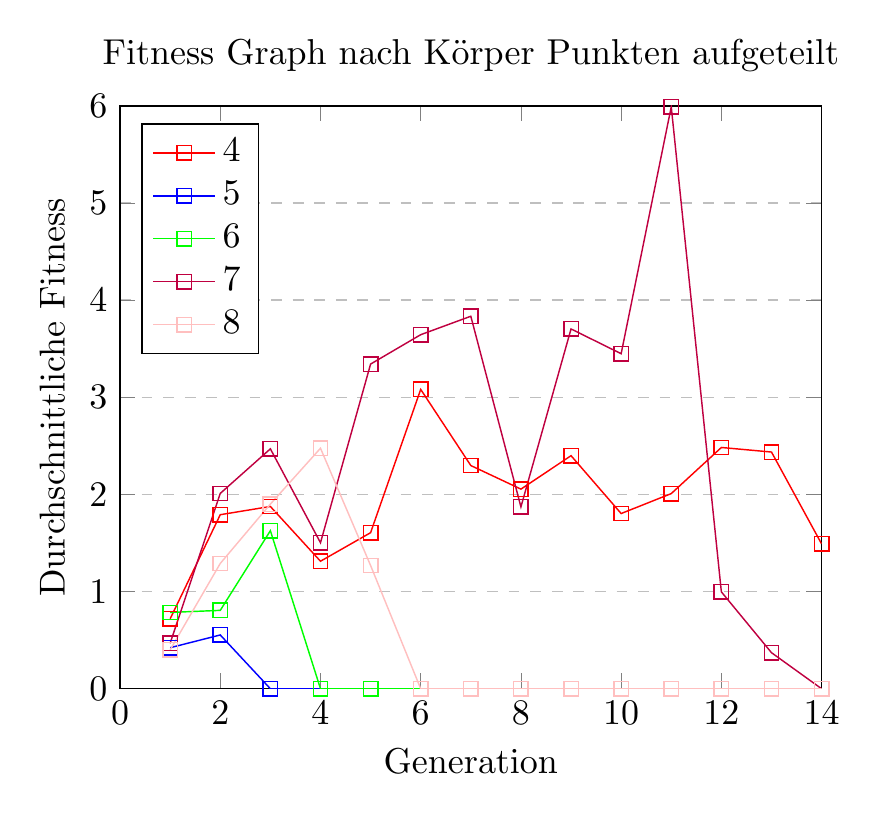
\begin{tikzpicture}[scale=1.3]
\begin{axis}[
    title={Fitness Graph nach Körper Punkten aufgeteilt},
    xlabel={Generation},
    ylabel={Durchschnittliche Fitness},
    xmin=0, xmax=14,
    ymin=0, ymax=6,
    xtick={0,2,4,6,8,10,12,14},
    ytick={0,1,2,3,4,5,6},
    legend pos=north west,
    ymajorgrids=true,
    grid style=dashed,
]

\addplot[
    color=red,
    mark=square,
    ]
    coordinates {
		(1,0.7197311288090767)(2,1.7917008390932372)(3,1.8763654203641982)(4,1.3127839017887504)(5,1.606485315324629)(6,3.081845732380266)(7,2.297797014315923)(8,2.055005581999147)(9,2.3994162926548404)(10,1.8036576432900295)(11,2.009064516425133)(12,2.4837885438165532)(13,2.436803859690654)(14,1.4910241046299537)
    };
    \addlegendentry{4}


\addplot[
    color=blue,
    mark=square,
    ]
    coordinates {
	(1,0.42241279780864716)(2,0.5535280124137276)(3,0)(4,0)(5,0)(6,0)(7,0)(8,0)(9,0)(10,0)(11,0)(12,0)(13,0)(14,0)
    };
    \addlegendentry{5}


\addplot[
    color=green,
    mark=square,
    ]
    coordinates {
	(1,0.7854441017622039)(2,0.8068950995802879)(3,1.6271000623703002)(4,0)(5,0)(6,0)(7,0)(8,0)(9,0)(10,0)(11,0)(12,0)(13,0)(14,0)
    };
    \addlegendentry{6}

\addplot[
    color=purple,
    mark=square,
    ]
    coordinates {
		(1,0.4685424281464469)(2,2.0108517235517502)(3,2.4697639744947937)(4,1.503244884001712)(5,3.3424592366328043)(6,3.644894652227138)(7,3.8348696411420136)(8,1.871792603770028)(9,3.70393052816391)(10,3.4490561534961066)(11,5.99130117893219)(12,0.9973328045823358)(13,0.37121231853961945)(14,0)
	};
    \addlegendentry{7}

\addplot[
    color=pink,
    mark=square,
    ]
    coordinates {
		(1,0.4001652509683654)(2,1.2898510225117206)(3,1.9010943668809803)(4,2.4758530855178833)(5,1.268694241841634)(6,0)(7,0)(8,0)(9,0)(10,0)(11,0)(12,0)(13,0)(14,0)
    };
    \addlegendentry{8}

\end{axis}
\end{tikzpicture}

        \caption{Durchschnittliches Individuum pro Anzahl Körperpunkte, Erster Versuch\label{fig:graphBpFirst}}
      \end{figure}

  \section{Zweiter Versuch, parametrisierbare Steuerung ohne Feedback}

    \subsection{Konfiguration}

      \begin{table}[H]
        % !TEX root = ../main.tex

    \begin{tabular}{ | l | l | }
      \hline
      \multicolumn{2}{|c|}{Simulationsparameter} \\
      \hline
      Populationsgrösse & 120 \\ \hline
      Selektionsstrategie & Turnier-basierte Selektion \\ \hline
      Iterationen & ca. 13900 \\ \hline
      Iterations Dauer & 30s \\ \hline
      Schwierigkeit erhöhen pro & 100 Generationen \\ \hline
      Steigungs Zuwachs & 0.01 \\ \hline
      Maximale Steigung & 1.0 \\ \hline
      Höchste Y-Koordinate Zuwachs  & 0.02 \\ \hline
      Wahscheinlichkeit Mutation pro Attribut & 0.1 \\ \hline
      Ziel & Allgemeine Lösung \\ \hline
    \end{tabular}

        \caption{Simulationsparameter, Zweiter Versuch}
      \end{table}

    \subsection{Auswertung}

      Interessant zu beobachten ist beim zweiten Versuch,
      dass die Fitness der Individuen erst ab der 1400\@. Generation (siehe Abbildung~\vref{fig:graphSecond})
      wieder abzunehmen beginnt.
      Jedoch ist auch hier wieder ein klarer, wenn auch nicht so starker Abwärtstrend zu erkennen.
      Eine weitere Vermutung, neben dem fehlenden Feedback der Engine, warum die Fitness wieder abzunehmen beginnt,
      ist die zu hohe Wahrscheinlichkeit der Mutation.
      In einem nächsten Versuch muss getestet werden,
      ob niedrigere Mutationswahrscheinlichkeiten einen positiven Effekt auf die langfristige Fitness der Individuen haben.
      Ab ca\@. der 2000\@. Generation beginnt die Fitness wieder rapide zu steigen,
      jedoch ist dies durch einen Fehler der Engine zu erklären.
      Die Individuen verhaken sich im Boden und beginnen grosse Distanzen durch Hüpfbewegungen zurückzulegen.
      Dieser Fehler kann bereinigt werden indem die Relaxation erhöht und gleichzeitig der Zeitschritt verringert wird,
      diese Parameter sind in~\vref{sec:Konfiguration} beschrieben.

      \begin{figure}
        % !TEX root = ../main.tex

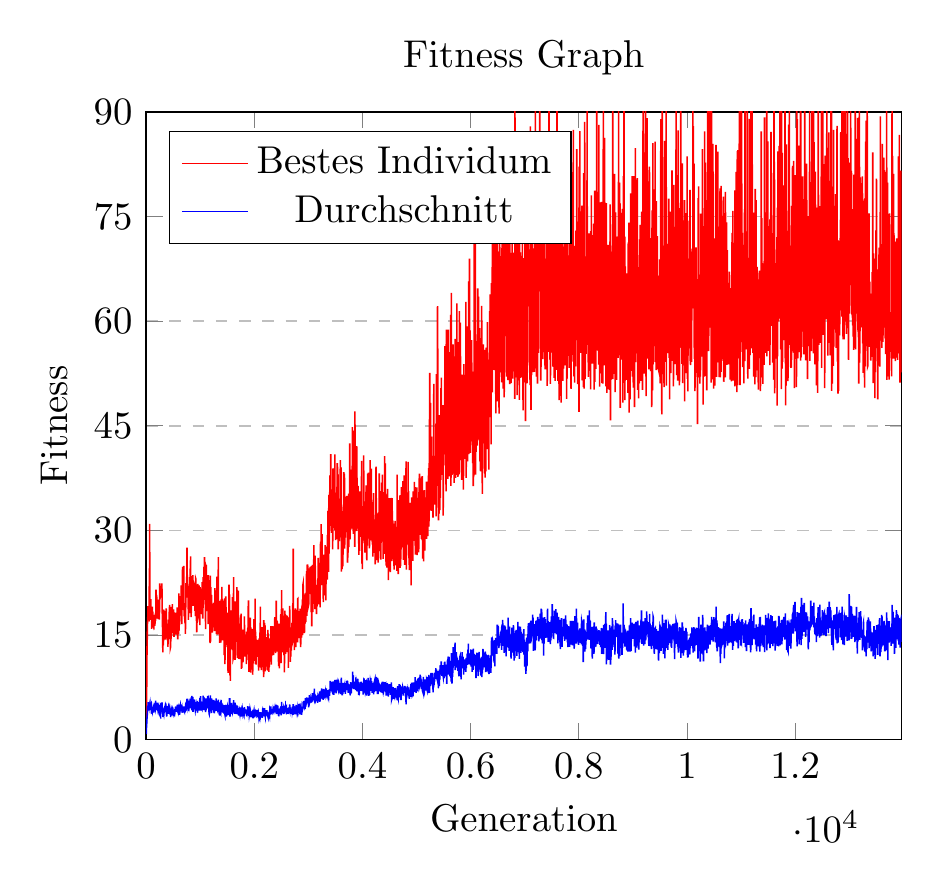
\begin{tikzpicture}[scale=1.4]
\begin{axis}[
    title={Fitness Graph},
    xlabel={Generation},
    ylabel={Fitness},
    xmin=0, xmax=13968,
    ymin=0, ymax=90,
    xtick={0,2000,4000,6000,8000,10000,12000},
    ytick={0,15,30,45,60,75,90},
    legend pos=north west,
    ymajorgrids=true,
    grid style=dashed,
]

\addplot[
    color=red,
    mark=none,
    ]
    coordinates {
		(3, 3.5026691754659018)(6, 2.7299986680348714666666666667)(9, 4.5660749276479085)(12, 7.978335062662760333333333333)(15, 10.441663742065429666666666667)(18, 14.521570841471354666666666667)(21, 14.418912887573242333333333333)(24, 16.171615600585937666666666667)(27, 17.09874153137207)(30, 16.763207753499348666666666667)(33, 19.150664647420247333333333333)(36, 17.231171925862630333333333333)(39, 17.807218551635742)(42, 19.005100250244140333333333333)(45, 18.044162750244140333333333333)(48, 17.422129313151041666666666667)(51, 17.34295082092285)(54, 17.300490697224935333333333333)(57, 21.190504709879557333333333333)(60, 22.481410344441731666666666667)(63, 23.585902531941731666666666667)(66, 30.944686253865559)(69, 19.887764612833657666666666667)(72, 17.175432840983073)(75, 18.339933395385742)(78, 17.370771408081055)(81, 18.195515314737956)(84, 18.219132741292317666666666667)(87, 20.131423950195312)(90, 19.171792348225910666666666667)(93, 17.385962804158528333333333333)(96, 18.548767089843749333333333333)(99, 18.279183705647786666666666667)(102, 15.877882639567057333333333333)(105, 16.173494021097819)(108, 17.154510180155436666666666667)(111, 16.776933670043945666666666667)(114, 17.323849995930989333333333333)(117, 19.067775090535482)(120, 16.185153961181640666666666667)(123, 17.403374354044596333333333333)(126, 18.341417312622070333333333333)(129, 16.881416320800781666666666667)(132, 16.262324333190917666666666667)(135, 16.196570396423340333333333333)(138, 16.669769922892253)(141, 16.378852526346842333333333333)(144, 16.322947820027669333333333333)(147, 17.885283152262370)(150, 17.111034393310547)(153, 17.325805028279622666666666667)(156, 17.405858993530273666666666667)(159, 16.461177825927733666666666667)(162, 16.331277529398600)(165, 17.478046417236328)(168, 16.628599166870117)(171, 18.048837025960286666666666667)(174, 17.074808756510416666666666667)(177, 18.210189183553059666666666667)(180, 17.430742899576823)(183, 21.494721094767252666666666667)(186, 17.656391779581706)(189, 18.903703053792317333333333333)(192, 18.822358449300129666666666667)(195, 20.757602055867513333333333333)(198, 20.154349009195964)(201, 19.359099706013997333333333333)(204, 17.365943908691406666666666667)(207, 19.495356241861979333333333333)(210, 17.779101689656575666666666667)(213, 19.405440012613932)(216, 19.308275858561198333333333333)(219, 18.105644226074218333333333333)(222, 18.201404571533202333333333333)(225, 17.933925628662109)(228, 18.49417495727539)(231, 17.276689529418945333333333333)(234, 20.068886439005533666666666667)(237, 19.497765223185221333333333333)(240, 19.800477345784505666666666667)(243, 19.243587493896484333333333333)(246, 17.214460690816243)(249, 19.519630432128905666666666667)(252, 22.403699874877930)(255, 20.091201782226562666666666667)(258, 20.355915069580078666666666667)(261, 21.097489674886067666666666667)(264, 20.634696324666341666666666667)(267, 22.030264536539713666666666667)(270, 20.551650365193685)(273, 21.688217163085937666666666667)(276, 21.731092453002929666666666667)(279, 21.084321975708007666666666667)(282, 20.365404764811198333333333333)(285, 21.348725636800129666666666667)(288, 20.475877126057942666666666667)(291, 22.384917577107747333333333333)(294, 21.504141489664713666666666667)(297, 19.601343154907226)(300, 17.412584940592448666666666667)(303, 16.355898221333821333333333333)(306, 15.495242118835449)(309, 12.523416201273600333333333333)(312, 15.056746164957682333333333333)(315, 15.749749819437662333333333333)(318, 13.498574574788411666666666667)(321, 17.838491439819335666666666667)(324, 14.118158340454101666666666667)(327, 18.482812563578287666666666667)(330, 18.634614944458007333333333333)(333, 16.443011601765950666666666667)(336, 15.653821627298991)(339, 16.457326571146647333333333333)(342, 14.361908276875813333333333333)(345, 17.230359077453613)(348, 18.406883239746094333333333333)(351, 15.774906794230143)(354, 14.339980125427246)(357, 16.037865320841471333333333333)(360, 16.463355382283528333333333333)(363, 18.211919148763021333333333333)(366, 16.585960070292154666666666667)(369, 15.788853645324707)(372, 18.821111043294270666666666667)(375, 17.657884597778320333333333333)(378, 15.845036188761393666666666667)(381, 15.762518882751465)(384, 15.913424491882324333333333333)(387, 14.527972221374512)(390, 16.234847704569498333333333333)(393, 15.254082679748535333333333333)(396, 15.374973932902018333333333333)(399, 15.842110951741536333333333333)(402, 13.316347757975260333333333333)(405, 13.765630404154459666666666667)(408, 16.144108136494954333333333333)(411, 16.829192479451497666666666667)(414, 17.199415524800618333333333333)(417, 14.901839256286621333333333333)(420, 16.525073369344075333333333333)(423, 17.194257736206055)(426, 14.392021814982096666666666667)(429, 19.020365715026856)(432, 17.360469818115234333333333333)(435, 19.332433064778646)(438, 15.209472338358561333333333333)(441, 16.101668039957682)(444, 15.837563514709472666666666667)(447, 17.328587532043457)(450, 13.193400382995605666666666667)(453, 13.297131856282552333333333333)(456, 15.189655303955078)(459, 14.080198923746745)(462, 15.266765912373860666666666667)(465, 19.048062642415364333333333333)(468, 17.900293350219726666666666667)(471, 14.892037073771159)(474, 15.541549364725748666666666667)(477, 17.768900553385417)(480, 18.347959518432617333333333333)(483, 17.196671485900878666666666667)(486, 19.431061426798503)(489, 16.469435691833496)(492, 15.265762011210123333333333333)(495, 17.068894704182942333333333333)(498, 17.819613774617512666666666667)(501, 15.780100504557291666666666667)(504, 17.329372723897298333333333333)(507, 17.429374059041341666666666667)(510, 18.664663950602213666666666667)(513, 17.258361180623372333333333333)(516, 14.733423550923665333333333333)(519, 15.239904721577961666666666667)(522, 17.396177291870117)(525, 15.291228294372558666666666667)(528, 17.215192794799805)(531, 17.096087455749512333333333333)(534, 16.550295511881510666666666667)(537, 18.080061594645182333333333333)(540, 17.882042566935221333333333333)(543, 17.529334704081217333333333333)(546, 18.202440261840820)(549, 15.056120872497558666666666667)(552, 17.699862480163574333333333333)(555, 16.361063321431477333333333333)(558, 17.786322275797525666666666667)(561, 16.443218866984049666666666667)(564, 15.422432899475097666666666667)(567, 15.591411590576171666666666667)(570, 16.366804122924804)(573, 17.651533444722493666666666667)(576, 18.943721771240234)(579, 17.499020894368489333333333333)(582, 18.752608617146810)(585, 14.381545702616373666666666667)(588, 17.257256507873535333333333333)(591, 15.190687497456868333333333333)(594, 16.428544680277506333333333333)(597, 16.867122968037923333333333333)(600, 15.142551740010579333333333333)(603, 15.707189877827962666666666667)(606, 20.951498349507649666666666667)(609, 15.623902956644694)(612, 19.715829213460286333333333333)(615, 16.720209121704101333333333333)(618, 16.694998423258463333333333333)(621, 17.246784210205078333333333333)(624, 19.352963129679362)(627, 18.885665257771809666666666667)(630, 20.240613301595052)(633, 17.815168698628744)(636, 20.579718907674154)(639, 18.622763951619466)(642, 18.279522577921550)(645, 19.778446197509765666666666667)(648, 22.108401616414388)(651, 20.015003204345702666666666667)(654, 18.077422459920247666666666667)(657, 19.983230590820312666666666667)(660, 16.544006029764811)(663, 19.638740539550780666666666667)(666, 19.863269805908202666666666667)(669, 19.917678197224935)(672, 24.015675226847331)(675, 24.756165186564127)(678, 19.629221598307291666666666667)(681, 19.786239624023437666666666667)(684, 18.604268391927083666666666667)(687, 20.509515762329102)(690, 19.122410456339518333333333333)(693, 20.833812077840169)(696, 24.911704381306965666666666667)(699, 20.965639750162760)(702, 17.755994160970052666666666667)(705, 18.625707626342772666666666667)(708, 19.469023704528809)(711, 17.233029047648112333333333333)(714, 18.355920791625976333333333333)(717, 18.006869633992513333333333333)(720, 16.634446144104004)(723, 18.661292394002278666666666667)(726, 15.168078422546386333333333333)(729, 16.172105789184570666666666667)(732, 18.909543991088867)(735, 19.143335342407226666666666667)(738, 22.439132054646809333333333333)(741, 21.272963205973307)(744, 22.044682184855143666666666667)(747, 20.760318756103515333333333333)(750, 23.385674794514974)(753, 21.112805684407552333333333333)(756, 27.535722096761066666666666667)(759, 20.367950439453124666666666667)(762, 23.659899393717448333333333333)(765, 22.355230967203776666666666667)(768, 20.981094996134440333333333333)(771, 22.02741559346517)(774, 21.412460327148437666666666667)(777, 19.903480529785156666666666667)(780, 18.649070739746093666666666667)(783, 17.162910779317220)(786, 19.680724461873372333333333333)(789, 19.746308644612630666666666667)(792, 20.881357828776042)(795, 21.593050003051757666666666667)(798, 20.985826492309570333333333333)(801, 20.077803293863932666666666667)(804, 21.378049850463867)(807, 23.290973027547200)(810, 21.155371348063150666666666667)(813, 18.134809176127115666666666667)(816, 24.533751169840494666666666667)(819, 23.252031326293945)(822, 26.277108510335286666666666667)(825, 22.267113367716472)(828, 20.826401074727376666666666667)(831, 22.905265808105469)(834, 17.570677121480306)(837, 22.736286799112955333333333333)(840, 23.426371892293295)(843, 20.926616668701171666666666667)(846, 21.447165171305338666666666667)(849, 22.026155471801757666666666667)(852, 19.436107635498046666666666667)(855, 20.190958023071289333333333333)(858, 20.876148859659830333333333333)(861, 21.748655319213866666666666667)(864, 23.586064020792643333333333333)(867, 19.163736661275228)(870, 21.059516906738281666666666667)(873, 22.010829925537109333333333333)(876, 20.519723892211914)(879, 22.472056706746419)(882, 22.385902404785156666666666667)(885, 22.091407140096028333333333333)(888, 21.076145172119140333333333333)(891, 20.253739039103190)(894, 22.108599980672200333333333333)(897, 21.180962880452473666666666667)(900, 20.684691111246744)(903, 18.468689600626628333333333333)(906, 21.415523529052734666666666667)(909, 19.437213897705078666666666667)(912, 17.694228490193685333333333333)(915, 19.898667017618816)(918, 23.081312179565430)(921, 23.008818944295247)(924, 21.067783355712890)(927, 19.558177947998047333333333333)(930, 17.014592806498210)(933, 19.768293698628743333333333333)(936, 15.386802355448404666666666667)(939, 18.459824879964192666666666667)(942, 18.651337941487630333333333333)(945, 20.494495391845703333333333333)(948, 20.673313776652018333333333333)(951, 16.978613535563151)(954, 17.043224970499675)(957, 22.327934265136719)(960, 20.560717264811197666666666667)(963, 19.542051315307617666666666667)(966, 17.384638786315918)(969, 20.466252644856770666666666667)(972, 20.548820495605468666666666667)(975, 17.893052260080973333333333333)(978, 20.678561528523763)(981, 22.129224141438802)(984, 18.451963106791178666666666667)(987, 18.435146331787108666666666667)(990, 20.602569580078124666666666667)(993, 16.418079694112141666666666667)(996, 21.132942199707031)(999, 21.848304112752279)(1002, 20.794635136922200333333333333)(1005, 18.665018081665039)(1008, 19.980035463968912666666666667)(1011, 21.064252217610676666666666667)(1014, 20.802453994750976)(1017, 20.486010551452636666666666667)(1020, 19.780045827229817666666666667)(1023, 21.658372243245443333333333333)(1026, 18.601906140645345333333333333)(1029, 18.029498736063639)(1032, 19.514555295308430666666666667)(1035, 22.575272242228189666666666667)(1038, 21.452608744303385)(1041, 18.547676722208659)(1044, 18.618663152058919333333333333)(1047, 17.363703727722168)(1050, 22.601516087849935)(1053, 18.904766082763672)(1056, 23.295391082763672)(1059, 20.069313685099283666666666667)(1062, 20.224894205729166666666666667)(1065, 22.117900212605794)(1068, 24.778525670369466666666666667)(1071, 24.582853953043620333333333333)(1074, 22.654015223185220666666666667)(1077, 21.992819468180338333333333333)(1080, 26.179356257120768)(1083, 20.721071879069010666666666667)(1086, 23.127464930216471666666666667)(1089, 23.737427393595377)(1092, 23.985807418823241)(1095, 17.471837361653645666666666667)(1098, 17.291367848714192666666666667)(1101, 15.841295560201009333333333333)(1104, 22.499256134033202666666666667)(1107, 24.873631795247395333333333333)(1110, 24.789241790771484333333333333)(1113, 24.810760498046875)(1116, 18.414948145548502333333333333)(1119, 20.254004796346028666666666667)(1122, 23.451162338256836)(1125, 22.063253402709961)(1128, 19.886782010396321333333333333)(1131, 20.927921295166015)(1134, 22.657589594523112333333333333)(1137, 20.754069328308105)(1140, 20.956331253051758)(1143, 21.989709854125976333333333333)(1146, 16.544336001078287666666666667)(1149, 23.573561986287435333333333333)(1152, 23.102644602457681666666666667)(1155, 21.934780756632486333333333333)(1158, 18.805592854817708333333333333)(1161, 21.473442077636718666666666667)(1164, 19.327794392903646333333333333)(1167, 17.734912236531575666666666667)(1170, 21.600056330362955666666666667)(1173, 19.536657333374023333333333333)(1176, 22.859944025675455333333333333)(1179, 20.611092885335286666666666667)(1182, 13.832094192504883)(1185, 20.419626235961913333333333333)(1188, 23.511899948120116666666666667)(1191, 14.037493069966634)(1194, 20.826451301574707)(1197, 21.870351473490397666666666667)(1200, 17.452650070190429333333333333)(1203, 18.849794387817383)(1206, 18.989405949910481666666666667)(1209, 19.402509689331054333333333333)(1212, 20.746188799540202)(1215, 17.430843989054362)(1218, 17.388534863789876333333333333)(1221, 15.849085807800293)(1224, 15.344234148661295333333333333)(1227, 16.672961552937825333333333333)(1230, 17.540195147196451666666666667)(1233, 16.993474960327148333333333333)(1236, 18.845077196756998333333333333)(1239, 16.098104794820149666666666667)(1242, 19.458169619242350333333333333)(1245, 19.293249289194743)(1248, 17.673692385355631666666666667)(1251, 19.601758956909180)(1254, 17.324533780415852666666666667)(1257, 18.906299591064453)(1260, 18.781658172607422)(1263, 15.541289965311686333333333333)(1266, 18.676082928975423666666666667)(1269, 18.558267593383789)(1272, 21.716709454854329333333333333)(1275, 18.031782150268554333333333333)(1278, 21.410033543904622666666666667)(1281, 20.496489206949870333333333333)(1284, 20.791833877563476333333333333)(1287, 15.613190015157063666666666667)(1290, 15.801359494527181)(1293, 16.452321052551269666666666667)(1296, 20.855647404988606666666666667)(1299, 15.108781814575194666666666667)(1302, 19.115404764811199)(1305, 18.645910263061523666666666667)(1308, 23.363480250040689666666666667)(1311, 17.425821145375569333333333333)(1314, 18.178822199503580666666666667)(1317, 17.455352147420246666666666667)(1320, 15.057139555613200333333333333)(1323, 20.063439051310221)(1326, 17.969309488932292)(1329, 18.928105036417643333333333333)(1332, 16.416444142659504666666666667)(1335, 26.156447728474935)(1338, 19.436379114786783333333333333)(1341, 18.237249692281087666666666667)(1344, 17.814247767130533333333333333)(1347, 15.149911244710286333333333333)(1350, 16.464077313741048)(1353, 19.678281784057617666666666667)(1356, 19.882793426513672)(1359, 13.878007253011067333333333333)(1362, 19.186687469482422)(1365, 18.303167978922526)(1368, 18.815467198689779)(1371, 14.412695884704590)(1374, 16.420605977376302)(1377, 16.669878959655761666666666667)(1380, 13.911554018656412666666666667)(1383, 18.32962163289388)(1386, 20.112232844034830666666666667)(1389, 17.450121561686198)(1392, 19.530625661214193)(1395, 18.993592580159505666666666667)(1398, 16.836820284525553333333333333)(1401, 21.913599014282226666666666667)(1404, 19.134263356526692666666666667)(1407, 18.200028101603190)(1410, 20.159044901529948333333333333)(1413, 17.373611768086751)(1416, 14.223886171976725)(1419, 14.613575935363769333333333333)(1422, 16.763226826985677333333333333)(1425, 15.369965553283691333333333333)(1428, 18.036986351013183666666666667)(1431, 19.933842976888020666666666667)(1434, 15.464130719502767)(1437, 15.456353187561035666666666667)(1440, 19.519001007080079333333333333)(1443, 12.097126642862955666666666667)(1446, 19.493436177571614666666666667)(1449, 19.147184689839681333333333333)(1452, 20.262948354085286333333333333)(1455, 18.787954012552897)(1458, 10.813223203023274666666666667)(1461, 16.396568616231282666666666667)(1464, 13.589297294616699333333333333)(1467, 15.179315249125163)(1470, 15.173065185546875)(1473, 20.523902893066406666666666667)(1476, 19.225618680318197)(1479, 18.408558527628581333333333333)(1482, 17.818369547526042333333333333)(1485, 16.929470062255859)(1488, 16.050029436747233333333333333)(1491, 17.449936866760254)(1494, 15.214241663614908666666666667)(1497, 17.572386423746744666666666667)(1500, 13.258760293324788666666666667)(1503, 17.188062032063802)(1506, 18.222972234090169333333333333)(1509, 16.057131449381510666666666667)(1512, 12.811008771260579333333333333)(1515, 9.583032131195068333333333333)(1518, 14.557819048563639333333333333)(1521, 15.245162645975748666666666667)(1524, 16.670456568400065)(1527, 16.314295450846354)(1530, 16.965147654215495)(1533, 22.236002604166666666666666667)(1536, 13.764509518941243333333333333)(1539, 17.520102818806966333333333333)(1542, 20.832972844441731333333333333)(1545, 16.603044827779134333333333333)(1548, 16.416458447774251666666666667)(1551, 9.2035603523254395)(1554, 14.634753863016764666666666667)(1557, 8.416567007700602)(1560, 12.902805010477701666666666667)(1563, 16.058704694112142)(1566, 15.063086191813151333333333333)(1569, 18.541164398193359333333333333)(1572, 17.305889447530110666666666667)(1575, 18.153268814086914)(1578, 16.385224024454752666666666667)(1581, 18.438009262084961)(1584, 13.549075444539388333333333333)(1587, 14.822508494059244666666666667)(1590, 17.312866210937500333333333333)(1593, 13.015309333801269666666666667)(1596, 20.419997533162435)(1599, 18.138094584147135333333333333)(1602, 12.814065615336100333333333333)(1605, 14.334507306416829333333333333)(1608, 14.906174659729004)(1611, 11.691999435424804666666666667)(1614, 11.800309499104817666666666667)(1617, 23.284102121988932)(1620, 16.927782058715820333333333333)(1623, 11.670757293701172)(1626, 17.112202008565266666666666667)(1629, 17.168022155761719)(1632, 13.302044550577799666666666667)(1635, 14.602522532145182)(1638, 13.275313536326090166666666667)(1641, 16.885943412780762)(1644, 11.424850304921468)(1647, 19.811330159505208666666666667)(1650, 18.613599141438802333333333333)(1653, 17.896269480387370333333333333)(1656, 14.878837267557779666666666667)(1659, 14.363168716430664)(1662, 18.979516029357910333333333333)(1665, 15.106775601704915666666666667)(1668, 15.399099985758464)(1671, 14.015114466349284)(1674, 18.113166173299154333333333333)(1677, 16.209055900573730333333333333)(1680, 21.854827245076497333333333333)(1683, 15.846724669138590333333333333)(1686, 11.692322731018066666666666667)(1689, 14.767835299173990666666666667)(1692, 16.242625872294108)(1695, 14.608222643534342666666666667)(1698, 15.720141092936197666666666667)(1701, 12.272763888041178666666666667)(1704, 21.361811637878419)(1707, 13.871091206868489333333333333)(1710, 12.052514394124349)(1713, 13.268227577209472666666666667)(1716, 11.590331713358561)(1719, 16.618461290995280)(1722, 15.192735989888508666666666667)(1725, 14.355896949768067)(1728, 11.528342247009277333333333333)(1731, 13.863183657328287666666666667)(1734, 14.741689364115397)(1737, 12.272274017333984333333333333)(1740, 14.171046892801920666666666667)(1743, 13.079264322916666333333333333)(1746, 17.796214103698730)(1749, 13.799068768819173333333333333)(1752, 13.962909062703450666666666667)(1755, 17.591655413309733)(1758, 18.068479537963867)(1761, 10.145739237467448)(1764, 13.724089304606119666666666667)(1767, 12.195777098337809)(1770, 10.268823464711507166666666667)(1773, 13.478000958760579333333333333)(1776, 12.798928578694661666666666667)(1779, 12.908177375793457333333333333)(1782, 15.755236943562825666666666667)(1785, 11.514490127563476666666666667)(1788, 15.031810442606608333333333333)(1791, 11.073666731516520166666666667)(1794, 14.072685559590657666666666667)(1797, 12.526501814524332666666666667)(1800, 14.943642934163412)(1803, 12.578530311584472666666666667)(1806, 13.940491676330566)(1809, 13.958862304687499833333333333)(1812, 15.357685089111328333333333333)(1815, 14.812290191650390333333333333)(1818, 17.685353279113768666666666667)(1821, 13.362074851989746)(1824, 14.173908551534016666666666667)(1827, 11.891059875488281333333333333)(1830, 12.152180989583333333333333333)(1833, 13.979230562845866)(1836, 13.409392992655436333333333333)(1839, 15.062341372172037666666666667)(1842, 14.336870034535727)(1845, 13.262096087137858333333333333)(1848, 14.980359077453613333333333333)(1851, 14.715188344319661333333333333)(1854, 10.829480171203613333333333333)(1857, 13.117422739664713333333333333)(1860, 15.472785631815592333333333333)(1863, 12.756698449452718)(1866, 14.8236363728841145)(1869, 14.153721332550048666666666667)(1872, 13.386281649271647)(1875, 13.580901145935058666666666667)(1878, 15.708839416503906)(1881, 16.066858291625976666666666667)(1884, 14.009558995564778666666666667)(1887, 19.129807154337565)(1890, 11.412749608357747333333333333)(1893, 19.973669052124023333333333333)(1896, 11.729620456695556666666666667)(1899, 16.226205190022786333333333333)(1902, 9.700672467549642)(1905, 16.428389231363932)(1908, 14.931810379028320333333333333)(1911, 13.799002329508463333333333333)(1914, 13.569806416829427)(1917, 12.731157302856445666666666667)(1920, 14.704075813293457)(1923, 14.307443141937256)(1926, 17.491844495137532666666666667)(1929, 14.548382123311360666666666667)(1932, 9.602460543314616)(1935, 12.405634721120198666666666667)(1938, 16.091151555379231333333333333)(1941, 14.637384732564290333333333333)(1944, 14.697251637776692666666666667)(1947, 11.417852719624837333333333333)(1950, 12.482875029246012333333333333)(1953, 10.049036979675292666666666667)(1956, 14.579992294311523666666666667)(1959, 13.523715655008952)(1962, 14.037625312805175666666666667)(1965, 15.378574689229329666666666667)(1968, 15.861714998881022)(1971, 9.300172011057535666666666667)(1974, 13.175371170043945333333333333)(1977, 10.949630896250407)(1980, 12.062227249145507666666666667)(1983, 12.779838879903157666666666667)(1986, 13.787154833475748333333333333)(1989, 14.874953905741373666666666667)(1992, 15.688818931579590)(1995, 17.265892346700032333333333333)(1998, 11.275547663370768)(2001, 12.940289815266927)(2004, 11.755432764689127666666666667)(2007, 12.437302589416504)(2010, 13.488001823425293)(2013, 11.718482335408528666666666667)(2016, 20.217704772949218666666666667)(2019, 10.809062163035074666666666667)(2022, 15.694760322570801)(2025, 12.383646170298258666666666667)(2028, 11.759857177734375333333333333)(2031, 14.829676946004231666666666667)(2034, 10.734501520792643)(2037, 14.329010327657063666666666667)(2040, 12.258961041768392)(2043, 12.848457018534342333333333333)(2046, 13.021024703979492)(2049, 12.271020571390787666666666667)(2052, 13.965315818786621)(2055, 11.856611251831054666666666667)(2058, 13.318525632222493333333333333)(2061, 13.770347913106283333333333333)(2064, 13.700511296590169333333333333)(2067, 11.863492965698242)(2070, 13.851579030354817666666666667)(2073, 13.509032249450684)(2076, 14.314915657043457)(2079, 9.8760172526041665)(2082, 11.212491035461426)(2085, 12.256660779317220)(2088, 12.978298187255859666666666667)(2091, 14.516551653544108)(2094, 10.688828150431315)(2097, 11.920814196268717333333333333)(2100, 10.375291506449381333333333333)(2103, 14.528827667236327666666666667)(2106, 15.341035525004068666666666667)(2109, 12.386626561482747333333333333)(2112, 19.067275047302246333333333333)(2115, 12.399932861328125)(2118, 11.970339775085449)(2121, 12.198038101196289)(2124, 11.028739770253499333333333333)(2127, 11.525716940561930333333333333)(2130, 9.951032161712646333333333333)(2133, 13.664949417114257666666666667)(2136, 15.953852653503418333333333333)(2139, 16.135470708211263)(2142, 10.388566652933756333333333333)(2145, 14.080702463785807)(2148, 14.487655003865559666666666667)(2151, 12.278673489888509)(2154, 10.963658650716146)(2157, 14.513177235921223666666666667)(2160, 12.187648455301920666666666667)(2163, 14.077215194702148333333333333)(2166, 12.092718124389648333333333333)(2169, 11.415658315022786666666666667)(2172, 8.949688752492269333333333333)(2175, 17.117136001586914)(2178, 9.404682318369547)(2181, 14.764019012451171666666666667)(2184, 13.512968699137369666666666667)(2187, 12.511734485626220666666666667)(2190, 16.731567382812500)(2193, 11.870844205220540666666666667)(2196, 10.172990163167317833333333333)(2199, 16.379989306131998666666666667)(2202, 9.793940067291259833333333333)(2205, 11.021869341532389333333333333)(2208, 10.790401776631672666666666667)(2211, 13.483893076578775666666666667)(2214, 11.114266872406006)(2217, 14.743169466654459666666666667)(2220, 12.925072352091471333333333333)(2223, 14.049345016479492)(2226, 11.532965660095215)(2229, 11.188976605733235666666666667)(2232, 14.365839322408040333333333333)(2235, 10.909480094909667666666666667)(2238, 12.103100776672363666666666667)(2241, 10.045297463734944666666666667)(2244, 12.273717244466145666666666667)(2247, 9.899119536081950)(2250, 11.949324925740560)(2253, 15.746864954630533666666666667)(2256, 10.980447451273600)(2259, 10.719355106353759666666666667)(2262, 12.580333073933919)(2265, 12.513975461324056)(2268, 10.164386749267578)(2271, 9.704068183898925666666666667)(2274, 12.178644180297851333333333333)(2277, 10.439845720926920666666666667)(2280, 10.836938540140788)(2283, 11.813383420308431)(2286, 13.328648249308268333333333333)(2289, 14.511722564697265333333333333)(2292, 12.515234152475993)(2295, 12.409602801005045333333333333)(2298, 12.960376103719075666666666667)(2301, 14.819076855977376333333333333)(2304, 13.912620703379313333333333333)(2307, 16.284331957499186666666666667)(2310, 11.652295112609863)(2313, 14.796565373738606666666666667)(2316, 10.765446980794271)(2319, 15.646708488464355333333333333)(2322, 15.140541712443034)(2325, 12.032183647155761666666666667)(2328, 14.095926284790039)(2331, 15.314565976460774666666666667)(2334, 16.170185407002767333333333333)(2337, 14.340167363484700666666666667)(2340, 16.274421374003092333333333333)(2343, 15.218097686767578)(2346, 16.212324778238932333333333333)(2349, 12.508281389872233)(2352, 15.071435928344727)(2355, 12.101153055826822666666666667)(2358, 14.047169049580892333333333333)(2361, 16.229875882466634333333333333)(2364, 15.613091468811034666666666667)(2367, 15.193394978841146)(2370, 13.377209027608235333333333333)(2373, 14.165607134501139333333333333)(2376, 17.380193710327148333333333333)(2379, 12.633754571278890333333333333)(2382, 17.576814969380696666666666667)(2385, 16.575451215108235666666666667)(2388, 15.265597979227702333333333333)(2391, 16.279538790384928333333333333)(2394, 12.387263615926107)(2397, 17.20463498433431)(2400, 14.107165336608886666666666667)(2403, 17.268020311991374)(2406, 19.918040593465169333333333333)(2409, 13.309980392456054666666666667)(2412, 13.153381029764811333333333333)(2415, 12.633044242858886666666666667)(2418, 13.948627471923828)(2421, 13.199584960937499666666666667)(2424, 17.066623369852702)(2427, 15.908936500549316666666666667)(2430, 13.264404932657877666666666667)(2433, 13.897481600443521666666666667)(2436, 15.451669057210286333333333333)(2439, 15.381483078002929666666666667)(2442, 14.701338768005371)(2445, 11.173736254374186)(2448, 13.159769376118978)(2451, 10.519706726074218666666666667)(2454, 12.824191093444824333333333333)(2457, 12.950230916341146)(2460, 16.615091323852539)(2463, 10.217344125111898)(2466, 15.333572387695312666666666667)(2469, 14.346261024475097666666666667)(2472, 14.062861760457356333333333333)(2475, 15.244593620300293)(2478, 11.541880925496419333333333333)(2481, 12.407963752746582333333333333)(2484, 14.635947227478027333333333333)(2487, 13.458057244618733666666666667)(2490, 17.997376759847005666666666667)(2493, 17.500674565633138)(2496, 10.972720464070638)(2499, 17.030896186828613333333333333)(2502, 14.447776158650716333333333333)(2505, 21.448421478271484)(2508, 17.197102228800455666666666667)(2511, 12.808719635009766)(2514, 12.502570788065592333333333333)(2517, 17.788989384969076)(2520, 13.936044057210286333333333333)(2523, 16.091764132181803333333333333)(2526, 17.592680931091308666666666667)(2529, 18.811428070068359333333333333)(2532, 14.502310434977213666666666667)(2535, 16.501662890116374)(2538, 15.250459353129069)(2541, 14.285635630289713666666666667)(2544, 13.081665674845377666666666667)(2547, 12.131482760111490666666666667)(2550, 14.774655977884928333333333333)(2553, 17.793275515238444)(2556, 9.628184318542480333333333333)(2559, 11.278748035430907666666666667)(2562, 16.081038157145182333333333333)(2565, 18.509153366088867333333333333)(2568, 16.600356101989746333333333333)(2571, 16.921151796976725666666666667)(2574, 17.026169776916504)(2577, 12.310787836710612)(2580, 14.307010968526204333333333333)(2583, 16.881591796875000)(2586, 17.842793782552083333333333333)(2589, 15.692459742228189666666666667)(2592, 14.820601145426432666666666667)(2595, 15.850878397623697666666666667)(2598, 13.747943242390951)(2601, 13.287535031636556)(2604, 12.553990364074707)(2607, 17.780934969584148)(2610, 15.377448081970215)(2613, 17.606544494628906)(2616, 14.407866477966308666666666667)(2619, 17.536638577779134)(2622, 16.030163764953614)(2625, 14.127531687418619666666666667)(2628, 14.555210113525391)(2631, 10.301555633544921666666666667)(2634, 16.850344657897948333333333333)(2637, 15.980058352152506)(2640, 13.423752148946126)(2643, 16.115664800008138)(2646, 14.514729181925455666666666667)(2649, 14.117145220438639666666666667)(2652, 14.608684539794921666666666667)(2655, 19.163408279418945333333333333)(2658, 15.444967269897461333333333333)(2661, 15.415463765462239)(2664, 15.478538831075032666666666667)(2667, 11.162200291951497666666666667)(2670, 15.268878936767578)(2673, 11.875884056091308333333333333)(2676, 12.139689445495605666666666667)(2679, 14.410006523132324666666666667)(2682, 14.787509282430013)(2685, 12.762715657552083333333333333)(2688, 13.291512171427409)(2691, 15.253931681315104333333333333)(2694, 15.065024693806966333333333333)(2697, 16.712062835693359666666666667)(2700, 13.507224400838216333333333333)(2703, 16.897562344868977666666666667)(2706, 13.795772552490234333333333333)(2709, 15.023272196451823333333333333)(2712, 19.571878751118977666666666667)(2715, 14.234549840291341333333333333)(2718, 14.800317764282226333333333333)(2721, 27.380140940348307)(2724, 18.591458320617675666666666667)(2727, 15.174568176269531333333333333)(2730, 15.923233032226562)(2733, 17.428669929504394666666666667)(2736, 15.425019900004069)(2739, 15.813334465026855666666666667)(2742, 12.821993192036946666666666667)(2745, 15.941940943400065)(2748, 13.687249501546223666666666667)(2751, 13.407430648803711)(2754, 18.601691881815592333333333333)(2757, 15.286458333333333333333333333)(2760, 18.827753702799478666666666667)(2763, 13.719309806823730666666666667)(2766, 17.222893079121907333333333333)(2769, 13.264238039652506666666666667)(2772, 17.879815737406413)(2775, 18.605416297912597666666666667)(2778, 18.209503173828125)(2781, 16.183795928955078)(2784, 17.162189801534017)(2787, 17.737683931986490666666666667)(2790, 18.050531387329102)(2793, 14.879343986511230666666666667)(2796, 18.624065717061360333333333333)(2799, 13.949456532796224)(2802, 20.180907249450683333333333333)(2805, 20.207312901814778666666666667)(2808, 17.334253629048665333333333333)(2811, 17.186771710713704333333333333)(2814, 16.166442235310872666666666667)(2817, 16.789176623026529666666666667)(2820, 15.031668027242024666666666667)(2823, 16.074461301167806)(2826, 15.987538337707519333333333333)(2829, 16.896652221679688)(2832, 15.247125307718912666666666667)(2835, 14.571395238240560)(2838, 18.415350278218586666666666667)(2841, 16.087775866190592333333333333)(2844, 15.481044769287109666666666667)(2847, 15.997900009155273333333333333)(2850, 18.764441808064779333333333333)(2853, 15.178045272827148333333333333)(2856, 13.256812731424967)(2859, 14.935926437377929666666666667)(2862, 13.652737935384114333333333333)(2865, 17.061707178751627333333333333)(2868, 14.697249412536621)(2871, 15.192789395650227666666666667)(2874, 14.643582979838053666666666667)(2877, 15.013942400614420666666666667)(2880, 17.299413363138834666666666667)(2883, 19.216973622639974)(2886, 18.548596382141113333333333333)(2889, 20.113208770751953)(2892, 14.979093551635742)(2895, 17.762126286824544)(2898, 16.597009976704915333333333333)(2901, 22.278225580851236666666666667)(2904, 22.404014587402343666666666667)(2907, 21.518776575724284)(2910, 17.950075785319010666666666667)(2913, 19.992960611979167)(2916, 18.851096471150715666666666667)(2919, 18.019896189371744333333333333)(2922, 18.400312741597494)(2925, 19.377209981282551666666666667)(2928, 15.252424875895182)(2931, 19.194860776265462666666666667)(2934, 18.273726463317871333333333333)(2937, 20.788637797037760333333333333)(2940, 16.633715947469075333333333333)(2943, 17.581739743550618666666666667)(2946, 20.957426071166992333333333333)(2949, 18.913047790527343666666666667)(2952, 16.863976160685222)(2955, 19.549786567687988333333333333)(2958, 20.651709238688150666666666667)(2961, 20.787580490112304666666666667)(2964, 22.969286600748697666666666667)(2967, 24.161702473958333333333333333)(2970, 20.605837504069011)(2973, 17.740303675333659333333333333)(2976, 25.094192504882812666666666667)(2979, 22.173689524332682666666666667)(2982, 20.595956166585286666666666667)(2985, 20.713253021240235)(2988, 25.115977605183919333333333333)(2991, 22.400958379109701)(2994, 22.816919962565104666666666667)(2997, 22.674887339274088)(3000, 22.392472585042318)(3003, 19.242459615071614)(3006, 19.345945994059245)(3009, 19.563964843749999333333333333)(3012, 21.298390706380208333333333333)(3015, 24.562220255533854)(3018, 22.803634007771810666666666667)(3021, 23.789862314860025333333333333)(3024, 22.992289861043294666666666667)(3027, 21.391913096110025666666666667)(3030, 22.755247116088867333333333333)(3033, 24.762284596761066666666666667)(3036, 22.194883346557617666666666667)(3039, 22.558258374532064)(3042, 22.420287450154623333333333333)(3045, 20.844621022542317666666666667)(3048, 23.042364756266276)(3051, 18.274934768676757333333333333)(3054, 24.876995722452799333333333333)(3057, 23.872711817423502)(3060, 23.712461471557617)(3063, 16.245976448059082)(3066, 22.114028612772623666666666667)(3069, 24.282489776611328)(3072, 24.054532368977865333333333333)(3075, 25.040309270222981666666666667)(3078, 19.038053512573242333333333333)(3081, 18.267131805419922333333333333)(3084, 19.438337961832682333333333333)(3087, 19.511944452921549)(3090, 20.544617970784504666666666667)(3093, 19.974342346191406666666666667)(3096, 24.301672617594400666666666667)(3099, 24.708489735921225)(3102, 27.881371180216471)(3105, 21.461116154988607)(3108, 20.722254435221354)(3111, 21.657981872558594333333333333)(3114, 23.514129638671874333333333333)(3117, 24.673858642578125)(3120, 23.426760991414388)(3123, 18.695625623067220)(3126, 26.376476287841797)(3129, 21.534475962320963333333333333)(3132, 19.680524190266927)(3135, 19.472858428955078333333333333)(3138, 21.377410252888996666666666667)(3141, 21.551267941792806)(3144, 22.188949584960938)(3147, 21.339326222737630333333333333)(3150, 17.985674540201822666666666667)(3153, 20.981700261433918666666666667)(3156, 20.217420578002929666666666667)(3159, 20.923086166381836)(3162, 19.115626017252604)(3165, 20.403514862060546666666666667)(3168, 21.368155797322591333333333333)(3171, 22.914804458618163333333333333)(3174, 20.976097742716471)(3177, 19.538029988606771333333333333)(3180, 26.067595799763997333333333333)(3183, 21.675702412923176666666666667)(3186, 23.229841232299803333333333333)(3189, 19.405776341756185)(3192, 21.622027079264323333333333333)(3195, 21.904973983764648)(3198, 25.355178833007812333333333333)(3201, 20.984569549560547333333333333)(3204, 24.435869216918945666666666667)(3207, 23.276311874389649333333333333)(3210, 21.214483261108398)(3213, 23.037848790486653333333333333)(3216, 18.968468983968098666666666667)(3219, 26.094275156656901)(3222, 21.465155283610026)(3225, 28.382350921630860)(3228, 25.959434509277343333333333333)(3231, 23.381027221679687333333333333)(3234, 27.733896891276041666666666667)(3237, 30.886645634969076333333333333)(3240, 23.518974939982096333333333333)(3243, 27.770004908243814666666666667)(3246, 28.551944096883138)(3249, 22.160178502400716)(3252, 29.470299402872720666666666667)(3255, 24.028015136718750333333333333)(3258, 24.676852544148762666666666667)(3261, 24.957261403401693)(3264, 23.419759114583334333333333333)(3267, 24.715241114298502)(3270, 23.743499755859374666666666667)(3273, 25.013111114501953333333333333)(3276, 19.707225799560547)(3279, 23.633520762125651)(3282, 26.041237513224283333333333333)(3285, 22.177407582600911666666666667)(3288, 26.509841283162434666666666667)(3291, 21.661979039510091)(3294, 20.848302205403646333333333333)(3297, 22.164637883504231666666666667)(3300, 25.597141265869140666666666667)(3303, 23.617099761962890)(3306, 22.429885864257812666666666667)(3309, 27.890953063964843)(3312, 20.675995508829752333333333333)(3315, 22.641960144042968)(3318, 24.150896072387695666666666667)(3321, 24.03614616394043)(3324, 19.963478724161784333333333333)(3327, 24.239498774210612333333333333)(3330, 23.088647842407226666666666667)(3333, 25.843766530354818333333333333)(3336, 25.428576787312824666666666667)(3339, 24.324990590413411333333333333)(3342, 25.787879943847656)(3345, 27.684725443522135333333333333)(3348, 24.137653350830078333333333333)(3351, 22.944098790486653666666666667)(3354, 29.365108489990234333333333333)(3357, 24.113070805867512333333333333)(3360, 26.393323262532553333333333333)(3363, 32.815168380737304666666666667)(3366, 26.97671381632487)(3369, 25.880526860555013)(3372, 24.049125671386718666666666667)(3375, 25.925037384033203)(3378, 35.10398292541504)(3381, 27.283329010009766)(3384, 26.662520090738932333333333333)(3387, 28.329247792561849)(3390, 32.895220438639322666666666667)(3393, 32.529525121053058666666666667)(3396, 35.659529368082682)(3399, 37.903059641520183)(3402, 31.11586316426595)(3405, 32.217233657836913666666666667)(3408, 32.344102223714193333333333333)(3411, 31.107992172241211)(3414, 40.942501703898111)(3417, 30.721604029337565333333333333)(3420, 31.276477813720702666666666667)(3423, 30.688535690307616333333333333)(3426, 30.653217951456706)(3429, 29.661028544108073)(3432, 35.876996994018555333333333333)(3435, 32.764472961425781666666666667)(3438, 33.676670074462891)(3441, 30.942835489908855333333333333)(3444, 32.73678970336914)(3447, 30.534257253011067666666666667)(3450, 27.287888844807943)(3453, 35.758522033691405333333333333)(3456, 38.888643900553386333333333333)(3459, 34.78914006551107)(3462, 36.252986272176105)(3465, 35.33086649576823)(3468, 33.241221110026040666666666667)(3471, 34.274434407552082666666666667)(3474, 30.367248535156250)(3477, 30.715213139851888)(3480, 30.502745310465494)(3483, 31.583185831705728666666666667)(3486, 32.538976033528644666666666667)(3489, 40.903402964274088)(3492, 30.017114639282226333333333333)(3495, 35.031051635742186666666666667)(3498, 34.283828735351563333333333333)(3501, 32.944243113199868666666666667)(3504, 28.598206837972006)(3507, 30.670484542846680)(3510, 30.806575139363606666666666667)(3513, 29.418475468953450666666666667)(3516, 35.415547053019204666666666667)(3519, 33.331167221069335666666666667)(3522, 28.757436752319336)(3525, 33.920315424601236333333333333)(3528, 32.715317408243816)(3531, 38.270492553710938666666666667)(3534, 39.653022766113281333333333333)(3537, 31.109656651814778333333333333)(3540, 39.121762593587238)(3543, 29.686425526936850)(3546, 32.460290273030599333333333333)(3549, 38.042527516682944666666666667)(3552, 27.264375686645508333333333333)(3555, 29.336121877034505333333333333)(3558, 34.544455210367836666666666667)(3561, 28.794279098510742333333333333)(3564, 33.622786204020182666666666667)(3567, 30.462814331054687333333333333)(3570, 30.369051615397136666666666667)(3573, 28.444327036539713333333333333)(3576, 30.572165807088215666666666667)(3579, 31.159893035888672333333333333)(3582, 31.484007517496746)(3585, 29.517238616943359666666666667)(3588, 36.272203445434571)(3591, 40.085182189941405333333333333)(3594, 32.018859227498372666666666667)(3597, 31.344194412231445666666666667)(3600, 29.527514775594075666666666667)(3603, 28.996011734008788333333333333)(3606, 39.019855499267578666666666667)(3609, 28.798482894897460666666666667)(3612, 24.072076797485351666666666667)(3615, 32.050775527954102)(3618, 32.444590250651042)(3621, 28.787944793701172)(3624, 24.463446299235025666666666667)(3627, 26.219199498494466333333333333)(3630, 28.830245971679688333333333333)(3633, 32.769126256306965666666666667)(3636, 28.692665735880533333333333333)(3639, 24.836045583089192333333333333)(3642, 30.306180318196614666666666667)(3645, 30.552370707194011666666666667)(3648, 30.468729019165039)(3651, 34.662885030110676666666666667)(3654, 38.339021682739258)(3657, 29.183343251546223666666666667)(3660, 34.068645477294923333333333333)(3663, 33.252925237019855333333333333)(3666, 38.149262110392250666666666667)(3669, 37.053666432698566666666666667)(3672, 27.370521545410155666666666667)(3675, 33.887512842814127666666666667)(3678, 34.846041361490884666666666667)(3681, 29.793711344401041333333333333)(3684, 28.968062082926432666666666667)(3687, 32.178777694702149333333333333)(3690, 30.759702046712238666666666667)(3693, 31.025652567545572666666666667)(3696, 29.740579605102538)(3699, 34.298554102579753333333333333)(3702, 29.869235356648762333333333333)(3705, 33.45199712117513)(3708, 33.233238855997721333333333333)(3711, 29.988881429036458333333333333)(3714, 34.944545745849608666666666667)(3717, 30.572349548339843333333333333)(3720, 32.449656804402669666666666667)(3723, 25.361849466959634666666666667)(3726, 26.170229593912760333333333333)(3729, 30.836632410685220666666666667)(3732, 26.092229207356770666666666667)(3735, 32.218481699625651333333333333)(3738, 29.125261306762695666666666667)(3741, 32.596601486206055)(3744, 35.275926589965820)(3747, 27.603273391723632666666666667)(3750, 34.134285608927409)(3753, 30.080837885538738)(3756, 29.713617324829102666666666667)(3759, 32.697118123372394666666666667)(3762, 32.390690485636393333333333333)(3765, 42.482214609781901333333333333)(3768, 34.042912801106770666666666667)(3771, 28.717650731404623333333333333)(3774, 35.664651870727540666666666667)(3777, 34.925319671630859)(3780, 30.054529190063476333333333333)(3783, 38.696371714274088333333333333)(3786, 37.286251703898111333333333333)(3789, 34.321032842000326666666666667)(3792, 38.190697987874349333333333333)(3795, 31.481286366780599333333333333)(3798, 30.452039082845052)(3801, 33.156592051188150666666666667)(3804, 31.543375651041666333333333333)(3807, 32.024283091227214)(3810, 30.253130594889322666666666667)(3813, 44.805567423502604666666666667)(3816, 36.713873545328776666666666667)(3819, 42.126748402913411666666666667)(3822, 33.195758183797200)(3825, 39.278957366943358)(3828, 31.273590723673503)(3831, 29.515872319539388)(3834, 34.446492513020833333333333333)(3837, 32.407859802246092333333333333)(3840, 30.052018483479816666666666667)(3843, 37.059687932332356666666666667)(3846, 44.318280537923176666666666667)(3849, 39.035170237223308)(3852, 36.115043004353841)(3855, 38.391082763671874666666666667)(3858, 27.632552464803061)(3861, 47.063226064046223333333333333)(3864, 39.758038838704427)(3867, 34.838999430338541666666666667)(3870, 33.689347585042318)(3873, 34.932904561360677333333333333)(3876, 29.901371002197266)(3879, 33.470353444417317333333333333)(3882, 31.882833480834961666666666667)(3885, 36.238483428955076666666666667)(3888, 34.123109817504883333333333333)(3891, 29.927282333374022666666666667)(3894, 42.06612269083659)(3897, 40.09111785888672)(3900, 35.733626683553061)(3903, 30.248567581176758)(3906, 36.077911376953125333333333333)(3909, 34.035629908243815333333333333)(3912, 32.553677876790365333333333333)(3915, 32.686482747395833)(3918, 36.383115768432618333333333333)(3921, 33.026824315388998333333333333)(3924, 34.818179448445637666666666667)(3927, 33.875698089599610)(3930, 31.425371805826822)(3933, 26.496658325195312333333333333)(3936, 34.313145955403646666666666667)(3939, 29.450825373331706333333333333)(3942, 30.826829910278320666666666667)(3945, 31.335835138956705666666666667)(3948, 27.046151479085286333333333333)(3951, 34.632485707600911333333333333)(3954, 35.589036305745442666666666667)(3957, 30.217131932576497)(3960, 29.250539779663085666666666667)(3963, 29.066043853759764666666666667)(3966, 30.290722529093426666666666667)(3969, 29.201976140340169333333333333)(3972, 32.284861246744791)(3975, 34.828976949055990)(3978, 31.121435801188150666666666667)(3981, 34.043712615966796666666666667)(3984, 39.973913192749024)(3987, 32.288941065470378)(3990, 25.249256769816080666666666667)(3993, 33.35156504313151)(3996, 28.681072235107422333333333333)(3999, 24.433375676472981333333333333)(4002, 33.005732854207357333333333333)(4005, 30.633631388346355)(4008, 31.105689366658528333333333333)(4011, 28.726751963297526)(4014, 28.944749832153320)(4017, 33.481819152832032666666666667)(4020, 28.685420989990234333333333333)(4023, 40.757554372151693333333333333)(4026, 28.782893498738608)(4029, 29.501599629720052)(4032, 29.550875981648763333333333333)(4035, 28.184094746907551666666666667)(4038, 29.049054463704427333333333333)(4041, 33.315243403116861333333333333)(4044, 32.298305511474609333333333333)(4047, 26.798416773478189333333333333)(4050, 31.287826538085937666666666667)(4053, 34.151830037434894666666666667)(4056, 26.849041620890299333333333333)(4059, 32.827120463053386333333333333)(4062, 29.152025222778320666666666667)(4065, 34.99387741088867)(4068, 36.446985880533853333333333333)(4071, 30.452596664428710666666666667)(4074, 31.12442398071289)(4077, 34.156558354695638)(4080, 25.716529210408529333333333333)(4083, 27.329248428344726)(4086, 29.620366414388020666666666667)(4089, 28.658721923828125)(4092, 27.804287592569986666666666667)(4095, 31.264093399047851333333333333)(4098, 38.143563588460286)(4101, 31.285395304361978333333333333)(4104, 30.701349258422851666666666667)(4107, 34.126745223999021333333333333)(4110, 38.273601531982421666666666667)(4113, 33.644884745279949333333333333)(4116, 35.271125157674155)(4119, 28.943783442179362666666666667)(4122, 32.050613403320312)(4125, 31.450311024983723333333333333)(4128, 27.415681838989257666666666667)(4131, 27.877740859985351666666666667)(4134, 30.128360748291016666666666667)(4137, 37.491273880004883666666666667)(4140, 31.651559829711914666666666667)(4143, 40.078469594319661333333333333)(4146, 33.858194986979166666666666667)(4149, 29.351757049560547)(4152, 28.585438410441080666666666667)(4155, 35.507357915242512333333333333)(4158, 31.498175938924153666666666667)(4161, 31.508191426595051333333333333)(4164, 38.870451609293619666666666667)(4167, 33.753962198893228333333333333)(4170, 29.892182032267252)(4173, 30.782445271809895666666666667)(4176, 32.247349421183267666666666667)(4179, 31.442662556966145666666666667)(4182, 27.94662857055664)(4185, 28.908302307128906333333333333)(4188, 32.325730641682942666666666667)(4191, 30.045529047648111666666666667)(4194, 26.233903249104817333333333333)(4197, 29.499426523844402333333333333)(4200, 29.080499649047851333333333333)(4203, 33.082256317138672666666666667)(4206, 35.354565938313803)(4209, 27.648597081502279)(4212, 30.749120076497395)(4215, 30.511454264322916666666666667)(4218, 31.081987380981444666666666667)(4221, 26.789385477701823333333333333)(4224, 29.550919850667318333333333333)(4227, 30.816871643066406666666666667)(4230, 29.362427393595377666666666667)(4233, 30.776071548461914)(4236, 25.123888015747070666666666667)(4239, 27.944734573364257666666666667)(4242, 31.992567698160807)(4245, 32.197736740112304)(4248, 30.266638437906901666666666667)(4251, 39.153722127278646666666666667)(4254, 32.306804656982422333333333333)(4257, 34.628926595052085333333333333)(4260, 30.248894373575845333333333333)(4263, 27.371564865112304)(4266, 32.276294072469075333333333333)(4269, 25.742175420125326666666666667)(4272, 31.098717371622721333333333333)(4275, 28.331822713216145333333333333)(4278, 32.427252451578776)(4281, 30.219470977783202)(4284, 28.641181945800781)(4287, 32.004013697306315666666666667)(4290, 25.375201543172200333333333333)(4293, 26.56819470723470)(4296, 30.677490234375000333333333333)(4299, 32.589700063069661)(4302, 29.375487009684245666666666667)(4305, 28.559431076049805333333333333)(4308, 31.569498697916666)(4311, 38.183138529459635333333333333)(4314, 31.104306538899738666666666667)(4317, 30.844601949055988333333333333)(4320, 30.620113372802735333333333333)(4323, 29.685344060262044666666666667)(4326, 35.631996154785156666666666667)(4329, 27.033690770467122333333333333)(4332, 29.807696660359701333333333333)(4335, 33.494613647460937)(4338, 25.819869359334310)(4341, 33.67902119954427)(4344, 28.764991760253905666666666667)(4347, 28.193184534708659)(4350, 34.754931131998697)(4353, 31.101192474365235666666666667)(4356, 36.844470977783202)(4359, 32.874379475911458333333333333)(4362, 32.307044982910156666666666667)(4365, 32.789571126302083333333333333)(4368, 38.003901163736978)(4371, 29.727085113525391333333333333)(4374, 29.113651275634765333333333333)(4377, 31.887354532877603333333333333)(4380, 35.468259811401367666666666667)(4383, 25.900834401448568666666666667)(4386, 30.708586374918620)(4389, 32.251674652099609333333333333)(4392, 29.058390935262043666666666667)(4395, 29.301205952962239333333333333)(4398, 27.350185394287109)(4401, 30.340684890747070)(4404, 30.519362131754556666666666667)(4407, 28.481571833292643333333333333)(4410, 40.662385940551756666666666667)(4413, 31.375832239786785333333333333)(4416, 26.624322891235351333333333333)(4419, 27.644216537475586666666666667)(4422, 39.607545216878254666666666667)(4425, 34.060166676839191666666666667)(4428, 32.189085006713868)(4431, 31.641421635945637666666666667)(4434, 25.510189056396484333333333333)(4437, 31.150690078735351666666666667)(4440, 24.961951573689778333333333333)(4443, 33.940091451009114666666666667)(4446, 35.17906125386556)(4449, 30.901444117228190333333333333)(4452, 24.660183588663736)(4455, 29.14421017964681)(4458, 26.349287033081054666666666667)(4461, 31.516256968180338666666666667)(4464, 35.936627070109048333333333333)(4467, 26.110792795817057)(4470, 32.237122853597003333333333333)(4473, 34.436292012532553333333333333)(4476, 30.528644561767578333333333333)(4479, 22.863224029541015)(4482, 29.148075103759765666666666667)(4485, 28.806718826293946)(4488, 28.668103535970051333333333333)(4491, 31.743062337239584333333333333)(4494, 28.831827799479166666666666667)(4497, 29.672657012939453333333333333)(4500, 34.620797475179036666666666667)(4503, 29.481698989868163666666666667)(4506, 29.790955861409505333333333333)(4509, 31.621102650960286)(4512, 24.781974792480468666666666667)(4515, 24.001263300577799)(4518, 32.295129140218099333333333333)(4521, 26.882862091064453333333333333)(4524, 30.783871332804361666666666667)(4527, 34.426797866821289333333333333)(4530, 26.047838846842448333333333333)(4533, 27.846666336059570333333333333)(4536, 34.647749582926433333333333333)(4539, 26.048665364583333333333333333)(4542, 27.705918629964192)(4545, 25.602552413940430333333333333)(4548, 34.622605641682942666666666667)(4551, 32.410919189453126)(4554, 31.759042739868163333333333333)(4557, 29.345577239990234)(4560, 31.406354268391929)(4563, 31.145961761474609)(4566, 29.578168869018554666666666667)(4569, 28.798500696818034333333333333)(4572, 27.395721435546874333333333333)(4575, 25.891180674235026333333333333)(4578, 30.315155029296876)(4581, 30.387599309285482)(4584, 24.377869288126627666666666667)(4587, 24.528391520182292666666666667)(4590, 30.966222763061523333333333333)(4593, 26.936607360839844)(4596, 27.949486414591470666666666667)(4599, 25.947777430216471333333333333)(4602, 26.923550923665364333333333333)(4605, 31.377174377441406)(4608, 28.479296366373696666666666667)(4611, 30.160390853881836666666666667)(4614, 24.995699564615885333333333333)(4617, 25.902651468912760333333333333)(4620, 28.703444798787434666666666667)(4623, 28.512727101643880333333333333)(4626, 28.245441436767578)(4629, 25.225226084391276)(4632, 29.99553108215332)(4635, 27.268546422322590)(4638, 24.204603830973307666666666667)(4641, 38.005979537963868333333333333)(4644, 27.284151713053385666666666667)(4647, 27.243738174438477)(4650, 32.119525273640951666666666667)(4653, 29.113890329996744666666666667)(4656, 26.589168548583984333333333333)(4659, 31.501298904418944333333333333)(4662, 23.721289952596029)(4665, 30.624008178710938333333333333)(4668, 34.328534444173176666666666667)(4671, 29.911424001057942333333333333)(4674, 31.857659022013346666666666667)(4677, 27.941844304402669333333333333)(4680, 30.865103403727214)(4683, 30.930177688598633333333333333)(4686, 32.624465306599936666666666667)(4689, 29.162644704182943666666666667)(4692, 34.978004455566406666666666667)(4695, 24.608500798543293666666666667)(4698, 31.175456364949544333333333333)(4701, 35.038941701253256666666666667)(4704, 29.074026743570964333333333333)(4707, 24.885901769002278333333333333)(4710, 29.761500676472981666666666667)(4713, 27.424436569213868)(4716, 27.265235265096028666666666667)(4719, 36.210880279541014)(4722, 32.659801483154297333333333333)(4725, 27.569634755452474333333333333)(4728, 29.33684221903483)(4731, 35.28869883219401)(4734, 34.450147628784180666666666667)(4737, 31.537997563680014)(4740, 28.440442403157552666666666667)(4743, 32.364784876505533666666666667)(4746, 37.070837656656901666666666667)(4749, 32.125598907470703333333333333)(4752, 27.901356379191080666666666667)(4755, 32.015686035156250)(4758, 25.774803797403971333333333333)(4761, 31.980756759643553333333333333)(4764, 35.073975880940754333333333333)(4767, 35.143250783284505)(4770, 26.572363535563150666666666667)(4773, 37.874355316162109333333333333)(4776, 28.933206558227539)(4779, 32.564634958902995)(4782, 25.058119455973307333333333333)(4785, 33.978975296020509)(4788, 27.030268351236979666666666667)(4791, 33.833843231201172)(4794, 28.861831029256184666666666667)(4797, 33.397061665852864666666666667)(4800, 28.302704493204752666666666667)(4803, 32.746966044108073333333333333)(4806, 39.904981613159179)(4809, 27.184108734130859666666666667)(4812, 24.381676991780598666666666667)(4815, 31.42639160156250)(4818, 27.879380544026693333333333333)(4821, 29.893415451049805333333333333)(4824, 32.485081990559895333333333333)(4827, 34.642734527587891333333333333)(4830, 31.270901362101237)(4833, 27.998421986897786333333333333)(4836, 32.825841903686523)(4839, 35.45596694946289)(4842, 32.053443272908526666666666667)(4845, 39.806925455729168666666666667)(4848, 28.995326360066732333333333333)(4851, 35.628593444824218666666666667)(4854, 28.025865554809569666666666667)(4857, 26.036387125651041666666666667)(4860, 27.154645284016927333333333333)(4863, 31.195284525553385666666666667)(4866, 24.303642908732096333333333333)(4869, 30.166813532511393333333333333)(4872, 30.532369613647461666666666667)(4875, 28.713773091634114333333333333)(4878, 31.772054672241211666666666667)(4881, 31.802626291910805666666666667)(4884, 27.777252833048502666666666667)(4887, 33.937467575073242333333333333)(4890, 30.667711257934571)(4893, 30.532664616902669333333333333)(4896, 32.006097793579101333333333333)(4899, 22.107511520385742333333333333)(4902, 27.039136886596679)(4905, 31.638715108235676)(4908, 34.721336364746093333333333333)(4911, 30.757472356160482333333333333)(4914, 29.326751708984375333333333333)(4917, 30.162796020507812666666666667)(4920, 28.843980153401693)(4923, 28.840481440226237)(4926, 29.200066884358723333333333333)(4929, 29.940267562866210)(4932, 25.623171488444010666666666667)(4935, 34.710540135701497333333333333)(4938, 35.600802103678386666666666667)(4941, 32.398092269897461666666666667)(4944, 32.876341501871744333333333333)(4947, 30.122887293497721666666666667)(4950, 28.499001185099283666666666667)(4953, 34.388877868652345)(4956, 28.972333908081054333333333333)(4959, 36.948052724202472)(4962, 29.903394699096681333333333333)(4965, 32.181281407674153333333333333)(4968, 35.181741078694660333333333333)(4971, 33.052948633829750666666666667)(4974, 36.209673563639323333333333333)(4977, 26.536534627278646)(4980, 28.858489990234375333333333333)(4983, 31.027493158976236666666666667)(4986, 31.332927068074545333333333333)(4989, 35.529464085896809666666666667)(4992, 27.914002100626627333333333333)(4995, 30.699688593546549333333333333)(4998, 31.138928095499674)(5001, 33.097696940104166666666666667)(5004, 27.131593704223632333333333333)(5007, 36.152103424072264666666666667)(5010, 26.464675903320312)(5013, 32.179330190022786333333333333)(5016, 26.909595489501952666666666667)(5019, 27.863889058430989333333333333)(5022, 31.496721903483072666666666667)(5025, 30.683731079101562)(5028, 31.502251942952473666666666667)(5031, 34.649085362752278666666666667)(5034, 32.652436574300131666666666667)(5037, 33.335460662841796333333333333)(5040, 26.844668706258138)(5043, 30.578255335489910)(5046, 35.581548055013021333333333333)(5049, 37.444062550862631333333333333)(5052, 31.942801793416341666666666667)(5055, 38.148949305216472333333333333)(5058, 30.287727355957031333333333333)(5061, 37.468669255574544333333333333)(5064, 31.092336018880207333333333333)(5067, 35.313175201416016)(5070, 29.350948969523111)(5073, 31.405402501424153666666666667)(5076, 34.755360285441081666666666667)(5079, 30.736282348632812333333333333)(5082, 30.670230865478515666666666667)(5085, 29.930377324422200333333333333)(5088, 34.681729634602864666666666667)(5091, 28.783810933430989333333333333)(5094, 37.708231608072916666666666667)(5097, 33.224710464477539333333333333)(5100, 37.218950907389323333333333333)(5103, 28.619492212931315)(5106, 30.197523752848306666666666667)(5109, 37.769691467285156666666666667)(5112, 25.940186818440755333333333333)(5115, 32.702857335408528666666666667)(5118, 33.126572926839192)(5121, 33.341232299804688)(5124, 34.433972040812174666666666667)(5127, 34.105900446573893333333333333)(5130, 25.549983978271484)(5133, 35.689537048339843666666666667)(5136, 27.888381322224935)(5139, 31.649639765421548666666666667)(5142, 27.394136428833008)(5145, 35.757006963094076333333333333)(5148, 33.084603627522786666666666667)(5151, 28.881803512573242)(5154, 27.108038584391275666666666667)(5157, 29.707629521687825)(5160, 29.453638712565104666666666667)(5163, 34.071216583251952666666666667)(5166, 33.126983006795247333333333333)(5169, 33.264870961507161666666666667)(5172, 33.295971552530924666666666667)(5175, 34.721877415974935)(5178, 31.832188924153645666666666667)(5181, 28.880187988281249333333333333)(5184, 37.002183914184569666666666667)(5187, 28.780804316202799666666666667)(5190, 35.001918156941733333333333333)(5193, 29.938224792480468666666666667)(5196, 32.498297373453776666666666667)(5199, 32.271259943644205666666666667)(5202, 29.825108210245768666666666667)(5205, 35.291886647542318666666666667)(5208, 29.166426340738933)(5211, 31.034820556640624333333333333)(5214, 35.194203058878581)(5217, 34.736050923665363333333333333)(5220, 37.834452311197918)(5223, 33.802921930948895)(5226, 38.910436630249023333333333333)(5229, 30.542931874593099333333333333)(5232, 33.219332377115886)(5235, 39.412684122721354666666666667)(5238, 40.909546534220378333333333333)(5241, 48.210934321085614)(5244, 52.574596405029298)(5247, 47.18488184611003)(5250, 35.458140055338540666666666667)(5253, 37.082856496175128666666666667)(5256, 44.308097203572589333333333333)(5259, 48.283770243326824666666666667)(5262, 32.823342641194662)(5265, 33.734884897867839)(5268, 41.034826278686525)(5271, 35.740540186564127666666666667)(5274, 38.779287974039713333333333333)(5277, 43.46127446492513)(5280, 37.598789850870766666666666667)(5283, 32.783910115559897333333333333)(5286, 40.699685414632162)(5289, 33.215602874755857333333333333)(5292, 37.566126505533855333333333333)(5295, 37.068045298258463333333333333)(5298, 36.36924107869466)(5301, 33.79370880126953)(5304, 31.835615158081055)(5307, 34.46722666422526)(5310, 35.654013951619466)(5313, 37.680391947428385333333333333)(5316, 39.362131754557290666666666667)(5319, 51.016855875651041333333333333)(5322, 33.757113138834635333333333333)(5325, 36.636290232340495333333333333)(5328, 33.689974466959636666666666667)(5331, 35.970339457194011333333333333)(5334, 35.974508285522461333333333333)(5337, 40.699043273925782)(5340, 35.515630722045898333333333333)(5343, 37.575956980387370666666666667)(5346, 37.607031504313151666666666667)(5349, 37.146770477294922)(5352, 36.980408986409504333333333333)(5355, 35.961223602294921666666666667)(5358, 45.298526763916014666666666667)(5361, 32.01533826192220)(5364, 33.301326115926106)(5367, 52.406740824381510333333333333)(5370, 38.296025594075521333333333333)(5373, 36.980485280354818)(5376, 45.593378702799478666666666667)(5379, 41.449146270751951666666666667)(5382, 37.625912984212238666666666667)(5385, 49.247049967447918)(5388, 62.172140757242838)(5391, 47.645960489908853333333333333)(5394, 56.050228118896484666666666667)(5397, 40.810887654622396333333333333)(5400, 41.71669896443685)(5403, 32.990261713663737)(5406, 31.44639523824056)(5409, 36.497927983601887666666666667)(5412, 35.846976598103841333333333333)(5415, 32.38682746887207)(5418, 34.932676951090493333333333333)(5421, 46.540091832478841333333333333)(5424, 36.49906094868978)(5427, 42.03109868367513)(5430, 32.903244654337566666666666667)(5433, 40.627898534138996)(5436, 45.956587473551432)(5439, 34.654794057210286666666666667)(5442, 46.325711568196616666666666667)(5445, 37.897951761881511333333333333)(5448, 37.236607869466144666666666667)(5451, 50.386114756266274666666666667)(5454, 44.23828379313151)(5457, 37.958293914794922666666666667)(5460, 51.898089090983073333333333333)(5463, 38.94986089070638)(5466, 45.065189361572266666666666667)(5469, 42.468245188395182)(5472, 46.021284739176431333333333333)(5475, 38.990956624348958)(5478, 42.353722890218100)(5481, 40.135275522867838666666666667)(5484, 39.005474090576171333333333333)(5487, 44.79323705037435)(5490, 47.947897593180338666666666667)(5493, 32.103769302368163333333333333)(5496, 42.080379486083983333333333333)(5499, 40.904867808024086666666666667)(5502, 45.676794687906901333333333333)(5505, 42.949876149495443333333333333)(5508, 44.326257069905596666666666667)(5511, 42.36548360188802)(5514, 42.102326711018881666666666667)(5517, 44.582131703694663333333333333)(5520, 41.896877288818358666666666667)(5523, 56.432389577229818333333333333)(5526, 40.894452412923176666666666667)(5529, 54.747947692871096666666666667)(5532, 41.450930277506508666666666667)(5535, 39.314094543457033333333333333)(5538, 44.761910756429035333333333333)(5541, 45.785218556722005333333333333)(5544, 37.152729034423826666666666667)(5547, 35.609293619791666)(5550, 58.787965138753255333333333333)(5553, 40.924134572347005)(5556, 41.601385752360026666666666667)(5559, 39.360640207926433)(5562, 48.849630991617836666666666667)(5565, 38.37877400716146)(5568, 43.930829366048178)(5571, 44.363976796468098)(5574, 50.643065134684246666666666667)(5577, 41.538871765136718)(5580, 37.402022043863933333333333333)(5583, 46.177294413248696666666666667)(5586, 58.783803304036456666666666667)(5589, 53.07675043741862)(5592, 44.978350321451824666666666667)(5595, 51.420482635498046666666666667)(5598, 51.04950714111328)(5601, 45.220630645751954666666666667)(5604, 44.587172190348308666666666667)(5607, 44.94597117106120)(5610, 37.741411844889321666666666667)(5613, 51.031351725260415333333333333)(5616, 50.036215464274088666666666667)(5619, 46.630708058675131333333333333)(5622, 55.561307271321613333333333333)(5625, 47.082740783691406666666666667)(5628, 44.948511759440104666666666667)(5631, 60.896246592203776666666666667)(5634, 36.372745513916016666666666667)(5637, 41.073014577229818333333333333)(5640, 37.548378626505534333333333333)(5643, 64.071121215820313333333333333)(5646, 43.143632253011066666666666667)(5649, 55.898972829182941333333333333)(5652, 39.703866322835286666666666667)(5655, 37.983992258707682)(5658, 38.286221186319986)(5661, 42.51062011718750)(5664, 49.58532206217448)(5667, 51.468916575113933333333333333)(5670, 39.068818410237631666666666667)(5673, 38.149354298909505333333333333)(5676, 56.684754689534503333333333333)(5679, 45.634272257486980)(5682, 46.472779591878256666666666667)(5685, 45.623444875081382)(5688, 47.167016347249348666666666667)(5691, 49.386644999186198)(5694, 36.805370330810547)(5697, 42.195523579915365333333333333)(5700, 46.60738245646159)(5703, 52.063485463460285)(5706, 44.326263427734373333333333333)(5709, 42.34707260131836)(5712, 57.448833465576172)(5715, 38.206502278645833333333333333)(5718, 47.987716674804688)(5721, 37.526564915974935666666666667)(5724, 55.260229746500648666666666667)(5727, 41.228844960530598)(5730, 50.129441579182941333333333333)(5733, 50.14794921875000)(5736, 40.289119720458983333333333333)(5739, 45.927509307861328666666666667)(5742, 43.977848052978516666666666667)(5745, 62.548419952392578)(5748, 37.944976806640623333333333333)(5751, 48.421131134033204666666666667)(5754, 39.679173787434895333333333333)(5757, 50.611172993977865333333333333)(5760, 47.110556284586589333333333333)(5763, 56.983791351318358666666666667)(5766, 37.68904495239258)(5769, 48.714683532714843333333333333)(5772, 48.40873718261719)(5775, 38.834812164306642)(5778, 39.009798685709635333333333333)(5781, 40.366184234619140)(5784, 44.272323608398436666666666667)(5787, 38.015007019042968666666666667)(5790, 43.44775390625000)(5793, 61.425519307454425333333333333)(5796, 40.091145833333333)(5799, 42.131942749023436666666666667)(5802, 42.508458455403646666666666667)(5805, 57.216472625732421333333333333)(5808, 44.025875091552734666666666667)(5811, 59.808575948079426666666666667)(5814, 48.33126449584961)(5817, 41.844903310139973333333333333)(5820, 42.94177754720052)(5823, 40.959962209065754666666666667)(5826, 45.410873413085937333333333333)(5829, 46.936250050862631333333333333)(5832, 37.259207407633462666666666667)(5835, 45.081570943196613666666666667)(5838, 39.247932434082032)(5841, 52.317885080973308666666666667)(5844, 44.623025258382160333333333333)(5847, 40.539811452229818666666666667)(5850, 45.68821970621745)(5853, 47.862609863281250)(5856, 47.076431274414063333333333333)(5859, 47.677467346191405)(5862, 46.538509368896483666666666667)(5865, 35.831308364868164)(5868, 37.99127451578776)(5871, 38.055571238199868666666666667)(5874, 53.827636718749998666666666667)(5877, 48.020238240559894666666666667)(5880, 49.219406127929686666666666667)(5883, 44.204430898030598666666666667)(5886, 49.689005533854167333333333333)(5889, 44.666704813639322)(5892, 40.272056579589843333333333333)(5895, 43.319473266601563333333333333)(5898, 44.434589385986328666666666667)(5901, 52.31546656290690)(5904, 41.97298812866211)(5907, 41.20404052734375)(5910, 42.922065734863282)(5913, 62.77627944946289)(5916, 37.531705220540363333333333333)(5919, 39.333438873291016666666666667)(5922, 49.121980031331380)(5925, 53.886365254720053333333333333)(5928, 54.557750701904296666666666667)(5931, 46.022442499796549)(5934, 42.636249542236328666666666667)(5937, 59.266708374023439333333333333)(5940, 48.617493947347004666666666667)(5943, 39.904638926188150666666666667)(5946, 48.322956085205078)(5949, 50.55022176106771)(5952, 42.971705118815103333333333333)(5955, 56.08420817057292)(5958, 55.87850570678711)(5961, 45.462895711263021333333333333)(5964, 65.704090118408203333333333333)(5967, 40.952624003092448666666666667)(5970, 59.335957845052083333333333333)(5973, 60.494911193847656666666666667)(5976, 49.279654184977213)(5979, 68.96473821004232)(5982, 44.515692392985024666666666667)(5985, 53.395879109700520)(5988, 53.172842661539715333333333333)(5991, 58.689913431803385333333333333)(5994, 41.09829330444336)(5997, 55.69694646199544)(6000, 42.212963104248046666666666667)(6003, 47.415065765380859666666666667)(6006, 55.345589955647784666666666667)(6009, 49.361404418945312666666666667)(6012, 48.534103393554688)(6015, 52.794890085856118666666666667)(6018, 57.293112436930337)(6021, 53.008892059326173333333333333)(6024, 43.793883005777994)(6027, 47.676801045735677333333333333)(6030, 46.76681391398112)(6033, 49.463977813720703333333333333)(6036, 39.648207346598306666666666667)(6039, 46.901482899983722)(6042, 42.246058146158853333333333333)(6045, 44.949718475341796333333333333)(6048, 36.332525889078774666666666667)(6051, 43.081993103027343333333333333)(6054, 52.748908996582032)(6057, 37.627864837646483333333333333)(6060, 40.662601470947266)(6063, 38.123310089111328333333333333)(6066, 72.748334248860676666666666667)(6069, 42.626836140950521333333333333)(6072, 45.390229543050132)(6075, 47.542129516601563333333333333)(6078, 38.71536127726237)(6081, 58.553026835123696666666666667)(6084, 52.307025909423828666666666667)(6087, 71.781030019124346666666666667)(6090, 38.008523305257162)(6093, 52.497742970784505)(6096, 51.792544047037758666666666667)(6099, 41.272497812906903333333333333)(6102, 43.986798604329426666666666667)(6105, 52.023604075113932)(6108, 52.991842905680336666666666667)(6111, 44.409286499023436666666666667)(6114, 44.819861094156902)(6117, 57.12752405802409)(6120, 44.716120402018229)(6123, 42.153563181559246666666666667)(6126, 58.106276194254556666666666667)(6129, 43.038477579752603333333333333)(6132, 64.701633453369141666666666667)(6135, 42.906884511311848)(6138, 43.569368362426757666666666667)(6141, 46.433386484781901333333333333)(6144, 44.699071248372395333333333333)(6147, 63.514424641927083666666666667)(6150, 47.181666056315103666666666667)(6153, 50.74888865152995)(6156, 45.145585378011068333333333333)(6159, 43.066074371337891666666666667)(6162, 51.751167297363281333333333333)(6165, 59.00101852416992)(6168, 50.11948013305664)(6171, 39.881703694661458)(6174, 40.118901570638020666666666667)(6177, 40.505783081054688333333333333)(6180, 44.367129007975260666666666667)(6183, 38.460272471110027)(6186, 43.735301971435546)(6189, 40.450341542561848666666666667)(6192, 42.171225229899088666666666667)(6195, 47.600067138671874666666666667)(6198, 57.57136535644531)(6201, 47.873315175374348)(6204, 62.178393046061201333333333333)(6207, 56.463296254475913333333333333)(6210, 47.094841003417968333333333333)(6213, 41.872219085693358333333333333)(6216, 35.220856984456380333333333333)(6219, 40.233847300211588666666666667)(6222, 38.208623250325521333333333333)(6225, 46.081654866536458333333333333)(6228, 49.685117085774739333333333333)(6231, 51.53283691406250)(6234, 55.510918935139973333333333333)(6237, 56.660359700520833333333333333)(6240, 48.238182067871093333333333333)(6243, 54.828075408935546666666666667)(6246, 55.164477030436198666666666667)(6249, 44.325313568115233333333333333)(6252, 54.646747589111325333333333333)(6255, 55.880132039388021666666666667)(6258, 38.854147593180339333333333333)(6261, 55.309632619222005333333333333)(6264, 39.601899464925131333333333333)(6267, 37.556790669759115)(6270, 52.952171325683593333333333333)(6273, 50.908812204996744666666666667)(6276, 50.532297770182292)(6279, 47.21444320678711)(6282, 38.476383209228516666666666667)(6285, 56.205598195393878666666666667)(6288, 47.790321350097654666666666667)(6291, 44.773356119791667)(6294, 44.29837417602539)(6297, 41.92586898803711)(6300, 56.163815816243491666666666667)(6303, 41.64546330769857)(6306, 45.337772369384765333333333333)(6309, 59.852073669433594666666666667)(6312, 52.122065226236978)(6315, 46.845097859700521333333333333)(6318, 43.89399846394857)(6321, 50.464075724283855333333333333)(6324, 43.566051483154298)(6327, 43.689188639322916)(6330, 51.31268310546875)(6333, 46.446383158365886333333333333)(6336, 38.718751271565753333333333333)(6339, 46.936299641927082)(6342, 53.10763931274414)(6345, 54.613445281982418666666666667)(6348, 50.655012766520182666666666667)(6351, 61.432273864746093333333333333)(6354, 46.257527669270834)(6357, 48.424476623535156666666666667)(6360, 53.729591369628906666666666667)(6363, 63.826919555664062)(6366, 48.522602081298828666666666667)(6369, 48.675327301025392)(6372, 49.519607543945311666666666667)(6375, 58.357596079508464666666666667)(6378, 42.330131530761718666666666667)(6381, 56.945404052734373333333333333)(6384, 65.461729685465495)(6387, 64.933067321777343333333333333)(6390, 59.736019134521485333333333333)(6393, 56.86790974934896)(6396, 65.720272064208984666666666667)(6399, 67.761488596598306666666666667)(6402, 49.775917053222656666666666667)(6405, 86.64454905192057)(6408, 68.348219553629558)(6411, 54.08933385213216)(6414, 61.740353902180993333333333333)(6417, 53.003716786702472)(6420, 58.517489115397135)(6423, 55.847389221191406666666666667)(6426, 56.677570343017578)(6429, 56.886039733886717)(6432, 74.153832753499346666666666667)(6435, 66.668160756429038333333333333)(6438, 63.120797475179036666666666667)(6441, 61.54355748494466)(6444, 74.996320088704424666666666667)(6447, 66.21074422200521)(6450, 52.997653961181641333333333333)(6453, 61.154560089111326666666666667)(6456, 54.181845347086588)(6459, 62.956418355305988)(6462, 49.541201273600262)(6465, 71.61891174316406)(6468, 46.777750651041668)(6471, 66.27047602335612)(6474, 66.48400370279948)(6477, 52.212228139241536666666666667)(6480, 59.537918090820311333333333333)(6483, 56.310883839925128)(6486, 56.435454050699868333333333333)(6489, 73.416370391845703333333333333)(6492, 71.942015329996746666666666667)(6495, 48.515801747639973333333333333)(6498, 53.863535563151042)(6501, 69.986737569173176666666666667)(6504, 53.582389831542969333333333333)(6507, 51.439132690429686666666666667)(6510, 48.687161763509114666666666667)(6513, 55.900925954182941666666666667)(6516, 58.634100596110025333333333333)(6519, 64.31605402628581)(6522, 58.459030151367186666666666667)(6525, 47.544363657633463)(6528, 46.73313013712565)(6531, 69.991851806640625333333333333)(6534, 65.629384358723956666666666667)(6537, 76.060928344726563333333333333)(6540, 58.346612294514976)(6543, 54.236399332682293333333333333)(6546, 52.931640624999998)(6549, 52.669493357340496666666666667)(6552, 61.768725077311198)(6555, 64.74187978108724)(6558, 62.139999389648438)(6561, 53.471387227376302666666666667)(6564, 64.479324340820312)(6567, 54.177831013997394666666666667)(6570, 57.156162261962893333333333333)(6573, 51.218779246012370)(6576, 70.490987141927083333333333333)(6579, 52.540148417154948666666666667)(6582, 71.852778116861983333333333333)(6585, 67.602731068929038)(6588, 54.614626566569008666666666667)(6591, 63.334356943766275)(6594, 63.759404500325523)(6597, 57.555788675944011333333333333)(6600, 59.903917948404948)(6603, 50.323685963948568)(6606, 74.834541320800783333333333333)(6609, 64.641078948974606666666666667)(6612, 72.674271901448565333333333333)(6615, 62.685545603434243333333333333)(6618, 71.236766815185546666666666667)(6621, 49.05624262491862)(6624, 69.542414347330728)(6627, 63.610081990559893333333333333)(6630, 70.798291524251301333333333333)(6633, 60.564558664957681666666666667)(6636, 73.004117329915365333333333333)(6639, 68.698186238606773333333333333)(6642, 58.655476888020833333333333333)(6645, 80.65799967447916666666666667)(6648, 70.31834411621094)(6651, 57.841419219970703333333333333)(6654, 61.827074686686196666666666667)(6657, 70.408817291259765333333333333)(6660, 58.320858001708983333333333333)(6663, 52.812553405761718333333333333)(6666, 52.063350677490234666666666667)(6669, 62.153043111165366666666666667)(6672, 55.24862289428711)(6675, 77.85123570760091)(6678, 61.454551696777343333333333333)(6681, 57.838937123616536666666666667)(6684, 58.517345428466796666666666667)(6687, 51.553985595703125333333333333)(6690, 53.802988688151042)(6693, 55.44284693400065)(6696, 71.363735198974608666666666667)(6699, 76.01386006673177)(6702, 58.768455505371091333333333333)(6705, 75.743804931640626666666666667)(6708, 67.17569859822591)(6711, 55.289761861165365333333333333)(6714, 81.51329803466796666666666667)(6717, 60.704793294270833333333333333)(6720, 65.938157399495443333333333333)(6723, 50.956284840901692666666666667)(6726, 82.07020568847656333333333333)(6729, 54.926937103271486666666666667)(6732, 57.383647918701171333333333333)(6735, 65.917224884033202)(6738, 64.044762929280598)(6741, 65.662649790445963333333333333)(6744, 67.140047709147136666666666667)(6747, 51.106282552083333333333333333)(6750, 68.26714324951172)(6753, 65.614041646321611333333333333)(6756, 60.802074432373046666666666667)(6759, 69.789044698079426666666666667)(6762, 60.506663004557293333333333333)(6765, 59.803833007812501666666666667)(6768, 71.053150177001953333333333333)(6771, 57.996206919352213333333333333)(6774, 51.770828247070312333333333333)(6777, 56.962445576985678666666666667)(6780, 53.401671091715495333333333333)(6783, 63.078048706054688333333333333)(6786, 69.242244720458986666666666667)(6789, 53.302912394205730)(6792, 65.705965677897136666666666667)(6795, 69.835263570149736666666666667)(6798, 57.866385142008463333333333333)(6801, 54.590215047200520)(6804, 52.801453908284505333333333333)(6807, 54.984278361002604666666666667)(6810, 65.432030995686848666666666667)(6813, 63.46249262491862)(6816, 48.840456644694009666666666667)(6819, 96.86383565266927)(6822, 70.32044982910156)(6825, 51.942621866861980)(6828, 54.53319549560547)(6831, 60.393970489501954666666666667)(6834, 60.014753977457681666666666667)(6837, 55.804318745930988666666666667)(6840, 61.514368693033851333333333333)(6843, 65.981138865152996666666666667)(6846, 56.408026377360026666666666667)(6849, 61.550046284993488)(6852, 75.382097880045574666666666667)(6855, 56.889673868815106666666666667)(6858, 64.643959045410156666666666667)(6861, 49.385541280110678333333333333)(6864, 58.580884297688803333333333333)(6867, 69.693055470784506666666666667)(6870, 66.476211547851563333333333333)(6873, 70.318480173746746333333333333)(6876, 68.941073099772135333333333333)(6879, 66.657044728597006666666666667)(6882, 51.525351206461588)(6885, 72.531489054361979333333333333)(6888, 53.830585479736326666666666667)(6891, 57.422935485839845)(6894, 58.922125498453775)(6897, 69.728833516438803333333333333)(6900, 48.721731821695964)(6903, 72.510495503743486666666666667)(6906, 61.635621388753258333333333333)(6909, 53.149121602376303333333333333)(6912, 66.71997324625651)(6915, 66.310282389322913333333333333)(6918, 51.86049524943034)(6921, 69.853193918863931333333333333)(6924, 67.137850443522134666666666667)(6927, 54.07025655110677)(6930, 60.344470977783203333333333333)(6933, 60.435015360514321333333333333)(6936, 61.852076212565104666666666667)(6939, 57.162734985351563333333333333)(6942, 58.640918731689453333333333333)(6945, 56.368687947591146666666666667)(6948, 57.97510019938151)(6951, 51.942471822102865333333333333)(6954, 52.377508799235024666666666667)(6957, 71.035214742024738666666666667)(6960, 58.381444295247394666666666667)(6963, 54.548233032226565333333333333)(6966, 61.837131500244136666666666667)(6969, 47.209743499755860333333333333)(6972, 53.308350880940754666666666667)(6975, 65.887546539306642)(6978, 51.75070826212565)(6981, 56.097428639729818333333333333)(6984, 69.025150299072266666666666667)(6987, 53.972642262776693333333333333)(6990, 60.39848200480143)(6993, 59.52322260538737)(6996, 58.267049153645834666666666667)(6999, 68.731864929199216666666666667)(7002, 51.223022460937500333333333333)(7005, 74.649111429850262)(7008, 58.039903004964193333333333333)(7011, 79.38730494181315)(7014, 45.681588490804037)(7017, 72.57502492268880)(7020, 58.329399108886718)(7023, 62.437093098958332)(7026, 54.263339996337889666666666667)(7029, 59.594426472981769333333333333)(7032, 52.610374450683593333333333333)(7035, 60.283672332763671666666666667)(7038, 77.209416707356773333333333333)(7041, 51.075836181640625333333333333)(7044, 51.389088948567708)(7047, 52.959171295166015333333333333)(7050, 72.674402872721352)(7053, 63.116744995117186666666666667)(7056, 64.719010670979818)(7059, 84.11529032389323)(7062, 67.02475357055664)(7065, 70.291224161783854)(7068, 69.606002807617186666666666667)(7071, 63.663923899332683)(7074, 67.456912994384766666666666667)(7077, 62.131137847900388333333333333)(7080, 65.511390686035158)(7083, 64.604577382405600666666666667)(7086, 63.043987274169923666666666667)(7089, 53.675608317057291333333333333)(7092, 61.620894114176433666666666667)(7095, 59.897750854492187)(7098, 51.652570088704426666666666667)(7101, 50.836919148763021333333333333)(7104, 87.92580795288086)(7107, 59.143171946207681333333333333)(7110, 58.019760131835936666666666667)(7113, 61.988038380940753333333333333)(7116, 47.287928263346354666666666667)(7119, 79.98704274495443)(7122, 56.436553955078125333333333333)(7125, 52.249104817708333333333333333)(7128, 74.03595733642578)(7131, 67.023194630940756666666666667)(7134, 59.568194071451823333333333333)(7137, 64.743590037027993333333333333)(7140, 56.856937408447266666666666667)(7143, 53.449386596679686666666666667)(7146, 74.80663553873698)(7149, 57.309075673421224)(7152, 70.179242451985676666666666667)(7155, 61.421234130859375)(7158, 61.132373809814452)(7161, 52.705766042073568)(7164, 64.374860127766928333333333333)(7167, 70.455078124999998666666666667)(7170, 56.049438476562501333333333333)(7173, 60.240005493164066666666666667)(7176, 52.716662089029948)(7179, 57.889270782470703333333333333)(7182, 70.038614908854166666666666667)(7185, 64.316997528076173333333333333)(7188, 54.588357289632161666666666667)(7191, 78.370594024658203333333333333)(7194, 61.618123372395833333333333333)(7197, 98.91269429524739333333333333)(7200, 62.559553782145183333333333333)(7203, 67.338094075520831666666666667)(7206, 60.561281840006511333333333333)(7209, 70.985287984212238)(7212, 54.700141906738282)(7215, 52.059162139892578)(7218, 56.900698343912761666666666667)(7221, 79.329528808593748)(7224, 74.229092915852863333333333333)(7227, 81.96933746337890666666666667)(7230, 59.19761403401693)(7233, 62.847518920898435)(7236, 51.03778584798177)(7239, 59.573177337646485333333333333)(7242, 65.179307301839193333333333333)(7245, 65.355949401855468666666666667)(7248, 74.049873352050783333333333333)(7251, 55.870065053304036666666666667)(7254, 55.465726216634115333333333333)(7257, 60.883416493733725)(7260, 73.504330952962242)(7263, 75.356226603190103333333333333)(7266, 64.26485315958659)(7269, 66.544751485188802)(7272, 72.595787048339843333333333333)(7275, 65.877901713053385)(7278, 92.34515126546224)(7281, 71.507572174072268666666666667)(7284, 73.116697947184246666666666667)(7287, 65.647095998128255333333333333)(7290, 68.722337086995441333333333333)(7293, 79.57887522379557666666666667)(7296, 51.482733408610025333333333333)(7299, 51.666703542073568)(7302, 55.112391153971353333333333333)(7305, 72.800381978352862)(7308, 66.495705922444663333333333333)(7311, 66.315965016682943333333333333)(7314, 64.712772369384764666666666667)(7317, 67.381394704182942)(7320, 74.370237986246743333333333333)(7323, 54.797860463460286666666666667)(7326, 79.099314371744791333333333333)(7329, 68.39000701904297)(7332, 71.752964019775391333333333333)(7335, 54.566622416178383333333333333)(7338, 67.232948303222656)(7341, 65.464911142985028666666666667)(7344, 73.939730326334636666666666667)(7347, 67.46641667683919)(7350, 59.71325937906901)(7353, 58.875161488850911666666666667)(7356, 55.558816274007162)(7359, 66.930179595947263333333333333)(7362, 58.838314056396485)(7365, 56.554084777832031333333333333)(7368, 73.394438425699868)(7371, 61.608707427978516666666666667)(7374, 53.650667826334633333333333333)(7377, 57.774834950764973333333333333)(7380, 53.092444101969400333333333333)(7383, 63.65824635823568)(7386, 68.950096130371094666666666667)(7389, 64.26778284708659)(7392, 61.07033665974935)(7395, 62.984560648600261666666666667)(7398, 53.388628641764323)(7401, 68.390694936116533333333333333)(7404, 54.045716603597004)(7407, 81.13227844238281)(7410, 67.69372049967448)(7413, 52.444581349690755333333333333)(7416, 50.708334604899088666666666667)(7419, 68.98614501953125)(7422, 85.69095865885416533333333333)(7425, 59.903219858805338666666666667)(7428, 68.911328633626303333333333333)(7431, 72.649351755777994666666666667)(7434, 69.833728790283201333333333333)(7437, 55.608913421630861333333333333)(7440, 84.18686930338541666666666667)(7443, 64.99216588338216)(7446, 72.741915384928386666666666667)(7449, 92.051319122314452)(7452, 57.364851633707682)(7455, 59.837380727132161333333333333)(7458, 71.92976760864258)(7461, 62.377496083577472)(7464, 56.007545471191407333333333333)(7467, 54.500778198242188)(7470, 64.102025349934898)(7473, 56.959636688232423333333333333)(7476, 51.003265380859373333333333333)(7479, 69.906372070312502)(7482, 58.054134368896486666666666667)(7485, 68.984732309977213333333333333)(7488, 77.819319407145182)(7491, 71.004833221435544666666666667)(7494, 59.984724680582683)(7497, 60.379439036051433333333333333)(7500, 66.255435943603514666666666667)(7503, 55.496512095133463333333333333)(7506, 71.402207692464190666666666667)(7509, 69.238702138264973333333333333)(7512, 57.780596415201822)(7515, 86.79352823893229333333333333)(7518, 57.41315205891927)(7521, 53.508858998616536666666666667)(7524, 62.869369506835934666666666667)(7527, 58.515771230061848666666666667)(7530, 53.438568115234375333333333333)(7533, 54.772567749023438666666666667)(7536, 59.537409464518228333333333333)(7539, 62.694146474202471333333333333)(7542, 68.58535385131836)(7545, 51.873229980468751666666666667)(7548, 77.925858815511068)(7551, 68.311834971110024666666666667)(7554, 53.448206583658855333333333333)(7557, 56.837385813395181333333333333)(7560, 67.875223795572916666666666667)(7563, 51.421485900878908)(7566, 69.427721659342444666666666667)(7569, 53.610163370768229333333333333)(7572, 72.303409576416015333333333333)(7575, 59.358373006184895)(7578, 59.338989257812498666666666667)(7581, 69.510679880777996666666666667)(7584, 61.406125386555991333333333333)(7587, 72.53108215332031)(7590, 68.552939097086586666666666667)(7593, 53.010267893473308)(7596, 95.91737874348958333333333333)(7599, 78.34666697184245)(7602, 65.617640177408852)(7605, 59.096070607503255333333333333)(7608, 59.08894983927409)(7611, 71.612078348795573333333333333)(7614, 51.425571441650390333333333333)(7617, 55.617902119954426666666666667)(7620, 69.135500590006511333333333333)(7623, 71.831129709879554666666666667)(7626, 58.827383677164714666666666667)(7629, 58.486634572347008333333333333)(7632, 58.163256327311197333333333333)(7635, 48.675764719645182666666666667)(7638, 55.209303538004558333333333333)(7641, 58.42394002278646)(7644, 54.418563842773438)(7647, 74.828577677408853333333333333)(7650, 50.692414601643880)(7653, 56.365650177001952)(7656, 72.32097880045573)(7659, 52.610780080159505333333333333)(7662, 72.132676442464195)(7665, 49.305435180664061666666666667)(7668, 63.440155029296875333333333333)(7671, 54.831534067789714666666666667)(7674, 48.305177052815755333333333333)(7677, 64.427534739176433333333333333)(7680, 78.713002522786458333333333333)(7683, 60.164192199707031333333333333)(7686, 67.52430216471354)(7689, 53.314571380615234666666666667)(7692, 53.225860595703124666666666667)(7695, 74.793454488118493333333333333)(7698, 60.344233194986980)(7701, 82.19986343383788866666666667)(7704, 60.171265920003253333333333333)(7707, 51.44308344523112)(7710, 70.680789947509766666666666667)(7713, 56.08013407389323)(7716, 54.191902160644531333333333333)(7719, 53.205973307291667333333333333)(7722, 55.85940170288086)(7725, 57.343526204427082)(7728, 54.966468811035155)(7731, 57.105611165364583333333333333)(7734, 70.666519165039061666666666667)(7737, 56.318234761555988)(7740, 74.502015431722003333333333333)(7743, 81.84955596923827666666666667)(7746, 53.653622945149739333333333333)(7749, 56.377333323160806333333333333)(7752, 62.535786946614583333333333333)(7755, 67.945386250813801333333333333)(7758, 61.217993418375648666666666667)(7761, 72.572869618733723333333333333)(7764, 55.180850982666015333333333333)(7767, 58.416919708251954666666666667)(7770, 66.787247975667316666666666667)(7773, 59.893282572428386666666666667)(7776, 48.848726908365886666666666667)(7779, 65.827782948811848666666666667)(7782, 51.759386698404946666666666667)(7785, 61.239041646321615333333333333)(7788, 59.101084391276042)(7791, 74.918880462646483333333333333)(7794, 59.902837117513022)(7797, 58.867051442464193333333333333)(7800, 59.811534881591795333333333333)(7803, 62.286418914794923333333333333)(7806, 57.387093861897788666666666667)(7809, 56.195121765136718)(7812, 61.996002197265624666666666667)(7815, 59.659586588541666)(7818, 56.080064137776693333333333333)(7821, 53.311093648274739333333333333)(7824, 67.717767079671223333333333333)(7827, 69.438921610514323333333333333)(7830, 66.856726328531900)(7833, 72.415376027425131666666666667)(7836, 71.247947692871094666666666667)(7839, 56.923450469970704666666666667)(7842, 76.157594045003255333333333333)(7845, 62.883766174316406666666666667)(7848, 61.564373016357423333333333333)(7851, 59.164733886718752)(7854, 50.672541300455729333333333333)(7857, 50.284478505452473)(7860, 82.779457092285155)(7863, 59.235486348470051333333333333)(7866, 55.171218872070313333333333333)(7869, 81.35754140218098833333333333)(7872, 56.521015167236328)(7875, 70.80522155761719)(7878, 56.662114461263021666666666667)(7881, 59.501340230305991333333333333)(7884, 58.443389892578124666666666667)(7887, 56.328327178955078)(7890, 56.866900126139321666666666667)(7893, 57.170621236165362)(7896, 54.207046508789063333333333333)(7899, 87.44447580973307)(7902, 56.64864985148112)(7905, 64.038677215576172)(7908, 52.087406158447265333333333333)(7911, 59.02292505900065)(7914, 60.103416442871095333333333333)(7917, 54.45745340983073)(7920, 70.798690795898436666666666667)(7923, 51.202590942382813333333333333)(7926, 57.435412089029948)(7929, 60.992184956868493333333333333)(7932, 55.28744633992513)(7935, 56.120329538981118333333333333)(7938, 57.726749420166014666666666667)(7941, 53.524127960205078666666666667)(7944, 59.416823069254556666666666667)(7947, 72.98896026611328)(7950, 59.01324208577474)(7953, 64.404571533203123333333333333)(7956, 70.091306050618491333333333333)(7959, 60.290475209554035)(7962, 84.65352503458659)(7965, 57.298145294189454666666666667)(7968, 59.82467778523763)(7971, 73.800237019856771333333333333)(7974, 62.068036397298176666666666667)(7977, 56.62699254353841)(7980, 50.988098144531251333333333333)(7983, 74.263299306233726666666666667)(7986, 72.00549570719401)(7989, 64.978182474772135)(7992, 57.54013697306315)(7995, 58.164730072021483333333333333)(7998, 62.804490407307942)(8001, 76.263809204101563333333333333)(8004, 47.003248850504556666666666667)(8007, 82.168739318847652)(8010, 56.564200083414715333333333333)(8013, 58.416200002034504666666666667)(8016, 70.872791290283203333333333333)(8019, 87.26479975382487)(8022, 67.333918253580726666666666667)(8025, 58.099054972330728)(8028, 55.461733500162759666666666667)(8031, 68.05982462565104)(8034, 56.753513336181640)(8037, 58.63047536214193)(8040, 55.910449981689453333333333333)(8043, 62.063692728678383333333333333)(8046, 62.951657613118492)(8049, 57.102837880452474666666666667)(8052, 57.838233947753906666666666667)(8055, 76.572709401448566666666666667)(8058, 64.453913370768233333333333333)(8061, 61.330233256022134666666666667)(8064, 51.523958841959633333333333333)(8067, 54.328931172688801666666666667)(8070, 54.251239776611328)(8073, 62.466101328531902)(8076, 53.360191345214843333333333333)(8079, 67.640575408935546666666666667)(8082, 55.594955444335938)(8085, 50.545735677083333666666666667)(8088, 65.82800292968750)(8091, 81.22295888264973833333333333)(8094, 56.03035100301107)(8097, 50.335416158040365333333333333)(8100, 57.067776997884115333333333333)(8103, 57.496507008870443333333333333)(8106, 55.55458704630534)(8109, 88.58153661092122666666666667)(8112, 66.910200754801433333333333333)(8115, 62.236925760904948666666666667)(8118, 51.70043690999349)(8121, 53.479497273763021333333333333)(8124, 61.782714843750001333333333333)(8127, 61.847337086995443333333333333)(8130, 60.734909057617188666666666667)(8133, 55.301588694254556666666666667)(8136, 69.29517110188802)(8139, 57.875974019368491333333333333)(8142, 67.946431477864583333333333333)(8145, 63.069897969563803333333333333)(8148, 62.589912414550781333333333333)(8151, 71.307449340820313333333333333)(8154, 100.05082702636719)(8157, 56.606080373128256666666666667)(8160, 63.299639383951823333333333333)(8163, 68.549718221028646666666666667)(8166, 62.309637705485026666666666667)(8169, 67.374944051106766666666666667)(8172, 54.102746327718098666666666667)(8175, 56.121175130208333333333333333)(8178, 51.999706268310546666666666667)(8181, 55.491353352864585)(8184, 67.448997497558593333333333333)(8187, 72.581840515136716666666666667)(8190, 64.627307891845706666666666667)(8193, 68.011767069498698666666666667)(8196, 65.277594248453775333333333333)(8199, 65.887204488118491333333333333)(8202, 64.726468404134113333333333333)(8205, 61.467742919921874666666666667)(8208, 53.42942682902018)(8211, 62.162469228108723333333333333)(8214, 62.817028045654295333333333333)(8217, 50.205516815185546666666666667)(8220, 72.90062713623047)(8223, 58.486621856689453333333333333)(8226, 56.078425089518228333333333333)(8229, 62.321800231933593333333333333)(8232, 78.054889678955075333333333333)(8235, 66.528841654459635333333333333)(8238, 71.835494995117186666666666667)(8241, 62.107683817545573333333333333)(8244, 57.329699198404948)(8247, 72.352503458658853333333333333)(8250, 59.780384063720701666666666667)(8253, 53.927399953206381333333333333)(8256, 63.701461791992186666666666667)(8259, 63.27903874715169)(8262, 57.967801411946615333333333333)(8265, 69.592734018961586666666666667)(8268, 65.850229899088543333333333333)(8271, 66.044185638427733333333333333)(8274, 73.967057545979816666666666667)(8277, 56.208299001057943333333333333)(8280, 73.981292724609375)(8283, 50.169718424479165333333333333)(8286, 57.067742665608723333333333333)(8289, 66.541536966959635333333333333)(8292, 60.205387115478513333333333333)(8295, 78.723337809244794666666666667)(8298, 51.289833068847654666666666667)(8301, 58.268937428792320)(8304, 58.147027333577473333333333333)(8307, 53.253200531005860)(8310, 65.441219329833985333333333333)(8313, 54.26177215576172)(8316, 53.155415852864584)(8319, 61.510237375895178666666666667)(8322, 68.592131296793622)(8325, 56.658924102783203333333333333)(8328, 61.248936971028645333333333333)(8331, 120.07837677001953333333333333)(8334, 60.317668914794921333333333333)(8337, 67.288500467936198)(8340, 55.796592712402343333333333333)(8343, 56.273777008056642)(8346, 65.82522964477539)(8349, 56.532192230224606666666666667)(8352, 65.45124435424805)(8355, 69.125948588053386666666666667)(8358, 66.952663421630856666666666667)(8361, 64.031080881754558)(8364, 71.37666066487630)(8367, 53.785497029622396666666666667)(8370, 88.15260314941406333333333333)(8373, 56.545730590820313333333333333)(8376, 54.512241363525391666666666667)(8379, 54.915390014648438666666666667)(8382, 61.579072316487631333333333333)(8385, 50.624022165934244666666666667)(8388, 59.245244344075522)(8391, 53.854036966959636666666666667)(8394, 53.698711395263671333333333333)(8397, 77.01880645751953)(8400, 52.504224141438803333333333333)(8403, 67.765972137451172)(8406, 55.888062795003253333333333333)(8409, 55.032371520996093)(8412, 74.117233276367186666666666667)(8415, 72.360336303710936666666666667)(8418, 77.099098205566403333333333333)(8421, 54.696350097656248666666666667)(8424, 63.056438446044921333333333333)(8427, 51.131851196289062666666666667)(8430, 52.946413675944010)(8433, 55.013585408528644666666666667)(8436, 51.649836222330728)(8439, 54.28900400797526)(8442, 65.509941101074218666666666667)(8445, 51.051160176595053333333333333)(8448, 61.043131510416666666666666667)(8451, 61.493961334228516666666666667)(8454, 112.65867614746094)(8457, 60.763998667399089333333333333)(8460, 59.976092020670572)(8463, 64.59087626139323)(8466, 53.643479665120442)(8469, 79.23472086588541666666666667)(8472, 62.378992716471353333333333333)(8475, 62.775875091552734666666666667)(8478, 86.28157170613607)(8481, 62.549762725830078666666666667)(8484, 62.568311055501303333333333333)(8487, 63.002277374267576666666666667)(8490, 75.790367126464841666666666667)(8493, 65.007090250651043333333333333)(8496, 69.493190765380862)(8499, 73.523045857747395333333333333)(8502, 50.653471628824871333333333333)(8505, 63.420389811197918)(8508, 76.913140614827473333333333333)(8511, 64.550000508626301333333333333)(8514, 58.842178344726563333333333333)(8517, 62.840785980224612)(8520, 49.719694773356118666666666667)(8523, 68.272029876708983333333333333)(8526, 58.00050481160482)(8529, 62.912096659342448)(8532, 50.27225367228190)(8535, 61.866708119710286666666666667)(8538, 67.29835891723633)(8541, 57.371930440266926666666666667)(8544, 70.942380269368486666666666667)(8547, 59.003812154134113333333333333)(8550, 52.98632303873698)(8553, 54.014907836914063333333333333)(8556, 54.67696507771810)(8559, 54.387601216634115)(8562, 61.328964233398436666666666667)(8565, 50.142993927001954)(8568, 52.16417439778646)(8571, 62.665435791015628)(8574, 61.628133138020833333333333333)(8577, 71.115345001220703333333333333)(8580, 76.746724446614585333333333333)(8583, 66.633340199788412)(8586, 45.785699208577473333333333333)(8589, 70.843418121337891333333333333)(8592, 58.031867980957031333333333333)(8595, 55.610388437906902)(8598, 51.614051818847656666666666667)(8601, 58.148614247639975)(8604, 61.538285573323566666666666667)(8607, 61.028977711995441666666666667)(8610, 62.090569814046223333333333333)(8613, 69.956446329752604666666666667)(8616, 52.622439066569011333333333333)(8619, 58.103279113769531)(8622, 54.484692891438802)(8625, 82.83257675170898)(8628, 96.75380961100260333333333333)(8631, 51.685096740722658)(8634, 66.846771240234375333333333333)(8637, 68.26223882039388)(8640, 71.653882344563803)(8643, 54.698215484619140333333333333)(8646, 59.768080393473308333333333333)(8649, 59.940771738688151333333333333)(8652, 55.931575775146483333333333333)(8655, 69.941153208414713333333333333)(8658, 56.007064819335937333333333333)(8661, 81.11108779907226666666666667)(8664, 52.450681050618488666666666667)(8667, 71.181949615478514666666666667)(8670, 49.838521321614581666666666667)(8673, 64.66905848185221)(8676, 62.063401540120441666666666667)(8679, 75.588844299316406666666666667)(8682, 67.719627380371095)(8685, 62.499239603678386666666666667)(8688, 69.869636535644531333333333333)(8691, 54.896605173746746666666666667)(8694, 61.95270919799805)(8697, 51.584554036458333333333333333)(8700, 65.457078297932946666666666667)(8703, 61.395182291666668)(8706, 72.13189188639323)(8709, 71.89267603556315)(8712, 57.966298421223958333333333333)(8715, 58.615482330322265333333333333)(8718, 68.370780944824216666666666667)(8721, 58.744901021321612)(8724, 65.253283182779948666666666667)(8727, 54.727466583251952666666666667)(8730, 71.462385813395186666666666667)(8733, 71.170750935872396666666666667)(8736, 91.47830454508463333333333333)(8739, 57.929668426513672)(8742, 62.98519261678060)(8745, 55.401673634847003333333333333)(8748, 72.779755910237631666666666667)(8751, 64.211218516031898666666666667)(8754, 79.875038146972655)(8757, 55.129301706949868666666666667)(8760, 64.04120763142904)(8763, 76.882818857828774666666666667)(8766, 47.573935190836588666666666667)(8769, 62.651443481445313333333333333)(8772, 71.88330332438151)(8775, 60.94448725382487)(8778, 58.807793935139973333333333333)(8781, 74.85440444946289)(8784, 64.268821716308593333333333333)(8787, 57.083799997965496666666666667)(8790, 74.402545928955076666666666667)(8793, 75.541505177815756666666666667)(8796, 64.73251724243164)(8799, 56.079902648925783333333333333)(8802, 54.489977518717448333333333333)(8805, 76.118887583414715333333333333)(8808, 65.009882609049479666666666667)(8811, 67.44915262858073)(8814, 48.304177602132161333333333333)(8817, 53.742734273274738)(8820, 58.600297292073568)(8823, 56.191233317057293333333333333)(8826, 80.78305689493814866666666667)(8829, 79.47353744506836033333333333)(8832, 67.385607401529946666666666667)(8835, 102.95687993367513)(8838, 51.989554087320965)(8841, 55.398296356201172666666666667)(8844, 51.168805440266926666666666667)(8847, 58.275667826334636666666666667)(8850, 72.133495330810548)(8853, 48.672686258951823333333333333)(8856, 63.921621958414713333333333333)(8859, 59.266345977783204666666666667)(8862, 67.856681823730469666666666667)(8865, 55.476884206136066666666666667)(8868, 64.748631795247395333333333333)(8871, 54.949525197347007333333333333)(8874, 59.342852274576821333333333333)(8877, 59.917198181152343333333333333)(8880, 51.57987085978190)(8883, 62.284348805745441333333333333)(8886, 56.838790893554688333333333333)(8889, 59.883009592692056666666666667)(8892, 54.517857869466146666666666667)(8895, 66.856369018554688666666666667)(8898, 64.673872629801433333333333333)(8901, 56.167584737141928333333333333)(8904, 63.092681884765623333333333333)(8907, 49.721073150634766666666666667)(8910, 51.116083780924480)(8913, 71.069447835286456333333333333)(8916, 70.048867543538411333333333333)(8919, 71.287675221761071333333333333)(8922, 59.354292551676433333333333333)(8925, 74.147313435872396666666666667)(8928, 57.626433054606121333333333333)(8931, 46.904014587402345333333333333)(8934, 61.685468037923178)(8937, 52.149920145670571666666666667)(8940, 53.83889643351237)(8943, 52.570397694905600)(8946, 48.78287633260091)(8949, 60.658954620361328)(8952, 56.36048126220703)(8955, 56.434380849202473333333333333)(8958, 78.323067982991538333333333333)(8961, 58.911163330078123333333333333)(8964, 52.866966247558596666666666667)(8967, 60.00333786010742)(8970, 53.081371307373048)(8973, 64.607687632242838666666666667)(8976, 57.898057301839192)(8979, 74.233450571695964666666666667)(8982, 70.373322804768878333333333333)(8985, 80.789489746093748)(8988, 63.887954711914063333333333333)(8991, 52.051954905192056666666666667)(8994, 67.144034067789713333333333333)(8997, 73.749387105305986666666666667)(9000, 76.934900919596353333333333333)(9003, 52.937398274739584666666666667)(9006, 51.614859263102213333333333333)(9009, 50.458047231038412)(9012, 80.81327692667643)(9015, 67.223222096761068)(9018, 56.797320048014324)(9021, 59.254291534423826666666666667)(9024, 62.255823771158853333333333333)(9027, 57.825299580891926666666666667)(9030, 47.67275873819987)(9033, 57.52938969930013)(9036, 64.349048614501953333333333333)(9039, 61.60093943277995)(9042, 62.861877441406251333333333333)(9045, 84.81754302978515333333333333)(9048, 65.518510182698566666666666667)(9051, 54.111522674560548666666666667)(9054, 67.90942128499349)(9057, 62.597961425781248)(9060, 55.384699503580728666666666667)(9063, 65.158074696858723333333333333)(9066, 56.148512522379556666666666667)(9069, 63.408340454101563333333333333)(9072, 63.103721618652344666666666667)(9075, 72.309571584065756666666666667)(9078, 66.932590484619143333333333333)(9081, 80.50843811035156333333333333)(9084, 70.203342437744138)(9087, 50.150892893473308666666666667)(9090, 67.396110534667968666666666667)(9093, 52.649820963541667)(9096, 58.216308593750001666666666667)(9099, 67.759436289469403333333333333)(9102, 57.630367279052735333333333333)(9105, 48.920346577962240333333333333)(9108, 59.508781433105468)(9111, 62.269699096679688)(9114, 67.072736104329426666666666667)(9117, 51.096370697021483333333333333)(9120, 56.557510375976561333333333333)(9123, 71.74386469523112)(9126, 52.716681162516276333333333333)(9129, 58.284165700276693333333333333)(9132, 64.939890543619791333333333333)(9135, 73.802165985107423333333333333)(9138, 62.338592529296876666666666667)(9141, 68.018998463948568333333333333)(9144, 51.438369750976562)(9147, 71.967600504557293333333333333)(9150, 53.130996704101563333333333333)(9153, 68.739884694417316666666666667)(9156, 54.422973632812498666666666667)(9159, 62.615009307861328333333333333)(9162, 75.700801849365232)(9165, 58.116847991943358333333333333)(9168, 66.574437459309896666666666667)(9171, 67.95355987548828)(9174, 58.126508076985676666666666667)(9177, 50.142510732014974)(9180, 50.495301564534506666666666667)(9183, 73.307106018066405333333333333)(9186, 75.210118611653643333333333333)(9189, 103.98071034749348666666666667)(9192, 74.062739054361978666666666667)(9195, 86.89515686035156333333333333)(9198, 57.350632985432942)(9201, 59.04674275716146)(9204, 62.180211385091146666666666667)(9207, 52.492041269938152)(9210, 64.014025370279946666666666667)(9213, 62.215206146240233333333333333)(9216, 60.433092753092446666666666667)(9219, 66.904376983642576666666666667)(9222, 62.14511235555013)(9225, 84.19876988728841)(9228, 81.29741287231445333333333333)(9231, 72.69516372680664)(9234, 94.84880320231119666666666667)(9237, 64.893744150797523333333333333)(9240, 79.69548288981120166666666667)(9243, 49.264987945556641333333333333)(9246, 61.156359354654947)(9249, 68.54069264729818)(9252, 67.94665527343750)(9255, 60.039941151936848666666666667)(9258, 57.882425944010416666666666667)(9261, 54.639532725016276666666666667)(9264, 89.11214065551757666666666667)(9267, 64.56258519490560)(9270, 58.835001627604166666666666667)(9273, 68.17854054768880)(9276, 71.20025889078776)(9279, 78.989922841389976666666666667)(9282, 62.52521514892578)(9285, 78.893483479817706666666666667)(9288, 64.815870920817054666666666667)(9291, 68.223155975341796666666666667)(9294, 68.401219685872398)(9297, 53.081072489420571333333333333)(9300, 80.05650583902994833333333333)(9303, 59.716275533040365)(9306, 82.14461898803711)(9309, 77.430489857991536666666666667)(9312, 55.650489807128906666666666667)(9315, 61.835043589274088333333333333)(9318, 61.03598912556966)(9321, 59.729412078857420666666666667)(9324, 68.919920603434243333333333333)(9327, 53.973350524902343333333333333)(9330, 52.843720753987630)(9333, 71.891658782958984666666666667)(9336, 66.814478556315105333333333333)(9339, 59.56539026896159)(9342, 61.710797627766923333333333333)(9345, 55.298041025797526666666666667)(9348, 47.679794311523438666666666667)(9351, 54.20410156250000)(9354, 75.88634999593099)(9357, 60.430334726969401333333333333)(9360, 58.57048543294271)(9363, 59.354667663574220)(9366, 50.08142344156901)(9369, 85.52192179361979)(9372, 68.195974985758463333333333333)(9375, 53.814990997314453666666666667)(9378, 55.044427235921223333333333333)(9381, 71.31866200764974)(9384, 76.244438171386716666666666667)(9387, 59.24252192179362)(9390, 78.898203531901043333333333333)(9393, 59.332255045572916666666666667)(9396, 56.775001525878907333333333333)(9399, 57.12139892578125)(9402, 59.047489166259763333333333333)(9405, 66.67403793334961)(9408, 56.404120127360025333333333333)(9411, 85.73296864827474)(9414, 60.315319061279298666666666667)(9417, 54.136992136637368333333333333)(9420, 60.72124989827474)(9423, 61.046078999837240)(9426, 65.010047912597653333333333333)(9429, 52.982463836669922666666666667)(9432, 64.024542490641276666666666667)(9435, 77.22467041015625)(9438, 53.135275522867838333333333333)(9441, 61.515616099039713333333333333)(9444, 60.009101867675778666666666667)(9447, 55.252269744873048)(9450, 72.194763183593753333333333333)(9453, 59.448674519856769666666666667)(9456, 56.241724650065103333333333333)(9459, 57.762161254882815)(9462, 66.517663319905599666666666667)(9465, 55.466828664143881333333333333)(9468, 57.388249715169271333333333333)(9471, 53.127909342447916666666666667)(9474, 53.023455301920573333333333333)(9477, 59.827058156331383333333333333)(9480, 55.779499053955076)(9483, 59.74591827392578)(9486, 65.67333475748698)(9489, 57.967213948567708666666666667)(9492, 54.554677327473956666666666667)(9495, 68.859139760335286666666666667)(9498, 63.299975077311198666666666667)(9501, 59.435586293538412)(9504, 51.069007873535155333333333333)(9507, 53.960364023844401333333333333)(9510, 60.212254842122396666666666667)(9513, 65.441733042399088)(9516, 88.96166992187500)(9519, 77.959938049316403333333333333)(9522, 57.238447825113931333333333333)(9525, 64.604597727457683333333333333)(9528, 55.38912073771159)(9531, 63.689327239990233333333333333)(9534, 46.65005366007487)(9537, 62.184771219889321666666666667)(9540, 60.174132029215496666666666667)(9543, 93.71426391601562333333333333)(9546, 68.324766794840495333333333333)(9549, 68.701885223388673333333333333)(9552, 62.107058207194010333333333333)(9555, 70.831759134928381666666666667)(9558, 52.410067240397135333333333333)(9561, 68.502264658610026666666666667)(9564, 66.10149892171224)(9567, 52.446151733398436666666666667)(9570, 59.90583292643229)(9573, 54.178569793701171333333333333)(9576, 50.52989196777344)(9579, 60.580196380615235333333333333)(9582, 57.820540110270183333333333333)(9585, 85.85533269246419)(9588, 80.08197021484375033333333333)(9591, 54.168729146321614666666666667)(9594, 65.577293395996095)(9597, 57.707770029703776666666666667)(9600, 59.801349639892578333333333333)(9603, 55.29737345377604)(9606, 54.646212259928386333333333333)(9609, 72.258148193359376666666666667)(9612, 67.946427663167315333333333333)(9615, 97.84469350179036466666666667)(9618, 50.755762736002603333333333333)(9621, 58.498802185058595333333333333)(9624, 55.662227630615236666666666667)(9627, 67.49583435058594)(9630, 62.153036753336586666666666667)(9633, 57.098875681559244666666666667)(9636, 55.637266794840495333333333333)(9639, 63.54499308268229)(9642, 55.402360280354818)(9645, 56.321142832438151333333333333)(9648, 67.326869964599606666666666667)(9651, 71.099964141845703333333333333)(9654, 57.058411916097006666666666667)(9657, 66.260069529215496666666666667)(9660, 66.975158691406248666666666667)(9663, 77.579101562500003333333333333)(9666, 76.444178263346353333333333333)(9669, 62.240267435709636666666666667)(9672, 54.722782135009766666666666667)(9675, 71.549549102783203333333333333)(9678, 48.777594248453775333333333333)(9681, 73.484018961588543333333333333)(9684, 60.101196289062502)(9687, 59.994850158691406666666666667)(9690, 63.524453481038412)(9693, 55.616710662841796666666666667)(9696, 75.709743499755856666666666667)(9699, 52.542407989501953333333333333)(9702, 52.988918304443358666666666667)(9705, 65.432960510253906666666666667)(9708, 57.809525807698566666666666667)(9711, 63.809098561604818666666666667)(9714, 62.845695495605468)(9717, 60.066757202148438333333333333)(9720, 58.039801279703775)(9723, 81.61189142862956166666666667)(9726, 57.15651067097982)(9729, 56.04363759358724)(9732, 54.312725067138673333333333333)(9735, 56.746625264485676666666666667)(9738, 65.13478724161784)(9741, 63.32738749186198)(9744, 55.145666758219402)(9747, 69.568623860677086666666666667)(9750, 50.640551249186197333333333333)(9753, 64.224009195963541333333333333)(9756, 79.52985890706380133333333333)(9759, 67.593201955159505333333333333)(9762, 56.29178237915039)(9765, 67.593321482340496666666666667)(9768, 73.52025349934896)(9771, 57.991279602050782)(9774, 67.207801818847654666666666667)(9777, 65.810977935791016666666666667)(9780, 65.13730239868164)(9783, 62.45654805501302)(9786, 53.823925018310546666666666667)(9789, 70.315920511881508)(9792, 56.956999460856121333333333333)(9795, 53.824634552001955333333333333)(9798, 92.88914744059245)(9801, 74.632186889648436666666666667)(9804, 65.414094289143881666666666667)(9807, 53.466201782226563333333333333)(9810, 52.275015513102212666666666667)(9813, 76.631393432617186666666666667)(9816, 80.93229166666666666666666667)(9819, 67.807491302490233333333333333)(9822, 71.519251505533854666666666667)(9825, 63.441796620686848)(9828, 51.460128784179688666666666667)(9831, 53.845767974853515333333333333)(9834, 73.039234161376952)(9837, 87.34603754679362)(9840, 54.741260528564453333333333333)(9843, 54.133534749348958333333333333)(9846, 60.471371968587241666666666667)(9849, 60.23193105061849)(9852, 53.538701375325521666666666667)(9855, 57.759052276611328)(9858, 56.914801279703774666666666667)(9861, 50.778957366943358666666666667)(9864, 61.757569630940753333333333333)(9867, 76.215250651041666666666666667)(9870, 68.064275105794272)(9873, 57.224669138590495)(9876, 56.189131418863930333333333333)(9879, 76.96108245849609)(9882, 60.368228912353513333333333333)(9885, 92.59474563598632466666666667)(9888, 57.861658732096353333333333333)(9891, 59.66835657755534)(9894, 67.866814931233724666666666667)(9897, 65.077799479166668)(9900, 62.909950256347658333333333333)(9903, 72.606638590494793333333333333)(9906, 53.875128428141276666666666667)(9909, 58.177747090657552)(9912, 80.29139582316080833333333333)(9915, 82.62560145060221333333333333)(9918, 51.13118871053060)(9921, 74.391969045003256666666666667)(9924, 67.054049173990883333333333333)(9927, 53.67551040649414)(9930, 57.813007354736328333333333333)(9933, 58.742510477701823333333333333)(9936, 72.291933695475258666666666667)(9939, 74.446758270263673333333333333)(9942, 62.27991485595703)(9945, 62.524463653564453333333333333)(9948, 71.696016947428386666666666667)(9951, 61.541095733642576666666666667)(9954, 77.366433461507158666666666667)(9957, 48.510499318440756)(9960, 72.622544606526693333333333333)(9963, 69.66005833943685)(9966, 62.62744649251302)(9969, 63.937000274658203333333333333)(9972, 75.503480275472003333333333333)(9975, 52.559935251871744666666666667)(9978, 74.784009297688803333333333333)(9981, 70.89734141031901)(9984, 66.710197448730466666666666667)(9987, 59.15559641520182)(9990, 71.75582504272461)(9993, 65.295440673828125333333333333)(9996, 70.195334116617836666666666667)(9999, 53.274743398030598333333333333)(10002, 83.62040710449219)(10005, 60.681341807047526666666666667)(10008, 51.722764333089194)(10011, 63.30527114868164)(10014, 58.34312693277995)(10017, 49.940424601236979666666666667)(10020, 61.730822245279946666666666667)(10023, 68.958956400553385)(10026, 67.020114898681643333333333333)(10029, 67.630181630452476666666666667)(10032, 57.765828450520832)(10035, 57.077785491943358666666666667)(10038, 56.117310841878255)(10041, 74.418476104736328)(10044, 72.283527374267578666666666667)(10047, 59.525046030680338666666666667)(10050, 58.943909962972004666666666667)(10053, 57.012135823567705333333333333)(10056, 78.815481821695964666666666667)(10059, 54.302700042724610333333333333)(10062, 62.94052251180013)(10065, 53.839000701904296333333333333)(10068, 53.704985300699871333333333333)(10071, 68.218130747477212)(10074, 58.172622680664063333333333333)(10077, 69.34174855550130)(10080, 69.984835306803386666666666667)(10083, 54.149813334147135333333333333)(10086, 55.906445821126301333333333333)(10089, 63.621973673502603333333333333)(10092, 64.200303395589193333333333333)(10095, 70.395721435546871666666666667)(10098, 63.59276072184245)(10101, 62.01160176595052)(10104, 65.694637298583983333333333333)(10107, 68.34363810221354)(10110, 91.81614812215169)(10113, 69.568946838378906666666666667)(10116, 87.95858001708984666666666667)(10119, 72.04405466715495)(10122, 66.23525365193685)(10125, 61.826332092285158666666666667)(10128, 80.68261845906575333333333333)(10131, 82.59217707316080333333333333)(10134, 56.776607513427734666666666667)(10137, 54.580415089925128666666666667)(10140, 62.821215311686196666666666667)(10143, 59.92834472656250)(10146, 49.976309458414713333333333333)(10149, 53.907782236735026666666666667)(10152, 50.461182912190755)(10155, 64.289972941080728333333333333)(10158, 58.732096354166668333333333333)(10161, 55.875527699788413333333333333)(10164, 53.928292592366536666666666667)(10167, 70.588237762451173333333333333)(10170, 57.283540089925128666666666667)(10173, 61.988272349039713333333333333)(10176, 58.207719167073566666666666667)(10179, 58.239269256591795333333333333)(10182, 58.22961680094401)(10185, 52.58578872680664)(10188, 65.063636779785155)(10191, 56.845160166422527)(10194, 45.228533426920573333333333333)(10197, 66.04439544677734)(10200, 65.329439798990886666666666667)(10203, 56.284707387288411333333333333)(10206, 77.641002655029296666666666667)(10209, 55.903750101725258666666666667)(10212, 51.927177429199218)(10215, 79.31746927897135666666666667)(10218, 53.133696238199871333333333333)(10221, 61.653631846110023333333333333)(10224, 56.734929402669270333333333333)(10227, 62.523824055989583333333333333)(10230, 56.974238077799482)(10233, 60.098524729410808666666666667)(10236, 53.136831919352213666666666667)(10239, 51.040100097656251333333333333)(10242, 66.66102727254232)(10245, 52.058751424153646666666666667)(10248, 59.992210388183593333333333333)(10251, 52.990845998128254666666666667)(10254, 75.422162373860676666666666667)(10257, 65.363118489583333333333333333)(10260, 56.280821482340494)(10263, 67.005784352620443333333333333)(10266, 63.608486175537108)(10269, 70.556402842203774666666666667)(10272, 58.042966206868486666666666667)(10275, 59.845152537027993333333333333)(10278, 54.917630513509114666666666667)(10281, 58.588456471761066666666666667)(10284, 84.66513570149739666666666667)(10287, 62.512886047363282)(10290, 73.621110280354816666666666667)(10293, 70.453656514485678333333333333)(10296, 62.319188435872393333333333333)(10299, 48.02784220377604)(10302, 62.954638163248696666666666667)(10305, 58.283739725748698333333333333)(10308, 53.25053024291992)(10311, 59.150697072347004)(10314, 58.859330495198566666666666667)(10317, 57.731573740641276666666666667)(10320, 52.045647939046222)(10323, 68.088539123535158333333333333)(10326, 87.22412363688151)(10329, 52.745428721110025)(10332, 59.22763951619466)(10335, 54.211393992106121333333333333)(10338, 82.74827575683593833333333333)(10341, 58.142645517985027333333333333)(10344, 77.36513137817383)(10347, 65.717308044433593333333333333)(10350, 55.069611867268880666666666667)(10353, 52.155634562174480)(10356, 57.381304423014323333333333333)(10359, 64.731263478597006666666666667)(10362, 59.014532725016276666666666667)(10365, 50.068531036376951333333333333)(10368, 60.893492380777995)(10371, 61.040125528971355333333333333)(10374, 61.296775817871093333333333333)(10377, 81.38391876220702666666666667)(10380, 65.18563969930013)(10383, 91.07603708902994666666666667)(10386, 61.420759836832682)(10389, 59.022586822509763666666666667)(10392, 70.064492543538414666666666667)(10395, 64.182504018147786666666666667)(10398, 72.311060587565106666666666667)(10401, 55.694264729817708666666666667)(10404, 62.782276153564454666666666667)(10407, 63.710397084554033333333333333)(10410, 92.29149881998698)(10413, 68.865596771240233333333333333)(10416, 65.869190216064454666666666667)(10419, 59.079058329264323333333333333)(10422, 77.894854227701823333333333333)(10425, 67.11603291829427)(10428, 66.100114186604816666666666667)(10431, 99.76659138997396)(10434, 59.657052357991536666666666667)(10437, 62.37769699096680)(10440, 69.726444244384766666666666667)(10443, 72.663274129231771666666666667)(10446, 51.190650939941406666666666667)(10449, 57.520943959554036666666666667)(10452, 58.097674051920573333333333333)(10455, 92.32073974609374666666666667)(10458, 72.414093017578123333333333333)(10461, 69.455048878987628666666666667)(10464, 51.691855112711588333333333333)(10467, 53.646771748860676333333333333)(10470, 55.791385650634765333333333333)(10473, 62.824701944986981333333333333)(10476, 63.369981129964192)(10479, 85.41838709513346333333333333)(10482, 77.441324869791666666666666667)(10485, 55.919033050537111333333333333)(10488, 61.175735473632812)(10491, 50.343402862548829333333333333)(10494, 60.073060353597003333333333333)(10497, 70.411528269449871333333333333)(10500, 52.942054748535156666666666667)(10503, 59.387275695800782)(10506, 71.880455017089846)(10509, 54.961900075276693333333333333)(10512, 66.079898834228513333333333333)(10515, 50.768700917561848)(10518, 64.327388763427736666666666667)(10521, 57.427031199137371333333333333)(10524, 53.301581064860026666666666667)(10527, 52.735076904296876666666666667)(10530, 81.13678487141927333333333333)(10533, 79.002716064453126666666666667)(10536, 85.28081385294596333333333333)(10539, 67.839618682861328)(10542, 56.837610880533856666666666667)(10545, 64.93512217203776)(10548, 52.019906361897786666666666667)(10551, 55.79657236735026)(10554, 62.001669565836586666666666667)(10557, 79.195685068766275)(10560, 54.631610870361328)(10563, 65.450327555338540666666666667)(10566, 78.124505360921221666666666667)(10569, 84.29972839355469)(10572, 57.53398386637370)(10575, 54.084181467692058)(10578, 63.770729064941408333333333333)(10581, 71.81886672973633)(10584, 58.398456573486328)(10587, 67.712418874104815333333333333)(10590, 58.439685821533203333333333333)(10593, 65.927373250325521666666666667)(10596, 51.97976303100586)(10599, 67.270212809244793333333333333)(10602, 66.252340952555336666666666667)(10605, 73.565701802571614666666666667)(10608, 71.102406819661456666666666667)(10611, 79.025931040445962)(10614, 58.08013661702474)(10617, 51.924583435058594666666666667)(10620, 70.470928192138673333333333333)(10623, 60.320128122965493333333333333)(10626, 57.785849253336588)(10629, 52.741533915201823333333333333)(10632, 79.39365641276041666666666667)(10635, 66.875256856282554666666666667)(10638, 54.301663716634116666666666667)(10641, 73.37977091471354)(10644, 62.246187845865886666666666667)(10647, 56.23651885986328)(10650, 72.306429545084636666666666667)(10653, 57.343561808268228333333333333)(10656, 60.556111653645833333333333333)(10659, 71.281756083170573333333333333)(10662, 56.166575113932292)(10665, 69.086077372233073333333333333)(10668, 54.548688252766926666666666667)(10671, 77.86920166015625)(10674, 66.28783162434896)(10677, 56.817052205403646666666666667)(10680, 51.316327412923176666666666667)(10683, 51.729212443033853333333333333)(10686, 61.452061971028643333333333333)(10689, 55.20280202229818)(10692, 63.946475982666013333333333333)(10695, 65.411507924397785333333333333)(10698, 58.800554911295574)(10701, 63.876633961995443333333333333)(10704, 75.501703898111973333333333333)(10707, 51.928084055582681333333333333)(10710, 78.551078796386718666666666667)(10713, 73.050688425699873333333333333)(10716, 71.149709065755208333333333333)(10719, 62.748733520507811666666666667)(10722, 68.69991938273112)(10725, 64.468067169189455333333333333)(10728, 56.986517588297525)(10731, 74.18044026692708)(10734, 56.613211313883462)(10737, 53.738274892171226666666666667)(10740, 55.534374237060546666666666667)(10743, 66.969594319661461333333333333)(10746, 70.19823201497396)(10749, 54.639836629231773333333333333)(10752, 55.147234598795571333333333333)(10755, 61.945348103841146666666666667)(10758, 56.37754185994466)(10761, 56.371002197265625)(10764, 54.164377848307292)(10767, 65.499810536702476666666666667)(10770, 53.809191385904947)(10773, 63.383888244628903333333333333)(10776, 57.187680562337238)(10779, 53.840408325195311666666666667)(10782, 61.984616597493488333333333333)(10785, 67.11753209431966)(10788, 64.364101409912108)(10791, 54.447357177734374666666666667)(10794, 57.755518595377603333333333333)(10797, 51.60611089070638)(10800, 62.57109196980794)(10803, 54.643098195393881666666666667)(10806, 61.408564249674476666666666667)(10809, 64.739523569742838)(10812, 56.127344767252603333333333333)(10815, 58.771544138590493333333333333)(10818, 56.014217376708986333333333333)(10821, 51.349567413330078333333333333)(10824, 57.563929239908856666666666667)(10827, 58.001266479492186666666666667)(10830, 59.662901560465493333333333333)(10833, 72.653853098551435333333333333)(10836, 58.823972066243488)(10839, 57.923734029134113333333333333)(10842, 65.322579701741533333333333333)(10845, 54.210423787434895)(10848, 75.80946350097656)(10851, 51.466585795084634666666666667)(10854, 57.413880666097005333333333333)(10857, 52.086077372233073333333333333)(10860, 70.379464467366536666666666667)(10863, 71.24115498860677)(10866, 55.95124562581380)(10869, 61.554039001464843333333333333)(10872, 58.014478047688802)(10875, 56.19127655029297)(10878, 58.773244222005208333333333333)(10881, 61.22780354817708)(10884, 50.637335459391275333333333333)(10887, 78.74389648437500)(10890, 58.124801635742186666666666667)(10893, 54.593018849690756666666666667)(10896, 50.79073460896810)(10899, 71.673632303873696666666666667)(10902, 63.404936472574871666666666667)(10905, 53.599342346191404666666666667)(10908, 81.41951243082682666666666667)(10911, 75.878536224365234666666666667)(10914, 68.020491282145183333333333333)(10917, 66.63666025797526)(10920, 62.407145182291664666666666667)(10923, 49.819737752278645333333333333)(10926, 83.20042546590169)(10929, 52.300065358479818333333333333)(10932, 84.38200887044271)(10935, 50.820486704508463333333333333)(10938, 61.656386057535808666666666667)(10941, 84.540696461995442)(10944, 62.722906748453775333333333333)(10947, 54.655996958414712666666666667)(10950, 64.758649190266924666666666667)(10953, 68.32257843017578)(10956, 74.91450246175130)(10959, 55.087252298990885)(10962, 67.245749155680338333333333333)(10965, 77.64072799682617)(10968, 91.137681325276692)(10971, 55.979426066080730)(10974, 71.288647969563803333333333333)(10977, 60.958204905192058)(10980, 50.844371795654296666666666667)(10983, 70.288419087727866666666666667)(10986, 70.230962117513023333333333333)(10989, 55.586292266845702)(10992, 66.12727101643880)(10995, 91.60449218750000333333333333)(10998, 67.566940307617188)(11001, 60.54500198364258)(11004, 64.103099822998046666666666667)(11007, 72.203779856363932)(11010, 102.20980326334635333333333333)(11013, 69.041990915934243333333333333)(11016, 65.633736928304036666666666667)(11019, 56.997683207194008666666666667)(11022, 68.094751993815101333333333333)(11025, 72.675600687662759333333333333)(11028, 53.398864746093749666666666667)(11031, 63.059754689534506)(11034, 64.370726267496746666666666667)(11037, 55.706634521484374666666666667)(11040, 55.516906738281246666666666667)(11043, 70.947864532470706666666666667)(11046, 57.456729888916016666666666667)(11049, 61.22464370727539)(11052, 51.094964345296223333333333333)(11055, 62.806509653727213666666666667)(11058, 64.344193776448566666666666667)(11061, 68.620681762695313333333333333)(11064, 76.075281778971352)(11067, 75.063229878743488333333333333)(11070, 54.253746032714843333333333333)(11073, 104.63410313924153666666666667)(11076, 56.421375274658202666666666667)(11079, 67.790196736653648666666666667)(11082, 62.346435546874996666666666667)(11085, 63.081373850504556666666666667)(11088, 68.643754323323566666666666667)(11091, 55.970513661702473333333333333)(11094, 57.309294382731121333333333333)(11097, 67.035621643066405)(11100, 69.920567830403646666666666667)(11103, 56.587383270263672)(11106, 60.515389760335286666666666667)(11109, 72.890694936116536666666666667)(11112, 66.939247131347656666666666667)(11115, 98.86461893717447666666666667)(11118, 63.164632161458335333333333333)(11121, 69.063573201497398)(11124, 51.764626820882162)(11127, 64.013937632242838666666666667)(11130, 56.32131576538086)(11133, 56.048550923665365)(11136, 58.453756968180336666666666667)(11139, 60.628541310628255333333333333)(11142, 58.494968414306641666666666667)(11145, 64.073290506998698)(11148, 58.891254425048828666666666667)(11151, 53.144185384114583333333333333)(11154, 89.02188110351562666666666667)(11157, 60.356035868326823333333333333)(11160, 62.493050893147786666666666667)(11163, 61.674634297688801333333333333)(11166, 55.12311045328776)(11169, 63.02801513671875)(11172, 58.73897043863932)(11175, 69.545926411946613333333333333)(11178, 59.757047017415363333333333333)(11181, 56.394396464029946666666666667)(11184, 131.09867350260416333333333333)(11187, 71.457045237223308)(11190, 56.635740915934245)(11193, 56.09871292114258)(11196, 67.697200775146483333333333333)(11199, 59.107494354248048333333333333)(11202, 58.75915527343750)(11205, 90.79168828328450333333333333)(11208, 69.31571578979492)(11211, 62.510823567708333333333333333)(11214, 68.812458038330078666666666667)(11217, 63.711859385172525333333333333)(11220, 55.464675903320313333333333333)(11223, 62.469490051269533333333333333)(11226, 75.555433909098306666666666667)(11229, 61.498827616373696666666666667)(11232, 52.032681783040364666666666667)(11235, 60.511290232340497)(11238, 60.276676177978518)(11241, 74.390809377034506666666666667)(11244, 59.87913131713867)(11247, 69.65676752726237)(11250, 74.464847564697263333333333333)(11253, 59.23698043823242)(11256, 50.940153757731119333333333333)(11259, 60.440032958984373333333333333)(11262, 78.966136932373046666666666667)(11265, 52.47257359822591)(11268, 57.870330810546876666666666667)(11271, 61.335618336995441333333333333)(11274, 51.971121470133463333333333333)(11277, 77.36458714803060)(11280, 57.278878529866536666666666667)(11283, 62.832375844319661333333333333)(11286, 53.330463409423828666666666667)(11289, 52.931021372477213666666666667)(11292, 62.225064595540363333333333333)(11295, 65.54702631632487)(11298, 67.782150268554688333333333333)(11301, 58.801577250162763333333333333)(11304, 59.107102711995443333333333333)(11307, 53.307900746663411333333333333)(11310, 59.975471496582033333333333333)(11313, 61.573362986246745333333333333)(11316, 53.370044708251953)(11319, 50.180032094319660666666666667)(11322, 59.609455108642576666666666667)(11325, 54.70920181274414)(11328, 55.950391133626303333333333333)(11331, 64.376338958740236666666666667)(11334, 66.911067962646483333333333333)(11337, 61.36500930786133)(11340, 67.239826202392576666666666667)(11343, 55.454779307047525333333333333)(11346, 59.418437957763672)(11349, 66.105841318766275333333333333)(11352, 63.054458618164065333333333333)(11355, 65.24516423543294)(11358, 49.986686706542968333333333333)(11361, 53.005947113037108)(11364, 51.982616424560548666666666667)(11367, 58.669470469156900333333333333)(11370, 57.50729751586914)(11373, 87.21035003662109333333333333)(11376, 60.997009277343748666666666667)(11379, 70.401777903238933333333333333)(11382, 60.781210581461588666666666667)(11385, 74.784042358398435333333333333)(11388, 61.084788004557291333333333333)(11391, 58.941399892171223333333333333)(11394, 67.325082143147788666666666667)(11397, 52.813987731933593)(11400, 52.506725311279296666666666667)(11403, 50.996901194254558)(11406, 68.269407908121743333333333333)(11409, 62.865507761637372)(11412, 57.703966776529946666666666667)(11415, 62.519078572591146666666666667)(11418, 63.950106302897134666666666667)(11421, 60.538010915120443333333333333)(11424, 53.727096557617188)(11427, 68.005271911621093333333333333)(11430, 68.942099253336588666666666667)(11433, 89.20643107096354333333333333)(11436, 72.917503356933595)(11439, 75.616465250651041333333333333)(11442, 55.466800689697265)(11445, 65.988943735758464666666666667)(11448, 64.461236317952476666666666667)(11451, 67.75717544555664)(11454, 68.460978190104166666666666667)(11457, 56.68403371175130)(11460, 72.826845804850261333333333333)(11463, 63.447373708089193666666666667)(11466, 57.998179117838541333333333333)(11469, 61.327328999837241333333333333)(11472, 73.85503387451172)(11475, 96.62598419189453)(11478, 54.935167948404946666666666667)(11481, 58.981441497802735333333333333)(11484, 64.802809397379558)(11487, 67.995311737060546333333333333)(11490, 72.938753763834636666666666667)(11493, 58.358292897542318)(11496, 85.77283096313476333333333333)(11499, 58.66980489095052)(11502, 57.629350026448566666666666667)(11505, 72.035934448242186666666666667)(11508, 55.75453821818034)(11511, 62.279182434082033333333333333)(11514, 62.79551060994466)(11517, 67.396001180013018)(11520, 56.985487620035808333333333333)(11523, 55.736359914143882)(11526, 72.910508473714191333333333333)(11529, 61.323101043701171333333333333)(11532, 53.705502827962238666666666667)(11535, 74.587969462076823333333333333)(11538, 56.591437021891276666666666667)(11541, 67.417284647623698)(11544, 65.021761576334638333333333333)(11547, 70.668294270833336666666666667)(11550, 77.691843668619793333333333333)(11553, 87.14657084147135666666666667)(11556, 65.828164418538412)(11559, 75.16928482055664)(11562, 59.337025960286456666666666667)(11565, 61.476069132486976666666666667)(11568, 72.639301300048826666666666667)(11571, 70.903959910074872)(11574, 69.522977193196616666666666667)(11577, 71.15701929728190)(11580, 64.422643025716143666666666667)(11583, 54.069900512695312666666666667)(11586, 56.675100962320962)(11589, 54.197608947753906666666666667)(11592, 70.424137115478514666666666667)(11595, 65.483613332112628)(11598, 81.26213709513346333333333333)(11601, 51.715639750162760)(11604, 51.717609405517578666666666667)(11607, 84.216434478759768)(11610, 93.49693298339843533333333333)(11613, 82.48976643880208333333333333)(11616, 58.971534729003904666666666667)(11619, 80.29448954264323)(11622, 49.642472585042317333333333333)(11625, 66.609327952067058)(11628, 67.947737375895182)(11631, 60.598681131998698)(11634, 61.844790140787762)(11637, 59.905746459960938666666666667)(11640, 54.633316040039063333333333333)(11643, 68.308194478352866666666666667)(11646, 64.912527720133464666666666667)(11649, 61.889230092366534666666666667)(11652, 65.006717681884765333333333333)(11655, 62.03408940633138)(11658, 66.401517232259116666666666667)(11661, 72.067368825276693333333333333)(11664, 59.91696802775065)(11667, 47.898723602294921333333333333)(11670, 74.475934346516926666666666667)(11673, 76.267785390218096666666666667)(11676, 54.945737202962238666666666667)(11679, 65.246579488118488333333333333)(11682, 84.33723704020182333333333333)(11685, 82.53779856363932333333333333)(11688, 64.034444173177083333333333333)(11691, 59.974802652994792)(11694, 69.41294479370117)(11697, 82.98763910929362333333333333)(11700, 70.333413441975913333333333333)(11703, 61.094099680582683333333333333)(11706, 85.120933532714845)(11709, 63.389387766520181333333333333)(11712, 74.64991760253906)(11715, 60.353438059488933333333333333)(11718, 92.45395278930664)(11721, 63.112570444742838666666666667)(11724, 69.820486704508461333333333333)(11727, 82.65044021606445333333333333)(11730, 57.225659688313802)(11733, 55.96166737874349)(11736, 57.982246398925781666666666667)(11739, 94.33676783243815)(11742, 74.119110107421873333333333333)(11745, 50.263858795166015333333333333)(11748, 93.08044433593750)(11751, 70.75563939412435)(11754, 53.275239308675129333333333333)(11757, 74.81537628173828)(11760, 53.182294209798178333333333333)(11763, 84.12567138671875)(11766, 54.175636291503906666666666667)(11769, 76.582369486490885)(11772, 68.02004877726237)(11775, 71.536863962809243333333333333)(11778, 79.45538965861002666666666667)(11781, 74.510484059651691333333333333)(11784, 72.417259216308596666666666667)(11787, 72.966276804606118666666666667)(11790, 65.676158905029296666666666667)(11793, 75.467161814371743333333333333)(11796, 57.280371348063150)(11799, 67.375408172607422)(11802, 67.885841369628908333333333333)(11805, 66.314299265543621333333333333)(11808, 68.719847361246746666666666667)(11811, 99.160004933675128)(11814, 59.128425598144531666666666667)(11817, 54.714948018391928)(11820, 63.069501241048178666666666667)(11823, 47.927909851074218)(11826, 68.66533152262370)(11829, 50.996754964192708)(11832, 50.758803049723308666666666667)(11835, 67.291046142578123333333333333)(11838, 85.33519999186197866666666667)(11841, 64.539995829264325333333333333)(11844, 51.467987060546874666666666667)(11847, 61.446641286214195333333333333)(11850, 55.324392954508463333333333333)(11853, 72.935136159261068666666666667)(11856, 71.00769551595052)(11859, 61.303197224934893333333333333)(11862, 53.911485036214191333333333333)(11865, 51.403446197509765)(11868, 63.940059661865233333333333333)(11871, 51.880940755208333333333333333)(11874, 69.332316080729168333333333333)(11877, 61.213644663492836666666666667)(11880, 88.17850240071614666666666667)(11883, 63.700139363606768666666666667)(11886, 56.608135223388673333333333333)(11889, 78.046961466471356666666666667)(11892, 91.29459508260091333333333333)(11895, 72.748544057210286666666666667)(11898, 69.508204142252605)(11901, 62.531461079915366666666666667)(11904, 58.984184265136718666666666667)(11907, 60.710547129313152)(11910, 69.31512451171875)(11913, 70.848681131998696666666666667)(11916, 56.325088500976563333333333333)(11919, 53.312178293863933333333333333)(11922, 60.668364206949866666666666667)(11925, 59.871416727701822)(11928, 53.32229995727539)(11931, 67.716876983642578333333333333)(11934, 54.437920888264973333333333333)(11937, 76.514358520507812)(11940, 57.428836822509765)(11943, 62.787666320800784666666666667)(11946, 55.995698293050131666666666667)(11949, 81.28604125976562666666666667)(11952, 82.26610819498697833333333333)(11955, 71.752203623453773333333333333)(11958, 55.940658569335936666666666667)(11961, 55.884053548177083333333333333)(11964, 64.122175852457681333333333333)(11967, 60.085010528564454666666666667)(11970, 55.506113688151043333333333333)(11973, 82.99425252278646)(11976, 56.962429046630860333333333333)(11979, 74.715677897135416666666666667)(11982, 80.92377471923827866666666667)(11985, 50.383808135986328333333333333)(11988, 75.565544128417966666666666667)(11991, 70.827955881754556666666666667)(11994, 62.302045186360676666666666667)(11997, 80.93721644083658533333333333)(12000, 54.599084218343098666666666667)(12003, 56.497037251790364)(12006, 79.35964965820312466666666667)(12009, 65.376525878906251333333333333)(12012, 62.16334533691406)(12015, 71.907263437906902)(12018, 78.450093587239583333333333333)(12021, 65.265883127848307333333333333)(12024, 50.557977040608724666666666667)(12027, 67.97486368815104)(12030, 95.74533589680989533333333333)(12033, 59.677701314290362)(12036, 70.454324086507162)(12039, 88.97667058308918866666666667)(12042, 72.151559193929033333333333333)(12045, 62.81781768798828)(12048, 54.681594848632812)(12051, 79.75197219848633)(12054, 72.574432373046873333333333333)(12057, 66.675498962402344666666666667)(12060, 73.378714243570966666666666667)(12063, 58.347671508789062)(12066, 62.500364939371743333333333333)(12069, 85.17189280192057333333333333)(12072, 55.559359232584636333333333333)(12075, 68.520445505777996666666666667)(12078, 78.040144602457684666666666667)(12081, 69.513829549153646666666666667)(12084, 65.43727238972982)(12087, 76.043753306070963333333333333)(12090, 63.26586023966471)(12093, 64.095940907796224666666666667)(12096, 92.26426188151041666666666667)(12099, 99.88956960042317666666666667)(12102, 54.333919525146485333333333333)(12105, 91.34334945678711)(12108, 67.885037740071616666666666667)(12111, 54.791690826416015333333333333)(12114, 72.440274556477863333333333333)(12117, 66.470067342122395333333333333)(12120, 56.300885518391924666666666667)(12123, 78.487004597981773333333333333)(12126, 62.509793599446613333333333333)(12129, 69.538477579752606666666666667)(12132, 66.992103576660155333333333333)(12135, 58.506969451904296333333333333)(12138, 80.74933115641276)(12141, 66.285719553629553333333333333)(12144, 70.23967488606771)(12147, 77.48804982503255)(12150, 64.085774739583336666666666667)(12153, 69.905167897542314666666666667)(12156, 65.552003224690755333333333333)(12159, 55.240437825520833333333333333)(12162, 57.516499837239584666666666667)(12165, 57.571098327636719333333333333)(12168, 66.848341623942058666666666667)(12171, 60.237328847249348333333333333)(12174, 60.594732920328778)(12177, 97.85221227010091)(12180, 75.196264902750650)(12183, 74.307182312011716666666666667)(12186, 59.006619771321613333333333333)(12189, 61.31851577758789)(12192, 69.99488957722982)(12195, 54.395812988281250)(12198, 65.451620737711588666666666667)(12201, 55.503365834554035333333333333)(12204, 60.82698949178060)(12207, 59.704909006754558333333333333)(12210, 70.285704294840493333333333333)(12213, 82.58447011311848666666666667)(12216, 61.894630432128905333333333333)(12219, 62.596202850341796666666666667)(12222, 68.709527333577473333333333333)(12225, 57.43716049194336)(12228, 51.684185028076171666666666667)(12231, 58.44930013020833)(12234, 58.02825673421224)(12237, 75.065592447916668666666666667)(12240, 60.880992889404296666666666667)(12243, 56.410901387532553)(12246, 73.87441126505534)(12249, 63.978111267089843333333333333)(12252, 63.449265797932943333333333333)(12255, 65.637713114420571333333333333)(12258, 61.826301574707032)(12261, 64.643905639648438666666666667)(12264, 65.549699147542315333333333333)(12267, 96.85047785441080666666666667)(12270, 70.196861267089843333333333333)(12273, 54.294253031412761333333333333)(12276, 63.228143056233721333333333333)(12279, 79.93542226155598666666666667)(12282, 65.275535583496093333333333333)(12285, 73.81425730387370)(12288, 78.564856211344398666666666667)(12291, 66.552678426106771333333333333)(12294, 61.504652659098308)(12297, 58.427598317464195333333333333)(12300, 55.699874877929686666666666667)(12303, 82.86817677815755133333333333)(12306, 60.824497222900391333333333333)(12309, 61.33354568481445)(12312, 95.33063507080078)(12315, 63.937811533610026666666666667)(12318, 79.90842819213867)(12321, 83.37015533447265666666666667)(12324, 84.970143636067708)(12327, 62.434371948242184666666666667)(12330, 66.234783172607424666666666667)(12333, 60.864587148030601333333333333)(12336, 55.386988321940104666666666667)(12339, 106.67245737711588333333333333)(12342, 64.538873036702473333333333333)(12345, 57.367818196614583333333333333)(12348, 85.68073654174804666666666667)(12351, 82.47772598266601666666666667)(12354, 71.498690287272135)(12357, 61.802385965983071666666666667)(12360, 67.24699783325195)(12363, 53.803273518880208)(12366, 61.539666493733724666666666667)(12369, 58.092077891031902)(12372, 70.741600036621093333333333333)(12375, 81.42848205566406533333333333)(12378, 54.537307739257813333333333333)(12381, 70.890724182128906666666666667)(12384, 69.163332621256513333333333333)(12387, 69.49287160237630)(12390, 76.285280863444011666666666667)(12393, 50.796681722005206666666666667)(12396, 67.595157623291013333333333333)(12399, 59.066204071044924666666666667)(12402, 64.283289591471353333333333333)(12405, 70.548037211100261666666666667)(12408, 63.115755716959634666666666667)(12411, 59.319006601969402)(12414, 49.721434275309245333333333333)(12417, 54.253799438476564666666666667)(12420, 54.541166941324870)(12423, 59.690250396728515333333333333)(12426, 105.27251815795898666666666667)(12429, 62.783011118570963333333333333)(12432, 78.09718958536784)(12435, 64.94314193725586)(12438, 56.604852040608724666666666667)(12441, 61.681869506835936666666666667)(12444, 72.361677805582683333333333333)(12447, 73.824869791666664666666666667)(12450, 69.550127665201823333333333333)(12453, 58.943150838216145333333333333)(12456, 64.795557657877605333333333333)(12459, 72.350741068522135333333333333)(12462, 64.642476399739583333333333333)(12465, 56.876028696695963333333333333)(12468, 76.49105962117513)(12471, 57.960133870442708)(12474, 68.276423136393226666666666667)(12477, 76.053520202636716666666666667)(12480, 70.094403584798178333333333333)(12483, 81.69895553588867)(12486, 104.29225667317708)(12489, 53.285508473714192)(12492, 61.210421244303384666666666667)(12495, 75.361971537272134666666666667)(12498, 63.411768595377603333333333333)(12501, 78.875013987223306666666666667)(12504, 75.199953715006511666666666667)(12507, 65.25268300374349)(12510, 92.25113169352213666666666667)(12513, 80.36883799235026333333333333)(12516, 58.052191416422526666666666667)(12519, 59.837254842122396666666666667)(12522, 61.780642191569010)(12525, 67.33507156372070)(12528, 82.52149836222330666666666667)(12531, 63.832992553710938666666666667)(12534, 74.222115834554036666666666667)(12537, 69.61820602416992)(12540, 72.812530517578121333333333333)(12543, 70.786791483561198666666666667)(12546, 50.408073425292966666666666667)(12549, 62.46140416463216)(12552, 60.414501190185548666666666667)(12555, 83.74829991658528666666666667)(12558, 63.997765858968098)(12561, 61.432163238525389333333333333)(12564, 66.815954844156901333333333333)(12567, 69.365225474039713333333333333)(12570, 68.818904876708985333333333333)(12573, 80.35228983561198)(12576, 60.273489634195962666666666667)(12579, 81.17308044433593666666666667)(12582, 71.775472005208334666666666667)(12585, 90.39855702718099)(12588, 67.952176411946616666666666667)(12591, 61.420541127522785)(12594, 66.989119211832682)(12597, 84.84861373901367333333333333)(12600, 83.48522059122721333333333333)(12603, 63.247591654459635)(12606, 55.058570861816407)(12609, 74.394959767659503333333333333)(12612, 61.141183217366536666666666667)(12615, 66.100542704264323333333333333)(12618, 70.82408650716146)(12621, 78.743183135986328666666666667)(12624, 87.064057668050132)(12627, 68.366739908854166666666666667)(12630, 78.194604237874348666666666667)(12633, 76.092053731282551666666666667)(12636, 56.903990427652995333333333333)(12639, 68.812554677327473333333333333)(12642, 60.856446584065756666666666667)(12645, 68.790215810139971333333333333)(12648, 55.095386505126953333333333333)(12651, 63.373463948567706666666666667)(12654, 72.913928985595704666666666667)(12657, 61.750314076741536666666666667)(12660, 79.809956868489582)(12663, 90.39784876505534)(12666, 69.160667419433593333333333333)(12669, 73.315816243489586666666666667)(12672, 96.12612660725911)(12675, 49.999298095703125333333333333)(12678, 76.860705057779944666666666667)(12681, 54.576272328694661333333333333)(12684, 52.026368459065753333333333333)(12687, 51.050992329915364666666666667)(12690, 62.533426920572918)(12693, 79.30842336018880333333333333)(12696, 61.28821309407552)(12699, 57.352247873942056666666666667)(12702, 73.682103474934893333333333333)(12705, 53.583007812499998333333333333)(12708, 60.976388295491536666666666667)(12711, 87.41372934977213533333333333)(12714, 56.335665384928385333333333333)(12717, 61.003222147623696666666666667)(12720, 64.957298278808593333333333333)(12723, 67.352865854899086666666666667)(12726, 70.73566945393880)(12729, 68.452693939208984666666666667)(12732, 63.680880228678386333333333333)(12735, 68.299229939778645333333333333)(12738, 58.830907185872398)(12741, 76.543538411458336666666666667)(12744, 70.928497314453128)(12747, 63.970747629801433333333333333)(12750, 78.205591837565106666666666667)(12753, 68.096890767415365333333333333)(12756, 56.172072092692056666666666667)(12759, 64.35822041829427)(12762, 57.455758412679036666666666667)(12765, 62.718813578287763333333333333)(12768, 67.436171213785804666666666667)(12771, 65.654555002848308333333333333)(12774, 87.98781712849934533333333333)(12777, 64.440958658854166666666666667)(12780, 54.192333221435548)(12783, 62.474538167317706666666666667)(12786, 59.394293467203778333333333333)(12789, 71.623902638753253333333333333)(12792, 49.594615936279296666666666667)(12795, 61.148490905761718)(12798, 57.409955342610678666666666667)(12801, 50.007848103841146)(12804, 71.523882548014323333333333333)(12807, 70.840377807617188)(12810, 59.809121449788412666666666667)(12813, 67.51306152343750)(12816, 68.225980122884113666666666667)(12819, 61.264091491699216666666666667)(12822, 57.969114939371744666666666667)(12825, 69.597625732421876666666666667)(12828, 59.56113052368164)(12831, 71.913768768310546666666666667)(12834, 67.210440317789715)(12837, 63.42790730794271)(12840, 83.61892700195312666666666667)(12843, 86.92739359537760)(12846, 87.08372879028319666666666667)(12849, 63.474319458007813333333333333)(12852, 70.663274129231773333333333333)(12855, 80.69277191162109533333333333)(12858, 70.002786000569663333333333333)(12861, 71.935944875081381333333333333)(12864, 60.643822987874348333333333333)(12867, 98.09677378336588666666666667)(12870, 62.128238677978516666666666667)(12873, 94.88221232096354333333333333)(12876, 73.150020599365233333333333333)(12879, 72.192054748535155333333333333)(12882, 67.735788981119791333333333333)(12885, 57.378498077392578)(12888, 77.881744384765626666666666667)(12891, 76.806573232014973333333333333)(12894, 70.565971374511718333333333333)(12897, 62.056059519449871666666666667)(12900, 64.872268676757813333333333333)(12903, 57.386155446370442)(12906, 87.97978846232096466666666667)(12909, 93.05894343058268333333333333)(12912, 92.35945638020833333333333333)(12915, 67.629478454589843333333333333)(12918, 67.97027842203776)(12921, 68.988279978434246666666666667)(12924, 60.290069580078126666666666667)(12927, 59.973489125569662)(12930, 108.90674463907877533333333333)(12933, 70.41234588623047)(12936, 77.507171630859376666666666667)(12939, 72.594198862711586666666666667)(12942, 73.640904744466146666666666667)(12945, 59.21546173095703)(12948, 58.163515726725261333333333333)(12951, 83.46347554524739533333333333)(12954, 71.85138702392578)(12957, 59.012816111246741666666666667)(12960, 59.745061238606770)(12963, 62.046675364176432)(12966, 65.446868896484375333333333333)(12969, 96.53448232014974)(12972, 62.420656840006511666666666667)(12975, 64.578430175781252)(12978, 83.36349487304687466666666667)(12981, 60.931072235107423333333333333)(12984, 54.791172027587888)(12987, 54.466971079508462666666666667)(12990, 72.580289204915366666666666667)(12993, 78.71768697102865)(12996, 65.03018315633138)(12999, 82.73741658528646)(13002, 68.622759501139325)(13005, 73.457902272542316666666666667)(13008, 61.09383519490560)(13011, 79.86853917439778666666666667)(13014, 68.917633056640625333333333333)(13017, 65.18332290649414)(13020, 68.901592254638673666666666667)(13023, 74.07768249511719)(13026, 95.45932769775390666666666667)(13029, 76.63470458984375)(13032, 68.931046803792316666666666667)(13035, 71.304771423339843333333333333)(13038, 72.363117218017576666666666667)(13041, 81.55998229980468666666666667)(13044, 71.245793660481771333333333333)(13047, 61.004192352294922)(13050, 64.642220815022788666666666667)(13053, 60.878434499104816666666666667)(13056, 70.339550018310546666666666667)(13059, 60.687786102294919666666666667)(13062, 60.327664693196615)(13065, 59.397239685058593333333333333)(13068, 69.106470743815105333333333333)(13071, 66.668968200683593333333333333)(13074, 57.789666493733723333333333333)(13077, 76.062080383300783333333333333)(13080, 55.871200561523436666666666667)(13083, 59.597451527913411666666666667)(13086, 81.024466196695962)(13089, 67.012922922770183333333333333)(13092, 73.657775878906253333333333333)(13095, 76.26809310913086)(13098, 68.78789265950521)(13101, 71.61290740966797)(13104, 64.336349487304685333333333333)(13107, 82.24593734741211)(13110, 95.39565277099609333333333333)(13113, 73.75894800821940)(13116, 55.971534729003905)(13119, 67.97388458251953)(13122, 59.95824940999349)(13125, 65.157160441080728333333333333)(13128, 75.505231221516926666666666667)(13131, 73.927028656005858)(13134, 72.915753682454426666666666667)(13137, 75.866816202799476666666666667)(13140, 86.146081288655598)(13143, 61.783735911051433333333333333)(13146, 75.963298797607423333333333333)(13149, 65.387180328369141333333333333)(13152, 61.080951690673828666666666667)(13155, 89.15077972412109666666666667)(13158, 58.715733846028646666666666667)(13161, 78.05957794189453)(13164, 69.697491963704424666666666667)(13167, 57.719360351562498333333333333)(13170, 79.356178283691405)(13173, 88.87539164225260666666666667)(13176, 51.032221476236979333333333333)(13179, 60.432788848876955333333333333)(13182, 59.41639200846354)(13185, 88.52665837605794333333333333)(13188, 96.22295633951823)(13191, 54.053048451741534666666666667)(13194, 73.35478464762370)(13197, 55.390146891276041333333333333)(13200, 63.095502217610678)(13203, 65.827348073323571333333333333)(13206, 80.60396321614583666666666667)(13209, 78.9836908976237)(13212, 77.49694824218750)(13215, 75.063363393147788)(13218, 59.118808746337889666666666667)(13221, 72.879676818847658)(13224, 59.303578694661458666666666667)(13227, 76.455720265706376666666666667)(13230, 66.232139587402342666666666667)(13233, 67.145501454671223333333333333)(13236, 72.291940053304038666666666667)(13239, 59.905047098795571666666666667)(13242, 80.75391642252604)(13245, 77.77694320678711)(13248, 56.82793935139974)(13251, 62.394601186116534666666666667)(13254, 77.232775370279946666666666667)(13257, 52.569513956705729333333333333)(13260, 66.415356953938803333333333333)(13263, 69.702499389648433333333333333)(13266, 67.556301116943362)(13269, 66.922327677408853333333333333)(13272, 61.219156901041666666666666667)(13275, 76.837277730305992)(13278, 51.956489562988282)(13281, 72.868794759114585333333333333)(13284, 50.473463694254556666666666667)(13287, 77.60717264811198)(13290, 68.577832539876303333333333333)(13293, 57.97196324666341)(13296, 53.504745483398436666666666667)(13299, 75.084503173828123333333333333)(13302, 85.74288431803385466666666667)(13305, 64.937184651692706666666666667)(13308, 58.271355946858725333333333333)(13311, 56.427574157714844666666666667)(13314, 88.73816172281901)(13317, 63.884293874104816666666666667)(13320, 71.022218068440756666666666667)(13323, 63.86521275838216)(13326, 56.459794362386068)(13329, 67.74513244628906)(13332, 92.10342661539713333333333333)(13335, 63.793692270914716666666666667)(13338, 55.224552154541015)(13341, 53.539039611816406666666666667)(13344, 53.609180450439452)(13347, 58.059579213460287)(13350, 68.05746078491211)(13353, 68.163455963134763333333333333)(13356, 67.9662717183431)(13359, 60.255105336507163333333333333)(13362, 56.331741333007811333333333333)(13365, 75.458607991536456666666666667)(13368, 61.385167439778645)(13371, 65.762120564778643333333333333)(13374, 56.752772013346355)(13377, 64.742605845133462)(13380, 65.63112131754557)(13383, 62.383589426676431666666666667)(13386, 59.514739990234375333333333333)(13389, 61.351109822591145333333333333)(13392, 62.58211390177409)(13395, 58.023326873779296666666666667)(13398, 54.344839731852213333333333333)(13401, 58.569773356119791666666666667)(13404, 57.119539896647135333333333333)(13407, 63.937606811523436666666666667)(13410, 54.87381871541341)(13413, 59.428489685058593333333333333)(13416, 56.40161132812500)(13419, 57.210117340087890)(13422, 57.858941396077474)(13425, 67.022632598876952)(13428, 57.69132359822591)(13431, 61.516359965006512666666666667)(13434, 84.19813537597656333333333333)(13437, 72.015785217285154666666666667)(13440, 54.498167673746743)(13443, 51.100420633951824666666666667)(13446, 64.873831431070963333333333333)(13449, 69.73151143391927)(13452, 59.616739908854166666666666667)(13455, 60.150653839111326666666666667)(13458, 54.18440882364909)(13461, 55.204984029134113333333333333)(13464, 56.455829620361328333333333333)(13467, 58.757376352945963333333333333)(13470, 63.931196848551435333333333333)(13473, 48.955772399902343333333333333)(13476, 68.976127624511716666666666667)(13479, 63.751366933186846666666666667)(13482, 52.697073618570963333333333333)(13485, 64.911300659179689333333333333)(13488, 54.287657419840494666666666667)(13491, 73.034206390380856666666666667)(13494, 65.832279205322266666666666667)(13497, 70.664451599121095)(13500, 63.140633900960286666666666667)(13503, 80.43370946248372533333333333)(13506, 78.489056905110676666666666667)(13509, 60.836476643880208666666666667)(13512, 56.145558675130208333333333333)(13515, 65.371699015299480333333333333)(13518, 67.436113993326825333333333333)(13521, 66.56264368693034)(13524, 64.317639668782553333333333333)(13527, 48.782704671223958333333333333)(13530, 67.39945856730143)(13533, 59.977746327718100666666666667)(13536, 66.754072825113933333333333333)(13539, 66.141443888346353333333333333)(13542, 66.301343282063803333333333333)(13545, 53.620225270589191666666666667)(13548, 65.038127899169921333333333333)(13551, 70.561999003092448333333333333)(13554, 56.183052062988283333333333333)(13557, 60.358937581380208666666666667)(13560, 60.322503407796224666666666667)(13563, 61.788584391276041666666666667)(13566, 53.499947865804036)(13569, 59.028995513916016666666666667)(13572, 60.960587819417318333333333333)(13575, 89.37613550821940166666666667)(13578, 61.006287892659504666666666667)(13581, 63.722038269042968)(13584, 62.502222696940103333333333333)(13587, 59.418804168701171333333333333)(13590, 64.346354166666667)(13593, 57.468514760335285333333333333)(13596, 60.803431193033851666666666667)(13599, 61.061500549316406666666666667)(13602, 56.177472432454428666666666667)(13605, 62.134572347005208)(13608, 71.052542368570965333333333333)(13611, 63.407911936442054666666666667)(13614, 85.41701761881510333333333333)(13617, 58.089229583740233333333333333)(13620, 63.75877380371094)(13623, 57.01400883992513)(13626, 62.98475392659505)(13629, 68.30858357747396)(13632, 72.38272730509440)(13635, 72.954559326171873333333333333)(13638, 78.470349629720054666666666667)(13641, 83.45539728800455333333333333)(13644, 70.77599334716797)(13647, 79.48792394002278333333333333)(13650, 81.64982604980469)(13653, 72.07197443644206)(13656, 59.063683827718096666666666667)(13659, 81.40564982096354)(13662, 57.517477671305338666666666667)(13665, 63.42175292968750)(13668, 57.956118265787761333333333333)(13671, 62.124677022298176666666666667)(13674, 55.265523274739584666666666667)(13677, 62.64799499511719)(13680, 64.521700541178386666666666667)(13683, 66.026496887207033333333333333)(13686, 59.385250091552733333333333333)(13689, 56.382338205973306333333333333)(13692, 93.11857096354166666666666667)(13695, 51.587501525878906333333333333)(13698, 60.397171020507811333333333333)(13701, 53.563009897867838666666666667)(13704, 59.565322875976563333333333333)(13707, 76.263509114583333333333333333)(13710, 79.879004160563148)(13713, 52.096567789713541333333333333)(13716, 54.843613942464194)(13719, 58.96935017903646)(13722, 55.522371927897136666666666667)(13725, 67.216039021809896666666666667)(13728, 75.360580444335935)(13731, 57.021942138671875)(13734, 63.841286977132161333333333333)(13737, 51.625376383463541666666666667)(13740, 61.582063039143881333333333333)(13743, 63.492520650227864666666666667)(13746, 75.44274648030599)(13749, 73.36525217692057)(13752, 58.927464803059896666666666667)(13755, 56.996637980143228)(13758, 55.587896982828776666666666667)(13761, 56.133768717447917333333333333)(13764, 57.317752838134765333333333333)(13767, 56.733751932779948666666666667)(13770, 61.285068511962892)(13773, 61.108559926350911333333333333)(13776, 54.687379201253254666666666667)(13779, 57.49205525716146)(13782, 52.077999114990233333333333333)(13785, 55.488953908284504666666666667)(13788, 69.225570678710938666666666667)(13791, 91.30241139729818)(13794, 71.285525004069008666666666667)(13797, 61.158685048421223333333333333)(13800, 56.470592498779296333333333333)(13803, 83.70369974772135533333333333)(13806, 56.45414606730143)(13809, 75.97288258870443)(13812, 62.643988291422523333333333333)(13815, 55.350032806396485)(13818, 54.632620493570963333333333333)(13821, 81.10742696126302333333333333)(13824, 60.184483846028643333333333333)(13827, 55.572191874186198666666666667)(13830, 72.284523010253908333333333333)(13833, 55.529424031575522)(13836, 55.624083201090495)(13839, 68.455769856770833333333333333)(13842, 57.624768575032553333333333333)(13845, 60.02702331542969)(13848, 71.399381001790365)(13851, 54.263268788655598)(13854, 64.28829320271810)(13857, 63.134466807047524666666666667)(13860, 61.646593729654945333333333333)(13863, 57.268894195556642)(13866, 59.13063939412435)(13869, 54.782466888427735333333333333)(13872, 69.289840698242188)(13875, 71.86526234944661)(13878, 70.791978200276692666666666667)(13881, 63.49166488647461)(13884, 59.570934295654296666666666667)(13887, 70.69828160603841)(13890, 62.471593221028643333333333333)(13893, 54.452298482259113333333333333)(13896, 55.480987548828123333333333333)(13899, 58.479053497314453333333333333)(13902, 56.313599904378255333333333333)(13905, 57.476422627766925333333333333)(13908, 83.62343597412109466666666667)(13911, 55.387266794840496666666666667)(13914, 61.195243835449218)(13917, 62.919985453287761333333333333)(13920, 56.53238296508789)(13923, 61.317216237386066666666666667)(13926, 86.69472503662109333333333333)(13929, 72.589242299397788333333333333)(13932, 66.919952392578124666666666667)(13935, 71.022356669108066666666666667)(13938, 51.171362559000653333333333333)(13941, 57.428909301757813333333333333)(13944, 70.022775014241536666666666667)(13947, 72.756535847981773333333333333)(13950, 55.697034200032552)(13953, 52.670281728108724666666666667)(13956, 81.57020823160807666666666667)(13959, 55.209505716959635)(13962, 63.46007283528646)(13965, 70.279753367106116666666666667)(13968, 68.555789947509766666666666667)
	};
	\addlegendentry{Bestes Individum}
 

\addplot[
    color=blue,
    mark=none,
    ]
    coordinates {
		(3, 0.7818806369750139666666666667)(6, 1.6755276170326397333333333333)(9, 1.8532931337391751)(12, 2.3398381651689608333333333333)(15, 2.8381359774884508333333333333)(18, 3.2572711308176318)(21, 3.4782834106487118666666666667)(24, 4.3923055046600189)(27, 4.8667564676117355)(30, 4.3733463961061915)(33, 4.2922758190844128666666666667)(36, 4.392046804374291)(39, 5.365232802472181)(42, 4.9674528346068753333333333333)(45, 4.3458423554237623333333333333)(48, 4.6443521291431451666666666667)(51, 5.2338355700019748333333333333)(54, 4.5576721722467078333333333333)(57, 5.1089832025838811666666666667)(60, 4.8318440904863463333333333333)(63, 5.0220903021723241666666666667)(66, 5.0678127797837885)(69, 5.1826506607965306666666666667)(72, 4.2471611084157808333333333333)(75, 4.5867338355630633333333333333)(78, 4.6350658912315133333333333333)(81, 4.8570363764301873333333333333)(84, 4.3765537429445733333333333333)(87, 4.876311920283155)(90, 4.9556846142746506666666666667)(93, 5.0268419634188626666666666667)(96, 4.514203916402120)(99, 4.605451421651782)(102, 3.8289847901504900333333333333)(105, 3.8431069858113510666666666667)(108, 4.0402410050750607)(111, 4.0834960791825626666666666667)(114, 3.9991391071926853333333333333)(117, 4.4705341305920028666666666667)(120, 4.4430645897467103333333333333)(123, 4.0518572657627779)(126, 4.2396684311456436666666666667)(129, 4.3867378921325627333333333333)(132, 4.1055900758028859)(135, 4.1589088020484066666666666667)(138, 4.6173043405430186666666666667)(141, 4.604945608008549)(144, 3.8928863278305571)(147, 4.1548511270757041666666666667)(150, 4.7710613958899758333333333333)(153, 4.8534326184804541666666666667)(156, 4.7431193652588666666666666667)(159, 4.3329119603201331333333333333)(162, 4.3130052363084465666666666667)(165, 4.408353582560085)(168, 4.0505755049693913333333333333)(171, 4.3879912819215358666666666667)(174, 5.1277470921399073333333333333)(177, 5.5771355058564546666666666667)(180, 4.636247760378238)(183, 4.7561628895546568333333333333)(186, 4.9290223900901356666666666667)(189, 4.2252187311287142333333333333)(192, 4.5947716170352781666666666667)(195, 4.2562845880372656666666666667)(198, 4.964726690347824)(201, 4.2515844037704585666666666667)(204, 5.285990433948528)(207, 5.1112309755369403333333333333)(210, 4.6003099842229858)(213, 4.4644462822393206666666666667)(216, 4.8099956882503143333333333333)(219, 4.8469039442224635)(222, 4.901615274930373)(225, 5.0603833377982176666666666667)(228, 4.2290598103110418333333333333)(231, 4.9857058400896173333333333333)(234, 3.7859777245722299)(237, 4.5523608642837236666666666667)(240, 4.4499122944983861666666666667)(243, 4.3919363954557205333333333333)(246, 3.4903831448008229)(249, 3.9650230712606572333333333333)(252, 4.1467006857299969)(255, 3.5085907108352532666666666667)(258, 3.4473450378644177)(261, 4.2827245073186027333333333333)(264, 4.6331426585998593333333333333)(267, 4.5349744672576583333333333333)(270, 4.1563089997274798333333333333)(273, 5.1978387862857846666666666667)(276, 4.7115420057386576666666666667)(279, 4.8732943527917898666666666667)(282, 5.2592422468794713333333333333)(285, 4.3596430543292723333333333333)(288, 4.2213770876379893333333333333)(291, 4.6395346135418446666666666667)(294, 5.3481453443256518333333333333)(297, 4.7960849535341066666666666667)(300, 3.7533525129566743666666666667)(303, 3.8396170910706535333333333333)(306, 3.708746763277385)(309, 3.2719509435610639)(312, 4.0429637190885844)(315, 3.6310806727683587333333333333)(318, 3.4672346501973355333333333333)(321, 4.2337557892935968333333333333)(324, 4.293370566002300)(327, 3.9128973717594315)(330, 3.7495171229232155666666666667)(333, 3.9902628401449573)(336, 3.9528078099919690666666666667)(339, 3.9860262774396689333333333333)(342, 4.273533860180113)(345, 4.4102525265576941666666666667)(348, 3.944616102742859)(351, 4.4908720660023393333333333333)(354, 4.0124154961357515)(357, 4.2522704983440536666666666667)(360, 4.4690736641952148333333333333)(363, 4.265482569899824)(366, 4.6043536446988585)(369, 4.6857006742929423333333333333)(372, 4.4661708132932996666666666667)(375, 3.7503823160271472)(378, 3.5763430357393291666666666667)(381, 3.316114134910620)(384, 4.0204598210545048666666666667)(387, 4.1992943464054003333333333333)(390, 4.5106510484177205)(393, 4.5610042443550706666666666667)(396, 4.8137352040529041666666666667)(399, 4.0956426263528156)(402, 3.9889467341307966666666666667)(405, 3.6906570233081259)(408, 4.0655887749485877)(411, 4.0721918054882231)(414, 4.5726528909833481666666666667)(417, 3.8744187059621455666666666667)(420, 4.4662828322111943333333333333)(423, 4.3501736189184155)(426, 4.2420820623299935)(429, 4.3590205702465028)(432, 3.8663017565281025333333333333)(435, 4.2497911786731696666666666667)(438, 3.6716951615901456666666666667)(441, 3.8973714357966349)(444, 3.6094464021890114666666666667)(447, 4.0920877703543133333333333333)(450, 3.9408275961875915333333333333)(453, 3.2295145080942246666666666667)(456, 3.9109422386649791333333333333)(459, 3.5870288835631476666666666667)(462, 4.0649846133362088333333333333)(465, 4.1604137880934612)(468, 3.705484834828207)(471, 3.4445527665937939)(474, 3.9121888766841342)(477, 4.205677276332345)(480, 3.8762383030727506)(483, 4.355322938523669)(486, 4.5498727584878603333333333333)(489, 4.4986998177443942)(492, 3.7058560876589682666666666667)(495, 4.4165685100791355333333333333)(498, 4.0105524848254088333333333333)(501, 3.8497327990829943333333333333)(504, 4.0080978768567243333333333333)(507, 3.8847018218288818666666666667)(510, 3.5667103836312888666666666667)(513, 3.9388324311623972666666666667)(516, 4.2997168245828813333333333333)(519, 3.3580401291708565)(522, 4.1279431751204861)(525, 3.9632684057371483333333333333)(528, 3.6395650267187092)(531, 3.6922127658811706666666666667)(534, 4.3775144199530285666666666667)(537, 4.1693008271647464666666666667)(540, 4.3405903532273238333333333333)(543, 4.5200039953821236666666666667)(546, 4.7397483004282954666666666667)(549, 3.9619768567900686666666666667)(552, 4.7411862517189648333333333333)(555, 3.977511072365774)(558, 4.5214265509508550)(561, 4.5580344345963868333333333333)(564, 4.598719561451839)(567, 4.2693204032878083333333333333)(570, 4.2866736494315169)(573, 4.2605507829692213333333333333)(576, 4.822695741843846)(579, 4.9984508064058093333333333333)(582, 4.584523752802569)(585, 3.9239336986094715666666666667)(588, 4.0863836435808075)(591, 3.9862328947366526666666666667)(594, 4.227751333809768)(597, 4.0310445348318251333333333333)(600, 3.7987965780517292666666666667)(603, 4.0657383692554301)(606, 4.1720064835622906)(609, 4.2424523933894105)(612, 4.9949466579076313333333333333)(615, 4.199463831732929)(618, 4.4153456192670596666666666667)(621, 3.5497844301474588333333333333)(624, 4.4708272731138603333333333333)(627, 4.797966762818396)(630, 4.8892288302045523333333333333)(633, 4.2670063938117691666666666667)(636, 5.1278214334044603333333333333)(639, 4.860182351906163)(642, 4.6141403457563785)(645, 4.5512606754071183333333333333)(648, 4.2232229610361778)(651, 4.8142990689207285)(654, 4.0462901274169174)(657, 4.4923891470586466666666666667)(660, 4.4482529036907686666666666667)(663, 4.5547841632738713333333333333)(666, 4.2809460329409277666666666667)(669, 3.855333113194340)(672, 4.6366380720476931666666666667)(675, 4.6121571397402377)(678, 4.2328994876394668333333333333)(681, 4.4744789732413159)(684, 4.0509267998005574333333333333)(687, 3.8643757701334026666666666667)(690, 4.3558667611951626666666666667)(693, 4.4064856046293346666666666667)(696, 4.739818107039254)(699, 4.4693525730224793333333333333)(702, 4.3696290554633986)(705, 3.9141493784904015333333333333)(708, 4.0846450418958235)(711, 4.0176222592850939)(714, 4.3492977916470005333333333333)(717, 4.5638962005472016666666666667)(720, 3.9114656396494765)(723, 4.2799336724086768333333333333)(726, 4.771835947955131)(729, 4.0562161962398225333333333333)(732, 5.0513766737033923333333333333)(735, 5.199583807453099)(738, 4.4477160560549235333333333333)(741, 5.3579186478655576666666666667)(744, 4.1673868780955671333333333333)(747, 4.519054683939450)(750, 4.8813514849791921666666666667)(753, 5.8416480949769418333333333333)(756, 4.785449967885183)(759, 5.2500677959424340)(762, 5.6754320780436196666666666667)(765, 5.8545840194009041666666666667)(768, 4.3734627191598215333333333333)(771, 4.5428492732346058333333333333)(774, 4.7013949254068493333333333333)(777, 5.5395376826662363333333333333)(780, 4.6862496912686357666666666667)(783, 4.7932625807925228)(786, 4.3536802208982408666666666667)(789, 4.1459353447374373333333333333)(792, 4.7511698523115933333333333333)(795, 5.1431047998989623333333333333)(798, 4.8796744390287333333333333333)(801, 5.0514414604339333333333333333)(804, 5.2989955737152033333333333333)(807, 4.6336866507306698333333333333)(810, 5.5805993473157283333333333333)(813, 4.4971525771181203333333333333)(816, 5.889615794954200)(819, 4.708000860689208)(822, 5.581049489824929)(825, 5.2485238960633676333333333333)(828, 4.7133960657132166666666666667)(831, 5.7503554330414368333333333333)(834, 4.5798079033873766666666666667)(837, 5.7815875814891316666666666667)(840, 5.7490959184515908333333333333)(843, 4.8615103734450206666666666667)(846, 6.283053619073083)(849, 4.1808290668051795)(852, 4.6861047170849307)(855, 5.0771637003092715)(858, 5.3355361254368386666666666667)(861, 4.701827207756125)(864, 6.1210768040321353333333333333)(867, 3.9694206265215243333333333333)(870, 4.7028151592084516666666666667)(873, 5.6098088424626946666666666667)(876, 4.4320395468734205333333333333)(879, 4.6003562815383905)(882, 4.943688091749532)(885, 5.506277221022174)(888, 4.7151603616411902666666666667)(891, 4.8573585192233116666666666667)(894, 4.7490326463296596666666666667)(897, 5.748221316571451)(900, 4.6531418732005275)(903, 4.892132390776856)(906, 4.3736841639917756666666666667)(909, 4.2056388863776293666666666667)(912, 4.4099107949891026666666666667)(915, 5.4003433372825383333333333333)(918, 4.6801546160752571)(921, 5.3559877952353821666666666667)(924, 5.0398918026204528)(927, 4.590725915910055)(930, 4.517168151276807)(933, 4.6763713246133799333333333333)(936, 4.789181879111048)(939, 5.0050507380316653333333333333)(942, 4.8683484321149687333333333333)(945, 5.537547412957065)(948, 4.6585793541744351)(951, 3.8701173859131006333333333333)(954, 4.053921039443877)(957, 4.681220797925360)(960, 5.0061422938480976666666666667)(963, 5.0496118496689533333333333333)(966, 5.3425826419054325)(969, 4.5666229366221363333333333333)(972, 5.3737631563485291666666666667)(975, 4.4216956850658688)(978, 5.118099261333959)(981, 4.8676808157314855)(984, 4.1480165384502876666666666667)(987, 4.794395616505709)(990, 5.688958177079136)(993, 4.832483588759270)(996, 5.9905554907396433333333333333)(999, 5.3878407114030173333333333333)(1002, 5.0633426494482491)(1005, 4.548003392304397)(1008, 6.233276465211788)(1011, 4.1640230607551832)(1014, 5.4061271727085113333333333333)(1017, 5.389867848985725)(1020, 4.3581811995142034333333333333)(1023, 4.714941630650517)(1026, 4.1806324694305655)(1029, 4.3969808555007654)(1032, 4.348564478423860)(1035, 4.9697194676186573333333333333)(1038, 5.333086796518829)(1041, 4.866391936668919)(1044, 4.4940894963788906666666666667)(1047, 4.3089680860026016666666666667)(1050, 4.7989602985617236666666666667)(1053, 5.580556229212218)(1056, 6.2926475188798376666666666667)(1059, 4.9122624437221221333333333333)(1062, 5.146239921771404)(1065, 4.2471291962597104666666666667)(1068, 5.6220043439754386666666666667)(1071, 6.0304792092492183333333333333)(1074, 5.8384178668053613333333333333)(1077, 4.4247017930779193333333333333)(1080, 4.9723933063654436666666666667)(1083, 4.5541368948088751666666666667)(1086, 5.0931864795171553333333333333)(1089, 5.7758088086214331666666666667)(1092, 5.437751582182116)(1095, 4.0854633750911388333333333333)(1098, 5.2051118241830006666666666667)(1101, 3.9489095571554368666666666667)(1104, 5.5306188870014413333333333333)(1107, 5.9100139468390906666666666667)(1110, 5.124470793973241)(1113, 5.9225117051456533333333333333)(1116, 4.985599490130941)(1119, 4.6261373806744812666666666667)(1122, 5.6305312631548276666666666667)(1125, 5.1825652877075805)(1128, 4.873269525703250)(1131, 4.9642464838508101666666666667)(1134, 4.6611958242952823333333333333)(1137, 5.8778073668686878)(1140, 6.2609172360350686666666666667)(1143, 4.7909959381653201666666666667)(1146, 4.7233380584770605)(1149, 5.5443653199614746666666666667)(1152, 5.308516926308059)(1155, 5.4746752530310506666666666667)(1158, 5.2243152195380795)(1161, 4.8403247050527068666666666667)(1164, 3.7365672666993406333333333333)(1167, 3.6660829322244452333333333333)(1170, 4.3673018866529068333333333333)(1173, 4.2685293261893093)(1176, 4.4983852525862555333333333333)(1179, 4.506387609429658)(1182, 5.1125832109815546666666666667)(1185, 5.4237111361800796666666666667)(1188, 6.342825063214534)(1191, 4.1546834927155739)(1194, 5.2367498734267428333333333333)(1197, 5.3589005534433657666666666667)(1200, 5.3624226193771593333333333333)(1203, 4.5987994967856343333333333333)(1206, 3.7885924461297691)(1209, 4.1949908043257892666666666667)(1212, 5.9138876830641593333333333333)(1215, 4.8823733852652366666666666667)(1218, 4.4640720584326321666666666667)(1221, 4.669272113343080)(1224, 4.2654294002904659666666666667)(1227, 4.9197641622068156666666666667)(1230, 4.3148673129578431666666666667)(1233, 4.8631599109205935)(1236, 5.0311228525824846666666666667)(1239, 5.2954015232829583333333333333)(1242, 5.2423911380374598333333333333)(1245, 5.205084113155802)(1248, 3.8634950659134321333333333333)(1251, 5.6833325256037318333333333333)(1254, 4.6263193305581808333333333333)(1257, 5.3176896755066183333333333333)(1260, 4.9087720756729443333333333333)(1263, 3.7758422869775030666666666667)(1266, 4.2981834944130648)(1269, 4.7025201861229206666666666667)(1272, 5.171893536216683)(1275, 4.2192905916314985)(1278, 4.2418923653869165)(1281, 5.5238034047186373333333333333)(1284, 4.9277764095407395)(1287, 4.3095477037545706666666666667)(1290, 5.0487269667442885333333333333)(1293, 4.8180126698480713333333333333)(1296, 5.893645951213936)(1299, 4.1121170206823282333333333333)(1302, 4.550963061442599)(1305, 4.5502104737744146666666666667)(1308, 4.913697169783215)(1311, 4.4024476387434535333333333333)(1314, 4.7729086675267255333333333333)(1317, 4.592103002903362)(1320, 4.1741906907616391333333333333)(1323, 4.1181541594780154333333333333)(1326, 4.8417857847189428333333333333)(1329, 4.3433596710364023333333333333)(1332, 4.8795847286780677333333333333)(1335, 5.7372962013119833333333333333)(1338, 5.027254157161547)(1341, 5.3376662069310745333333333333)(1344, 4.6038172917026608)(1347, 4.4560094288343358333333333333)(1350, 4.0993200326855813333333333333)(1353, 4.5042265935645750333333333333)(1356, 4.451105441603189)(1359, 3.4551110759791400)(1362, 3.6932451734112368666666666667)(1365, 4.4440351298699776666666666667)(1368, 5.173168803109891)(1371, 5.2250931721594593333333333333)(1374, 4.968469249296726)(1377, 3.887717769667506)(1380, 3.8188658453731074333333333333)(1383, 4.9398914901229245)(1386, 5.7116986339083978666666666667)(1389, 4.616687277890742)(1392, 5.3237804470583795)(1395, 4.819912715641678)(1398, 4.7563370496758986666666666667)(1401, 5.0277652552817016666666666667)(1404, 4.5939246665479406666666666667)(1407, 3.9403025508237383333333333333)(1410, 4.5726509140270839333333333333)(1413, 3.9556793255731465)(1416, 4.2431533988448791)(1419, 4.702169187837798)(1422, 4.4964947764968708333333333333)(1425, 3.8510724297491834333333333333)(1428, 4.6754024099015323333333333333)(1431, 4.6100067674783836666666666667)(1434, 4.210096312799336)(1437, 3.9003741076578282)(1440, 4.9250271356147194666666666667)(1443, 3.6744374219121204)(1446, 4.922237729933113)(1449, 4.500541373829280)(1452, 4.5508033337588943333333333333)(1455, 3.6760564777793155333333333333)(1458, 3.5658560074037976)(1461, 4.1786310063506891333333333333)(1464, 3.5003095919266341666666666667)(1467, 3.8077379160560668)(1470, 3.9709693716735475)(1473, 4.9921001626696025)(1476, 3.6469557081038752333333333333)(1479, 4.6105390713446666666666666667)(1482, 3.8835425546496278666666666667)(1485, 3.3167600222345854333333333333)(1488, 3.7829718860978676666666666667)(1491, 4.5133138499274434333333333333)(1494, 4.363886555118693)(1497, 4.5748396468141841666666666667)(1500, 4.6695695749406396666666666667)(1503, 4.0716340422009430)(1506, 4.364591402684649)(1509, 4.8678861249083033333333333333)(1512, 3.7204018745519635666666666667)(1515, 3.5005755615731080666666666667)(1518, 4.1021822657436132666666666667)(1521, 4.3712748322532407333333333333)(1524, 4.9723470023419296666666666667)(1527, 4.1840979255011514333333333333)(1530, 4.6037794428360131)(1533, 4.6994610010749766666666666667)(1536, 4.2522187876489221)(1539, 5.2667578539500633333333333333)(1542, 5.9275884696178963333333333333)(1545, 4.8126016767178146666666666667)(1548, 4.9271114175932276666666666667)(1551, 3.2939023540872667)(1554, 4.5807391963692175)(1557, 3.7128464295321868666666666667)(1560, 3.9723680955875253333333333333)(1563, 3.6594328978409369333333333333)(1566, 4.6317413856999743333333333333)(1569, 4.1250345048960300)(1572, 4.9378042365993476666666666667)(1575, 5.2664683121463489)(1578, 4.499197846940822)(1581, 3.6813900463490024333333333333)(1584, 3.849591051813008)(1587, 4.4037030782343616666666666667)(1590, 4.0333509198700389666666666667)(1593, 3.9538995216083195333333333333)(1596, 5.0080104027434976666666666667)(1599, 3.9238623879642950333333333333)(1602, 3.7165169936139136666666666667)(1605, 4.0818311438326621)(1608, 4.2462709790302648333333333333)(1611, 4.1724226426355825666666666667)(1614, 3.9138329743925069)(1617, 5.6565324693193866666666666667)(1620, 4.4308062186205966666666666667)(1623, 3.9535440752903621666666666667)(1626, 4.3569657797925174333333333333)(1629, 4.9660211271088983333333333333)(1632, 3.8990842242207793333333333333)(1635, 4.2730855911556219)(1638, 4.0551507012297710)(1641, 4.4924227204794684)(1644, 3.6824277873771885666666666667)(1647, 5.2941347059690291)(1650, 4.5577501872470343333333333333)(1653, 4.986819416450130)(1656, 3.8106462916566267333333333333)(1659, 3.8165491728939942333333333333)(1662, 3.9862677251920106666666666667)(1665, 3.8262520888199409)(1668, 4.4631465426542692333333333333)(1671, 3.6625615760270092333333333333)(1674, 4.4244125047698615)(1677, 4.4891295519140029333333333333)(1680, 4.9175138802060653333333333333)(1683, 4.0494476397677016666666666667)(1686, 3.6798723965521074666666666667)(1689, 4.7871863913825813333333333333)(1692, 4.2884383143831251666666666667)(1695, 4.3329981253747569666666666667)(1698, 3.7340902233392826666666666667)(1701, 3.9337360470969645)(1704, 4.2455630339164701666666666667)(1707, 3.7444589221461984666666666667)(1710, 3.4388757745838828)(1713, 4.0672608569160928333333333333)(1716, 4.0306328273481795666666666667)(1719, 4.122584594359311)(1722, 3.4515200794364015)(1725, 3.9716861001526316666666666667)(1728, 3.9499565366241666666666666667)(1731, 3.8069266230902738)(1734, 4.3059613774220153333333333333)(1737, 3.4613881422155019)(1740, 4.4900207986744744)(1743, 3.9698297252412884666666666667)(1746, 4.6230860877989068333333333333)(1749, 3.8567801202285208)(1752, 3.9258447848467363333333333333)(1755, 3.7540272038843898)(1758, 4.4775863659982052333333333333)(1761, 3.3023641879566841333333333333)(1764, 3.8862788826641110666666666667)(1767, 3.8203518985770645)(1770, 3.6511370606306527)(1773, 4.2560165223769016666666666667)(1776, 4.1725631516012879333333333333)(1779, 3.9942586938540139666666666667)(1782, 4.294216953448227)(1785, 4.1452403412303993333333333333)(1788, 4.1691400078849659666666666667)(1791, 3.9912498283303446666666666667)(1794, 4.0195351329632103333333333333)(1797, 3.9024754670293379666666666667)(1800, 4.279872022755444)(1803, 4.3216933615350472)(1806, 3.9556298953998420)(1809, 3.6974524184867428666666666667)(1812, 3.5784368379145032666666666667)(1815, 3.8225232707543503333333333333)(1818, 4.6684207489920987333333333333)(1821, 4.2178039609596858)(1824, 4.1840596566701103333333333333)(1827, 4.0154678736347705666666666667)(1830, 3.8761459103475013333333333333)(1833, 3.8900206823936765)(1836, 3.7244230942179758666666666667)(1839, 4.3451142579110131333333333333)(1842, 4.0500333182099793333333333333)(1845, 3.8099105193176203333333333333)(1848, 4.1165688212029637)(1851, 3.911070407078498)(1854, 3.5452230993632435666666666667)(1857, 3.5143585110704103333333333333)(1860, 4.2088611164854632)(1863, 3.8688067934061914)(1866, 3.5422591212722990333333333333)(1869, 4.2138875626441504666666666667)(1872, 3.9817618600092827333333333333)(1875, 3.5296653073229308666666666667)(1878, 4.7988685520016590)(1881, 4.5323322460779713333333333333)(1884, 4.1664078520714406666666666667)(1887, 4.3551451719055573333333333333)(1890, 4.3323278369485505333333333333)(1893, 4.7149062853720450)(1896, 3.4028867394456431666666666667)(1899, 3.8639463593976364666666666667)(1902, 3.7744126167950322)(1905, 4.0274181692485906)(1908, 3.5241752761312655666666666667)(1911, 3.6683489149177654666666666667)(1914, 4.0466709846216771666666666667)(1917, 3.6252152757544536666666666667)(1920, 3.9796637795658575333333333333)(1923, 4.3880035482347012333333333333)(1926, 4.2769933903072445333333333333)(1929, 3.7199741868923108333333333333)(1932, 3.2136347136356764333333333333)(1935, 3.6525876105038655666666666667)(1938, 4.044740301080876)(1941, 3.6282421480657325333333333333)(1944, 3.5141147657401032)(1947, 3.3711833884525631333333333333)(1950, 3.3983117872305835666666666667)(1953, 3.5271821204365954666666666667)(1956, 3.6949158541030354333333333333)(1959, 3.8241596626066087333333333333)(1962, 3.7877968145327436666666666667)(1965, 3.8631908468902110666666666667)(1968, 3.7265347392970904333333333333)(1971, 3.2632163972490364666666666667)(1974, 3.5852113262232805666666666667)(1977, 3.0516341263635290333333333333)(1980, 3.4332836962201529333333333333)(1983, 3.1022275349668536333333333333)(1986, 3.5005303709043395333333333333)(1989, 4.2473038213741451)(1992, 4.0965346221708588333333333333)(1995, 4.2085607531377011666666666667)(1998, 3.9672434608555505333333333333)(2001, 3.8581902453468904)(2004, 3.1846548219573579666666666667)(2007, 3.7540121986478981333333333333)(2010, 3.8300343809804569333333333333)(2013, 3.5240457389946742333333333333)(2016, 4.2911817882598066)(2019, 3.3482109101696147333333333333)(2022, 3.5486778517305437666666666667)(2025, 3.7126794446812710666666666667)(2028, 3.8667619652608765)(2031, 3.8452469512923724333333333333)(2034, 3.3975193772464990666666666667)(2037, 3.6655985037796196666666666667)(2040, 3.6091803131625055666666666667)(2043, 3.5453906082962122333333333333)(2046, 3.7594310670237368333333333333)(2049, 4.250410296919290)(2052, 3.3155663701602153666666666667)(2055, 3.3347160895251565666666666667)(2058, 3.3374558522676426333333333333)(2061, 3.4574748363345861)(2064, 3.6396340172323915666666666667)(2067, 3.6165839935238990333333333333)(2070, 3.9493060702251062333333333333)(2073, 4.0271809538205463333333333333)(2076, 3.8821269735280008333333333333)(2079, 3.5980327529418800333333333333)(2082, 3.6037670830057726666666666667)(2085, 3.3194014014883173)(2088, 3.4967971206953127666666666667)(2091, 3.8360881392740541333333333333)(2094, 3.3553626764979626666666666667)(2097, 3.1894840011476642333333333333)(2100, 3.0953810928285950333333333333)(2103, 3.5344032094813884)(2106, 3.9390108603647805333333333333)(2109, 3.6117162069564479)(2112, 3.5261407516327584333333333333)(2115, 3.8430320442343753333333333333)(2118, 3.3914532232926124)(2121, 3.4189173627489556666666666667)(2124, 3.5224063018440374666666666667)(2127, 3.7069366149811283333333333333)(2130, 3.1393826907397143666666666667)(2133, 3.6318256305323709)(2136, 3.7023559669653573333333333333)(2139, 3.6688325190295774333333333333)(2142, 3.4869485430005521666666666667)(2145, 3.8954127053885408666666666667)(2148, 3.1360775973026952666666666667)(2151, 3.4944170043818303333333333333)(2154, 3.9523274751173125)(2157, 3.8369754025712609)(2160, 3.9085861260485318333333333333)(2163, 4.562714490853250)(2166, 3.458969423878524)(2169, 3.7723153685788725666666666667)(2172, 3.4214769677569471666666666667)(2175, 4.2324255126790375666666666667)(2178, 3.3270383375386396666666666667)(2181, 3.9090294950952132333333333333)(2184, 4.1935662337941014333333333333)(2187, 3.6751927733835245666666666667)(2190, 4.524944266004281)(2193, 3.8812066158900656)(2196, 3.3257071627407438)(2199, 3.4976471296673278333333333333)(2202, 3.3553695793910366666666666667)(2205, 3.923028432060447)(2208, 3.4985535987135437)(2211, 4.2187470736602943333333333333)(2214, 3.4383410781104531)(2217, 4.1815267050328355)(2220, 3.7066494311723445)(2223, 3.7311793106090691)(2226, 3.4388921498010555333333333333)(2229, 3.9162856490040817333333333333)(2232, 4.2081805313213002333333333333)(2235, 3.8373054051357841333333333333)(2238, 3.4417558560104225)(2241, 3.4061232637911518)(2244, 3.9904948226383164666666666667)(2247, 3.6184024607736823)(2250, 3.5358332515590720333333333333)(2253, 3.8017631368349406666666666667)(2256, 3.4408405754559982333333333333)(2259, 3.4944009619454543)(2262, 3.713790408201102)(2265, 3.2890855581810076666666666667)(2268, 3.3964114168555372666666666667)(2271, 3.1618225347664619666666666667)(2274, 3.6432263153087763333333333333)(2277, 3.4799071744808719)(2280, 3.5506890112689384333333333333)(2283, 3.4352562450700337666666666667)(2286, 4.0778910301625730)(2289, 3.9664112264807850)(2292, 3.5830004785209893333333333333)(2295, 3.9918346892628403333333333333)(2298, 3.7622450723209313333333333333)(2301, 4.1826280887549122)(2304, 4.7713345100042512666666666667)(2307, 4.535527046912143)(2310, 4.0128763210028411)(2313, 4.173283201833773)(2316, 3.6055794264914260)(2319, 4.3091688972173464333333333333)(2322, 4.1409895137443933)(2325, 3.8885910356003376666666666667)(2328, 3.8495615440524287333333333333)(2331, 4.1382182180105393333333333333)(2334, 4.3961908605467114666666666667)(2337, 3.7534292995360576666666666667)(2340, 4.0637231448665259666666666667)(2343, 4.0445712097196115666666666667)(2346, 4.2522566369424266666666666667)(2349, 4.0833216329001719333333333333)(2352, 4.0406683045387684)(2355, 4.4161711636206342666666666667)(2358, 4.7430746160033676666666666667)(2361, 4.1373175457870171666666666667)(2364, 4.0330035113988241333333333333)(2367, 4.1351388604069751666666666667)(2370, 4.5234419430813028)(2373, 3.9817826246014898333333333333)(2376, 4.2248209257092740666666666667)(2379, 4.3697794599355096)(2382, 4.0824744882799375333333333333)(2385, 4.4311817307853036666666666667)(2388, 3.8930303248266378)(2391, 4.215009300990237)(2394, 4.1413217257944373333333333333)(2397, 4.828601422947314)(2400, 4.1334160797297954333333333333)(2403, 4.633187542990264)(2406, 5.021305946695308)(2409, 3.8338362382310959)(2412, 3.8409585759871535)(2415, 4.0210243818324265666666666667)(2418, 4.0382019553540481666666666667)(2421, 4.330260440458854)(2424, 4.3955408871070378333333333333)(2427, 3.9453102096734154666666666667)(2430, 3.6967626959499385333333333333)(2433, 4.4202848872273334666666666667)(2436, 4.866977690118882)(2439, 3.7856914778446984333333333333)(2442, 4.443350474577811)(2445, 3.448950547962967)(2448, 3.6872486026272074333333333333)(2451, 3.7311271366870238)(2454, 3.3293588597120510)(2457, 3.7993555232261619)(2460, 4.0665074618636738333333333333)(2463, 3.6507610603804803333333333333)(2466, 3.9996806152798753333333333333)(2469, 4.2743284638453688333333333333)(2472, 4.2971054260657789)(2475, 4.3510763168710075)(2478, 4.0590763539282811666666666667)(2481, 3.7132866035991658333333333333)(2484, 4.112000233059128)(2487, 3.7884600807369378333333333333)(2490, 4.0524343241751514333333333333)(2493, 4.001831615364386)(2496, 3.4954207683447749666666666667)(2499, 4.1450561274412192333333333333)(2502, 3.7388756057325128666666666667)(2505, 5.4121681471419933333333333333)(2508, 4.441758077819314)(2511, 3.9062766379573277666666666667)(2514, 4.2778143219339351666666666667)(2517, 3.940824413858354)(2520, 4.276958407358163)(2523, 4.1957874203928645333333333333)(2526, 4.6088443457252448)(2529, 4.7730946282390506666666666667)(2532, 3.949374981203841)(2535, 4.1274773102408893333333333333)(2538, 4.2737577508572335)(2541, 3.9035704777808858)(2544, 4.2196213694282856666666666667)(2547, 3.6897899175062778333333333333)(2550, 4.0223700303998258333333333333)(2553, 4.6363373121634746666666666667)(2556, 4.0709195422112116666666666667)(2559, 3.7557099783172210666666666667)(2562, 4.3624347121881632333333333333)(2565, 4.8531394658610226666666666667)(2568, 4.4355768747731215)(2571, 4.543560343546172)(2574, 4.6606765921227633333333333333)(2577, 3.9311665292777536666666666667)(2580, 4.2046323279122592333333333333)(2583, 4.7517276551574469)(2586, 4.6602254582362041666666666667)(2589, 4.0905584121045348333333333333)(2592, 4.3918682987853471666666666667)(2595, 4.4695866708617863333333333333)(2598, 3.7388617480613496666666666667)(2601, 3.7469692768632537333333333333)(2604, 3.9388084927617858)(2607, 3.9127860833683774333333333333)(2610, 3.9103467277804156333333333333)(2613, 3.9366504157582918)(2616, 3.7636247510556132)(2619, 4.3483008826461933333333333333)(2622, 4.5017578243491393333333333333)(2625, 3.8501675869286474666666666667)(2628, 4.1738770588404601666666666667)(2631, 3.677838477699293)(2634, 4.0130168805416259)(2637, 4.629593017573158)(2640, 4.1406848626832166666666666667)(2643, 4.3625629540895010)(2646, 3.9429932966828345333333333333)(2649, 4.3254580852097004)(2652, 4.3310586920732423333333333333)(2655, 5.0407657036454313333333333333)(2658, 4.508571233817687)(2661, 4.3404227538415903333333333333)(2664, 4.6353295953116485)(2667, 3.7094116381084961666666666667)(2670, 4.0937270867314914)(2673, 4.1063142263227038333333333333)(2676, 3.9452369096533708333333333333)(2679, 4.4424775119211215)(2682, 3.8145081526121225)(2685, 3.7985397681128233)(2688, 4.0473705727400050)(2691, 4.1251633464630381333333333333)(2694, 4.1924750695108542333333333333)(2697, 4.3941993694855933333333333333)(2700, 3.8529601737649904333333333333)(2703, 4.740923815406859)(2706, 4.1289943415451693333333333333)(2709, 4.2610070970737271666666666667)(2712, 4.275197846090628)(2715, 3.5357878120874778)(2718, 4.172061145502246)(2721, 5.0684690517321643333333333333)(2724, 4.4229787281455678)(2727, 3.6068870907856359)(2730, 3.8805363258295176)(2733, 4.8407217302411376666666666667)(2736, 4.5322166096444966666666666667)(2739, 3.7458183298922247)(2742, 4.0102588929028975)(2745, 4.0567621475965198)(2748, 4.0924245568716692666666666667)(2751, 4.1517155381986713333333333333)(2754, 3.9877983780137985)(2757, 4.7708597534336146666666666667)(2760, 4.0665022171102465)(2763, 3.6287689088740285666666666667)(2766, 4.2569889601630471666666666667)(2769, 3.7453208170055100333333333333)(2772, 4.1264827429730856666666666667)(2775, 4.9931753538755906666666666667)(2778, 3.9967724347073173333333333333)(2781, 4.1955586435790696)(2784, 4.2721345900609676)(2787, 4.096292685433420)(2790, 4.3887344433926046666666666667)(2793, 3.7077288707045631333333333333)(2796, 4.7124291660885018)(2799, 4.225609665322635)(2802, 4.4279154928142412333333333333)(2805, 4.1881545951796899666666666667)(2808, 4.3680653778422210)(2811, 4.4270621004617873333333333333)(2814, 4.226378872969912)(2817, 4.4189986254502503333333333333)(2820, 4.498395420854083)(2823, 5.1100153850598466666666666667)(2826, 4.6615712412736483333333333333)(2829, 4.7123325198060936666666666667)(2832, 4.0119107475219708666666666667)(2835, 4.2557294936178046666666666667)(2838, 4.3789521897276348333333333333)(2841, 4.1505187121685594333333333333)(2844, 3.6217685113350550333333333333)(2847, 4.0370591903829741666666666667)(2850, 4.2917905172953998333333333333)(2853, 3.9443479359990709)(2856, 4.393896185937855)(2859, 4.2813433745358555)(2862, 4.4266306841539011666666666667)(2865, 4.575283442484215)(2868, 4.2691592050658072333333333333)(2871, 3.8575089295045473333333333333)(2874, 3.5531241113675706666666666667)(2877, 3.7848405757291605)(2880, 4.2514598125333172333333333333)(2883, 4.497309948731628)(2886, 4.4833552163094284)(2889, 4.235768516180623)(2892, 4.346807228070166)(2895, 4.349423007346276)(2898, 4.560699283369791)(2901, 4.6481942002351088333333333333)(2904, 5.4571998154434065)(2907, 4.8790089388791885)(2910, 4.4919149840457573333333333333)(2913, 5.024729895612432)(2916, 4.7861645299965553333333333333)(2919, 5.551157473400235)(2922, 5.2180472261789773333333333333)(2925, 4.8690690702215458333333333333)(2928, 4.7621182423524766666666666667)(2931, 4.9378352935943341666666666667)(2934, 4.540550702916355)(2937, 4.813144240484366)(2940, 4.3813181865701656666666666667)(2943, 5.0605454510233056666666666667)(2946, 5.9450975089644395)(2949, 5.2860613750293852)(2952, 4.7302437032262485)(2955, 4.9122863035131663333333333333)(2958, 5.3140376528621548333333333333)(2961, 5.0252718765805993333333333333)(2964, 5.3552366721754273333333333333)(2967, 5.5688445472468933333333333333)(2970, 6.0643811654247756666666666667)(2973, 5.2832831118003623333333333333)(2976, 5.5879394262615176666666666667)(2979, 5.7390718335285782)(2982, 5.204078938480881)(2985, 5.770498765218589)(2988, 5.7843073259625173333333333333)(2991, 5.8016980400050266666666666667)(2994, 5.468367611513370)(2997, 5.315732508871911)(3000, 5.3145419267471878333333333333)(3003, 5.4660880720967221666666666667)(3006, 4.6317841726044812666666666667)(3009, 5.2191069125896321333333333333)(3012, 4.9152276880107821666666666667)(3015, 5.1777932405329516666666666667)(3018, 5.3983059557801523333333333333)(3021, 6.3631029418980086666666666667)(3024, 5.3413958732297435)(3027, 5.8381883776281031333333333333)(3030, 5.931839834815926)(3033, 5.5957204898198444666666666667)(3036, 5.5230255878426966666666666667)(3039, 5.600923732440505)(3042, 6.1703320038297938333333333333)(3045, 5.7272219100139206666666666667)(3048, 6.0401859529523386666666666667)(3051, 5.308432040974084)(3054, 5.7695229302600236666666666667)(3057, 5.3234067908772786666666666667)(3060, 5.5221286417192056666666666667)(3063, 5.483634194348835)(3066, 5.5301302317529913333333333333)(3069, 6.3714088786393403333333333333)(3072, 5.7769602072968458333333333333)(3075, 6.6530696763139636666666666667)(3078, 5.4630602746089505)(3081, 6.2975901403360893333333333333)(3084, 5.942719769777937)(3087, 6.1691468133642851666666666667)(3090, 5.727809255849570)(3093, 6.0291726669710545)(3096, 6.3990380220115185)(3099, 5.7623609108384696666666666667)(3102, 6.0924636505544183333333333333)(3105, 5.9859759480485488333333333333)(3108, 5.629120098406242)(3111, 7.3178507353437858333333333333)(3114, 6.046985834174686)(3117, 6.543814384150836)(3120, 5.8700352348464850333333333333)(3123, 5.9711744403052663333333333333)(3126, 5.8518443321602213333333333333)(3129, 5.8873768809820630)(3132, 5.7544823366450143333333333333)(3135, 5.9140072694048286666666666667)(3138, 5.7992638477848636666666666667)(3141, 5.880298826760716)(3144, 5.9950504385814486666666666667)(3147, 5.9896856570719843666666666667)(3150, 5.7755552160967555)(3153, 5.4936843341578626666666666667)(3156, 5.8682454860458771666666666667)(3159, 6.2567377464069675)(3162, 5.6948178638186716666666666667)(3165, 5.660869111224181)(3168, 6.3871420665126706666666666667)(3171, 5.2538967741135923333333333333)(3174, 5.7726016921975921666666666667)(3177, 5.5126566206829416666666666667)(3180, 6.080105675508579)(3183, 5.9794959419148248333333333333)(3186, 5.9588465262411368333333333333)(3189, 6.132568742127882)(3192, 6.2902027593304713333333333333)(3195, 5.7090434035907186666666666667)(3198, 5.8800171766016216666666666667)(3201, 6.0578082920129721666666666667)(3204, 5.612065386917028)(3207, 6.9129434913060526666666666667)(3210, 5.4004651988753016666666666667)(3213, 6.6582450315356253333333333333)(3216, 5.599857359338138)(3219, 5.609459306841664)(3222, 6.9199340064091503333333333333)(3225, 6.195135430784689)(3228, 5.9089739384336605)(3231, 6.5222231901768178666666666667)(3234, 6.6797117500669423333333333333)(3237, 6.6204699580273076666666666667)(3240, 6.5975862833360833333333333333)(3243, 6.3889536473382676666666666667)(3246, 7.3283050005427663333333333333)(3249, 6.4370802818952746666666666667)(3252, 6.358640731788344)(3255, 6.4060194566018053333333333333)(3258, 5.8496006559321866666666666667)(3261, 7.0097844108551121666666666667)(3264, 6.5661115169318186666666666667)(3267, 7.0250516998788548)(3270, 7.0033422390826876666666666667)(3273, 5.6960545419404903333333333333)(3276, 6.419974891011629)(3279, 6.799698616202093)(3282, 6.782399842308627)(3285, 7.2657017675538856666666666667)(3288, 6.8877581627418596666666666667)(3291, 5.8705214965985053333333333333)(3294, 6.3446280218660833333333333333)(3297, 6.5241636105942435)(3300, 7.0479061656528046666666666667)(3303, 6.4777642406109305)(3306, 6.188306221609107)(3309, 6.7634235875228316666666666667)(3312, 6.5558257124904126666666666667)(3315, 6.742176876217127)(3318, 6.471780171742042)(3321, 6.1023826309221073333333333333)(3324, 6.3516002397984266666666666667)(3327, 6.2978518804845713333333333333)(3330, 6.5801580098664591666666666667)(3333, 7.3271399896177986666666666667)(3336, 6.591440458683711)(3339, 6.3361905231761436666666666667)(3342, 6.1043353338829346666666666667)(3345, 7.1056274384467136666666666667)(3348, 6.328033551904890)(3351, 6.4646854532675611666666666667)(3354, 6.3597967188805343333333333333)(3357, 6.9785897442760566666666666667)(3360, 6.7973719312085048333333333333)(3363, 7.0589050771461588333333333333)(3366, 6.8407118196909625)(3369, 7.0857628732195333333333333333)(3372, 6.2255130220101108333333333333)(3375, 6.1117831263044436666666666667)(3378, 6.5285939246002173333333333333)(3381, 7.1618906166242796666666666667)(3384, 6.7377400915235438333333333333)(3387, 6.923630159881173)(3390, 6.2966001154838725)(3393, 6.5292713689973526666666666667)(3396, 6.8247320648037003333333333333)(3399, 7.0683670176710518333333333333)(3402, 7.367156066662736)(3405, 8.409024675966551)(3408, 7.3445441642827875)(3411, 7.1758646609009403333333333333)(3414, 7.6579829124009445)(3417, 7.2326559495077363333333333333)(3420, 6.9743784852985603333333333333)(3423, 7.9008448318992226666666666667)(3426, 7.5343963431194423333333333333)(3429, 7.3660510727851133333333333333)(3432, 7.259775517756740)(3435, 7.4367894052631326666666666667)(3438, 8.258923671322150333333333333)(3441, 6.862783618385179)(3444, 7.1731713107838813333333333333)(3447, 6.739876048763593)(3450, 7.0763472910375436666666666667)(3453, 6.4755365005280408333333333333)(3456, 8.107386337388824)(3459, 7.265809375000471)(3462, 7.808521493607097)(3465, 8.363036917657074333333333333)(3468, 6.4257038630648616666666666667)(3471, 7.2076855374309363333333333333)(3474, 7.172536617372599)(3477, 7.620492249230544)(3480, 7.4437171539395221666666666667)(3483, 7.7488126519886365)(3486, 7.2672420333863963333333333333)(3489, 8.574841636729736666666666667)(3492, 7.3791795526941616666666666667)(3495, 7.8048842053860425)(3498, 7.765408719672511)(3501, 6.9946778991570073333333333333)(3504, 7.0199805015491116666666666667)(3507, 7.2953898221991646666666666667)(3510, 7.488485840907217)(3513, 6.6412425709868936666666666667)(3516, 7.7365381105337293333333333333)(3519, 7.5059167695283476666666666667)(3522, 7.4913728813795993333333333333)(3525, 8.597570868891974666666666667)(3528, 7.5832671662999526666666666667)(3531, 7.5370079712321363333333333333)(3534, 7.4575060788904213333333333333)(3537, 7.5462154607547241666666666667)(3540, 7.5594352518078976666666666667)(3543, 7.3846075400658366666666666667)(3546, 7.288990922230813)(3549, 8.483925609065530)(3552, 7.6120725406333801666666666667)(3555, 8.425099920264134666666666667)(3558, 8.376310303111353333333333333)(3561, 7.3850378625715773333333333333)(3564, 8.079726846071167166666666667)(3567, 6.9517745785932573333333333333)(3570, 6.9923649049409301666666666667)(3573, 7.5423323327261538)(3576, 7.984553140805413)(3579, 6.7743212452727475)(3582, 7.3233338922469153333333333333)(3585, 7.1456469947627435333333333333)(3588, 6.9380231047049166666666666667)(3591, 6.522123587131500)(3594, 7.3318479743579193333333333333)(3597, 7.233483283371768)(3600, 7.5609938833552103333333333333)(3603, 7.444823005942938)(3606, 7.4808919108860816666666666667)(3609, 8.902840900772976)(3612, 7.0795883460946948333333333333)(3615, 6.7430394685930673333333333333)(3618, 7.913009226663659)(3621, 7.5615494286744956666666666667)(3624, 6.9108938557302786666666666667)(3627, 6.3549794176826255)(3630, 6.9710178955975506666666666667)(3633, 7.2384955731530983333333333333)(3636, 8.009962528302438)(3639, 6.5578206581684446666666666667)(3642, 8.123336174421839666666666667)(3645, 7.1012464214737214666666666667)(3648, 8.138297812578578333333333333)(3651, 7.474833905748609)(3654, 7.4596824129894636666666666667)(3657, 7.8742310790552031666666666667)(3660, 7.5472732997292446666666666667)(3663, 6.826834871619940)(3666, 7.6160997638892801666666666667)(3669, 7.7296378456677003333333333333)(3672, 7.2353571348357941666666666667)(3675, 7.4477404137142006666666666667)(3678, 6.9784415191556843333333333333)(3681, 7.548658563667818)(3684, 6.5690429157680933333333333333)(3687, 6.9899412829635873333333333333)(3690, 8.066498188560622166666666667)(3693, 7.340240146457735)(3696, 7.7485321710468271666666666667)(3699, 8.076979411507232333333333333)(3702, 7.1464484441611503333333333333)(3705, 7.993811575398366166666666667)(3708, 8.382541797724035)(3711, 7.7431494749578026666666666667)(3714, 7.333748717378411)(3717, 8.210471080595420666666666667)(3720, 8.469882572706168)(3723, 7.085086561118563)(3726, 8.363812084951335333333333333)(3729, 7.8555455836984843333333333333)(3732, 7.1515418306820923333333333333)(3735, 7.9765781010397605)(3738, 6.7074885545039753666666666667)(3741, 6.8928814498196716666666666667)(3744, 7.949915916234669)(3747, 7.3757083047181366666666666667)(3750, 7.2996159638588626666666666667)(3753, 7.260249936642746)(3756, 7.640558079890777)(3759, 7.4192986393192163333333333333)(3762, 6.7840372102128136666666666667)(3765, 7.7064675248538451666666666667)(3768, 7.3904325502303738333333333333)(3771, 6.3608618974685666666666666667)(3774, 7.091884353549297)(3777, 7.000893741516241)(3780, 7.4787287651043798333333333333)(3783, 8.234459581008802)(3786, 7.5017631983953636666666666667)(3789, 7.4955102706534996666666666667)(3792, 6.9850904636912875)(3795, 6.6838564747323595)(3798, 7.774150023319655)(3801, 8.091497109333674333333333333)(3804, 7.537207867494887)(3807, 7.661664538897781)(3810, 7.4564488355122093333333333333)(3813, 7.825013716094610)(3816, 7.4251640991773455)(3819, 9.749802655561103)(3822, 8.481783042092704)(3825, 8.048218972401486166666666667)(3828, 8.897692881938483666666666667)(3831, 9.211877417812745)(3834, 8.248726361803710)(3837, 7.3995705018854803333333333333)(3840, 7.2562130799723996666666666667)(3843, 8.170554853644636)(3846, 7.500246613079475)(3849, 8.314567143532137333333333333)(3852, 7.928628196111984)(3855, 8.175323524542101333333333333)(3858, 7.5361225118550163333333333333)(3861, 8.275538914055667)(3864, 7.627503560405846)(3867, 7.5942061560435426666666666667)(3870, 7.8245710413333853333333333333)(3873, 8.199152572246061)(3876, 7.0871029090757173333333333333)(3879, 8.930595779556056333333333333)(3882, 7.8367939491238858333333333333)(3885, 7.6829226237152603333333333333)(3888, 8.248611031793472)(3891, 8.117864491314523333333333333)(3894, 8.050153440516442)(3897, 6.9486086998755733333333333333)(3900, 7.2336412585857843333333333333)(3903, 7.6062915424247168333333333333)(3906, 7.363988728221092)(3909, 6.9018223581628668666666666667)(3912, 8.543791992010341333333333333)(3915, 8.718251484089220666666666667)(3918, 7.942452447964913666666666667)(3921, 7.5079416079446673333333333333)(3924, 8.2789581347243965)(3927, 8.025713043892756333333333333)(3930, 6.3757955781598056666666666667)(3933, 6.887534428988066)(3936, 7.1121891315198606666666666667)(3939, 6.9934826936107131666666666667)(3942, 6.912441715091053)(3945, 7.544681650027633)(3948, 7.0462078507595125)(3951, 7.9147708115814665)(3954, 6.983055409726997)(3957, 7.268797546200868)(3960, 7.7726452073082331666666666667)(3963, 8.231876952201128)(3966, 7.7966386017958736666666666667)(3969, 7.1875775081829893333333333333)(3972, 7.734193623627329)(3975, 8.293522719935410666666666667)(3978, 7.437922845641151)(3981, 7.2238283084705475)(3984, 7.7065818224826623333333333333)(3987, 7.2682520225126708333333333333)(3990, 6.9488394362043536666666666667)(3993, 7.5246695022409163333333333333)(3996, 7.0896829975561963333333333333)(3999, 8.107387092673322833333333333)(4002, 7.952642941267953833333333333)(4005, 7.4918377247276818333333333333)(4008, 7.7243264044634995)(4011, 7.8443127934924426666666666667)(4014, 6.4672184370535736666666666667)(4017, 7.547533025416649)(4020, 7.8046187211241986666666666667)(4023, 8.227968333330419666666666667)(4026, 8.141730622284942333333333333)(4029, 8.763412734659181666666666667)(4032, 6.7467547997004456666666666667)(4035, 7.8533743234351273333333333333)(4038, 7.3637566898639005)(4041, 6.8570983469486233333333333333)(4044, 7.769738672720268)(4047, 8.5151708837391605)(4050, 7.3258725623621203333333333333)(4053, 7.0256782061937781666666666667)(4056, 7.179534566402435)(4059, 6.9162710333036053333333333333)(4062, 8.283059470382674333333333333)(4065, 8.110955070429999)(4068, 8.172820826076591666666666667)(4071, 6.7464949390100733333333333333)(4074, 7.397295313876950)(4077, 7.6296130564167266666666666667)(4080, 6.2970375130056509333333333333)(4083, 7.7597954437731663333333333333)(4086, 8.029507925123390166666666667)(4089, 7.6928439043229446666666666667)(4092, 6.7698844221420586666666666667)(4095, 6.5227971382521598)(4098, 8.0055445320800775)(4101, 7.7132171953200466666666666667)(4104, 8.845873763298409333333333333)(4107, 8.349497515847907)(4110, 7.911829458549619)(4113, 7.1230865210139503333333333333)(4116, 7.3431122664776111666666666667)(4119, 6.2906015212440656666666666667)(4122, 6.7914384452522628333333333333)(4125, 6.9081070779813066666666666667)(4128, 7.3052123542875051666666666667)(4131, 6.4291712931253843333333333333)(4134, 6.7992755232896243333333333333)(4137, 8.422829668984438)(4140, 8.145467576467328333333333333)(4143, 8.400153663394869)(4146, 8.246722377174430666666666667)(4149, 7.013427427659432)(4152, 8.296912753776188)(4155, 8.837794893141836)(4158, 7.603511794185680)(4161, 6.9752808512395456666666666667)(4164, 7.8796262802763116666666666667)(4167, 8.389707643083400333333333333)(4170, 7.557979967727119)(4173, 7.2466059068787018333333333333)(4176, 7.998423174892863)(4179, 6.6943414649447528333333333333)(4182, 8.097364524751901666666666667)(4185, 7.0793570186140848333333333333)(4188, 8.139712136655321666666666667)(4191, 6.8831169034043946666666666667)(4194, 7.8111407210326026666666666667)(4197, 7.2823580692936146666666666667)(4200, 7.7686780666518543333333333333)(4203, 8.009146478963601666666666667)(4206, 6.4969661364875111666666666667)(4209, 7.671851117614036)(4212, 7.687869828235772)(4215, 8.294584231880596666666666667)(4218, 6.8080093140765610333333333333)(4221, 7.7479769710244403333333333333)(4224, 7.8112332292315033333333333333)(4227, 8.528301095455471333333333333)(4230, 8.618769236664714666666666667)(4233, 7.0052277046152286666666666667)(4236, 7.1915577082998223333333333333)(4239, 8.238564375746581166666666667)(4242, 7.977343850950840333333333333)(4245, 8.168378902392254833333333333)(4248, 8.399113347420158333333333333)(4251, 7.948679309586683666666666667)(4254, 7.7623985044865145)(4257, 8.983931181517739666666666667)(4260, 8.0707697961375945)(4263, 6.9429948349379833333333333333)(4266, 7.6495979646634728333333333333)(4269, 7.2580408489435085333333333333)(4272, 7.967938117444928666666666667)(4275, 6.5402560906277763333333333333)(4278, 8.617296822731279666666666667)(4281, 8.838783855599144333333333333)(4284, 7.5594578961117398333333333333)(4287, 8.592568822339590666666666667)(4290, 6.5238631333638395333333333333)(4293, 7.995678946857030333333333333)(4296, 8.329944379938145666666666667)(4299, 7.447953768648828)(4302, 7.6651758551209546666666666667)(4305, 8.081272634015315)(4308, 7.662085189318491)(4311, 6.9499444793909786666666666667)(4314, 7.2964761107021735)(4317, 7.1349401875502531666666666667)(4320, 7.1141183654777706666666666667)(4323, 6.9196607835332138666666666667)(4326, 7.9216290664341716666666666667)(4329, 6.9344351531213356666666666667)(4332, 7.0900368912766376666666666667)(4335, 7.5399093290376996666666666667)(4338, 6.8235263930892363333333333333)(4341, 7.4815064992671573333333333333)(4344, 7.716510460282572)(4347, 7.1382591257195193333333333333)(4350, 6.9978673598599728333333333333)(4353, 6.751670965387408)(4356, 8.155573039928761333333333333)(4359, 7.6680523147599563333333333333)(4362, 7.0840498924255373333333333333)(4365, 7.7588575336150826666666666667)(4368, 7.7284897483510168333333333333)(4371, 8.320985138959561666666666667)(4374, 6.706427054536632)(4377, 6.9706996074412016666666666667)(4380, 6.8601364396615993333333333333)(4383, 7.1206408416645396666666666667)(4386, 6.4884966704205403333333333333)(4389, 6.809440747576041)(4392, 8.265154958723319666666666667)(4395, 7.3277952977921815)(4398, 6.9142683394712446666666666667)(4401, 7.6688628560552996666666666667)(4404, 8.146624486031942333333333333)(4407, 7.898679028244482)(4410, 6.9696458219654028333333333333)(4413, 7.2963956444058568333333333333)(4416, 7.098115196389457)(4419, 6.921721706684265)(4422, 8.008130374568928833333333333)(4425, 8.223075923173585)(4428, 7.962518122574935)(4431, 8.004851145028240333333333333)(4434, 7.5561819617170846666666666667)(4437, 6.3088026135539015)(4440, 6.7750721593904823333333333333)(4443, 6.9613099967905633333333333333)(4446, 7.8254434124036273333333333333)(4449, 7.332626965103878)(4452, 6.8292270994473556666666666667)(4455, 7.0039105786424545)(4458, 7.0593091308786016666666666667)(4461, 8.104461829349667)(4464, 6.3586045664010775)(4467, 6.565292422256122)(4470, 6.3000409378256238333333333333)(4473, 7.757118845296403)(4476, 7.717032396069003)(4479, 6.1739002500350276666666666667)(4482, 7.2268574134239721333333333333)(4485, 7.435391580986066)(4488, 7.4510300657091043333333333333)(4491, 7.2617038749882743333333333333)(4494, 6.704809684541801)(4497, 7.2187419622826076666666666667)(4500, 7.964708412302813333333333333)(4503, 7.2587355813218486666666666667)(4506, 7.0290227307627596666666666667)(4509, 7.2662659744706211666666666667)(4512, 7.5768428011693886666666666667)(4515, 6.4331278981020053333333333333)(4518, 7.1519481732716993333333333333)(4521, 6.4994537234771993333333333333)(4524, 7.922073704058615)(4527, 7.046216978287945)(4530, 6.554954552386577)(4533, 7.0245221682720713333333333333)(4536, 8.212087952961317666666666667)(4539, 5.7871738934889436666666666667)(4542, 5.8807303860473136666666666667)(4545, 6.8672637721161463333333333333)(4548, 6.8750088435934028333333333333)(4551, 7.0644163057518501666666666667)(4554, 7.0593748844539126666666666667)(4557, 7.3145835293042988333333333333)(4560, 6.1025756828486923333333333333)(4563, 6.1602648318538236666666666667)(4566, 7.532936879206035)(4569, 6.4186676940272766666666666667)(4572, 6.8956504428345293333333333333)(4575, 5.957445873133838)(4578, 5.943513377735184)(4581, 7.3611766965128483333333333333)(4584, 6.663104529302412)(4587, 6.6689700096845628333333333333)(4590, 6.505942172691640)(4593, 6.2948818786690633333333333333)(4596, 6.9489752557335631666666666667)(4599, 6.4981519324498041666666666667)(4602, 6.3339107441819376666666666667)(4605, 6.4889736270396191666666666667)(4608, 6.7360763606744713333333333333)(4611, 7.4298394490861233333333333333)(4614, 6.6379184041301618333333333333)(4617, 6.158057693547259)(4620, 7.150384791485137)(4623, 6.5115270698443055)(4626, 7.043973409022308)(4629, 6.6668680622242391666666666667)(4632, 6.0248924076634771666666666667)(4635, 5.9888300623198221666666666667)(4638, 6.1167917992712725)(4641, 6.7516131332144141666666666667)(4644, 5.631301388827463)(4647, 6.3570877439342438333333333333)(4650, 7.650675154187613)(4653, 7.0348764810711143333333333333)(4656, 5.8768176439942586666666666667)(4659, 6.0114903133414276666666666667)(4662, 5.905083492398262)(4665, 6.9350348739574356666666666667)(4668, 7.2683819829641531666666666667)(4671, 6.9948562012157503333333333333)(4674, 7.2042581405076716666666666667)(4677, 6.8581956704664556666666666667)(4680, 7.953310957871791)(4683, 7.1053344055803286666666666667)(4686, 6.810923738767289)(4689, 7.148129265662283)(4692, 6.6996658087811536666666666667)(4695, 7.8486978547233676666666666667)(4698, 6.0563624249253833333333333333)(4701, 7.3844686525938515)(4704, 6.8855851382068876666666666667)(4707, 6.1758293429855256666666666667)(4710, 6.3360537965368066666666666667)(4713, 5.651999821146536)(4716, 7.2315237028058616666666666667)(4719, 6.574977299704268)(4722, 6.7474355065186196666666666667)(4725, 7.6024682967044001666666666667)(4728, 6.949753040127042)(4731, 7.628859518499424)(4734, 7.2043885914951613333333333333)(4737, 7.0686502744857636666666666667)(4740, 6.7495068065479346666666666667)(4743, 7.0397406556164946666666666667)(4746, 7.439613434956280)(4749, 7.3240665875970283333333333333)(4752, 6.2948070525191723333333333333)(4755, 6.9844752960165755)(4758, 6.7517252134573128333333333333)(4761, 6.7773572442212351666666666667)(4764, 7.2262606497000283333333333333)(4767, 7.2192952137569793333333333333)(4770, 6.7750766804752251666666666667)(4773, 7.1447298616998723333333333333)(4776, 6.750059819428457)(4779, 7.1521037325159543333333333333)(4782, 7.6938730344874785)(4785, 7.112929810446480)(4788, 6.7726620663992235)(4791, 7.2457013753268663333333333333)(4794, 6.2117435291202533333333333333)(4797, 7.6091814220675993333333333333)(4800, 6.7050131206141996666666666667)(4803, 7.440016390978255)(4806, 5.0694389419203314666666666667)(4809, 6.627572521554410)(4812, 6.4986425622004186666666666667)(4815, 6.5897388065799733333333333333)(4818, 6.8993323206177186666666666667)(4821, 6.7087526914042733333333333333)(4824, 6.9371112337439426666666666667)(4827, 7.352746781957750)(4830, 6.6361178497434595)(4833, 6.7498271486618453333333333333)(4836, 7.3849144876080876666666666667)(4839, 7.3584721249942153333333333333)(4842, 6.5006513815722428333333333333)(4845, 6.9795791699499306666666666667)(4848, 6.8449804877474283333333333333)(4851, 7.4663584513382778333333333333)(4854, 7.1946260429918766666666666667)(4857, 7.1145300388957063333333333333)(4860, 7.0866798740604683333333333333)(4863, 6.8975060961726638333333333333)(4866, 5.8419575463256078333333333333)(4869, 7.0818707405486041666666666667)(4872, 6.626951187678302)(4875, 6.5535815108127685)(4878, 6.7806402307935056666666666667)(4881, 6.361786170138253)(4884, 6.4124330472201113333333333333)(4887, 6.9603102854737598333333333333)(4890, 6.1393485348878633333333333333)(4893, 7.6570227486133163333333333333)(4896, 7.966136052547436666666666667)(4899, 6.8252139657528866666666666667)(4902, 6.819503276893455)(4905, 6.7637363192495993333333333333)(4908, 7.7393144364468753333333333333)(4911, 8.171131995238830)(4914, 7.7531827684077953333333333333)(4917, 7.356862286147144)(4920, 7.4280792206732766666666666667)(4923, 6.3438610613966981666666666667)(4926, 6.3963385209648143333333333333)(4929, 6.5360404258969031666666666667)(4932, 6.7899949232012861666666666667)(4935, 6.6507342452649026666666666667)(4938, 6.6006047089118511666666666667)(4941, 8.206304540397994166666666667)(4944, 7.0511548573979075)(4947, 7.7860438777237303333333333333)(4950, 7.1962743578064771666666666667)(4953, 7.5226864022358008333333333333)(4956, 7.5877633624606663333333333333)(4959, 7.6585511066019536666666666667)(4962, 7.0730066642061703333333333333)(4965, 7.999709918412069833333333333)(4968, 7.785869746766467)(4971, 6.8039515348358283333333333333)(4974, 8.966258550580177)(4977, 7.194560471818679)(4980, 6.8725977190563251333333333333)(4983, 7.319242339850300)(4986, 7.5073200179160463333333333333)(4989, 7.3606067029345366666666666667)(4992, 6.7113026563957748333333333333)(4995, 7.3999765888684323333333333333)(4998, 8.023424222739412666666666667)(5001, 8.235032586701628333333333333)(5004, 7.0039561304367246666666666667)(5007, 8.338272441478652666666666667)(5010, 8.387660690971339666666666667)(5013, 8.119883031452385333333333333)(5016, 6.9257892450421218333333333333)(5019, 7.8292227443618076666666666667)(5022, 8.372594655151381833333333333)(5025, 7.2940198058650518333333333333)(5028, 8.733845389202340666666666667)(5031, 7.969417915695036666666666667)(5034, 7.3376188877038656666666666667)(5037, 8.139500343874614666666666667)(5040, 7.6332947138852131666666666667)(5043, 8.098069898200790333333333333)(5046, 8.874425325118419333333333333)(5049, 8.192061644376048)(5052, 7.523294689079436)(5055, 7.6161898899099066666666666667)(5058, 7.896132182697248)(5061, 8.992464160508502)(5064, 8.185254476012454666666666667)(5067, 9.323712930629133666666666667)(5070, 8.068529447980432)(5073, 8.747700208428108333333333333)(5076, 9.122491779840655)(5079, 8.397405965975485666666666667)(5082, 7.6444708463477176666666666667)(5085, 8.1039079030147855)(5088, 8.632958172887771)(5091, 7.234984437037363)(5094, 7.7851867166451278333333333333)(5097, 7.6587923512043848333333333333)(5100, 7.8622306983504036666666666667)(5103, 7.811028462402626)(5106, 7.2877674063667656666666666667)(5109, 7.0234551760264566666666666667)(5112, 6.9462414573774573333333333333)(5115, 7.4973174929411876666666666667)(5118, 7.904196958968209)(5121, 8.282769934212167666666666667)(5124, 7.7167794591643743333333333333)(5127, 9.003954705932281333333333333)(5130, 6.5968932578870513333333333333)(5133, 7.658146120152540)(5136, 6.810034178259472)(5139, 6.5071858683471675)(5142, 6.6012245101233323333333333333)(5145, 7.8667030015339453333333333333)(5148, 7.841563988746040)(5151, 7.1267936810023253333333333333)(5154, 7.1886172488642236666666666667)(5157, 8.626680236713339333333333333)(5160, 7.5622388940821923333333333333)(5163, 8.139674503265026166666666667)(5166, 7.898790533451635)(5169, 7.972889604191813666666666667)(5172, 7.0219794695989956666666666667)(5175, 7.7591159349566116666666666667)(5178, 7.0247018496195478333333333333)(5181, 7.7624646080088696666666666667)(5184, 8.438569585157609833333333333)(5187, 8.336488608089793333333333333)(5190, 7.442116012031006)(5193, 7.3078844046013225)(5196, 7.8845477106670543333333333333)(5199, 7.6572796353863341666666666667)(5202, 9.009516182127926333333333333)(5205, 7.954355014374272666666666667)(5208, 7.2417654969419043333333333333)(5211, 7.4927312651338676666666666667)(5214, 6.9864920259763796666666666667)(5217, 8.458532522577378)(5220, 8.432986805391394666666666667)(5223, 6.6654276588207316666666666667)(5226, 7.6783181356421361666666666667)(5229, 9.293522999063134333333333333)(5232, 7.887190355029371)(5235, 8.173070416185590833333333333)(5238, 7.6316264363709102)(5241, 6.699410797076093)(5244, 8.860020429340915666666666667)(5247, 8.825222929422225666666666667)(5250, 8.654579809515012666666666667)(5253, 8.085613325983285666666666667)(5256, 8.796809577734933333333333333)(5259, 7.6629251860289106666666666667)(5262, 8.248333377949893333333333333)(5265, 8.448293035311831)(5268, 9.579873119170466666666666667)(5271, 7.931653126122223666666666667)(5274, 8.882337339470783666666666667)(5277, 9.246584237863619666666666667)(5280, 8.548952699949344333333333333)(5283, 8.199175672729810)(5286, 9.406584325099053)(5289, 9.152937605645922)(5292, 9.572768522157437333333333333)(5295, 8.619100622563726333333333333)(5298, 8.438329310559978333333333333)(5301, 7.7228160413654723333333333333)(5304, 7.3724964018083283333333333333)(5307, 6.7712943881957066666666666667)(5310, 8.186176415843268333333333333)(5313, 7.7390324462619096666666666667)(5316, 7.5056131246396238333333333333)(5319, 8.381492387984569)(5322, 8.3181085912303795)(5325, 7.8009853767127623333333333333)(5328, 8.819955727623568333333333333)(5331, 9.411058715399768)(5334, 8.314942921760182)(5337, 9.569513784495777666666666667)(5340, 9.250428929138514333333333333)(5343, 9.294189278824746)(5346, 9.610255290629963)(5349, 8.765853067114949333333333333)(5352, 9.400663900292581666666666667)(5355, 9.871649161229531333333333333)(5358, 10.227772757463389666666666667)(5361, 9.222039555385708333333333333)(5364, 8.722846685986345)(5367, 9.062180768388013666666666667)(5370, 10.045208777321709666666666667)(5373, 9.143952337964179666666666667)(5376, 8.813146883808076666666666667)(5379, 8.713862426061596833333333333)(5382, 9.620060546008042333333333333)(5385, 9.174896860195117333333333333)(5388, 8.447577854390774)(5391, 8.328370406954653)(5394, 9.823649710127049)(5397, 8.649905465920973333333333333)(5400, 9.087863615134524)(5403, 7.3695946861938056666666666667)(5406, 8.624700953128437)(5409, 8.888407002968921)(5412, 8.159794848867589)(5415, 8.647795716569655666666666667)(5418, 9.136386486225658333333333333)(5421, 7.667370920731790)(5424, 10.016126956873470333333333333)(5427, 8.843640396123131333333333333)(5430, 8.598025438758648333333333333)(5433, 9.273599237244990333333333333)(5436, 9.755015933886170666666666667)(5439, 10.658938833243316666666666667)(5442, 9.928366731094299666666666667)(5445, 9.685640149397983333333333333)(5448, 10.331699778387943666666666667)(5451, 10.112759787827316333333333333)(5454, 9.754388408714698333333333333)(5457, 11.203929662844165666666666667)(5460, 9.764008667827066333333333333)(5463, 9.576276442967355333333333333)(5466, 10.564026314309901333333333333)(5469, 9.147993229081233666666666667)(5472, 9.756709019508626666666666667)(5475, 9.280475680116149666666666667)(5478, 10.403505340880817666666666667)(5481, 9.843334149719319333333333333)(5484, 10.671939169367154333333333333)(5487, 10.386220987389485)(5490, 10.308054581149998333333333333)(5493, 9.074434700691037333333333333)(5496, 8.903985864213771666666666667)(5499, 9.138629601642282333333333333)(5502, 9.598533181173520)(5505, 9.456114948302922)(5508, 8.832268838708599)(5511, 9.037705272270572666666666667)(5514, 9.760210218321946)(5517, 11.089385932632204666666666667)(5520, 9.398069427659114333333333333)(5523, 11.188007655098206666666666667)(5526, 9.143875543276469333333333333)(5529, 9.983454015416403333333333333)(5532, 10.321333780553605666666666667)(5535, 10.764326611575153)(5538, 10.202908845576975333333333333)(5541, 10.079578495729301)(5544, 9.994151698797941333333333333)(5547, 9.617951105452246333333333333)(5550, 8.969713838553677)(5553, 9.892459852496783)(5556, 8.837022829557665666666666667)(5559, 8.001895321574475666666666667)(5562, 9.660516842020055)(5565, 10.110310462531116)(5568, 9.540963031475742666666666667)(5571, 11.243129116752080666666666667)(5574, 11.326493095275429333333333333)(5577, 10.824546854487723)(5580, 9.326939880061480666666666667)(5583, 10.735205450643681)(5586, 11.908264522005144333333333333)(5589, 10.179265473555359333333333333)(5592, 10.210905260240866)(5595, 11.413242964746151666666666667)(5598, 9.646052794768992333333333333)(5601, 11.871943933847878)(5604, 10.308369994411866333333333333)(5607, 10.506913287689288333333333333)(5610, 10.032799694521560)(5613, 9.565678751551442666666666667)(5616, 9.069277189175288666666666667)(5619, 9.986179398289985333333333333)(5622, 10.231772228827078666666666667)(5625, 11.277533259254415)(5628, 9.368422450523616333333333333)(5631, 9.2038188977542125)(5634, 9.313318581082340666666666667)(5637, 9.480823233071715)(5640, 8.301721594296396)(5643, 12.382336306592656)(5646, 10.057141054131918)(5649, 9.740933386153645)(5652, 10.401548231393099333333333333)(5655, 8.027179428396953333333333333)(5658, 9.874309145783384333333333333)(5661, 10.060941000406940666666666667)(5664, 10.014859373264092333333333333)(5667, 8.993435196330150)(5670, 9.863967834330267333333333333)(5673, 9.595996621913381)(5676, 13.252097938582301333333333333)(5679, 12.943102638464835)(5682, 11.505164864224692333333333333)(5685, 11.852594511552403333333333333)(5688, 11.631647590382231)(5691, 11.179117549624708)(5694, 10.589074746353758666666666667)(5697, 11.063764850324434)(5700, 13.056625527350439333333333333)(5703, 10.620415046148830333333333333)(5706, 11.983968556240304333333333333)(5709, 12.531848249108427)(5712, 13.892415694519877)(5715, 9.949815723817381666666666667)(5718, 10.698644355073984666666666667)(5721, 10.457154028862714333333333333)(5724, 11.579449486194385333333333333)(5727, 10.734984490140858666666666667)(5730, 11.928169214394357666666666667)(5733, 11.574688893722163333333333333)(5736, 12.558046047389507)(5739, 11.858627259814077333333333333)(5742, 11.393272182999903666666666667)(5745, 11.101560040314992)(5748, 10.757000637075139666666666667)(5751, 10.326517358339495333333333333)(5754, 11.732455706016885333333333333)(5757, 11.356725681035055)(5760, 10.933964282087981666666666667)(5763, 11.445843752101063333333333333)(5766, 9.845482145653416666666666667)(5769, 10.752442273616583666666666667)(5772, 10.683852356962031333333333333)(5775, 10.757741743202011)(5778, 9.372389819597204333333333333)(5781, 10.404452966339885666666666667)(5784, 9.075669736539323666666666667)(5787, 9.451377818505796333333333333)(5790, 10.943523535820552666666666667)(5793, 10.357875971040792)(5796, 10.639173016490207666666666667)(5799, 10.121352738555934666666666667)(5802, 11.889209573384787666666666667)(5805, 11.970343863219022333333333333)(5808, 11.222287150927716333333333333)(5811, 11.465798511500988333333333333)(5814, 10.504141576753722)(5817, 10.912340746716493333333333333)(5820, 10.524665707173861)(5823, 8.648054601728088333333333333)(5826, 11.622673392482102333333333333)(5829, 11.943299747920698666666666667)(5832, 10.700881764499676666666666667)(5835, 11.386534769046637666666666667)(5838, 11.427935612556111)(5841, 10.375067543010744666666666667)(5844, 12.538671999729962666666666667)(5847, 10.219406095229917666666666667)(5850, 11.249238362577226333333333333)(5853, 11.346266666634215666666666667)(5856, 11.500203107131852)(5859, 11.863636693751646666666666667)(5862, 10.545766206768651666666666667)(5865, 10.962012105145388333333333333)(5868, 10.898607901949435333333333333)(5871, 9.302747472127278333333333333)(5874, 10.736799566199382666666666667)(5877, 10.445604594331235)(5880, 10.623965607790483666666666667)(5883, 10.435159022029903333333333333)(5886, 11.074757118398944666666666667)(5889, 11.093713966632882333333333333)(5892, 10.057418550343977333333333333)(5895, 10.787420675820774333333333333)(5898, 11.292291481751534333333333333)(5901, 11.500034212072689666666666667)(5904, 10.649932731274102)(5907, 10.598301270469610)(5910, 9.731047710983289666666666667)(5913, 10.454242437084515666666666667)(5916, 11.709140044078230333333333333)(5919, 10.266701160319563)(5922, 10.452023193519562333333333333)(5925, 11.371577467311483333333333333)(5928, 11.720777366641494333333333333)(5931, 11.405904554746424666666666667)(5934, 11.386943916730686333333333333)(5937, 12.312235704954300)(5940, 12.049832088306236)(5943, 10.727722461438840666666666667)(5946, 10.905984368713366)(5949, 12.883658927534189)(5952, 11.551444754956497333333333333)(5955, 11.276766915743550333333333333)(5958, 13.756131366143624333333333333)(5961, 10.833878322525156666666666667)(5964, 11.509337417802049)(5967, 11.131355583895411666666666667)(5970, 10.981059960234496333333333333)(5973, 12.031565458017091)(5976, 11.947864898894396)(5979, 12.204041324141952333333333333)(5982, 11.54906755367087)(5985, 12.255922507391208333333333333)(5988, 11.790581402306755333333333333)(5991, 11.787950874575310666666666667)(5994, 10.675946702184673333333333333)(5997, 12.268103367266141666666666667)(6000, 12.299000232273506333333333333)(6003, 12.443902806337509)(6006, 12.916427548726399666666666667)(6009, 10.466568006740675666666666667)(6012, 12.328365594190028666666666667)(6015, 11.093652664290534333333333333)(6018, 12.093325042724609)(6021, 12.883349540167384333333333333)(6024, 12.702233682221009)(6027, 9.723817101100253333333333333)(6030, 10.710798914771941333333333333)(6033, 12.063488987046811333333333333)(6036, 12.220725450012832666666666667)(6039, 11.258105907289104666666666667)(6042, 11.729988093115388666666666667)(6045, 10.010846607759595)(6048, 10.149551090572236666666666667)(6051, 13.028436895873811666666666667)(6054, 10.759089865701066333333333333)(6057, 11.325749752629134)(6060, 10.535778899853014)(6063, 12.285100209444903333333333333)(6066, 12.136369683934996666666666667)(6069, 11.528452693334677333333333333)(6072, 11.798840059733225666666666667)(6075, 11.834337772827388666666666667)(6078, 11.924468319345679333333333333)(6081, 12.098538428141424666666666667)(6084, 10.639288017609052666666666667)(6087, 11.359514569427766)(6090, 10.953130545239481666666666667)(6093, 11.937285281448728)(6096, 12.160711625922057333333333333)(6099, 8.803773345425725)(6102, 10.402382668625149)(6105, 9.763658837767110666666666667)(6108, 11.643764026504424333333333333)(6111, 11.624854954362187333333333333)(6114, 11.271530672048943)(6117, 12.464050399305092333333333333)(6120, 10.628926912128614666666666667)(6123, 10.854442404619313666666666667)(6126, 11.010781670568718)(6129, 12.385715106026165333333333333)(6132, 11.610181790072885333333333333)(6135, 11.096556073199543666666666667)(6138, 9.128830691220031333333333333)(6141, 9.336457914393395333333333333)(6144, 9.506558149577015)(6147, 11.282819306602080333333333333)(6150, 11.320595950651396666666666667)(6153, 12.014297208821194)(6156, 12.590848414330847)(6159, 10.234062284934852)(6162, 11.681455220985743333333333333)(6165, 11.549954341150198666666666667)(6168, 10.890158576169051)(6171, 10.642565782409574666666666667)(6174, 10.804603960551322)(6177, 11.091068297045098333333333333)(6180, 10.846192035720580)(6183, 10.153362864017900666666666667)(6186, 10.653655765122838)(6189, 9.170244493092307)(6192, 10.445732496347692)(6195, 11.398346167992955333333333333)(6198, 10.006434912609660333333333333)(6201, 11.571745884749624666666666667)(6204, 11.543358189302186666666666667)(6207, 8.977537127185820166666666667)(6210, 9.688852096659441666666666667)(6213, 9.917361672926280333333333333)(6216, 9.484699692784084666666666667)(6219, 11.920760591203968333333333333)(6222, 11.103068277405368)(6225, 10.024245792172021666666666667)(6228, 13.012217527648641)(6231, 12.127652093623248)(6234, 11.358675919514563333333333333)(6237, 11.171002083106173666666666667)(6240, 11.739842880584506666666666667)(6243, 11.465738095839818333333333333)(6246, 12.427938587492745333333333333)(6249, 11.485802953307412666666666667)(6252, 10.787320309070249666666666667)(6255, 11.767402157908589666666666667)(6258, 10.358782581250286)(6261, 11.642145963033868333333333333)(6264, 11.486203329741127)(6267, 11.123718736403518666666666667)(6270, 12.609786854187647666666666667)(6273, 11.397866661060187666666666667)(6276, 12.302832364932530)(6279, 9.688966964102453333333333333)(6282, 10.301611629200892)(6285, 12.092754303788145333333333333)(6288, 12.031814380383325666666666667)(6291, 12.181616586239801333333333333)(6294, 11.386938817302386)(6297, 10.796971314359043)(6300, 10.999714545450276666666666667)(6303, 9.769973412311325666666666667)(6306, 11.892953533379154333333333333)(6309, 11.247045933413837)(6312, 11.188323657752738333333333333)(6315, 10.742539098541925333333333333)(6318, 11.972940207521120333333333333)(6321, 11.990249863908522666666666667)(6324, 10.865579576107363)(6327, 9.609187591489818666666666667)(6330, 11.678088308892782)(6333, 11.334083113695184333333333333)(6336, 9.901497577586108)(6339, 9.410433592221750666666666667)(6342, 9.831266669401277333333333333)(6345, 11.163970820716996333333333333)(6348, 10.045845258924075)(6351, 10.068306545095725333333333333)(6354, 11.533128533571855333333333333)(6357, 10.511099430857899)(6360, 10.178963927841848666666666667)(6363, 12.092834053085081666666666667)(6366, 11.265003661335342666666666667)(6369, 10.772617900506076)(6372, 11.515007827125696666666666667)(6375, 9.552747213405867333333333333)(6378, 11.417265739999452666666666667)(6381, 11.158829055974880333333333333)(6384, 12.494274038573106)(6387, 14.660379221745663333333333333)(6390, 12.054268994782534333333333333)(6393, 12.524180101887840333333333333)(6396, 14.545669191732951333333333333)(6399, 12.154747202992439333333333333)(6402, 12.832665540547007)(6405, 13.574685918581154333333333333)(6408, 13.152852554495135666666666667)(6411, 13.277393518238225)(6414, 13.884362590716531)(6417, 13.751950782395821333333333333)(6420, 12.145503626018762333333333333)(6423, 13.053536394579957)(6426, 13.022350019133753333333333333)(6429, 11.309333803256352666666666667)(6432, 13.652099732144011666666666667)(6435, 11.040202461276203)(6438, 13.079406593921077333333333333)(6441, 13.880206286969284)(6444, 14.259117464177931333333333333)(6447, 10.505954738401083333333333333)(6450, 13.162534395025836333333333333)(6453, 13.184610389824956666666666667)(6456, 12.278390519403749666666666667)(6459, 13.683756051109069)(6462, 12.718955435810817333333333333)(6465, 14.572691061435681666666666667)(6468, 12.478797148230175)(6471, 12.635472754182086666666666667)(6474, 12.854631820321083333333333333)(6477, 13.663119798443384333333333333)(6480, 13.784244503274870333333333333)(6483, 12.286752380782531666666666667)(6486, 13.610670150940617)(6489, 14.653702640326486666666666667)(6492, 16.468621853025009)(6495, 15.061452934270104333333333333)(6498, 16.462890046514156)(6501, 15.714362391167216666666666667)(6504, 16.023026089557809)(6507, 13.460083361301157)(6510, 16.258496952801943)(6513, 15.430257267877459333333333333)(6516, 14.63889821704684)(6519, 14.794940386905606666666666667)(6522, 13.120819078054693)(6525, 14.069713090810304)(6528, 14.324654741668039)(6531, 13.560078946501017666666666667)(6534, 14.554304541296895666666666667)(6537, 13.465672460839980333333333333)(6540, 14.767355001593629666666666667)(6543, 14.204992976515657666666666667)(6546, 14.336155419341392)(6549, 14.439298950008944666666666667)(6552, 14.773191113821748)(6555, 14.646105636935680666666666667)(6558, 14.139656320069399)(6561, 15.021797367433705666666666667)(6564, 15.440675716578132666666666667)(6567, 14.340582214999530333333333333)(6570, 14.854179977936048666666666667)(6573, 12.871700557486878333333333333)(6576, 16.348997833869524)(6579, 14.890795914554554)(6582, 16.530902777586339333333333333)(6585, 13.885778698692512333333333333)(6588, 13.666472846519900666666666667)(6591, 17.174911678277163666666666667)(6594, 16.545449315077469666666666667)(6597, 15.515687464663965666666666667)(6600, 14.204646629467606)(6603, 13.435512953942332)(6606, 15.333185133658764)(6609, 14.535241796790311666666666667)(6612, 14.509985864508781333333333333)(6615, 14.683565102372733)(6618, 14.682566530381640)(6621, 12.447499212803733)(6624, 15.153743418801524666666666667)(6627, 16.365087911993679)(6630, 15.086005610051667666666666667)(6633, 16.24132526802633)(6636, 14.305391702076627333333333333)(6639, 15.289026480248301333333333333)(6642, 16.195783965144720)(6645, 15.093436339911487333333333333)(6648, 13.350315297474784)(6651, 13.146521585858944)(6654, 15.051058359402749333333333333)(6657, 11.922841964568942666666666667)(6660, 14.370034094961980333333333333)(6663, 13.861304712047180)(6666, 13.397121874250782)(6669, 13.409046074375511)(6672, 15.143347541540343666666666667)(6675, 15.753290747496714)(6678, 14.573259589107086)(6681, 14.681597717540958333333333333)(6684, 14.696947738341987)(6687, 13.214202094357461)(6690, 13.503095700540062666666666667)(6693, 17.480164443784289333333333333)(6696, 15.896249560804830333333333333)(6699, 15.090403239723916)(6702, 15.191973099350515)(6705, 13.581476844265125333333333333)(6708, 13.814955862570139666666666667)(6711, 12.728181776882976666666666667)(6714, 14.800588765202298)(6717, 14.077156922821369333333333333)(6720, 16.197342013919519333333333333)(6723, 13.634464139708628333333333333)(6726, 14.359009383639528)(6729, 13.520657300597263666666666667)(6732, 13.810138681062057666666666667)(6735, 13.083405152439243333333333333)(6738, 13.816257890895940666666666667)(6741, 13.111987370521658333333333333)(6744, 15.091404345000369666666666667)(6747, 11.617110593637658666666666667)(6750, 14.991091926644245666666666667)(6753, 14.200693494091845333333333333)(6756, 13.031022110374437333333333333)(6759, 15.208905718454884)(6762, 15.076689551232589666666666667)(6765, 16.058253466693632333333333333)(6768, 13.689597444826116333333333333)(6771, 13.259087785059171666666666667)(6774, 13.256712089116788333333333333)(6777, 12.465714080362684)(6780, 14.982356620222951)(6783, 13.674053641781211333333333333)(6786, 14.421660900798936666666666667)(6789, 13.312448877572185)(6792, 16.421673023172965333333333333)(6795, 12.037380722972253666666666667)(6798, 14.733158759338160666666666667)(6801, 14.505761461446269)(6804, 11.321075307639937)(6807, 12.833988860694484333333333333)(6810, 13.341120385502776)(6813, 12.318842628184292)(6816, 11.686257053870293333333333333)(6819, 13.155371668031956)(6822, 14.428067704757753666666666667)(6825, 13.436076796158321)(6828, 14.667831069810523333333333333)(6831, 15.564598237598936)(6834, 14.426389762800601666666666667)(6837, 14.179085079787506333333333333)(6840, 14.061083993993493666666666667)(6843, 15.732746218481204333333333333)(6846, 13.668544842302799333333333333)(6849, 13.435737112029972333333333333)(6852, 13.110148963249391666666666667)(6855, 12.003269107496210666666666667)(6858, 13.666158628194697)(6861, 13.480341537669301)(6864, 14.795380630799466666666666667)(6867, 12.530028711217972666666666667)(6870, 13.824011795760856666666666667)(6873, 16.894126364216209)(6876, 13.400107775390562)(6879, 15.091696978981296)(6882, 13.120093558852871666666666667)(6885, 14.225347088691260666666666667)(6888, 15.252833441681125666666666667)(6891, 16.220225414116349)(6894, 15.694659464671793)(6897, 15.062228407959143)(6900, 11.588333013477838333333333333)(6903, 14.959986810567271)(6906, 12.551813485152605333333333333)(6909, 15.443319825646984333333333333)(6912, 15.695608503123124666666666667)(6915, 14.713192439989911333333333333)(6918, 12.735002727162402666666666667)(6921, 16.196467482427963)(6924, 14.316435176418680666666666667)(6927, 12.442134752789408666666666667)(6930, 13.520394558625088666666666667)(6933, 15.448881292446619666666666667)(6936, 13.925524232821124666666666667)(6939, 13.481739383139130)(6942, 12.743550690824890333333333333)(6945, 13.605294201052230333333333333)(6948, 14.988299117578815333333333333)(6951, 14.335595155895376666666666667)(6954, 14.163834658609185666666666667)(6957, 13.818660171329974666666666667)(6960, 13.970313917483306666666666667)(6963, 15.198746043184979)(6966, 12.531662769734653)(6969, 14.072439265147679666666666667)(6972, 13.701492058713403666666666667)(6975, 12.541394930881344333333333333)(6978, 13.947733434817443333333333333)(6981, 15.453815564968519)(6984, 15.842128039795595)(6987, 12.185653377039771666666666667)(6990, 12.628456173909621666666666667)(6993, 14.329234326134125666666666667)(6996, 12.824107277840246666666666667)(6999, 10.465904393336839333333333333)(7002, 13.995863165002730)(7005, 12.919667490985658666666666667)(7008, 13.500889160985955)(7011, 11.308404835398606666666666667)(7014, 12.822293125343922333333333333)(7017, 12.837317790411827)(7020, 9.415139570320025333333333333)(7023, 11.350521906879213666666666667)(7026, 9.860700071229237)(7029, 13.752926804579329666666666667)(7032, 12.091841566453997333333333333)(7035, 14.630939726138280333333333333)(7038, 13.180911799000266333333333333)(7041, 10.522353820885635333333333333)(7044, 11.079451810289174333333333333)(7047, 13.494523866122795)(7050, 13.250796182950338)(7053, 14.841378139580289666666666667)(7056, 12.652133124725272)(7059, 14.140500284131203666666666667)(7062, 15.502538110915985)(7065, 16.106434481922122666666666667)(7068, 16.047595887926097666666666667)(7071, 15.955157865883988666666666667)(7074, 16.694589574055539)(7077, 13.764727560948165666666666667)(7080, 14.203548790700734333333333333)(7083, 14.239914243689014)(7086, 15.606668794072336333333333333)(7089, 14.132869932008906666666666667)(7092, 14.636527765811317333333333333)(7095, 14.358595820706815666666666667)(7098, 15.722884780618672333333333333)(7101, 15.595634256137742)(7104, 16.858675794882906666666666667)(7107, 15.494913160252488333333333333)(7110, 13.784168462538056666666666667)(7113, 17.048777167292105)(7116, 14.321623341573609333333333333)(7119, 15.156774427389932666666666667)(7122, 15.035964833406939)(7125, 15.952380480526740)(7128, 15.411264202291042)(7131, 16.562555599129863)(7134, 15.185268922732212)(7137, 14.823381114730405)(7140, 15.181866599298600333333333333)(7143, 16.338923298024261666666666667)(7146, 17.901424803791774666666666667)(7149, 16.527823494085007666666666667)(7152, 16.634246335672732)(7155, 17.491520747790734333333333333)(7158, 15.716881744180702333333333333)(7161, 12.707029224787321666666666667)(7164, 15.270563177817772666666666667)(7167, 16.022663187018285666666666667)(7170, 12.937240155312854)(7173, 15.996786568851935333333333333)(7176, 15.767218610458075666666666667)(7179, 15.211767124115592666666666667)(7182, 16.541866943902439666666666667)(7185, 14.254864458522448666666666667)(7188, 15.214309028657671)(7191, 15.934811864896780666666666667)(7194, 12.797503475762076)(7197, 16.274245659423630333333333333)(7200, 14.208982885380586666666666667)(7203, 15.594933822963180)(7206, 14.607577750252352)(7209, 16.978967218768471666666666667)(7212, 15.415592424219681666666666667)(7215, 17.090838640152165)(7218, 16.010500264167785666666666667)(7221, 14.245526758953928666666666667)(7224, 16.646520389119784)(7227, 14.923072722347246333333333333)(7230, 15.058533771894872333333333333)(7233, 15.540686048996577)(7236, 14.873107631985718666666666667)(7239, 17.203635811206832)(7242, 17.590555724418826666666666667)(7245, 16.958973731017775333333333333)(7248, 15.640668736843184666666666667)(7251, 17.285730796484534666666666667)(7254, 15.545413506858879)(7257, 15.146265267922232333333333333)(7260, 15.796205714145779666666666667)(7263, 14.078635766476186333333333333)(7266, 15.552910319788174666666666667)(7269, 16.215414583626100666666666667)(7272, 16.619891791206059666666666667)(7275, 15.873801899215000)(7278, 16.008291123631514)(7281, 15.757503450537721666666666667)(7284, 18.045340095294846)(7287, 17.822573476781448)(7290, 17.038133374169573)(7293, 15.017017224927742333333333333)(7296, 16.481384257558318666666666667)(7299, 14.469274881777851333333333333)(7302, 17.092468409633471)(7305, 18.781519595762558)(7308, 17.475183357608815)(7311, 18.479964933792749666666666667)(7314, 18.625533305936390)(7317, 15.804753650455839666666666667)(7320, 14.249074083173441)(7323, 14.963659375688682)(7326, 14.881422204348362333333333333)(7329, 13.788971662024657)(7332, 14.156098592907397333333333333)(7335, 17.240831200141434666666666667)(7338, 15.271862332295212333333333333)(7341, 17.493242398028573666666666667)(7344, 16.655623354245391)(7347, 15.661716530254731)(7350, 12.043999872087604333333333333)(7353, 16.962584976657915)(7356, 17.457803713607912333333333333)(7359, 13.748608116043680)(7362, 15.892692005338095666666666667)(7365, 16.975158989431414333333333333)(7368, 17.555987286184810333333333333)(7371, 16.989586565405544)(7374, 15.075527257257555666666666667)(7377, 17.014203291414499)(7380, 16.629686480915714)(7383, 17.285664984107845666666666667)(7386, 14.606033181316322)(7389, 15.201505204336718333333333333)(7392, 16.056484831471203333333333333)(7395, 15.836864913125625333333333333)(7398, 15.671393783043863)(7401, 16.555823293473157666666666667)(7404, 16.290841877336303333333333333)(7407, 16.688156669731768666666666667)(7410, 14.636401351479192666666666667)(7413, 15.128355580651098333333333333)(7416, 15.538852435081368666666666667)(7419, 16.920184305082593)(7422, 18.771569592603352666666666667)(7425, 15.669097066598220333333333333)(7428, 15.066400680691003333333333333)(7431, 16.981998187034494333333333333)(7434, 14.030870783329010333333333333)(7437, 16.266744215300099666666666667)(7440, 15.972055989741865666666666667)(7443, 15.959165753569038333333333333)(7446, 14.959271871743517333333333333)(7449, 15.170968024598228333333333333)(7452, 14.264315314818587333333333333)(7455, 15.157901000842037333333333333)(7458, 16.836082695993697666666666667)(7461, 15.560788109134106)(7464, 14.871233854732579333333333333)(7467, 13.963309668897030333333333333)(7470, 16.687296878836221666666666667)(7473, 13.699071067137023)(7476, 16.518419158665670)(7479, 15.414224696438759666666666667)(7482, 15.209461421498822333333333333)(7485, 14.243952366782145333333333333)(7488, 16.736392663791774666666666667)(7491, 17.051989186741411333333333333)(7494, 17.654900060842434)(7497, 15.27168674750978)(7500, 15.910069438295128)(7503, 15.948464242420676)(7506, 16.505368873088931666666666667)(7509, 19.439292968271507)(7512, 15.352139729013045666666666667)(7515, 16.643514583021815333333333333)(7518, 17.709086236977276666666666667)(7521, 17.132035051614770)(7524, 15.306352135171700666666666667)(7527, 14.832032744255330333333333333)(7530, 14.588600571412179333333333333)(7533, 14.571773514786684666666666667)(7536, 15.542832808871753666666666667)(7539, 15.918929231197884333333333333)(7542, 15.260261835849896)(7545, 16.712264892562396333333333333)(7548, 18.501923787956022666666666667)(7551, 16.016769501765440666666666667)(7554, 16.603834974041415333333333333)(7557, 16.782650577773650666666666667)(7560, 16.744770132087999)(7563, 15.487315154944857)(7566, 17.234071190484490)(7569, 15.284511297189359)(7572, 16.258355792210851666666666667)(7575, 18.691228623771005666666666667)(7578, 16.838082501778585666666666667)(7581, 16.484139564178055333333333333)(7584, 15.485165637343501)(7587, 15.105638401458661)(7590, 17.513958580245444)(7593, 16.932815658528772333333333333)(7596, 15.869116211206547666666666667)(7599, 18.20500235772795)(7602, 15.109019284009830)(7605, 15.412617438017494)(7608, 16.46159094127102)(7611, 15.294802680446041666666666667)(7614, 13.792353983399354666666666667)(7617, 15.500379083036549)(7620, 16.892851598250369)(7623, 16.789086560118529666666666667)(7626, 17.588334580327178)(7629, 14.999365654877490666666666667)(7632, 15.809453241413252333333333333)(7635, 15.788795272809349333333333333)(7638, 16.105077280559474)(7641, 16.393569632329874666666666667)(7644, 16.095892652910617333333333333)(7647, 17.178274295272098333333333333)(7650, 13.989136488228622)(7653, 14.656237718664730333333333333)(7656, 13.776876056776382333333333333)(7659, 12.960857987383174333333333333)(7662, 17.033981384957830333333333333)(7665, 14.432031404258062333333333333)(7668, 14.849585815953711333333333333)(7671, 15.201152773739563333333333333)(7674, 15.973181824779343666666666667)(7677, 15.981426523418890666666666667)(7680, 17.405730079217917666666666667)(7683, 15.332392645751436333333333333)(7686, 16.144356684574287666666666667)(7689, 15.924824878780378333333333333)(7692, 13.283305872371420)(7695, 15.699022971279918666666666667)(7698, 15.255580202241739)(7701, 15.029624606017023333333333333)(7704, 15.791757701947872333333333333)(7707, 15.421195816848840666666666667)(7710, 15.811561196587151333333333333)(7713, 15.315326108022902666666666667)(7716, 14.797909669055500666666666667)(7719, 16.711720277769362666666666667)(7722, 17.306769217923283333333333333)(7725, 16.801106100322472333333333333)(7728, 16.416231691257821333333333333)(7731, 17.100086950872921333333333333)(7734, 17.126838049333955)(7737, 14.147472171112894666666666667)(7740, 14.689950203647215333333333333)(7743, 15.934639027756121)(7746, 15.428402257669302666666666667)(7749, 15.845597588462340333333333333)(7752, 15.639969224917391666666666667)(7755, 17.802918481495645)(7758, 17.211668426295121333333333333)(7761, 16.098702813477980666666666667)(7764, 15.162975834744671666666666667)(7767, 14.373637628679474)(7770, 15.829054885049764333333333333)(7773, 16.551508579372118333333333333)(7776, 15.897967003513540666666666667)(7779, 15.301705021045119)(7782, 16.430374347004624666666666667)(7785, 15.942093045036827)(7788, 13.936044077718785666666666667)(7791, 14.286271980746337666666666667)(7794, 16.105466204809231333333333333)(7797, 13.263658800224463)(7800, 15.630469034115473)(7803, 15.220361909684207666666666667)(7806, 16.254379487492971666666666667)(7809, 15.949575145935846666666666667)(7812, 16.124502718262375333333333333)(7815, 15.346880839695221333333333333)(7818, 15.096153467769424333333333333)(7821, 15.080604443657729666666666667)(7824, 15.292267150162822666666666667)(7827, 16.200286088739004)(7830, 13.308468102477491)(7833, 15.221573921964349666666666667)(7836, 14.371787915427962333333333333)(7839, 15.851710194644207)(7842, 14.771538096335198666666666667)(7845, 17.020346637618623333333333333)(7848, 16.505776622249848)(7851, 16.531094767587880666666666667)(7854, 14.709944507872893)(7857, 13.632200908122791333333333333)(7860, 16.595445561636654333333333333)(7863, 15.823234399946199)(7866, 16.289386991385577333333333333)(7869, 17.033001344650983333333333333)(7872, 16.568480404269778333333333333)(7875, 15.008850295924478666666666667)(7878, 15.072992046084255)(7881, 14.322599421648516)(7884, 13.506732850273450)(7887, 16.053296875136180)(7890, 16.493326128904139333333333333)(7893, 14.896125015274932)(7896, 15.640671361343832)(7899, 17.018154812265938)(7902, 16.109338277112691666666666667)(7905, 15.301190308564239666666666667)(7908, 15.445290141531990666666666667)(7911, 13.758149538592745666666666667)(7914, 13.032649268125857333333333333)(7917, 13.521844490735222333333333333)(7920, 15.224170661179556)(7923, 16.223684332105848333333333333)(7926, 15.105163160297606333333333333)(7929, 17.698968732626074333333333333)(7932, 15.845028269725541333333333333)(7935, 16.963810297039648333333333333)(7938, 15.999693656883512666666666667)(7941, 14.526857255150874333333333333)(7944, 13.837574111173550333333333333)(7947, 15.866840811769038333333333333)(7950, 13.762285362680752666666666667)(7953, 14.971011872589587666666666667)(7956, 18.765825311615805)(7959, 14.075612941425708)(7962, 15.903131099293629333333333333)(7965, 14.518888375397202333333333333)(7968, 16.073631730944746666666666667)(7971, 15.171415324307357666666666667)(7974, 15.370791502281402666666666667)(7977, 16.773476975452567666666666667)(7980, 15.814148056010404333333333333)(7983, 15.574311638261295666666666667)(7986, 13.787142749834391666666666667)(7989, 15.038856203191810333333333333)(7992, 14.356367129522065333333333333)(7995, 13.583811541750198666666666667)(7998, 13.987509601019944333333333333)(8001, 14.062822252677546666666666667)(8004, 14.871032538637519)(8007, 15.075472380034626)(8010, 14.631984938846693333333333333)(8013, 14.796605120557878333333333333)(8016, 15.177429765007562666666666667)(8019, 15.929912950802180333333333333)(8022, 15.791358833511670)(8025, 13.890120281541669)(8028, 14.727052072870234666666666667)(8031, 14.978935233282391333333333333)(8034, 14.752782201021910)(8037, 15.657985600725644333333333333)(8040, 15.14534136235921)(8043, 15.548345265496108333333333333)(8046, 13.664720485918224)(8049, 16.364814603494272666666666667)(8052, 17.016390540631902)(8055, 16.879043101229601666666666667)(8058, 17.011228366149589333333333333)(8061, 15.532034470746293333333333333)(8064, 14.769798676752382)(8067, 15.867829415947198666666666667)(8070, 15.815818798210885333333333333)(8073, 13.438244645483792)(8076, 14.833101086960070666666666667)(8079, 16.789531335917612333333333333)(8082, 11.125041451049037333333333333)(8085, 14.040943485332861333333333333)(8088, 15.489816131153040666666666667)(8091, 17.230765935323303666666666667)(8094, 13.288454464284910)(8097, 14.432560493155486)(8100, 15.810596938514047333333333333)(8103, 14.955336799058649666666666667)(8106, 15.320390572626557)(8109, 14.108422352249423)(8112, 12.629163018888276333333333333)(8115, 14.729481307582722666666666667)(8118, 14.272728866398230666666666667)(8121, 13.710200063967042666666666667)(8124, 14.829125224281516333333333333)(8127, 12.960764350338528333333333333)(8130, 15.142019513477054)(8133, 15.063590183522966333333333333)(8136, 14.171506009188791)(8139, 14.689292526203724666666666667)(8142, 14.399785463967257333333333333)(8145, 15.104489989630464)(8148, 15.298390806135203666666666667)(8151, 14.437151337901337666666666667)(8154, 16.707541056991452333333333333)(8157, 15.306165990129940666666666667)(8160, 15.205858261345161333333333333)(8163, 17.829806190620487)(8166, 16.142572103771898)(8169, 15.507353321814703)(8172, 14.327922710975528666666666667)(8175, 14.855712001605167)(8178, 14.857743167504667666666666667)(8181, 14.608917749626562666666666667)(8184, 17.299476214234407)(8187, 16.362697995961127)(8190, 14.860542952339164)(8193, 17.550715787087876)(8196, 18.513262662120783333333333333)(8199, 15.187054842068917)(8202, 17.026767614235482)(8205, 14.304228210521655)(8208, 14.754750311084920)(8211, 17.056877784681922)(8214, 16.393558523803949666666666667)(8217, 14.997862216121413666666666667)(8220, 16.218109233780867666666666667)(8223, 15.143473332080369333333333333)(8226, 13.054469159949157333333333333)(8229, 15.525011776072076333333333333)(8232, 13.957992222367060666666666667)(8235, 16.112281781517797666666666667)(8238, 14.652659008015568666666666667)(8241, 14.043623279994224333333333333)(8244, 13.409909040149714666666666667)(8247, 12.435781594364541666666666667)(8250, 11.604932655311293333333333333)(8253, 13.900138349313702)(8256, 13.416489711440064333333333333)(8259, 13.758847343093819333333333333)(8262, 13.152948489122920333333333333)(8265, 15.182633494296008)(8268, 15.161189300315972)(8271, 16.231117655647298333333333333)(8274, 13.716567814969716)(8277, 13.950726866577234333333333333)(8280, 12.303031093130508666666666667)(8283, 13.856187256544622)(8286, 16.819296667859372666666666667)(8289, 14.645553197517680666666666667)(8292, 14.716697173575974)(8295, 15.777098309579822333333333333)(8298, 13.279201485821977333333333333)(8301, 15.235977602481014333333333333)(8304, 14.399881026277500)(8307, 14.695865483403839666666666667)(8310, 14.228489787235027333333333333)(8313, 13.327947648718125666666666667)(8316, 13.718770909723308)(8319, 16.215770123391929666666666667)(8322, 15.330534507323884)(8325, 14.155660132304506666666666667)(8328, 14.735151226321856666666666667)(8331, 15.209959897771477666666666667)(8334, 15.908358190167281)(8337, 14.933012693398632333333333333)(8340, 15.290436797071662)(8343, 14.185350685194134666666666667)(8346, 13.690096116604077333333333333)(8349, 14.643708477836723333333333333)(8352, 14.509572532276312666666666667)(8355, 14.607978793357808666666666667)(8358, 15.089753437880426666666666667)(8361, 15.627963952978866333333333333)(8364, 14.227404702625547333333333333)(8367, 14.575259845496879333333333333)(8370, 15.680196994364572666666666667)(8373, 14.085818422047628333333333333)(8376, 14.395722532996700666666666667)(8379, 15.637394266410006333333333333)(8382, 14.454889195847014666666666667)(8385, 13.741128603638046)(8388, 14.517143835572318666666666667)(8391, 13.578505410092961)(8394, 14.152533189290100)(8397, 14.965958310415348)(8400, 15.331052087454331666666666667)(8403, 13.258176710332433)(8406, 15.195477929835518)(8409, 15.295831038538987)(8412, 14.846054469462898333333333333)(8415, 13.448688662755820666666666667)(8418, 15.985722095875017666666666667)(8421, 15.591783259115699666666666667)(8424, 12.304460947039640333333333333)(8427, 13.337196550745930333333333333)(8430, 14.293284984512462)(8433, 15.938049601742791)(8436, 14.693005123527513333333333333)(8439, 15.321036884411134)(8442, 13.619525737180892333333333333)(8445, 12.787231276981118333333333333)(8448, 14.336099921373857333333333333)(8451, 13.381268837675452666666666667)(8454, 13.447831027548657)(8457, 12.253002955971492333333333333)(8460, 16.456389281893563)(8463, 15.110248074742654333333333333)(8466, 15.150267272070050)(8469, 14.960172244026842333333333333)(8472, 14.771359293297346333333333333)(8475, 15.347940502326108)(8478, 15.445118240432607)(8481, 16.103528604314973333333333333)(8484, 16.591114117691500666666666667)(8487, 13.152105286355234333333333333)(8490, 13.738374362347855)(8493, 14.831657475481429666666666667)(8496, 14.625020549322167333333333333)(8499, 18.283123014399056)(8502, 16.56656105461427)(8505, 14.091193495732214333333333333)(8508, 16.615563794453111333333333333)(8511, 10.783678320588337)(8514, 13.759289806113681666666666667)(8517, 14.859126332503122)(8520, 15.369172852041406333333333333)(8523, 14.593888404391084333333333333)(8526, 13.776502741696034333333333333)(8529, 15.098727675501463333333333333)(8532, 13.670586047673391333333333333)(8535, 11.524664287848604666666666667)(8538, 14.006282329564500)(8541, 12.716554381698369666666666667)(8544, 15.664620454940530)(8547, 12.679755677893344666666666667)(8550, 11.435885809713767666666666667)(8553, 13.067115396995925666666666667)(8556, 13.300308192915205333333333333)(8559, 12.412850242346111333333333333)(8562, 14.295029422299315666666666667)(8565, 15.351684094468752)(8568, 11.600705673131678)(8571, 16.432432895112369333333333333)(8574, 14.486379733769637)(8577, 12.051675674273348)(8580, 15.057771036096124666666666667)(8583, 14.620373542714192333333333333)(8586, 10.759400650786442666666666667)(8589, 12.295991664917932333333333333)(8592, 11.431644696349071333333333333)(8595, 11.944968484409360666666666667)(8598, 14.607486196699189666666666667)(8601, 14.303478457789040666666666667)(8604, 13.649054290110427666666666667)(8607, 16.238525714352726666666666667)(8610, 15.751730081935722666666666667)(8613, 13.916174415555885666666666667)(8616, 12.863364228787314666666666667)(8619, 14.048268920679887)(8622, 17.426613516733050666666666667)(8625, 15.037328044469986)(8628, 16.535536244418471333333333333)(8631, 13.248451932209233666666666667)(8634, 14.923662458978489333333333333)(8637, 15.177793765590629666666666667)(8640, 13.790380335353418)(8643, 15.771426514432661333333333333)(8646, 15.556406068470742666666666667)(8649, 13.753287917913661666666666667)(8652, 13.892082738695252333333333333)(8655, 13.701229491821464666666666667)(8658, 15.245757532885505)(8661, 15.377464331127702333333333333)(8664, 14.488410566312570333333333333)(8667, 12.177610646602179666666666667)(8670, 13.030147133198463)(8673, 16.335408576826255)(8676, 15.782744923731661333333333333)(8679, 15.788151671928870666666666667)(8682, 17.122524942426631333333333333)(8685, 14.985525849403833)(8688, 15.608476886991412666666666667)(8691, 14.720154789100505)(8694, 14.944476787435511333333333333)(8697, 14.951881614658567333333333333)(8700, 15.270366971432749333333333333)(8703, 15.640491383377876666666666667)(8706, 16.191507935549856)(8709, 16.131103927558999333333333333)(8712, 14.713081661973976333333333333)(8715, 16.466308598634269333333333333)(8718, 16.649653055611998333333333333)(8721, 16.129139922295386666666666667)(8724, 12.336638385036753666666666667)(8727, 13.769953270693723333333333333)(8730, 16.100454914569854)(8733, 15.180622817581106)(8736, 16.532748368615285)(8739, 11.613861330536504666666666667)(8742, 12.496069821265215333333333333)(8745, 12.988582502512468666666666667)(8748, 14.649119593782556666666666667)(8751, 15.014443641776839333333333333)(8754, 14.860620595928695333333333333)(8757, 11.961655665913389333333333333)(8760, 14.635864518508120666666666667)(8763, 13.886786376726296)(8766, 15.338444180698651666666666667)(8769, 16.073262071795762)(8772, 16.476185693281392)(8775, 14.665967286419537)(8778, 14.317560909729865)(8781, 14.566545623295112666666666667)(8784, 14.348946631265183333333333333)(8787, 13.128186271571191333333333333)(8790, 13.507214670100559333333333333)(8793, 15.351198693307944666666666667)(8796, 14.185533708747890)(8799, 12.138105743999282333333333333)(8802, 14.732902799360453666666666667)(8805, 13.835468763827036)(8808, 13.159400101833873333333333333)(8811, 15.308503912823894666666666667)(8814, 14.218218521111541)(8817, 13.838405163544747333333333333)(8820, 19.543685948809919333333333333)(8823, 14.864699444019546333333333333)(8826, 14.378584131846826)(8829, 13.799359278070429666666666667)(8832, 14.458656173421898)(8835, 16.447181540603439)(8838, 16.077246864212469666666666667)(8841, 14.809081546010242)(8844, 14.292281894551383333333333333)(8847, 16.063223535194993333333333333)(8850, 14.684530946084608333333333333)(8853, 13.335881441127923)(8856, 13.585473665915843)(8859, 15.784591893199831)(8862, 15.472521798799021666666666667)(8865, 13.528579640533361666666666667)(8868, 14.948616306747620333333333333)(8871, 14.417132917688124666666666667)(8874, 14.328931277824772333333333333)(8877, 15.001062084121318666666666667)(8880, 13.598237318343793333333333333)(8883, 15.112319499813020)(8886, 12.893349292625983333333333333)(8889, 15.024060717183683333333333333)(8892, 12.761683816379971)(8895, 15.370031561071260)(8898, 14.889671956095844)(8901, 15.615184676026304)(8904, 14.319214786741779666666666667)(8907, 14.114139518007222666666666667)(8910, 12.600554550863389)(8913, 14.786087569628014)(8916, 15.317317915190425)(8919, 15.574869286201687333333333333)(8922, 14.350593703271200)(8925, 14.843923790716670)(8928, 13.829432258610096333333333333)(8931, 13.793775426474813333333333333)(8934, 16.380643290581388666666666667)(8937, 16.118117743358016333333333333)(8940, 15.001672686677840333333333333)(8943, 13.422742964410119333333333333)(8946, 12.612193799536261)(8949, 14.365939452850983666666666667)(8952, 14.749330380238179333333333333)(8955, 15.928624462646742)(8958, 17.429740717890671)(8961, 15.853868945232696333333333333)(8964, 14.430523571351336333333333333)(8967, 12.680740247356395)(8970, 14.686996432724926)(8973, 16.067382614604301333333333333)(8976, 14.792984068673104)(8979, 15.595566172256239)(8982, 15.081596668090464666666666667)(8985, 16.771732869445501666666666667)(8988, 15.237107382859620666666666667)(8991, 15.432512722971538333333333333)(8994, 16.340690322390906333333333333)(8997, 14.452957909792248)(9000, 16.632193284212714666666666667)(9003, 15.162413452671737333333333333)(9006, 14.875181212007171666666666667)(9009, 15.078096421952876)(9012, 16.179865579534735)(9015, 15.947883785681591666666666667)(9018, 16.561032248536745333333333333)(9021, 14.674902951003363333333333333)(9024, 15.446409222010454666666666667)(9027, 16.008829896995384666666666667)(9030, 13.365359583813956)(9033, 13.576208825430108666666666667)(9036, 15.683800029878815)(9039, 13.751727147633210)(9042, 16.648929566424340)(9045, 12.461517731224497)(9048, 13.365582557519276)(9051, 15.960519703436229666666666667)(9054, 16.893701151299239333333333333)(9057, 15.098998970797078666666666667)(9060, 15.711203438002202333333333333)(9063, 16.468806502316147333333333333)(9066, 14.700723903150194666666666667)(9069, 13.191289154090918666666666667)(9072, 14.736336424548385666666666667)(9075, 16.610391962590316666666666667)(9078, 14.919824960786435)(9081, 15.870723501510089666666666667)(9084, 13.683103566632296333333333333)(9087, 15.464501726720482666666666667)(9090, 17.074721967387531666666666667)(9093, 14.665308064884609666666666667)(9096, 14.121650711084820)(9099, 14.860243092270360666666666667)(9102, 14.551602744311094333333333333)(9105, 12.981532349158078666666666667)(9108, 14.147382509873972666666666667)(9111, 12.911807267398883666666666667)(9114, 15.581329123476623666666666667)(9117, 13.931698060190926)(9120, 14.508530856803473333333333333)(9123, 16.367393456148501666666666667)(9126, 14.308121448900136333333333333)(9129, 15.854808316783358333333333333)(9132, 15.354381741547129333333333333)(9135, 15.902006555462462333333333333)(9138, 15.881834387530884333333333333)(9141, 15.296120695035077333333333333)(9144, 15.798933041680397)(9147, 15.699515113441479666666666667)(9150, 17.033222178338069666666666667)(9153, 17.240450043528755)(9156, 16.318907989882346)(9159, 18.525883052870631666666666667)(9162, 13.834798813890665333333333333)(9165, 16.202441750311603333333333333)(9168, 13.724393011670973666666666667)(9171, 15.768386720783181333333333333)(9174, 16.924299341150456666666666667)(9177, 16.772340743880098)(9180, 15.739799164028631333333333333)(9183, 14.707055438848005)(9186, 16.281223703465527)(9189, 16.596616326365619)(9192, 14.596293426517190333333333333)(9195, 14.073256095136619333333333333)(9198, 13.472915150432123666666666667)(9201, 15.056275465504990333333333333)(9204, 16.959285428519878)(9207, 13.705477635521028)(9210, 14.925538354739547)(9213, 15.636977713596489333333333333)(9216, 13.722169229760766666666666667)(9219, 15.856724299304187333333333333)(9222, 13.688957671717636666666666667)(9225, 17.428097263682221)(9228, 15.238085458691542333333333333)(9231, 14.571768940488497333333333333)(9234, 16.118010487697190666666666667)(9237, 14.232469836622477)(9240, 16.733328275382518666666666667)(9243, 14.941412208974361666666666667)(9246, 15.921507950623829666666666667)(9249, 16.538542331589592666666666667)(9252, 16.345363257496824666666666667)(9255, 18.389513345441728666666666667)(9258, 15.859301896227730666666666667)(9261, 15.804829856877526333333333333)(9264, 16.987680422017971333333333333)(9267, 15.426355513806144333333333333)(9270, 16.235995985707268333333333333)(9273, 16.617292670698629333333333333)(9276, 16.853095465246589)(9279, 15.449971948812405333333333333)(9282, 15.540418393847842666666666667)(9285, 14.764409560172094666666666667)(9288, 15.612365353231629333333333333)(9291, 15.600477027592973666666666667)(9294, 13.442593056543005333333333333)(9297, 15.470736713127958)(9300, 15.370248597498156)(9303, 15.932681411691009666666666667)(9306, 15.142822340379158333333333333)(9309, 18.031039873117374666666666667)(9312, 13.970618224309550333333333333)(9315, 13.405752964286754)(9318, 16.635540187731384)(9321, 15.708315603145296)(9324, 14.844881930823127)(9327, 14.999061288684606333333333333)(9330, 14.633991493331267333333333333)(9333, 14.793013152852654666666666667)(9336, 14.686910714912746333333333333)(9339, 15.964246365717715666666666667)(9342, 12.992670503651930333333333333)(9345, 13.923822549927152333333333333)(9348, 14.575899476144048333333333333)(9351, 14.658821682952757333333333333)(9354, 16.411400026559002333333333333)(9357, 14.834707851976984333333333333)(9360, 14.236433147990869)(9363, 15.818589565644247666666666667)(9366, 14.361952993056427333333333333)(9369, 16.890406320451034)(9372, 16.233188434193530)(9375, 17.588797780514383333333333333)(9378, 17.489869997433075666666666667)(9381, 13.915416991462310333333333333)(9384, 14.015753945542706)(9387, 15.442194005764194)(9390, 16.047357001900672333333333333)(9393, 13.013782137880722666666666667)(9396, 12.304020550089060)(9399, 13.438176003928917)(9402, 14.745138418860733333333333333)(9405, 15.260677438425935)(9408, 14.214574475400150)(9411, 15.825520114124649)(9414, 15.883622805029153333333333333)(9417, 14.685898634532673333333333333)(9420, 14.713244215585291333333333333)(9423, 15.822029915286435333333333333)(9426, 12.978831979135672333333333333)(9429, 14.336174154819713333333333333)(9432, 15.856977297541582)(9435, 14.723590324674214666666666667)(9438, 12.978667914908793)(9441, 13.750472957268358)(9444, 14.944202241094576666666666667)(9447, 14.347411099397060)(9450, 15.095763427143295666666666667)(9453, 12.907249704634563333333333333)(9456, 14.227347549506359666666666667)(9459, 15.590977493777042666666666667)(9462, 15.350334535803025)(9465, 14.062942912326091)(9468, 15.092664590281331333333333333)(9471, 13.684746765510903)(9474, 11.332169234297341666666666667)(9477, 14.852645740720132666666666667)(9480, 14.662302526347856333333333333)(9483, 15.546267832877735666666666667)(9486, 15.027040208482908333333333333)(9489, 12.387925973079270333333333333)(9492, 15.060157186186147666666666667)(9495, 15.791797452316516333333333333)(9498, 16.112724956704510666666666667)(9501, 15.969113467747551666666666667)(9504, 15.923929314025574666666666667)(9507, 15.516589833340710333333333333)(9510, 15.892859212278077666666666667)(9513, 16.040975144681417333333333333)(9516, 15.968096450229899333333333333)(9519, 15.886173676202693333333333333)(9522, 12.729879667252922666666666667)(9525, 14.193196516525414333333333333)(9528, 14.558992432658043)(9531, 14.706339038204816333333333333)(9534, 13.154215617602069666666666667)(9537, 15.534704237431287666666666667)(9540, 15.412207553393413666666666667)(9543, 15.972416527108807333333333333)(9546, 17.920736951008439)(9549, 15.543270813968653666666666667)(9552, 15.231843376925421666666666667)(9555, 15.642221184323232)(9558, 13.192664231106432)(9561, 15.680884700641036333333333333)(9564, 12.299300981933871666666666667)(9567, 13.386618638390468666666666667)(9570, 15.613007961254981)(9573, 14.550939053379826666666666667)(9576, 14.809359593120299666666666667)(9579, 16.698874561581760666666666667)(9582, 14.809520096352530333333333333)(9585, 15.478959144155184333333333333)(9588, 15.735685097715920666666666667)(9591, 11.656486804648820)(9594, 13.142384023271086666666666667)(9597, 14.612602805231776)(9600, 14.023507596138451)(9603, 17.164078252948821)(9606, 16.289887868323258666666666667)(9609, 13.748704643299181333333333333)(9612, 17.193822734099296)(9615, 13.742503988339255)(9618, 13.151593240909278)(9621, 13.777516582318478)(9624, 14.386336946922044)(9627, 14.659177057452810)(9630, 13.479805335707755)(9633, 14.914409024415524666666666667)(9636, 14.117187369159526)(9639, 15.938581149942344333333333333)(9642, 13.639860725816753)(9645, 12.885307387717896)(9648, 15.303190354257822333333333333)(9651, 15.130512407184060666666666667)(9654, 13.806287019554939333333333333)(9657, 13.571779969143163333333333333)(9660, 16.505506043963962)(9663, 16.412010071674983333333333333)(9666, 15.212480045792958)(9669, 14.724730057621167)(9672, 13.849144442633002333333333333)(9675, 14.811718386742804)(9678, 14.490345804227723666666666667)(9681, 16.508010579687026333333333333)(9684, 15.107337010155121666666666667)(9687, 14.804970129434433333333333333)(9690, 16.347264291656514666666666667)(9693, 15.065411396231502666666666667)(9696, 16.251292303639153666666666667)(9699, 15.263495123117333666666666667)(9702, 15.017711985483766)(9705, 16.134349815423290666666666667)(9708, 13.427547484822571333333333333)(9711, 13.418838420230895333333333333)(9714, 15.224952386071284333333333333)(9717, 13.171017300751473666666666667)(9720, 15.444852613574929666666666667)(9723, 15.332212568736738333333333333)(9726, 15.023206777912046666666666667)(9729, 15.642812585178762666666666667)(9732, 14.931627460206962666666666667)(9735, 16.332686397888595666666666667)(9738, 14.366960432073877)(9741, 16.579124875687478)(9744, 14.866464961465034666666666667)(9747, 14.718174721900786666666666667)(9750, 14.666215335081021333333333333)(9753, 14.857208744933207666666666667)(9756, 15.897961525536246)(9759, 16.630712996982038333333333333)(9762, 14.137463370819266)(9765, 16.189300299901515)(9768, 13.616512543863306666666666667)(9771, 11.530607616539217)(9774, 15.658662839006219)(9777, 13.153963099691706)(9780, 14.850411598039661666666666667)(9783, 14.659710141311451333333333333)(9786, 16.515644273487851)(9789, 16.497912706362289666666666667)(9792, 13.745921516377125333333333333)(9795, 14.502115558791492666666666667)(9798, 17.040509931950105)(9801, 16.931256771708529)(9804, 16.596286973108848)(9807, 14.903790068729884333333333333)(9810, 16.186458057475585666666666667)(9813, 15.726524961876890)(9816, 15.132309555717639666666666667)(9819, 15.589478415623306333333333333)(9822, 16.787409891022575666666666667)(9825, 15.670950604747567666666666667)(9828, 13.346204077514509)(9831, 15.508353304407663)(9834, 13.964552447241213)(9837, 12.924046552988390333333333333)(9840, 14.215237655172435)(9843, 12.480920428037643333333333333)(9846, 13.674933797990282333333333333)(9849, 14.485019793599429666666666667)(9852, 13.295359165304237)(9855, 14.438341219681833)(9858, 14.691606129167809333333333333)(9861, 13.105048858084612333333333333)(9864, 16.111940499705574)(9867, 14.277094136675199666666666667)(9870, 15.814715709206129666666666667)(9873, 13.705626960078047666666666667)(9876, 15.107687406117717666666666667)(9879, 15.859474878675407333333333333)(9882, 12.695745837067564)(9885, 13.276136777798334666666666667)(9888, 11.737779865879565666666666667)(9891, 14.240044538593954666666666667)(9894, 12.806503502496828666666666667)(9897, 16.028522854629489)(9900, 12.742528449257629)(9903, 13.025294326970146333333333333)(9906, 12.408712650835514333333333333)(9909, 15.601578958384278333333333333)(9912, 16.815878840204742333333333333)(9915, 15.349347631229708666666666667)(9918, 14.374657721589837)(9921, 15.339349069115189)(9924, 16.202243476940526)(9927, 14.924181419652369)(9930, 13.368723835123496333333333333)(9933, 12.046511172461840333333333333)(9936, 12.602293533397217333333333333)(9939, 13.164844305026862333333333333)(9942, 12.608003935512776)(9945, 15.162141256117158666666666667)(9948, 14.138622604724433)(9951, 15.572696743781368333333333333)(9954, 14.140704298034931333333333333)(9957, 14.072397911900447333333333333)(9960, 13.892608501017093666666666667)(9963, 14.862830704605827333333333333)(9966, 13.393164602542916666666666667)(9969, 13.938055622287921666666666667)(9972, 14.933106472974435666666666667)(9975, 12.992179872437069666666666667)(9978, 12.855229059091976333333333333)(9981, 16.028977872307102333333333333)(9984, 14.986024063246118)(9987, 13.916768543422221333333333333)(9990, 13.595822195574227)(9993, 15.394694921943463)(9996, 15.381836730034815)(9999, 13.962272855266928666666666667)(10002, 13.074630882114999666666666667)(10005, 14.212142046954896666666666667)(10008, 12.955944810849097)(10011, 11.756403617881652)(10014, 14.006145668557535333333333333)(10017, 13.839939031522307333333333333)(10020, 11.819079626662035)(10023, 13.180651439105471333333333333)(10026, 13.928340779451617666666666667)(10029, 12.187028314835495333333333333)(10032, 14.173847321876221333333333333)(10035, 14.199296537538369666666666667)(10038, 14.257952345123825)(10041, 14.090634662285447333333333333)(10044, 14.258403972008576333333333333)(10047, 12.474916373849394)(10050, 14.194474700693454666666666667)(10053, 12.237046405983468)(10056, 13.979849003772768666666666667)(10059, 13.108460341725084)(10062, 14.264511396818691)(10065, 13.555386853426332666666666667)(10068, 15.230744937207136)(10071, 14.413637279905378333333333333)(10074, 15.020167416416936)(10077, 13.450150077024267)(10080, 13.751249295969805)(10083, 13.494445327969474666666666667)(10086, 14.376317858675287666666666667)(10089, 13.575082691924439666666666667)(10092, 16.078259160493811)(10095, 14.501104972677099)(10098, 14.907745521493618666666666667)(10101, 15.719347410607668666666666667)(10104, 13.079318763615770333333333333)(10107, 15.769778786206410666666666667)(10110, 14.186739037372172333333333333)(10113, 12.480930672420396333333333333)(10116, 13.751193307650586)(10119, 15.057861953797853333333333333)(10122, 14.880390935391188)(10125, 15.139161729729838333333333333)(10128, 16.136987616152812333333333333)(10131, 15.784160486525958666666666667)(10134, 15.317587558449141666666666667)(10137, 13.691940250185627666666666667)(10140, 12.656354134763952666666666667)(10143, 13.438239830031266666666666667)(10146, 14.003521671728230666666666667)(10149, 15.165810918114665666666666667)(10152, 15.869890061372685)(10155, 15.434759978173922)(10158, 13.754626384998361666666666667)(10161, 14.856981881604426)(10164, 13.587413693364295333333333333)(10167, 13.922923988993797)(10170, 15.362604206903941666666666667)(10173, 16.068580635067902333333333333)(10176, 15.599777602880365)(10179, 13.540532697074943333333333333)(10182, 14.754427014322330666666666667)(10185, 13.743433489008910)(10188, 14.449467710832444333333333333)(10191, 15.982459446580873666666666667)(10194, 14.955993205526223)(10197, 14.225955331905020666666666667)(10200, 13.856815095142358)(10203, 11.629515927988621333333333333)(10206, 12.480875264542798)(10209, 15.075355767127539666666666667)(10212, 15.779977650267796)(10215, 14.683930253403054333333333333)(10218, 17.596019262075423333333333333)(10221, 16.229718929073877)(10224, 14.837668710765946333333333333)(10227, 14.135532691826423)(10230, 12.684920684149903333333333333)(10233, 15.402718715204133)(10236, 15.177661882258123333333333333)(10239, 13.295939818231595666666666667)(10242, 14.478708444701301)(10245, 11.181260901699877666666666667)(10248, 13.904768941799799)(10251, 14.192700841008790)(10254, 15.190371067345971333333333333)(10257, 16.500548598974839)(10260, 15.077386492498529666666666667)(10263, 16.280529013296796)(10266, 13.581715947720739666666666667)(10269, 15.241591813829209333333333333)(10272, 12.324407164379954)(10275, 13.924919696682546666666666667)(10278, 15.462910462465756666666666667)(10281, 13.616576818870898333333333333)(10284, 14.800626852001167)(10287, 14.762259973575257333333333333)(10290, 17.871492213005613333333333333)(10293, 16.761002652595441)(10296, 15.899303723168041666666666667)(10299, 12.145334337444769)(10302, 14.009940981223352)(10305, 11.213140762771945666666666667)(10308, 12.700303942756727333333333333)(10311, 13.727277864215689)(10314, 13.498420428889544666666666667)(10317, 14.994581366765003)(10320, 15.295056399744417666666666667)(10323, 13.937260470663508666666666667)(10326, 14.234930984701754333333333333)(10329, 12.811789871772958)(10332, 16.100708303434981333333333333)(10335, 13.545968415174219333333333333)(10338, 13.886018970194789666666666667)(10341, 14.818520902676715)(10344, 13.826868816760058333333333333)(10347, 12.946369971572939333333333333)(10350, 14.314226629750596)(10353, 14.783403531130817333333333333)(10356, 14.690632572252717)(10359, 14.416388684169700)(10362, 14.892917174266445)(10365, 13.089481478132722)(10368, 12.392251921693484333333333333)(10371, 16.138531900725015666666666667)(10374, 15.951537413150072333333333333)(10377, 16.468532276412265666666666667)(10380, 13.503306582570076)(10383, 15.138655390300684666666666667)(10386, 14.432804259233590333333333333)(10389, 13.038813680710477666666666667)(10392, 13.619072954066925333333333333)(10395, 14.164889926877287)(10398, 15.808104428069459333333333333)(10401, 15.439237959144844333333333333)(10404, 14.617429756471474)(10407, 16.356096562864776)(10410, 14.614625003644161666666666667)(10413, 15.434662696077592333333333333)(10416, 15.164789781429702)(10419, 15.557402893952612)(10422, 13.851087273119224333333333333)(10425, 13.639275163929495666666666667)(10428, 13.930270981188449666666666667)(10431, 14.097196158601178)(10434, 15.073692647119362666666666667)(10437, 14.621592669817619333333333333)(10440, 16.222823123054372666666666667)(10443, 16.393030685890052333333333333)(10446, 15.821149499093491666666666667)(10449, 15.156441120275607)(10452, 15.630162301395224666666666667)(10455, 17.597989043158790)(10458, 15.504363421764638333333333333)(10461, 17.011201561366518)(10464, 14.270118186871210)(10467, 17.203378142499261333333333333)(10470, 16.609382847831067666666666667)(10473, 16.055017088053540333333333333)(10476, 15.562491940582792)(10479, 15.207128910451300666666666667)(10482, 16.338336202336681666666666667)(10485, 14.051209815485506666666666667)(10488, 15.193195238937105666666666667)(10491, 14.722232025592691)(10494, 15.628934260297360)(10497, 17.577210223757558)(10500, 16.637782334701882)(10503, 15.837837896133876)(10506, 17.307988617693384666666666667)(10509, 15.501167929648525)(10512, 15.802786806763874)(10515, 15.760148268399966666666666667)(10518, 16.305937764421105666666666667)(10521, 17.056523911944694333333333333)(10524, 15.077423436655145333333333333)(10527, 13.937026459123525333333333333)(10530, 15.925890036424001)(10533, 16.015392223962893333333333333)(10536, 16.828000767011609666666666667)(10539, 19.056309581216837333333333333)(10542, 14.743138241643707)(10545, 16.741978484948372666666666667)(10548, 15.270044754362769333333333333)(10551, 13.169845702209406333333333333)(10554, 17.087390641909507)(10557, 14.367009034152659333333333333)(10560, 12.649584104948573333333333333)(10563, 15.554111502774888666666666667)(10566, 15.031781494100061)(10569, 14.984466452813811333333333333)(10572, 14.915822375876207666666666667)(10575, 16.083858087079393)(10578, 13.342091143752137666666666667)(10581, 15.956014839145873666666666667)(10584, 16.104149253211087)(10587, 15.267328430836399666666666667)(10590, 14.969529134159287333333333333)(10593, 15.403245724985997333333333333)(10596, 14.344634893288215333333333333)(10599, 13.701834565069940333333333333)(10602, 13.283267751398185)(10605, 15.96289432870431)(10608, 15.603718407141665666666666667)(10611, 14.367920580175187666666666667)(10614, 12.860965159483668)(10617, 10.965299649536609666666666667)(10620, 15.829556562668748)(10623, 14.019589458778500666666666667)(10626, 12.295583165374894666666666667)(10629, 13.773373486308587)(10632, 15.266449825631248)(10635, 14.346981863139404)(10638, 14.245702030871891666666666667)(10641, 15.920125228249365333333333333)(10644, 15.421933685747596333333333333)(10647, 13.609161893712977666666666667)(10650, 13.690828739023871)(10653, 15.801072537319527666666666667)(10656, 15.583166931300526666666666667)(10659, 14.956951887066113666666666667)(10662, 14.221879712947541333333333333)(10665, 15.466319506263566666666666667)(10668, 14.430735935215812333333333333)(10671, 15.219608139888279333333333333)(10674, 16.072519382296336333333333333)(10677, 14.454224337647773)(10680, 16.951153579602638666666666667)(10683, 13.625510651618242)(10686, 16.213527133853899333333333333)(10689, 15.566664682990974666666666667)(10692, 11.649022768003246)(10695, 15.261677805375722)(10698, 16.283245280840330666666666667)(10701, 15.468464183476235666666666667)(10704, 16.214922157778507666666666667)(10707, 13.211786393365925666666666667)(10710, 14.038190610872374333333333333)(10713, 16.040267190544143)(10716, 14.227700046422736333333333333)(10719, 16.710017863490308333333333333)(10722, 15.436432485122026)(10725, 16.129675526772107333333333333)(10728, 14.403782326210704333333333333)(10731, 16.799388983555966)(10734, 16.841827751892723)(10737, 14.709157400619652666666666667)(10740, 14.161673605110909666666666667)(10743, 17.512727835401893333333333333)(10746, 17.851848358578151)(10749, 13.876302217454132333333333333)(10752, 13.466386461216542333333333333)(10755, 15.582277481009562333333333333)(10758, 14.718858701239030)(10761, 15.326625920200926666666666667)(10764, 14.611144335609342666666666667)(10767, 14.827747413888573666666666667)(10770, 15.103406521398574666666666667)(10773, 14.277909191304610666666666667)(10776, 13.835065801483061333333333333)(10779, 17.245399059479436)(10782, 18.042196066222256666666666667)(10785, 14.773653457013683333333333333)(10788, 15.794301946047279666666666667)(10791, 15.941678090031685)(10794, 14.862906644395035333333333333)(10797, 16.256557455534736333333333333)(10800, 15.980934734766682)(10803, 14.710677417119343666666666667)(10806, 15.814199679603594)(10809, 13.949400789414843)(10812, 15.756336305538813666666666667)(10815, 15.512237277564903)(10818, 15.811898303567432)(10821, 14.965389298870124666666666667)(10824, 15.836379354405734)(10827, 15.729758349392148666666666667)(10830, 15.054301010393020666666666667)(10833, 18.038120499336057666666666667)(10836, 13.822672075861030333333333333)(10839, 15.610882860380742666666666667)(10842, 16.539114465781798)(10845, 12.866772988218710)(10848, 16.573690683891376)(10851, 14.382883068298300666666666667)(10854, 14.239453236758709)(10857, 13.431457599283506333333333333)(10860, 16.284055104251537333333333333)(10863, 16.085346224200394333333333333)(10866, 15.744885633114609)(10869, 16.989780307768119333333333333)(10872, 14.111665030455009333333333333)(10875, 14.796131251069407333333333333)(10878, 15.927572381703389)(10881, 16.341606111203630333333333333)(10884, 14.821363722615771666666666667)(10887, 15.540154949410093666666666667)(10890, 14.458168028398520666666666667)(10893, 15.020733898919489333333333333)(10896, 16.685210276850396666666666667)(10899, 16.068408822788235333333333333)(10902, 14.361846724276741666666666667)(10905, 14.237505299991203666666666667)(10908, 16.310868042955796666666666667)(10911, 14.062044915970829)(10914, 15.282369285687391)(10917, 14.083509551009371)(10920, 17.161928124187721333333333333)(10923, 15.647581283158311333333333333)(10926, 15.390418548840615666666666667)(10929, 13.898562086922013333333333333)(10932, 15.082168948790058666666666667)(10935, 16.153033084106735)(10938, 17.295866422691485)(10941, 15.861414933597876333333333333)(10944, 13.770336986250348333333333333)(10947, 13.100101480260491333333333333)(10950, 13.449256447040372333333333333)(10953, 17.156961206652016666666666667)(10956, 17.265406079673104333333333333)(10959, 15.069706914708432333333333333)(10962, 14.304564558574930)(10965, 16.424501713241141)(10968, 17.060438741888436333333333333)(10971, 15.549631264433264333333333333)(10974, 15.347049937107496666666666667)(10977, 14.345919837792300666666666667)(10980, 15.086963657569140)(10983, 16.838429541658196666666666667)(10986, 15.850889655368194333333333333)(10989, 15.683785211667418)(10992, 13.477929510010613333333333333)(10995, 16.716094662312469)(10998, 14.653951179153389)(11001, 14.832382585993037666666666667)(11004, 14.003731929428048)(11007, 13.923868322305174)(11010, 17.154752471339370666666666667)(11013, 15.448644515727128333333333333)(11016, 15.193501561166098)(11019, 15.732465162459348)(11022, 17.288914819558461666666666667)(11025, 15.589285540663533)(11028, 15.787841983180907666666666667)(11031, 16.847470646121332)(11034, 15.522615038603543666666666667)(11037, 15.942408843747237)(11040, 16.483418643402142)(11043, 15.498984171305265)(11046, 14.768689719587564333333333333)(11049, 13.858077356840173333333333333)(11052, 15.429241809580062)(11055, 15.589420688048833666666666667)(11058, 15.139910860814981666666666667)(11061, 14.459204300906922666666666667)(11064, 14.827419253687064666666666667)(11067, 15.211825948886366666666666667)(11070, 16.389485971654842666666666667)(11073, 16.645435476717021333333333333)(11076, 14.401739068888127666666666667)(11079, 15.348891997751262666666666667)(11082, 13.248922423976990666666666667)(11085, 17.085304150523410333333333333)(11088, 13.868195658259921666666666667)(11091, 15.998065067351692333333333333)(11094, 14.027277152240275666666666667)(11097, 13.951873474350820333333333333)(11100, 12.677035420884689333333333333)(11103, 14.799385217015838666666666667)(11106, 13.982373328739777666666666667)(11109, 16.032326417695730666666666667)(11112, 16.169734925776720333333333333)(11115, 16.512795012154513333333333333)(11118, 15.590414408625414)(11121, 15.698575023538432666666666667)(11124, 13.599541839274267666666666667)(11127, 15.107682172426332666666666667)(11130, 13.810682901201976333333333333)(11133, 15.582763010677363666666666667)(11136, 16.003954981650329666666666667)(11139, 14.923675303362931333333333333)(11142, 16.815819954561690666666666667)(11145, 13.585317129714207666666666667)(11148, 15.539712638573514666666666667)(11151, 14.30647720756630)(11154, 17.089553184931476333333333333)(11157, 14.956051795837832)(11160, 17.324089432880283333333333333)(11163, 14.077305909438857333333333333)(11166, 14.505209763306711)(11169, 14.039198741440971666666666667)(11172, 13.183457746271678)(11175, 16.251147425630026333333333333)(11178, 12.522322899592109)(11181, 14.919225604573471333333333333)(11184, 18.865293314659760666666666667)(11187, 16.757092695931593666666666667)(11190, 14.796372138750221666666666667)(11193, 14.345100365579128333333333333)(11196, 15.946504280302259666666666667)(11199, 14.407651544199325)(11202, 16.990364089414166333333333333)(11205, 13.530960850086477333333333333)(11208, 15.995484167978995)(11211, 16.954668686156057)(11214, 15.996203351807262666666666667)(11217, 16.710425588778322666666666667)(11220, 14.663249343840612666666666667)(11223, 14.841418947734766333333333333)(11226, 15.367579713587960)(11229, 17.661619408708065333333333333)(11232, 15.851753631177254)(11235, 17.921097348232028)(11238, 15.217839425967799333333333333)(11241, 15.391161997375698666666666667)(11244, 14.372372004513939)(11247, 15.481105763884261333333333333)(11250, 15.023896465481569)(11253, 14.767475781972623)(11256, 15.893685092797710666666666667)(11259, 15.335534627942575)(11262, 15.404851852419475666666666667)(11265, 15.975359824548164666666666667)(11268, 14.462526444138752666666666667)(11271, 13.633272670706113)(11274, 15.955056729170286666666666667)(11277, 15.618576488110961666666666667)(11280, 16.521144338738587)(11283, 15.681122084251708666666666667)(11286, 12.648376333868751333333333333)(11289, 13.145104177409990)(11292, 15.108039507559604333333333333)(11295, 14.261794192136989)(11298, 15.823708920967248)(11301, 16.149909971571631)(11304, 14.758045926224440333333333333)(11307, 14.977389411566159)(11310, 16.057347975588506333333333333)(11313, 15.166852302104234666666666667)(11316, 13.374815748673346666666666667)(11319, 15.864346559842429)(11322, 15.729518268278075333333333333)(11325, 15.767666744461490666666666667)(11328, 14.826869028992951333333333333)(11331, 14.981824128619498666666666667)(11334, 16.541832877281639666666666667)(11337, 15.316852793221673)(11340, 16.101054428766171333333333333)(11343, 17.526547086939940333333333333)(11346, 12.633125644927430333333333333)(11349, 14.920728328327338333333333333)(11352, 14.588918550700570666666666667)(11355, 17.592880865558981666666666667)(11358, 14.694057777151465)(11361, 13.419363981650935333333333333)(11364, 15.104724849807745666666666667)(11367, 15.571234540907770333333333333)(11370, 15.271153260084490666666666667)(11373, 13.963670910129117)(11376, 15.508637873931892)(11379, 15.534850117564201)(11382, 14.854712648255129333333333333)(11385, 16.320010618115257666666666667)(11388, 15.566029775018493)(11391, 13.810570377670229)(11394, 16.471132841093641)(11397, 13.528889825841826666666666667)(11400, 14.547093424594236333333333333)(11403, 16.378180381129317333333333333)(11406, 15.609671997456463)(11409, 15.988226325018330666666666667)(11412, 14.572588370119532)(11415, 13.262732631459463666666666667)(11418, 15.773613596707583)(11421, 14.782868959961666)(11424, 13.663740415022604666666666667)(11427, 16.381215263529318)(11430, 14.805665728056597)(11433, 14.871307322465711333333333333)(11436, 12.534159658890631666666666667)(11439, 13.821365874172706)(11442, 15.174621794559061666666666667)(11445, 16.090299940895702666666666667)(11448, 15.911655794622169333333333333)(11451, 14.981025667716232666666666667)(11454, 17.886781828747028)(11457, 15.492442072379506)(11460, 16.593718680573834333333333333)(11463, 16.563539141913256)(11466, 17.413011348865823333333333333)(11469, 15.476329742020202333333333333)(11472, 17.435147624504234666666666667)(11475, 16.281037845265948333333333333)(11478, 12.784120120149520)(11481, 15.829486924368474666666666667)(11484, 14.842474117937186666666666667)(11487, 16.529245219296879666666666667)(11490, 16.680603010579943333333333333)(11493, 16.405501378286215)(11496, 14.26960589852598)(11499, 14.214288207955865)(11502, 16.844225423519189333333333333)(11505, 18.089159406969943666666666667)(11508, 14.953570648034414333333333333)(11511, 17.363228642751668666666666667)(11514, 15.407640886803467666666666667)(11517, 16.496068764829801666666666667)(11520, 14.691993196018867666666666667)(11523, 13.783633378494737666666666667)(11526, 14.463297048086921)(11529, 13.642662904349466666666666667)(11532, 14.857774636521935333333333333)(11535, 13.123312885334922333333333333)(11538, 14.462204030011262666666666667)(11541, 14.667339344389944)(11544, 15.672921265165010666666666667)(11547, 16.682372511581828333333333333)(11550, 17.857905865881022666666666667)(11553, 16.350327424270411)(11556, 17.400783171953581666666666667)(11559, 15.884480381253202)(11562, 15.140462172755764666666666667)(11565, 14.358677371798290666666666667)(11568, 13.713907451637917)(11571, 15.861615796138843)(11574, 17.700074915381587333333333333)(11577, 14.822842862332860666666666667)(11580, 16.928703529015183333333333333)(11583, 14.843167841041254333333333333)(11586, 14.330716240069726)(11589, 13.391192513538731333333333333)(11592, 16.063867037701937666666666667)(11595, 14.837569342833013)(11598, 15.005820711370971666666666667)(11601, 15.994539074806704)(11604, 16.915849930482606)(11607, 16.364566368092264666666666667)(11610, 16.990480368418826)(11613, 16.204484309049116666666666667)(11616, 16.247291392646729333333333333)(11619, 16.676244189070227)(11622, 13.794178439769894)(11625, 15.311639306846903)(11628, 16.164817772681514)(11631, 12.751665381626096666666666667)(11634, 16.216805481910706)(11637, 17.064116679432077)(11640, 16.345351862671993333333333333)(11643, 14.640432349261310666666666667)(11646, 15.213821139652282666666666667)(11649, 15.824804443514182)(11652, 15.891631231622563333333333333)(11655, 16.040247652017408)(11658, 14.481251478800550333333333333)(11661, 15.164595710020512666666666667)(11664, 14.734825932627751)(11667, 14.271946226106957)(11670, 13.458162102558546666666666667)(11673, 16.073107210916673666666666667)(11676, 13.854134671327968333333333333)(11679, 16.235274661580721333333333333)(11682, 14.574183536165704666666666667)(11685, 15.379102765334149333333333333)(11688, 16.178091104514897666666666667)(11691, 15.438899977117156666666666667)(11694, 13.369771566712814666666666667)(11697, 17.752522720810439333333333333)(11700, 14.782738830563095333333333333)(11703, 17.617212589416239666666666667)(11706, 15.028052823783623333333333333)(11709, 14.131302225796712666666666667)(11712, 14.380380605212930333333333333)(11715, 13.689382642962866666666666667)(11718, 16.252308450121846666666666667)(11721, 13.522473986032937)(11724, 16.293719454585679333333333333)(11727, 14.859921001725726666666666667)(11730, 14.439098344163762)(11733, 14.030023101427489)(11736, 16.714101578874721333333333333)(11739, 16.474839682752887333333333333)(11742, 15.137043060548602666666666667)(11745, 15.138785116679760333333333333)(11748, 17.155025141603416666666666667)(11751, 16.094272734969854666666666667)(11754, 13.644143499051117)(11757, 14.329649170332899)(11760, 14.696472933052832)(11763, 15.701005542741364666666666667)(11766, 15.781953581256998)(11769, 16.808719289406305333333333333)(11772, 16.885093876522861666666666667)(11775, 15.397758767008782333333333333)(11778, 15.506650906128602333333333333)(11781, 16.568135371162659666666666667)(11784, 14.690139682073560)(11787, 17.375297260118856)(11790, 15.834781772953768666666666667)(11793, 17.581754128055440666666666667)(11796, 17.022783824511700)(11799, 15.911521746383773)(11802, 15.165109508732955)(11805, 14.322498675622046)(11808, 16.087557967338296666666666667)(11811, 16.960944136314921333333333333)(11814, 15.718755424146850666666666667)(11817, 15.105597024204002333333333333)(11820, 18.106747958519391333333333333)(11823, 14.599574156188302666666666667)(11826, 16.428433442074391333333333333)(11829, 14.692370541021227666666666667)(11832, 15.948253141550554)(11835, 14.417720454310378)(11838, 15.908848671304683666666666667)(11841, 14.767421978963021666666666667)(11844, 12.852344287378300)(11847, 13.004529169574380)(11850, 14.795772952036673666666666667)(11853, 13.692479889374226333333333333)(11856, 13.645478789296208333333333333)(11859, 13.311459023381273)(11862, 17.107669278322202)(11865, 12.520306672455950333333333333)(11868, 13.065978705137968333333333333)(11871, 12.927684545381474)(11874, 13.587530727374057)(11877, 15.131093569513824666666666667)(11880, 15.998616448494915666666666667)(11883, 16.919032604997562666666666667)(11886, 14.978022680374690333333333333)(11889, 13.435766682284883666666666667)(11892, 15.450334878928131333333333333)(11895, 16.332396381275935666666666667)(11898, 16.209961398732331333333333333)(11901, 15.111166559304628333333333333)(11904, 16.672846326594136666666666667)(11907, 15.265170339412159666666666667)(11910, 15.645784587237156333333333333)(11913, 14.839266049168590666666666667)(11916, 15.401128824075890666666666667)(11919, 16.750183657722340333333333333)(11922, 13.031517591161860333333333333)(11925, 17.209921919140550333333333333)(11928, 16.345223803505198)(11931, 15.558116416840090)(11934, 16.905353432562616)(11937, 17.230017509311437666666666667)(11940, 16.490430575526423)(11943, 16.093516846616855)(11946, 16.716056928698284333333333333)(11949, 17.890199772268533666666666667)(11952, 17.963630295498296)(11955, 16.164306570312733)(11958, 15.213787117476264666666666667)(11961, 16.012081388115054666666666667)(11964, 15.562521495794255666666666667)(11967, 15.526963665946905)(11970, 19.308114215938581666666666667)(11973, 18.775565936847125)(11976, 17.042795305471453333333333333)(11979, 16.926849135232623333333333333)(11982, 16.920622890980707333333333333)(11985, 17.472935643321316333333333333)(11988, 17.680912160149050666666666667)(11991, 18.145184125709865333333333333)(11994, 16.035163395448277333333333333)(11997, 19.765271760813064666666666667)(12000, 17.001062882981366)(12003, 15.528030835319724333333333333)(12006, 16.263292122383912333333333333)(12009, 17.443753725538651333333333333)(12012, 16.259168992750346666666666667)(12015, 16.660648353025316333333333333)(12018, 16.934425882695035333333333333)(12021, 17.605700172657249666666666667)(12024, 16.301636140296857)(12027, 17.102958001279169333333333333)(12030, 15.817734559377034333333333333)(12033, 14.642985631980830333333333333)(12036, 13.378202777852614333333333333)(12039, 18.270388061470455333333333333)(12042, 16.487381100157896666666666667)(12045, 17.952314731478692)(12048, 17.258747315256753)(12051, 16.163652337577918333333333333)(12054, 17.030982556194067666666666667)(12057, 14.735739937548835666666666667)(12060, 15.403462582298865)(12063, 15.186226236142425)(12066, 16.887452960666269666666666667)(12069, 17.211800670390948666666666667)(12072, 13.659568465708030666666666667)(12075, 18.155519116959638333333333333)(12078, 15.906588767882849666666666667)(12081, 16.756756737869646)(12084, 14.760017508765062333333333333)(12087, 15.251388746109376666666666667)(12090, 16.521913282159301333333333333)(12093, 17.00631670008103)(12096, 15.568044500559981666666666667)(12099, 15.872057062881584333333333333)(12102, 14.297928839052716333333333333)(12105, 17.418393617288933666666666667)(12108, 19.034032966403499)(12111, 13.551693175898658333333333333)(12114, 18.114185719440381333333333333)(12117, 20.313613386576374333333333333)(12120, 16.210075862891971666666666667)(12123, 14.462784740577141666666666667)(12126, 16.148178148549050)(12129, 14.927790740266855666666666667)(12132, 17.213144714054134333333333333)(12135, 19.025579103082418333333333333)(12138, 19.316425270691979333333333333)(12141, 15.407735361241632)(12144, 17.515596149447891333333333333)(12147, 16.734474677013025666666666667)(12150, 16.113372241095122)(12153, 18.043918355673344)(12156, 16.954276326381497333333333333)(12159, 16.310513973360260666666666667)(12162, 17.213183994981875)(12165, 16.337804675474763333333333333)(12168, 19.587367557123718)(12171, 15.458915708048476)(12174, 15.98258025476502)(12177, 15.887949433343277333333333333)(12180, 16.908226998647053333333333333)(12183, 18.001318518155152666666666667)(12186, 16.044512439664039666666666667)(12189, 18.015251805881658333333333333)(12192, 18.255983497314930666666666667)(12195, 14.718900758855872333333333333)(12198, 17.543410904126035333333333333)(12201, 16.682444905696643666666666667)(12204, 17.485793397948146)(12207, 17.764531640377309666666666667)(12210, 17.822120072195928)(12213, 17.022766977367508333333333333)(12216, 15.785928789609008333333333333)(12219, 17.639250448718667333333333333)(12222, 16.186425546308359333333333333)(12225, 16.927451156359166)(12228, 16.99076145970159)(12231, 17.660875888789693333333333333)(12234, 16.226179353727235)(12237, 16.866183409726039333333333333)(12240, 14.188119013167710666666666667)(12243, 12.932900851592420666666666667)(12246, 16.845053346827627333333333333)(12249, 15.97859980094557)(12252, 14.978966271173622333333333333)(12255, 13.941530464755165)(12258, 14.618908574804663333333333333)(12261, 16.956904879978134)(12264, 16.675816640216443)(12267, 16.113826949045889666666666667)(12270, 15.666924465706364666666666667)(12273, 16.830903057029678)(12276, 16.047493923993574333333333333)(12279, 16.068870753008458666666666667)(12282, 16.949106510387113666666666667)(12285, 17.862853771530920)(12288, 19.912175360425479333333333333)(12291, 18.997997086841820)(12294, 17.440317581883735333333333333)(12297, 16.216738990068229)(12300, 17.454312029522326333333333333)(12303, 18.798282057046890666666666667)(12306, 16.686103408726759333333333333)(12309, 17.154119845352963)(12312, 16.693620798819595666666666667)(12315, 16.481322663370519666666666667)(12318, 17.560846432003504)(12321, 16.803992412135833333333333333)(12324, 19.135390711032476)(12327, 16.659643463273015333333333333)(12330, 16.840413292932013)(12333, 17.573268868525823333333333333)(12336, 16.987109480570588333333333333)(12339, 17.658511352000965333333333333)(12342, 17.534283822919759666666666667)(12345, 19.629400969035406333333333333)(12348, 16.085342191180421)(12351, 16.759909295952981333333333333)(12354, 17.660872400246767333333333333)(12357, 17.216986884549260)(12360, 16.259184562590800333333333333)(12363, 15.264781135885924333333333333)(12366, 15.089371681027114333333333333)(12369, 15.432573625574877333333333333)(12372, 16.491043560372459)(12375, 16.688877259298332)(12378, 15.876866720120112333333333333)(12381, 16.764610781016139333333333333)(12384, 15.153297025650843666666666667)(12387, 14.927967038918318666666666667)(12390, 15.499969370456206)(12393, 13.964878709562536666666666667)(12396, 16.205075475759805333333333333)(12399, 15.787556971660040)(12402, 17.430304451721409)(12405, 15.483406954858866)(12408, 16.332110895237161333333333333)(12411, 16.285995491790688)(12414, 14.869226499398550)(12417, 16.815116218798276666666666667)(12420, 15.985638434108761333333333333)(12423, 18.439200457371771666666666667)(12426, 18.982743056377188666666666667)(12429, 15.201744603696795666666666667)(12432, 17.701754268507162666666666667)(12435, 16.770555277274817)(12438, 15.083723513512975666666666667)(12441, 17.399558098138206)(12444, 16.112804165575652666666666667)(12447, 16.086898140257431666666666667)(12450, 18.443836667554246)(12453, 14.628797044460145333333333333)(12456, 19.361443636255960333333333333)(12459, 16.646992884659104666666666667)(12462, 17.503045669425693)(12465, 16.587795456291901333333333333)(12468, 16.423330703760599333333333333)(12471, 16.012940366985275666666666667)(12474, 14.853509468771517333333333333)(12477, 16.617403170011108666666666667)(12480, 16.855457942394746333333333333)(12483, 15.859201425603694)(12486, 16.492831185998187)(12489, 15.010359494346710666666666667)(12492, 16.884875746361083666666666667)(12495, 15.464329417272367)(12498, 15.261777208940798333333333333)(12501, 17.553225602354440666666666667)(12504, 18.549321127827796333333333333)(12507, 15.301982503104953666666666667)(12510, 16.660682579750816333333333333)(12513, 18.080304929282930)(12516, 16.853352052759793)(12519, 16.165927539372610)(12522, 16.219078622385859)(12525, 17.408379551851085666666666667)(12528, 14.965429194364696333333333333)(12531, 17.508376150245910)(12534, 16.369623103820614666666666667)(12537, 18.155498615109050)(12540, 18.223244176654973)(12543, 17.304487550155157)(12546, 17.665874556969437333333333333)(12549, 18.097330333437356666666666667)(12552, 17.017140197515901333333333333)(12555, 16.652826281643420666666666667)(12558, 15.535900760214361666666666667)(12561, 16.829565598112013)(12564, 15.048606592835858)(12567, 15.798967599258241)(12570, 14.844670541325790666666666667)(12573, 16.387667973308513333333333333)(12576, 15.985740650843622666666666667)(12579, 16.803135779664605333333333333)(12582, 17.831875336935951)(12585, 16.706449792409936)(12588, 15.828143950458616)(12591, 17.186239967205458333333333333)(12594, 18.014037830185973333333333333)(12597, 18.685287604149844)(12600, 17.225681869737389666666666667)(12603, 19.003142012034852)(12606, 17.766696730038772)(12609, 18.020135052522850333333333333)(12612, 16.729209678123394666666666667)(12615, 15.260285390530609666666666667)(12618, 17.706243599971963333333333333)(12621, 17.662977524308694666666666667)(12624, 17.163108198593061333333333333)(12627, 18.208865779162280)(12630, 19.792480262741446666666666667)(12633, 16.901536704758796)(12636, 17.783338866589796333333333333)(12639, 16.004550888834314333333333333)(12642, 17.706453299708664)(12645, 17.122405704152252666666666667)(12648, 18.988666475233104666666666667)(12651, 16.795132727051775)(12654, 17.999781671843569)(12657, 17.66780545272761)(12660, 18.520895048355062)(12663, 17.050382255069496666666666667)(12666, 17.424821233645909)(12669, 15.122694052093558)(12672, 15.928513512098126)(12675, 14.583015903582175333333333333)(12678, 13.599627884746426)(12681, 17.089242694620043666666666667)(12684, 15.454215413720036666666666667)(12687, 15.810100322051180666666666667)(12690, 16.329169486980471333333333333)(12693, 16.169315458761735)(12696, 14.713675117976446)(12699, 14.578750770518349)(12702, 16.461428980011906666666666667)(12705, 12.787734275331928333333333333)(12708, 15.025702747950951333333333333)(12711, 15.236823788458585)(12714, 17.835642746422026)(12717, 15.992761002470635666666666667)(12720, 16.094015667835872)(12723, 16.120230058065823)(12726, 17.346663446636457333333333333)(12729, 16.907845419945403333333333333)(12732, 17.160187421076827333333333333)(12735, 17.243436528659528333333333333)(12738, 17.083553634397686333333333333)(12741, 17.670882864813837666666666667)(12744, 17.96657650310210)(12747, 15.884103580398691333333333333)(12750, 17.764698646362457666666666667)(12753, 15.583049893130858333333333333)(12756, 14.420894242264330)(12759, 17.060937020058434)(12762, 14.737531016889908333333333333)(12765, 14.257606556928820)(12768, 17.357593825956186)(12771, 19.036128496326920666666666667)(12774, 16.729471976758860666666666667)(12777, 13.798567393818950)(12780, 14.460080645812882)(12783, 15.818623377299971)(12786, 15.503298014319605)(12789, 14.721023761108517666666666667)(12792, 13.905950933819015666666666667)(12795, 15.942572339055026)(12798, 16.090964465381370)(12801, 16.167632813503344666666666667)(12804, 17.875759901762163666666666667)(12807, 17.955970150811804333333333333)(12810, 16.919265876875982666666666667)(12813, 17.462861633507741)(12816, 16.008681815223666)(12819, 16.365841683455639666666666667)(12822, 16.528635515231224333333333333)(12825, 16.736421537430336333333333333)(12828, 18.164828965295520)(12831, 14.669892478930867333333333333)(12834, 16.832280633244146333333333333)(12837, 15.427324294050534333333333333)(12840, 18.173594910463886666666666667)(12843, 15.444300433962295333333333333)(12846, 17.715461264505413333333333333)(12849, 15.864364516021063)(12852, 15.495341896876277666666666667)(12855, 15.750274872283140)(12858, 14.280729427871605)(12861, 16.688524701870563666666666667)(12864, 15.096781037561596)(12867, 19.080198964724937)(12870, 14.695861395448446)(12873, 16.986254526033169)(12876, 16.930454396663441)(12879, 16.412105859086538333333333333)(12882, 13.661117874349778)(12885, 16.408148852425316666666666667)(12888, 17.060685836089154333333333333)(12891, 16.087644789574875333333333333)(12894, 15.799225841959317333333333333)(12897, 15.763411520607770)(12900, 16.449524426004952333333333333)(12903, 15.176804527153985333333333333)(12906, 17.887735419472059666666666667)(12909, 13.548554939538654333333333333)(12912, 16.185202631105980)(12915, 17.589694004009166666666666667)(12918, 17.468746640698777333333333333)(12921, 16.248680394427437333333333333)(12924, 16.586738831342922333333333333)(12927, 16.101453776823150333333333333)(12930, 16.293416341818454333333333333)(12933, 16.321093169082370)(12936, 14.750096636886399)(12939, 16.393363367931710)(12942, 17.435425743383044333333333333)(12945, 17.807273367750977333333333333)(12948, 15.384650262631476666666666667)(12951, 16.192998873318234333333333333)(12954, 16.344764977321029666666666667)(12957, 16.54216889279584)(12960, 16.088089114965664333333333333)(12963, 14.156278773024678)(12966, 16.366509806344078666666666667)(12969, 16.649483767252726)(12972, 15.270999912369167666666666667)(12975, 16.199237541559462333333333333)(12978, 17.55532501998047)(12981, 17.000614554410438)(12984, 15.861355312230685666666666667)(12987, 16.949653319498368333333333333)(12990, 16.989142127438551)(12993, 16.698393596667383)(12996, 14.215669846617513333333333333)(12999, 20.876129485128655666666666667)(13002, 19.466004904116400333333333333)(13005, 15.389131362632745)(13008, 16.257349572930898666666666667)(13011, 15.764210926617185)(13014, 16.466492031183507666666666667)(13017, 17.489591268056797)(13020, 17.809176398813725666666666667)(13023, 18.685418795038842333333333333)(13026, 19.175681137790284)(13029, 17.364578416760256666666666667)(13032, 15.692424754586277333333333333)(13035, 14.455889074473331)(13038, 16.472420233467387333333333333)(13041, 19.115614720175248666666666667)(13044, 15.232991598450785)(13047, 14.964356546528223666666666667)(13050, 14.465349425458245333333333333)(13053, 16.918519565400978333333333333)(13056, 17.100351146406804)(13059, 18.031550699110245666666666667)(13062, 15.697384658290280)(13065, 17.523740684986115)(13068, 17.709792893607583333333333333)(13071, 14.726767633337941)(13074, 15.560895028544797)(13077, 17.226180454093264)(13080, 16.971804427096826)(13083, 15.142021185325251)(13086, 17.324073064777377666666666667)(13089, 17.767975723453693333333333333)(13092, 16.803086529734233333333333333)(13095, 17.195736910828984666666666667)(13098, 17.732873154928286666666666667)(13101, 16.480674436124456333333333333)(13104, 13.985397206562467666666666667)(13107, 15.208432943927538)(13110, 14.142481581685651)(13113, 17.256271294587189333333333333)(13116, 16.396386391007238)(13119, 17.713090024019281)(13122, 14.289990457012835333333333333)(13125, 15.641564723311198333333333333)(13128, 17.130231622109811)(13131, 17.284652831959020666666666667)(13134, 19.026158034542783)(13137, 15.074403310815492333333333333)(13140, 15.888303790086259333333333333)(13143, 15.051607408002019)(13146, 15.815156101807952333333333333)(13149, 12.342105303456385666666666667)(13152, 15.525346672007193333333333333)(13155, 15.552001562721367333333333333)(13158, 14.884634761172411333333333333)(13161, 14.038331917280124333333333333)(13164, 16.103840482224606)(13167, 15.973998965074618333333333333)(13170, 16.054762534424986333333333333)(13173, 17.488392793904575666666666667)(13176, 16.447234265195826666666666667)(13179, 17.154370921953683666666666667)(13182, 16.173110739545276666666666667)(13185, 18.262811817580626)(13188, 15.659965876976234666666666667)(13191, 15.732081847906940333333333333)(13194, 16.524084336238189)(13197, 14.300833065184351333333333333)(13200, 17.092950137606305333333333333)(13203, 16.521462570229131333333333333)(13206, 16.691971782491438666666666667)(13209, 18.416680573998019)(13212, 17.762836303281761666666666667)(13215, 16.016097464388845333333333333)(13218, 17.513440645858645333333333333)(13221, 15.691511700074705666666666667)(13224, 14.649401173679507333333333333)(13227, 14.930697078330236666666666667)(13230, 15.288852187010666666666666667)(13233, 14.606858442924244333333333333)(13236, 15.579753186487425)(13239, 15.158478259378009666666666667)(13242, 15.290947689923147)(13245, 12.797300711739808333333333333)(13248, 13.097347757026242333333333333)(13251, 14.538039581425902)(13254, 15.701103360743987)(13257, 13.330729596792824333333333333)(13260, 16.721891741992699)(13263, 16.840398646559980666666666667)(13266, 14.964638188372676333333333333)(13269, 13.977134271297189666666666667)(13272, 13.491336650608315)(13275, 14.952195517304871333333333333)(13278, 13.353709571560224)(13281, 14.000970518133706666666666667)(13284, 13.133243065451582)(13287, 13.606353749645252666666666667)(13290, 12.606087404655086333333333333)(13293, 13.653873409113536333333333333)(13296, 13.683879826569723333333333333)(13299, 13.684008459576095333333333333)(13302, 14.782064284254900333333333333)(13305, 13.941580308151120333333333333)(13308, 13.840919415678622)(13311, 11.930712231101157333333333333)(13314, 14.681552825494953666666666667)(13317, 14.316552766001162333333333333)(13320, 13.743126691132783666666666667)(13323, 12.939060629969592666666666667)(13326, 14.495722821442824666666666667)(13329, 15.861285212718779)(13332, 16.924335139534540333333333333)(13335, 13.901623636256490)(13338, 14.870396566530043)(13341, 17.130339478520262333333333333)(13344, 14.680733227503433666666666667)(13347, 15.233758667452881)(13350, 16.714845426815251333333333333)(13353, 17.528862559619463333333333333)(13356, 17.218350336203972333333333333)(13359, 16.616990357929736666666666667)(13362, 17.179951077347828333333333333)(13365, 15.611943217020274333333333333)(13368, 13.103670713388257666666666667)(13371, 15.640683635231107333333333333)(13374, 13.630443613603711333333333333)(13377, 14.046597282666091666666666667)(13380, 15.590376325820882666666666667)(13383, 16.328713238611817333333333333)(13386, 16.296360190895697)(13389, 16.935914043383673)(13392, 13.421650263936155)(13395, 15.925705843977630666666666667)(13398, 14.469903057034308333333333333)(13401, 15.476071622057093666666666667)(13404, 12.689648575687574333333333333)(13407, 13.203160357558065333333333333)(13410, 13.385385129010925333333333333)(13413, 12.863244083083959333333333333)(13416, 12.891173923864133)(13419, 15.114894327185013)(13422, 14.981077698783742666666666667)(13425, 14.525807578561620333333333333)(13428, 12.929320825056897666666666667)(13431, 15.359959293943312333333333333)(13434, 13.979780508313949)(13437, 14.360196087443424333333333333)(13440, 13.399408255890011)(13443, 11.939721918737309)(13446, 14.767273305660475333333333333)(13449, 14.437829658099347666666666667)(13452, 14.311812716577617)(13455, 12.845007155835628333333333333)(13458, 16.265395219148032666666666667)(13461, 13.265599919788332)(13464, 13.930715973644206666666666667)(13467, 13.573425314947962333333333333)(13470, 14.452032030544554333333333333)(13473, 13.335035298557745)(13476, 15.730273418832155666666666667)(13479, 11.567156961808602)(13482, 12.423289868897861666666666667)(13485, 14.787163857525835333333333333)(13488, 14.983253309865379333333333333)(13491, 15.534461685580512666666666667)(13494, 14.442693253958390333333333333)(13497, 15.621136773532878)(13500, 14.800016869325191)(13503, 13.108919211940116)(13506, 16.420451939099520)(13509, 14.943313419679178666666666667)(13512, 15.488337471636219666666666667)(13515, 13.580229084152314333333333333)(13518, 16.186760192638676333333333333)(13521, 14.503713916107598)(13524, 13.089179087228452333333333333)(13527, 12.156047181961023)(13530, 15.753060489172478333333333333)(13533, 13.714671473981191666666666667)(13536, 16.319408094448347)(13539, 16.523315674521857)(13542, 15.218471792521369333333333333)(13545, 14.558782370688600666666666667)(13548, 15.247535701794549666666666667)(13551, 14.893098572222516333333333333)(13554, 14.157835058588534)(13557, 14.983013730925611333333333333)(13560, 17.435868327857720)(13563, 14.524353337996742)(13566, 14.125499078300264333333333333)(13569, 11.920770979631278333333333333)(13572, 13.398712315225404666666666667)(13575, 12.741910443061755666666666667)(13578, 15.604163392415891333333333333)(13581, 14.243001687278350666666666667)(13584, 12.545708436953525666666666667)(13587, 13.135878730818836)(13590, 14.588656954684605666666666667)(13593, 14.280687760251264333333333333)(13596, 15.916364876677593)(13599, 17.891247084829957333333333333)(13602, 13.334308295024351666666666667)(13605, 14.579225162249835)(13608, 17.684520481733811666666666667)(13611, 16.004069299209450)(13614, 16.902913082515200666666666667)(13617, 15.425654748206337666666666667)(13620, 16.661977894480029666666666667)(13623, 15.758052499447431333333333333)(13626, 13.505152746782792666666666667)(13629, 15.666498288974011)(13632, 13.730508656416916666666666667)(13635, 14.876059952719758)(13638, 14.550165949730822666666666667)(13641, 15.024699687435188)(13644, 17.025625127879902333333333333)(13647, 14.680698662002882)(13650, 16.653767817451928666666666667)(13653, 15.918058969908290666666666667)(13656, 12.650561625034444666666666667)(13659, 16.152609858454929333333333333)(13662, 14.488114939278199)(13665, 15.410134253216286333333333333)(13668, 15.217471066779560)(13671, 13.501088071257497)(13674, 12.705270121758804)(13677, 16.008575459921525)(13680, 15.824976791317264333333333333)(13683, 12.876175547427394666666666667)(13686, 15.743085127789528)(13689, 16.386616442290444666666666667)(13692, 18.250350619645582666666666667)(13695, 15.297080521223445333333333333)(13698, 16.327820623707439666666666667)(13701, 14.617364874088929333333333333)(13704, 15.804794536530972)(13707, 14.222108642930268)(13710, 16.991053798856833333333333333)(13713, 11.389461608739414666666666667)(13716, 14.694787651859223666666666667)(13719, 13.968227033187738666666666667)(13722, 16.457105208602216)(13725, 16.266780838287538)(13728, 15.720123464696936666666666667)(13731, 15.094825366832729666666666667)(13734, 14.876706707643137666666666667)(13737, 13.906558815552853)(13740, 16.987973540990302)(13743, 14.452007990304588666666666667)(13746, 14.293568495071182333333333333)(13749, 14.268838773502244)(13752, 15.945501414148344333333333333)(13755, 15.887837145529273333333333333)(13758, 14.345041295347942333333333333)(13761, 14.133255178234280666666666667)(13764, 14.892664139426778666666666667)(13767, 15.598404437220759333333333333)(13770, 16.078245996121888666666666667)(13773, 13.442769788241841333333333333)(13776, 13.723902299741489666666666667)(13779, 15.397719375540813333333333333)(13782, 15.178292422472602666666666667)(13785, 15.238343180860910)(13788, 16.376526878981126666666666667)(13791, 16.632840647191430)(13794, 19.328739661247366666666666667)(13797, 15.082594519148632333333333333)(13800, 15.813202188245487333333333333)(13803, 16.210533525463607)(13806, 15.533141463767322666666666667)(13809, 18.305634457121293333333333333)(13812, 13.759437547106709666666666667)(13815, 15.869082015628616666666666667)(13818, 14.015883472313483666666666667)(13821, 15.943000558536085)(13824, 17.388054444790920)(13827, 14.505450369029616)(13830, 15.397733134362432666666666667)(13833, 14.025458113831701333333333333)(13836, 12.301840799301862666666666667)(13839, 15.088431310457074)(13842, 16.135596343543793666666666667)(13845, 17.502899743269922)(13848, 16.764379747377502)(13851, 14.457218511257735)(13854, 16.561848301399086333333333333)(13857, 15.287869014673763333333333333)(13860, 13.165768719247232)(13863, 15.845225315458245333333333333)(13866, 17.841441905715814)(13869, 15.495318907561401666666666667)(13872, 18.562757740873429666666666667)(13875, 17.888784783437020333333333333)(13878, 17.382565799800473333333333333)(13881, 16.050812488783979666666666667)(13884, 15.682021531172924)(13887, 18.000236243671842)(13890, 14.389746154182487)(13893, 16.317491720746168333333333333)(13896, 14.692541736633413333333333333)(13899, 15.527105233238802666666666667)(13902, 17.828073591076666)(13905, 16.774209514591428666666666667)(13908, 16.813554518628451333333333333)(13911, 14.110480894727839333333333333)(13914, 14.377743675445931)(13917, 14.762101812147496333333333333)(13920, 13.618364143682023)(13923, 15.332691190691872333333333333)(13926, 17.468717884210248333333333333)(13929, 16.869116642367507666666666667)(13932, 16.387826827934218333333333333)(13935, 16.562700983244252666666666667)(13938, 14.920241983027921333333333333)(13941, 13.189503914324773666666666667)(13944, 16.071063546867420666666666667)(13947, 17.300931766546434333333333333)(13950, 15.215129498061206)(13953, 14.031078385520312666666666667)(13956, 14.444503248193198333333333333)(13959, 14.703538556976450333333333333)(13962, 16.58583917889951)(13965, 17.344331496051099)(13968, 17.934471944823033)
	};
    \addlegendentry{Durchschnitt}




\end{axis}
\end{tikzpicture}

        \caption{Bestes Individuum und Durchschnittliches Individuum, Zweiter Versuch\label{fig:graphSecond}}
      \end{figure}

      \subsubsection{Körperpunkte\label{subsub:bpScnd}}

        Ein ähnliches Bild ist zu beobachten, wie bei bei~\vref{subsub:bp}.
        Bereits ab der 9\@. Generation existieren nur noch Individuen mit 7 Körperpunkten (siehe Abbildung~\vref{fig:graphBpSecond}).
        Dieses Phänomen kann als evolutionary frozen Accident bezeichnet werden.
        Damit eine Aussage über den Einfluss der Körperpunkte getroffen werden kann,
        müsste während der ganzen Simulation die Anzahl der Körperpunkte mutiert werden.
        Stattdessen wird momentan nur zu Beginn der Simulation die Anzahl der Körperpunkte für die Individuen festgelegt.

        \begin{figure}
          % !TEX root = ../main.tex

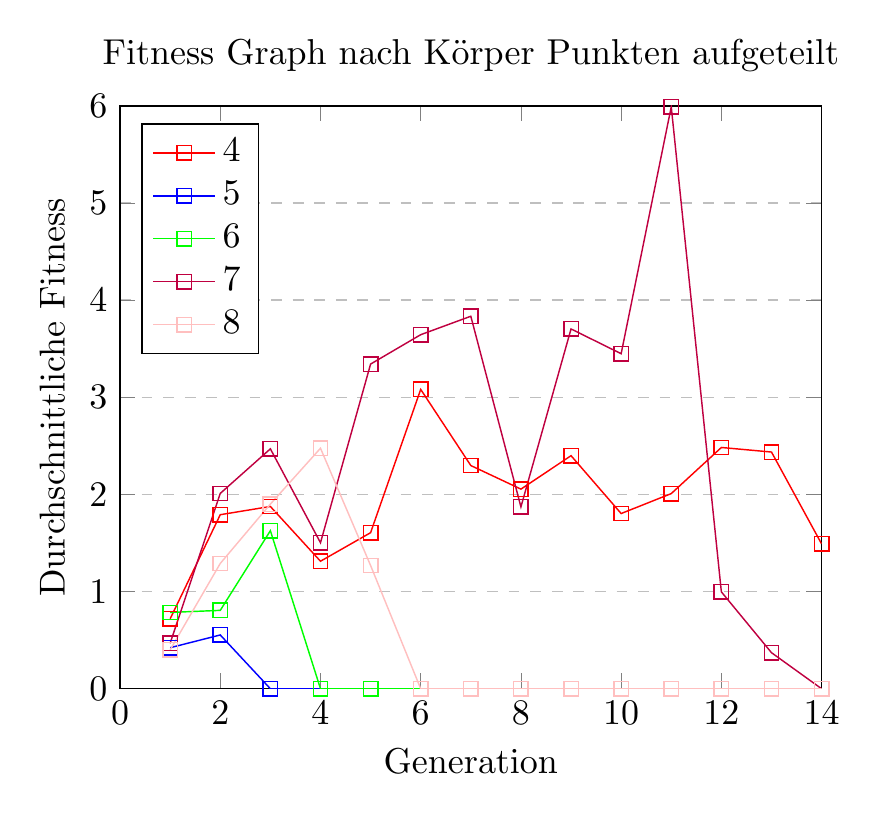
\begin{tikzpicture}[scale=1.3]
\begin{axis}[
    title={Fitness Graph nach Körper Punkten aufgeteilt},
    xlabel={Generation},
    ylabel={Durchschnittliche Fitness},
    xmin=0, xmax=14,
    ymin=0, ymax=6,
    xtick={0,2,4,6,8,10,12,14},
    ytick={0,1,2,3,4,5,6},
    legend pos=north west,
    ymajorgrids=true,
    grid style=dashed,
]

\addplot[
    color=red,
    mark=square,
    ]
    coordinates {
		(1,0.7197311288090767)(2,1.7917008390932372)(3,1.8763654203641982)(4,1.3127839017887504)(5,1.606485315324629)(6,3.081845732380266)(7,2.297797014315923)(8,2.055005581999147)(9,2.3994162926548404)(10,1.8036576432900295)(11,2.009064516425133)(12,2.4837885438165532)(13,2.436803859690654)(14,1.4910241046299537)
    };
    \addlegendentry{4}


\addplot[
    color=blue,
    mark=square,
    ]
    coordinates {
	(1,0.42241279780864716)(2,0.5535280124137276)(3,0)(4,0)(5,0)(6,0)(7,0)(8,0)(9,0)(10,0)(11,0)(12,0)(13,0)(14,0)
    };
    \addlegendentry{5}


\addplot[
    color=green,
    mark=square,
    ]
    coordinates {
	(1,0.7854441017622039)(2,0.8068950995802879)(3,1.6271000623703002)(4,0)(5,0)(6,0)(7,0)(8,0)(9,0)(10,0)(11,0)(12,0)(13,0)(14,0)
    };
    \addlegendentry{6}

\addplot[
    color=purple,
    mark=square,
    ]
    coordinates {
		(1,0.4685424281464469)(2,2.0108517235517502)(3,2.4697639744947937)(4,1.503244884001712)(5,3.3424592366328043)(6,3.644894652227138)(7,3.8348696411420136)(8,1.871792603770028)(9,3.70393052816391)(10,3.4490561534961066)(11,5.99130117893219)(12,0.9973328045823358)(13,0.37121231853961945)(14,0)
	};
    \addlegendentry{7}

\addplot[
    color=pink,
    mark=square,
    ]
    coordinates {
		(1,0.4001652509683654)(2,1.2898510225117206)(3,1.9010943668809803)(4,2.4758530855178833)(5,1.268694241841634)(6,0)(7,0)(8,0)(9,0)(10,0)(11,0)(12,0)(13,0)(14,0)
    };
    \addlegendentry{8}

\end{axis}
\end{tikzpicture}

          \caption{Durchschnittliches Individuum pro Anzahl Körperpunkte, Zweiter Versuch\label{fig:graphBpSecond}}
        \end{figure}

    \section{Dritter Versuch, parametrisierbare Steuerung ohne Feedback}

      \subsection{Konfiguration}

        \begin{table}[H]
          % !TEX root = ../main.tex

\begin{tabular}{ | l | l | }

  \hline
  \multicolumn{2}{|c|}{Simulationsparameter} \\
  \hline
  Populationsgrösse & 120 \\ \hline
  Selektionsstrategie & Turnierseletkion \\ \hline
  Iterationen & ca. 1200 \\ \hline
  Iterationsdauer & 30s \\ \hline
  Schwierigkeit erhöhen pro & 100 Generationen \\ \hline
  Steigungszuwachs & 0.01 \\ \hline
  Maximale Steigung & 1.0 \\ \hline
  Höchste Y-Koordinate Zuwachs  & 0.02 \\ \hline
  Ziel & Allgemeine Lösung \\ \hline
  \multicolumn{2}{|l|}{Wahrscheinlichkeit Mutation}\\ \hline
  \multicolumn{1}{|c|}{Allgemein} & 0.05 \\ \hline
  Engine &  \\ \hline
  \multicolumn{1}{|c|}{add} & 0.005 \\ \hline
  \multicolumn{1}{|c|}{remove} & 0.001 \\ \hline
  \multicolumn{1}{|c|}{lens} & 0.01 \\ \hline
  \multicolumn{1}{|c|}{id} & 0.001 \\ \hline
  \multicolumn{1}{|c|}{parameter} & 0.5 \\ \hline

\end{tabular}

          \caption{Simulationsparameter, Dritter Versuch}
        \end{table}

      \subsection{Auswertung}

        Leider dauert es mit dieser Version der Applikation sehr lange eine Generation zu evolvieren.
        Darum beschränkt sich dieser Versuch nur auf xxxx Generationen, damit Performance Optimierungen implementiert werden können.
        Die Individuen haben bei diesem Versuch, eine Art rollende Bewegung entwickelt.
        Sie können die guten Fitnesswerte halten, obwohl der Parcour immer schwerer wird (siehe Abbildung~\vref{fig:graphThird}).

        \begin{figure}
          % !TEX root = ../main.tex

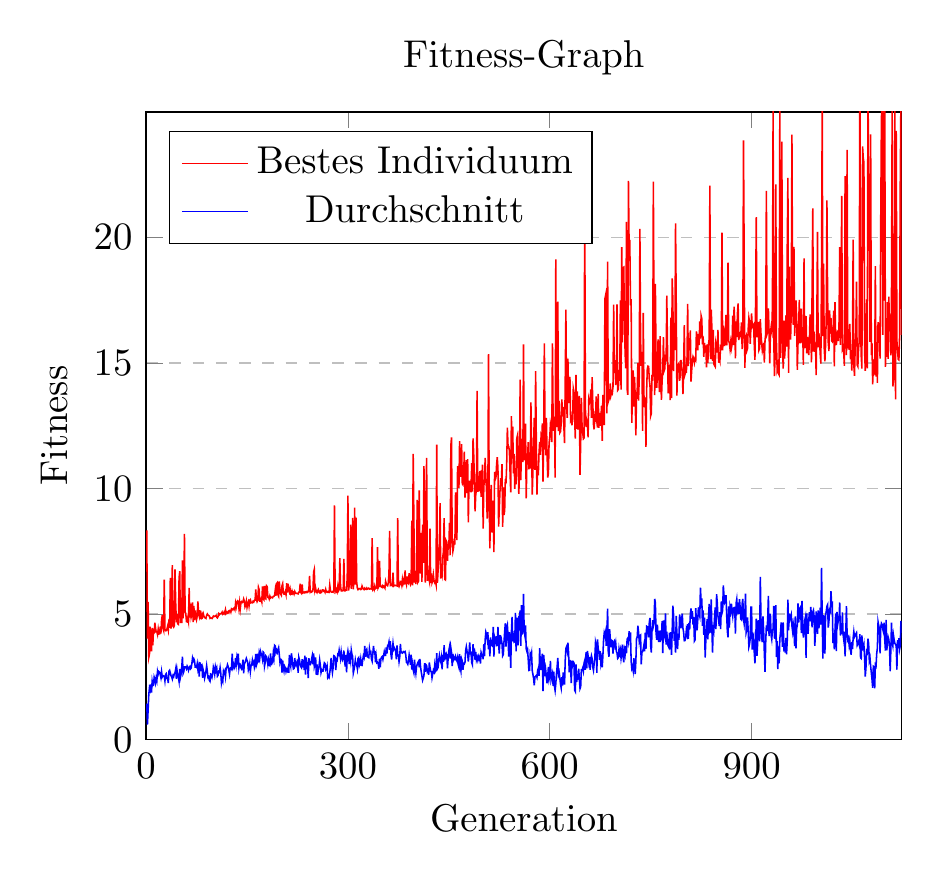
\begin{tikzpicture}[scale=1.4]
\begin{axis}[
    title={Fitness-Graph},
    xlabel={Generation},
    ylabel={Fitness},
    xmin=0, xmax=1123,
    ymin=0, ymax=25,
    xtick={0,300,600,900},
    ytick={0,5,10,15,20},
    legend pos=north west,
    ymajorgrids=true,
    grid style=dashed,
]

\addplot[
    color=red,
    mark=none,
    ]
    coordinates {
		(1,8.337641716003418)(2,4.0184645652771)(3,5.487634658813477)(4,3.268771171569824)(5,3.3982250690460205)(6,4.499021053314209)(7,3.691309928894043)(8,3.515028476715088)(9,4.444721698760986)(10,3.7522518634796143)(11,4.416717052459717)(12,4.221019744873047)(13,4.656446933746338)(14,4.452321529388428)(15,4.2899699211120605)(16,4.296048641204834)(17,4.185706615447998)(18,4.400793552398682)(19,4.207111358642578)(20,4.209735870361328)(21,4.4978742599487305)(22,4.218533992767334)(23,4.752462863922119)(24,4.955465316772461)(25,4.439781188964844)(26,4.3493852615356445)(27,6.367150783538818)(28,4.399297714233398)(29,4.336409568786621)(30,4.342099666595459)(31,4.4020256996154785)(32,4.515952110290527)(33,4.368217468261719)(34,4.791326522827148)(35,4.45461893081665)(36,6.443696022033691)(37,4.419928550720215)(38,5.808598518371582)(39,6.948536396026611)(40,4.520549297332764)(41,4.478343486785889)(42,4.533632755279541)(43,6.775493621826172)(44,5.4502081871032715)(45,4.674271583557129)(46,4.994293212890625)(47,4.611711502075195)(48,4.591427326202393)(49,6.427005290985107)(50,6.705092906951904)(51,4.635998725891113)(52,5.231718063354492)(53,4.6404242515563965)(54,7.138228416442871)(55,4.83296537399292)(56,5.4575300216674805)(57,8.198183059692383)(58,5.079111099243164)(59,5.0220746994018555)(60,4.698448181152344)(61,4.68707799911499)(62,4.85097074508667)(63,4.704654216766357)(64,6.040665149688721)(65,4.855485439300537)(66,5.410482883453369)(67,4.8824262619018555)(68,5.001476764678955)(69,5.468139171600342)(70,4.679938316345215)(71,5.3241658210754395)(72,4.756335735321045)(73,5.14747428894043)(74,4.917906761169434)(75,4.781447410583496)(76,4.917176723480225)(77,5.501983642578125)(78,5.0390305519104)(79,4.915684700012207)(80,5.1493611335754395)(81,4.827454090118408)(82,4.818329811096191)(83,5.000281810760498)(84,4.9070868492126465)(85,5.01362419128418)(86,4.908276081085205)(87,4.85512638092041)(88,4.851202964782715)(89,4.827971935272217)(90,4.951343059539795)(91,5.004500865936279)(92,4.960535526275635)(93,4.944637298583984)(94,4.923300266265869)(95,4.832083702087402)(96,4.853445529937744)(97,4.840818881988525)(98,4.823878765106201)(99,4.86625337600708)(100,4.92139196395874)(101,4.902008533477783)(102,4.914008617401123)(103,4.9282917976379395)(104,4.9483466148376465)(105,4.872841835021973)(106,4.846538066864014)(107,4.901675701141357)(108,5.014965057373047)(109,4.977746486663818)(110,5.01361608505249)(111,5.017216682434082)(112,5.0269775390625)(113,5.077807426452637)(114,4.990851402282715)(115,5.013479709625244)(116,5.076681137084961)(117,5.024285316467285)(118,5.172077655792236)(119,5.035671234130859)(120,5.077672481536865)(121,5.042375087738037)(122,5.095099925994873)(123,5.052812576293945)(124,5.150252819061279)(125,5.150534152984619)(126,5.077566146850586)(127,5.214122772216797)(128,5.196901798248291)(129,5.164315700531006)(130,5.227552890777588)(131,5.2450151443481445)(132,5.174229145050049)(133,5.4344987869262695)(134,5.295436382293701)(135,5.478116989135742)(136,5.527557849884033)(137,5.5007805824279785)(138,5.2363386154174805)(139,5.471573829650879)(140,5.216929912567139)(141,5.459837913513184)(142,5.496150970458984)(143,5.460948467254639)(144,5.491139888763428)(145,5.602490425109863)(146,5.509171485900879)(147,5.28665018081665)(148,5.3470048904418945)(149,5.5070905685424805)(150,5.271644115447998)(151,5.4166717529296875)(152,5.492286205291748)(153,5.319854259490967)(154,5.547508239746094)(155,5.576730728149414)(156,5.448465347290039)(157,5.455822467803955)(158,5.449313163757324)(159,5.506827354431152)(160,5.482302188873291)(161,5.550088405609131)(162,5.551332473754883)(163,5.984519958496094)(164,5.584130764007568)(165,5.491419792175293)(166,5.5435709953308105)(167,6.066195964813232)(168,5.98124361038208)(169,5.514509201049805)(170,5.510713577270508)(171,5.593795299530029)(172,5.482753276824951)(173,6.105553150177002)(174,5.609029293060303)(175,5.573231220245361)(176,6.12153434753418)(177,5.620379447937012)(178,5.6034255027771)(179,6.12676477432251)(180,6.093432426452637)(181,5.665706157684326)(182,5.667459011077881)(183,5.59725284576416)(184,5.7189412117004395)(185,5.645261287689209)(186,5.671420574188232)(187,5.666311740875244)(188,5.6499433517456055)(189,5.705088138580322)(190,5.703743934631348)(191,5.750663757324219)(192,5.96174430847168)(193,5.727972030639648)(194,6.212698459625244)(195,6.248234748840332)(196,5.763514041900635)(197,5.708507537841797)(198,6.303860187530518)(199,5.936214923858643)(200,5.7999587059021)(201,5.750758647918701)(202,6.127094268798828)(203,6.209222793579102)(204,5.8486833572387695)(205,5.795762538909912)(206,5.79394006729126)(207,5.8914947509765625)(208,5.774281978607178)(209,6.22984504699707)(210,5.854926109313965)(211,6.2078657150268555)(212,5.992016315460205)(213,5.8830885887146)(214,5.998076915740967)(215,5.783575057983398)(216,5.796772480010986)(217,5.919125080108643)(218,5.821643352508545)(219,5.865200519561768)(220,5.794439315795898)(221,5.899688243865967)(222,5.835334300994873)(223,5.820164680480957)(224,5.827912330627441)(225,5.819459438323975)(226,5.805851459503174)(227,5.873042583465576)(228,5.873746395111084)(229,6.211477279663086)(230,5.8588433265686035)(231,5.82452392578125)(232,6.179264068603516)(233,5.839381694793701)(234,5.849844932556152)(235,5.880352020263672)(236,5.848284721374512)(237,5.880436897277832)(238,5.861535549163818)(239,5.894623279571533)(240,5.868905067443848)(241,5.890384197235107)(242,6.002275466918945)(243,6.515683174133301)(244,5.878510475158691)(245,5.917879104614258)(246,5.879128932952881)(247,5.8981523513793945)(248,5.924780368804932)(249,6.6742777824401855)(250,6.779207706451416)(251,5.9349212646484375)(252,6.0362162590026855)(253,5.88839054107666)(254,5.852389812469482)(255,5.933241844177246)(256,5.981642723083496)(257,5.868082046508789)(258,5.849206924438477)(259,5.914815902709961)(260,5.854424476623535)(261,5.873373985290527)(262,5.9650559425354)(263,5.962552547454834)(264,5.912094593048096)(265,5.928625106811523)(266,5.866553783416748)(267,5.982507228851318)(268,5.880831241607666)(269,5.870488166809082)(270,5.895179271697998)(271,5.86417293548584)(272,5.861905574798584)(273,6.161482810974121)(274,5.94422721862793)(275,5.879997730255127)(276,5.875472068786621)(277,5.872368812561035)(278,5.908031463623047)(279,5.87587833404541)(280,9.331642150878906)(281,5.983882427215576)(282,5.896463871002197)(283,5.982696533203125)(284,5.898351669311523)(285,6.109954833984375)(286,5.924178123474121)(287,5.972482681274414)(288,7.226958751678467)(289,6.114979267120361)(290,5.927273273468018)(291,5.92030668258667)(292,5.923462390899658)(293,5.962270736694336)(294,7.198757648468018)(295,5.927533149719238)(296,5.928490161895752)(297,5.958340644836426)(298,5.953225612640381)(299,6.483359336853027)(300,9.712859153747559)(301,5.938929557800293)(302,6.169693470001221)(303,6.525606632232666)(304,8.560317039489746)(305,6.005934238433838)(306,6.646755695343018)(307,8.832021713256836)(308,5.9822468757629395)(309,6.478204250335693)(310,9.234922409057617)(311,6.176197528839111)(312,8.843140602111816)(313,6.284359455108643)(314,6.0345845222473145)(315,5.975447177886963)(316,6.0107550621032715)(317,6.008316993713379)(318,6.0171027183532715)(319,5.976761341094971)(320,5.986345291137695)(321,6.1153364181518555)(322,6.039125919342041)(323,6.004708290100098)(324,5.9759697914123535)(325,6.032904148101807)(326,5.998688697814941)(327,5.985610008239746)(328,6.038085460662842)(329,5.995763301849365)(330,6.0096049308776855)(331,6.030975341796875)(332,5.996053695678711)(333,5.999397277832031)(334,6.007864952087402)(335,5.998436450958252)(336,8.02116584777832)(337,5.984915733337402)(338,6.032752990722656)(339,5.966975212097168)(340,6.1228928565979)(341,6.0206732749938965)(342,6.046128273010254)(343,6.040995121002197)(344,7.668386936187744)(345,6.052603721618652)(346,6.111850261688232)(347,7.120563507080078)(348,6.104676723480225)(349,6.097665309906006)(350,6.0761823654174805)(351,6.128442764282227)(352,6.0666704177856445)(353,6.116689205169678)(354,6.087969779968262)(355,6.0356669425964355)(356,6.304139137268066)(357,6.2051920890808105)(358,6.147895812988281)(359,6.127424716949463)(360,6.245117664337158)(361,6.601839065551758)(362,8.316102027893066)(363,6.13275146484375)(364,6.138503551483154)(365,6.1789984703063965)(366,6.142375469207764)(367,6.64583683013916)(368,6.1160969734191895)(369,6.1396965980529785)(370,6.147129058837891)(371,6.137656211853027)(372,6.132750511169434)(373,6.122639179229736)(374,8.823402404785156)(375,6.148833751678467)(376,6.093331813812256)(377,6.163819313049316)(378,6.296420097351074)(379,6.284384250640869)(380,6.1558732986450195)(381,6.391622066497803)(382,6.2254638671875)(383,6.348618507385254)(384,6.173797607421875)(385,6.742833137512207)(386,6.2859673500061035)(387,6.17417573928833)(388,6.4993414878845215)(389,6.259109020233154)(390,6.219954490661621)(391,6.631834506988525)(392,6.298503875732422)(393,6.202667713165283)(394,6.358299732208252)(395,8.720865249633789)(396,6.144345760345459)(397,11.381012916564941)(398,8.887557983398438)(399,6.256819248199463)(400,6.458901405334473)(401,6.191874980926514)(402,6.737107276916504)(403,9.544281959533691)(404,6.266107559204102)(405,6.316109657287598)(406,9.928303718566895)(407,6.791256427764893)(408,6.615273952484131)(409,8.236763000488281)(410,6.283973693847656)(411,8.567084312438965)(412,7.043710231781006)(413,10.895868301391602)(414,8.543363571166992)(415,6.257015228271484)(416,9.55417537689209)(417,11.219818115234375)(418,6.32145881652832)(419,6.6287841796875)(420,6.460313320159912)(421,6.323060035705566)(422,8.40581226348877)(423,6.231586456298828)(424,6.614081382751465)(425,6.247429847717285)(426,6.335134506225586)(427,6.563512802124023)(428,6.3099188804626465)(429,6.247495651245117)(430,6.307552814483643)(431,6.177356719970703)(432,11.753419876098633)(433,6.245326995849609)(434,6.716487884521484)(435,7.1390862464904785)(436,7.943373680114746)(437,9.416289329528809)(438,6.413801670074463)(439,6.742499828338623)(440,6.591031551361084)(441,7.2711358070373535)(442,7.491066932678223)(443,8.823219299316406)(444,6.385529041290283)(445,6.361673355102539)(446,7.923859596252441)(447,7.864811897277832)(448,7.124953746795654)(449,7.718211650848389)(450,7.679666519165039)(451,8.631969451904297)(452,7.343308448791504)(453,11.720011711120605)(454,12.033319473266602)(455,7.852997779846191)(456,7.497190475463867)(457,7.639498710632324)(458,8.003934860229492)(459,7.76599645614624)(460,9.8501615524292)(461,9.07846450805664)(462,7.948515892028809)(463,10.895465850830078)(464,10.560994148254395)(465,10.025009155273438)(466,11.8927640914917)(467,10.46627426147461)(468,10.622767448425293)(469,11.773374557495117)(470,10.187896728515625)(471,10.150663375854492)(472,10.495702743530273)(473,11.472249031066895)(474,9.635607719421387)(475,10.105985641479492)(476,11.132173538208008)(477,9.817951202392578)(478,11.173310279846191)(479,8.649094581604004)(480,10.314362525939941)(481,9.881608963012695)(482,10.100751876831055)(483,9.85138988494873)(484,11.014360427856445)(485,9.881974220275879)(486,11.997859001159668)(487,11.353585243225098)(488,10.389106750488281)(489,9.08838176727295)(490,9.75267505645752)(491,9.946430206298828)(492,13.893165588378906)(493,9.872443199157715)(494,10.507830619812012)(495,9.887391090393066)(496,10.665759086608887)(497,10.676892280578613)(498,9.665061950683594)(499,10.229191780090332)(500,10.956282615661621)(501,8.406309127807617)(502,10.094558715820312)(503,10.308785438537598)(504,11.219680786132812)(505,10.5119047164917)(506,9.899886131286621)(507,8.799631118774414)(508,9.473828315734863)(509,15.350695610046387)(510,9.605722427368164)(511,7.621309280395508)(512,9.557476997375488)(513,10.14732837677002)(514,8.250448226928711)(515,8.471990585327148)(516,9.514994621276855)(517,7.46364164352417)(518,10.662060737609863)(519,10.36086654663086)(520,10.430702209472656)(521,10.962834358215332)(522,11.244498252868652)(523,10.808643341064453)(524,8.48244571685791)(525,9.197649955749512)(526,9.881793975830078)(527,10.414412498474121)(528,10.12694263458252)(529,10.974458694458008)(530,8.474931716918945)(531,10.041888236999512)(532,8.948553085327148)(533,9.125262260437012)(534,10.388158798217773)(535,10.203831672668457)(536,10.96680736541748)(537,12.421212196350098)(538,11.699240684509277)(539,11.678580284118652)(540,11.504353523254395)(541,10.633057594299316)(542,9.843705177307129)(543,12.880253791809082)(544,11.194149017333984)(545,12.46596908569336)(546,10.601951599121094)(547,11.37965202331543)(548,9.988120079040527)(549,10.813209533691406)(550,10.16409969329834)(551,12.00001335144043)(552,12.108620643615723)(553,11.104337692260742)(554,9.78674602508545)(555,10.62694263458252)(556,14.337990760803223)(557,10.332179069519043)(558,11.839805603027344)(559,11.917978286743164)(560,11.049240112304688)(561,15.740185737609863)(562,11.1229248046875)(563,12.266275405883789)(564,12.582237243652344)(565,9.605339050292969)(566,11.057835578918457)(567,11.177360534667969)(568,11.845305442810059)(569,10.764891624450684)(570,10.979349136352539)(571,10.795829772949219)(572,13.429532051086426)(573,11.738264083862305)(574,9.75357437133789)(575,10.705971717834473)(576,11.803427696228027)(577,12.809099197387695)(578,10.741613388061523)(579,14.672120094299316)(580,11.979580879211426)(581,9.761622428894043)(582,10.895533561706543)(583,10.528770446777344)(584,11.372077941894531)(585,11.856425285339355)(586,11.337483406066895)(587,12.009407043457031)(588,11.851785659790039)(589,12.593582153320312)(590,10.276772499084473)(591,12.147674560546875)(592,15.78609561920166)(593,12.211490631103516)(594,11.318446159362793)(595,12.816551208496094)(596,11.380187034606934)(597,10.435059547424316)(598,10.610873222351074)(599,11.812215805053711)(600,12.035940170288086)(601,12.553868293762207)(602,12.393935203552246)(603,11.84714412689209)(604,15.786105155944824)(605,12.765387535095215)(606,12.295071601867676)(607,12.859504699707031)(608,10.435474395751953)(609,19.130868911743164)(610,12.44633960723877)(611,12.881175994873047)(612,17.449438095092773)(613,12.29190444946289)(614,13.494592666625977)(615,12.221550941467285)(616,12.269068717956543)(617,12.572835922241211)(618,13.546876907348633)(619,12.879454612731934)(620,13.24911880493164)(621,12.445784568786621)(622,11.809772491455078)(623,14.234458923339844)(624,17.128246307373047)(625,13.2974853515625)(626,12.817977905273438)(627,15.173672676086426)(628,13.740854263305664)(629,13.403345108032227)(630,14.448265075683594)(631,12.728260040283203)(632,12.800707817077637)(633,12.521868705749512)(634,12.814543724060059)(635,13.993440628051758)(636,13.854349136352539)(637,12.805520057678223)(638,11.987524032592773)(639,14.524024963378906)(640,12.37874984741211)(641,13.873872756958008)(642,12.348306655883789)(643,13.390318870544434)(644,13.687944412231445)(645,10.546338081359863)(646,11.83608341217041)(647,13.609733581542969)(648,12.521965980529785)(649,12.216780662536621)(650,11.982443809509277)(651,12.016454696655273)(652,21.52263641357422)(653,13.191690444946289)(654,12.452725410461426)(655,12.70211410522461)(656,12.569183349609375)(657,12.041511535644531)(658,13.545388221740723)(659,13.410118103027344)(660,13.495165824890137)(661,13.946102142333984)(662,12.811720848083496)(663,14.438326835632324)(664,13.403158187866211)(665,12.551753044128418)(666,12.355093002319336)(667,12.821682929992676)(668,12.655981063842773)(669,13.667499542236328)(670,12.657811164855957)(671,12.42665958404541)(672,13.76744270324707)(673,12.414911270141602)(674,13.008515357971191)(675,12.49912166595459)(676,12.758234024047852)(677,13.300078392028809)(678,11.895895004272461)(679,13.732287406921387)(680,13.504582405090332)(681,12.529562950134277)(682,17.555883407592773)(683,17.68995475769043)(684,14.831342697143555)(685,12.989914894104004)(686,19.037742614746094)(687,13.459678649902344)(688,13.551830291748047)(689,13.613574981689453)(690,14.185062408447266)(691,13.723258018493652)(692,13.848760604858398)(693,13.796547889709473)(694,14.04462718963623)(695,17.321630477905273)(696,14.599445343017578)(697,15.112615585327148)(698,14.118462562561035)(699,14.617371559143066)(700,17.33296012878418)(701,13.91675853729248)(702,13.95689582824707)(703,14.722501754760742)(704,14.28674030303955)(705,17.492633819580078)(706,13.935425758361816)(707,19.61759376525879)(708,15.820049285888672)(709,18.797155380249023)(710,18.81688690185547)(711,16.90828514099121)(712,15.408597946166992)(713,14.789905548095703)(714,20.62088966369629)(715,13.967487335205078)(716,13.732381820678711)(717,22.253368377685547)(718,19.499269485473633)(719,19.903200149536133)(720,17.294567108154297)(721,17.54410171508789)(722,12.61589527130127)(723,14.141013145446777)(724,14.707757949829102)(725,13.264033317565918)(726,14.44320011138916)(727,13.690934181213379)(728,12.116867065429688)(729,13.713753700256348)(730,13.896805763244629)(731,15.007745742797852)(732,13.501983642578125)(733,14.37324333190918)(734,20.343257904052734)(735,15.989080429077148)(736,14.888601303100586)(737,15.439072608947754)(738,12.293525695800781)(739,16.998727798461914)(740,13.735053062438965)(741,13.23335075378418)(742,13.625689506530762)(743,11.655915260314941)(744,13.899579048156738)(745,14.762616157531738)(746,14.875219345092773)(747,14.861174583435059)(748,14.322209358215332)(749,14.117695808410645)(750,12.89001178741455)(751,12.984481811523438)(752,14.529468536376953)(753,14.294950485229492)(754,22.223079681396484)(755,16.583982467651367)(756,13.724838256835938)(757,18.148401260375977)(758,15.149996757507324)(759,14.014505386352539)(760,14.521781921386719)(761,15.939119338989258)(762,14.653594017028809)(763,13.845129013061523)(764,16.07008934020996)(765,14.518941879272461)(766,13.532553672790527)(767,14.281267166137695)(768,14.717241287231445)(769,16.029455184936523)(770,14.687213897705078)(771,14.769811630249023)(772,15.330819129943848)(773,15.054826736450195)(774,17.6823787689209)(775,15.699328422546387)(776,13.793977737426758)(777,14.927489280700684)(778,14.742931365966797)(779,13.517706871032715)(780,16.80513572692871)(781,13.604636192321777)(782,18.37032127380371)(783,17.528095245361328)(784,14.681078910827637)(785,16.149690628051758)(786,15.51143741607666)(787,20.556896209716797)(788,17.392044067382812)(789,13.706050872802734)(790,14.83946704864502)(791,14.939262390136719)(792,14.987822532653809)(793,14.291227340698242)(794,14.504085540771484)(795,15.12553882598877)(796,14.776484489440918)(797,14.728206634521484)(798,13.762613296508789)(799,14.785649299621582)(800,16.511987686157227)(801,14.540836334228516)(802,14.63330078125)(803,14.633193969726562)(804,15.093789100646973)(805,17.357240676879883)(806,14.875019073486328)(807,15.962015151977539)(808,15.672727584838867)(809,16.294437408447266)(810,14.258255958557129)(811,14.715581893920898)(812,15.095990180969238)(813,15.254608154296875)(814,15.18607234954834)(815,15.010178565979004)(816,15.167162895202637)(817,15.112454414367676)(818,16.263046264648438)(819,15.883532524108887)(820,15.50489330291748)(821,16.155378341674805)(822,15.71647834777832)(823,16.66037368774414)(824,15.976778030395508)(825,16.883071899414062)(826,16.765644073486328)(827,15.74810791015625)(828,16.062015533447266)(829,15.246615409851074)(830,15.80415153503418)(831,15.419637680053711)(832,15.697975158691406)(833,14.831314086914062)(834,15.736610412597656)(835,15.004059791564941)(836,15.752942085266113)(837,15.96069622039795)(838,22.060712814331055)(839,15.150398254394531)(840,17.129343032836914)(841,16.40666961669922)(842,15.075349807739258)(843,16.32088851928711)(844,14.958089828491211)(845,14.9000244140625)(846,14.851774215698242)(847,15.806025505065918)(848,15.660978317260742)(849,15.412995338439941)(850,16.32326316833496)(851,15.011798858642578)(852,15.260771751403809)(853,15.115198135375977)(854,15.728132247924805)(855,15.504555702209473)(856,20.19776153564453)(857,15.506054878234863)(858,16.488473892211914)(859,16.256256103515625)(860,15.676587104797363)(861,16.170103073120117)(862,16.91322898864746)(863,15.698938369750977)(864,16.11931037902832)(865,18.994735717773438)(866,15.87725830078125)(867,15.799551963806152)(868,15.558858871459961)(869,15.82440185546875)(870,15.581077575683594)(871,15.73464584350586)(872,16.882343292236328)(873,15.711263656616211)(874,17.243715286254883)(875,16.628511428833008)(876,15.181331634521484)(877,16.65973663330078)(878,16.034839630126953)(879,16.98039436340332)(880,17.37567901611328)(881,15.9118070602417)(882,16.120250701904297)(883,16.18462562561035)(884,16.087453842163086)(885,16.62026023864746)(886,15.55885124206543)(887,16.049230575561523)(888,23.864830017089844)(889,19.156200408935547)(890,14.80601978302002)(891,15.977394104003906)(892,16.064834594726562)(893,15.493753433227539)(894,15.581564903259277)(895,16.36583137512207)(896,16.79546356201172)(897,16.61677360534668)(898,15.76761531829834)(899,16.394628524780273)(900,16.977102279663086)(901,16.438974380493164)(902,16.48591423034668)(903,16.530338287353516)(904,15.737847328186035)(905,15.128265380859375)(906,17.505599975585938)(907,20.812477111816406)(908,16.02594757080078)(909,16.305082321166992)(910,16.6348819732666)(911,15.513566970825195)(912,15.591757774353027)(913,16.74704933166504)(914,16.16061782836914)(915,15.778461456298828)(916,15.487920761108398)(917,15.615060806274414)(918,15.803433418273926)(919,15.012228965759277)(920,15.8975248336792)(921,16.16417121887207)(922,21.85502052307129)(923,16.15078353881836)(924,16.235706329345703)(925,17.170333862304688)(926,16.249528884887695)(927,14.988199234008789)(928,16.17699432373047)(929,16.412704467773438)(930,16.273685455322266)(931,17.264623641967773)(932,25.13562774658203)(933,15.971452713012695)(934,14.479177474975586)(935,15.294669151306152)(936,22.110733032226562)(937,15.804564476013184)(938,14.758651733398438)(939,14.907369613647461)(940,14.581833839416504)(941,14.527998924255371)(942,25.187713623046875)(943,15.209573745727539)(944,17.248685836791992)(945,23.81985855102539)(946,15.780562400817871)(947,14.773159980773926)(948,16.69244956970215)(949,15.171592712402344)(950,15.6187162399292)(951,16.89236068725586)(952,15.649706840515137)(953,19.54820442199707)(954,22.376176834106445)(955,14.611660957336426)(956,18.8342342376709)(957,16.502891540527344)(958,15.929694175720215)(959,17.11600112915039)(960,24.094758987426758)(961,17.363788604736328)(962,16.521991729736328)(963,19.622190475463867)(964,16.085241317749023)(965,16.84160804748535)(966,17.492162704467773)(967,16.794710159301758)(968,14.728360176086426)(969,15.77258014678955)(970,16.52113151550293)(971,17.51325035095215)(972,15.815454483032227)(973,15.812150001525879)(974,17.163042068481445)(975,15.810914039611816)(976,16.239498138427734)(977,14.924250602722168)(978,19.165233612060547)(979,15.592377662658691)(980,16.01264762878418)(981,16.868011474609375)(982,15.385257720947266)(983,16.040607452392578)(984,15.84909725189209)(985,15.319718360900879)(986,15.967841148376465)(987,16.934375762939453)(988,16.493946075439453)(989,15.027729988098145)(990,18.012676239013672)(991,21.15669822692871)(992,15.453804969787598)(993,16.253681182861328)(994,15.443765640258789)(995,15.82069206237793)(996,14.520870208740234)(997,16.717180252075195)(998,20.227909088134766)(999,15.62635326385498)(1000,16.184709548950195)(1001,15.917961120605469)(1002,15.361420631408691)(1003,14.980744361877441)(1004,18.886186599731445)(1005,25.208202362060547)(1006,16.066316604614258)(1007,18.95525360107422)(1008,15.587867736816406)(1009,15.067076683044434)(1010,15.716431617736816)(1011,16.813112258911133)(1012,21.473995208740234)(1013,17.75836944580078)(1014,15.80489730834961)(1015,15.477217674255371)(1016,17.09370994567871)(1017,16.168598175048828)(1018,16.80103302001953)(1019,15.886938095092773)(1020,15.85312271118164)(1021,16.075456619262695)(1022,17.087377548217773)(1023,14.866348266601562)(1024,17.425495147705078)(1025,15.918926239013672)(1026,15.710957527160645)(1027,16.085914611816406)(1028,16.297203063964844)(1029,15.87238883972168)(1030,16.622764587402344)(1031,19.620500564575195)(1032,15.72467041015625)(1033,17.50066375732422)(1034,21.656085968017578)(1035,15.555668830871582)(1036,15.631111145019531)(1037,15.376730918884277)(1038,14.887652397155762)(1039,22.442041397094727)(1040,16.5877685546875)(1041,15.313490867614746)(1042,23.49057388305664)(1043,15.742307662963867)(1044,15.86677074432373)(1045,15.527106285095215)(1046,16.5620174407959)(1047,15.290735244750977)(1048,15.37162971496582)(1049,14.696459770202637)(1050,15.688087463378906)(1051,19.91805648803711)(1052,14.920710563659668)(1053,14.48491096496582)(1054,15.610963821411133)(1055,16.253137588500977)(1056,18.24379539489746)(1057,14.919161796569824)(1058,14.861735343933105)(1059,15.537409782409668)(1060,15.879759788513184)(1061,27.55990219116211)(1062,16.44008445739746)(1063,15.266425132751465)(1064,14.779086112976074)(1065,23.623388290405273)(1066,23.168048858642578)(1067,22.986120223999023)(1068,15.490964889526367)(1069,14.690497398376465)(1070,16.42139434814453)(1071,17.53693389892578)(1072,14.785414695739746)(1073,26.3134822845459)(1074,22.281267166137695)(1075,21.208995819091797)(1076,15.837249755859375)(1077,24.108417510986328)(1078,15.312273025512695)(1079,15.781268119812012)(1080,14.145896911621094)(1081,15.138900756835938)(1082,14.557621002197266)(1083,14.607288360595703)(1084,18.86101722717285)(1085,14.459778785705566)(1086,15.82988452911377)(1087,14.20572566986084)(1088,16.62837791442871)(1089,15.996018409729004)(1090,16.60219383239746)(1091,15.17453670501709)(1092,20.72237777709961)(1093,24.72115707397461)(1094,25.543710708618164)(1095,16.116262435913086)(1096,25.163047790527344)(1097,17.4805850982666)(1098,25.24859619140625)(1099,14.8487548828125)(1100,16.140615463256836)(1101,15.241332054138184)(1102,17.42087173461914)(1103,15.164253234863281)(1104,17.647579193115234)(1105,16.55990219116211)(1106,16.448610305786133)(1107,15.300239562988281)(1108,17.796459197998047)(1109,25.461397171020508)(1110,14.065865516662598)(1111,14.337145805358887)(1112,15.31286907196045)(1113,25.27859115600586)(1114,13.556527137756348)(1115,24.248794555664062)(1116,15.89082145690918)(1117,15.494329452514648)(1118,15.14848518371582)(1119,15.124610900878906)(1120,16.048625946044922)(1121,22.123979568481445)(1122,25.5994873046875)(1123,16.12203598022461)
	};
	\addlegendentry{Bestes Individuum}


\addplot[
    color=blue,
    mark=none,
    ]
    coordinates {
		(1,1.432452864293009)(2,0.594683917076327)(3,1.1690185462435088)(4,1.7883710400899873)(5,2.063868992154797)(6,1.9749660221859813)(7,2.2009114709372324)(8,1.8728574762120842)(9,2.319769443416347)(10,2.1515395530499517)(11,2.170587356792142)(12,2.4891800039835896)(13,2.4048105208824078)(14,2.2592227028061944)(15,2.457340863222877)(16,2.3455379746854303)(17,2.7202822864055634)(18,2.6059305294106405)(19,2.705527950450778)(20,2.6785692723467944)(21,2.600094203464687)(22,2.47098881204923)(23,2.707311345823109)(24,2.495187811180949)(25,2.549242115393281)(26,2.5330869954700272)(27,2.5250381299915414)(28,2.334211475495249)(29,2.600030827258403)(30,2.630263192206621)(31,2.4347985236595076)(32,2.437835646762202)(33,2.2520126229152084)(34,2.72222466521586)(35,2.7599629919975994)(36,2.6557622980326414)(37,2.548566083672146)(38,2.501741433531667)(39,2.4119068484132486)(40,2.551710288793159)(41,2.5099289221068224)(42,2.629215244227089)(43,2.662403790668274)(44,2.811461097933352)(45,2.416619047774293)(46,2.756156762301301)(47,2.547530953337749)(48,2.4732456447090954)(49,2.314335839667668)(50,2.8177497550224264)(51,2.4773197940628355)(52,2.609349640707175)(53,2.868849518833061)(54,3.3006773801830906)(55,2.63097755809625)(56,2.69840334666272)(57,2.8932544678604852)(58,2.8968262306104102)(59,2.893141970705862)(60,2.8229974708209435)(61,2.930193281515191)(62,2.8750025727475683)(63,2.7644608075420063)(64,2.8748656591866166)(65,2.910099232693513)(66,2.815300183960547)(67,2.846587663299094)(68,3.0266757936216893)(69,3.2455192608137926)(70,3.137262089860936)(71,3.210904693727692)(72,3.137659924228986)(73,2.885824961339434)(74,2.8859821443523592)(75,2.8698382151002684)(76,3.0253139699809255)(77,2.79596012737602)(78,2.9239567504574855)(79,2.5146325435489416)(80,3.0810898220787446)(81,2.729894054370622)(82,2.972328477228681)(83,2.9863662242889406)(84,2.457048184486727)(85,2.758088666697343)(86,2.636415554955602)(87,2.447916821887096)(88,2.5822105262428523)(89,2.7323224184413752)(90,2.9394344491884112)(91,2.7270944863506883)(92,2.4705404971415796)(93,2.5023139231527844)(94,2.3601083320255083)(95,2.3197376497322693)(96,2.6093019098198664)(97,2.5937326233523588)(98,2.492340149109562)(99,2.63470974676311)(100,2.8934943267454702)(101,2.799276355467737)(102,2.6161145879576604)(103,2.8952567224701244)(104,2.755892052936057)(105,2.8471111014174917)(106,2.5270867322571577)(107,2.5674906984592476)(108,2.7098371425954)(109,2.6858372330665587)(110,2.8629266804084184)(111,2.650447566822792)(112,2.2545887573311725)(113,2.4051976778854924)(114,2.322748224142318)(115,2.7275744497776033)(116,2.647137286669264)(117,2.7271478259315094)(118,2.517705348863577)(119,2.846365975278119)(120,2.8690382077552687)(121,2.9872542198126513)(122,2.910352880259355)(123,2.758436589501798)(124,2.604392610055705)(125,2.839452774481227)(126,2.8633537468810877)(127,2.8148224214402338)(128,3.426373422332108)(129,2.8984754886012523)(130,2.986628853529692)(131,2.8458075213556486)(132,2.9095362936457)(133,3.2567094789817927)(134,3.005525934758286)(135,3.2790905995837725)(136,3.1315040511700016)(137,3.4253836210817097)(138,2.862188080729296)(139,3.025225480707983)(140,3.00551516249155)(141,2.8596478689364933)(142,2.8128199351020156)(143,2.8870441733859478)(144,3.1846762523055077)(145,2.6433303971095787)(146,3.0150799370991685)(147,3.0661056538112463)(148,3.145737129387756)(149,3.23634506931218)(150,3.154005242853115)(151,3.0819848871479434)(152,2.7760107730784513)(153,2.879321015998721)(154,3.0202123963584504)(155,2.715921379160136)(156,2.9424780290884276)(157,2.9710820495771864)(158,3.1687763238325717)(159,3.0371644855787356)(160,3.0986512505759793)(161,2.8740023299586026)(162,2.9858320115755004)(163,3.416600374815365)(164,2.960878767756124)(165,3.046588323575755)(166,3.4269258527395627)(167,3.065175093252522)(168,3.4111430107848717)(169,3.250217068505784)(170,3.517056685934464)(171,3.4208388316289833)(172,3.364961251740654)(173,3.20723684434779)(174,3.4899635130384317)(175,3.4592577702676257)(176,2.9228232767277706)(177,3.0680282403171684)(178,3.3313867348556716)(179,3.295095453434624)(180,3.1724455863858263)(181,2.9893471378600225)(182,3.1649129746636997)(183,2.965274867974222)(184,2.9434013124361322)(185,3.4369946632223827)(186,2.960958134072522)(187,3.165422618528828)(188,3.1034281123429537)(189,3.422130709091046)(190,3.2558650044258686)(191,3.7598287006490865)(192,3.732853094597037)(193,3.4704133220016957)(194,3.557585982955061)(195,3.4727975765476002)(196,3.582198797313807)(197,3.6608323849116764)(198,3.3798963859987756)(199,3.0772314032850168)(200,3.199902010678003)(201,3.1855421229110408)(202,2.6718947670732933)(203,3.155979227109765)(204,2.84605541509809)(205,2.7197882154180357)(206,2.91541747074419)(207,2.851906449192514)(208,2.702594484606137)(209,2.7924527074831227)(210,2.7381468500825576)(211,2.84792279243314)(212,2.657130872302999)(213,3.370110774853189)(214,3.0583045030750022)(215,2.9191947893472387)(216,3.43635437770281)(217,3.2397337282658554)(218,2.9800075768648338)(219,2.815634640927116)(220,2.836496485583484)(221,3.247700295892234)(222,2.9700034484267235)(223,3.027646002173424)(224,2.948698117863387)(225,3.192617351406564)(226,2.6583772936835883)(227,3.2736515082108477)(228,3.1690748828463255)(229,2.9851256697128217)(230,2.9094934747864802)(231,2.8647640941043693)(232,3.2004559588773795)(233,2.8832818676096696)(234,3.184993967010329)(235,2.7668982710068426)(236,3.340559007351597)(237,2.587424496592333)(238,3.2712359422817827)(239,3.035231131967157)(240,2.99770826624784)(241,2.449080547511888)(242,3.2401975036986794)(243,2.9998220116831362)(244,2.9874177978063625)(245,3.041604003744821)(246,3.202525841258466)(247,3.337940253069003)(248,2.9987066427711397)(249,3.435542338279386)(250,2.919077141870124)(251,3.0481986083400745)(252,3.2712918049966295)(253,2.579030611536776)(254,2.994481165893376)(255,2.572908939421177)(256,2.809780083860581)(257,2.9075172065524386)(258,3.167073448157559)(259,2.9658431612576046)(260,2.670373995497357)(261,2.7807357283464325)(262,2.73318408842509)(263,2.7327144241270918)(264,2.908698962382429)(265,3.0573322693196436)(266,3.0260615973422924)(267,2.784181149614354)(268,2.831402049997511)(269,2.936009958726451)(270,2.4677662777365184)(271,2.51236042836681)(272,2.4716509780536096)(273,2.6644160854630172)(274,2.8803616647802603)(275,3.2485279294584566)(276,2.8861279588192703)(277,2.6669535502791404)(278,2.8638587198220193)(279,3.340515020551781)(280,3.32578612556681)(281,3.2718781352664035)(282,2.771389520416657)(283,3.195617379605149)(284,3.1644441591575743)(285,3.40192539030686)(286,3.3766165776643904)(287,3.563963198258231)(288,3.398101124167442)(289,3.2242714459309356)(290,3.4839048095978797)(291,3.246044134783248)(292,3.171269702503923)(293,3.272296908684075)(294,3.546385439539639)(295,3.1549446095867704)(296,2.9081045209177927)(297,3.370753074483946)(298,2.680566658487078)(299,3.3568750725282976)(300,3.5291662748282153)(301,3.3408745996964475)(302,3.0121359635299694)(303,3.3082727822164695)(304,3.1267985505672793)(305,3.5644637478554313)(306,3.3878800727271785)(307,3.3220640522117417)(308,2.6537906042998656)(309,2.778735514964986)(310,2.9329084197680158)(311,3.162404349880914)(312,2.9939724655821918)(313,2.977719775044049)(314,2.827726712396058)(315,3.227683763803604)(316,3.263605537234495)(317,2.9426367059660454)(318,3.0200798616123694)(319,3.2117843247950075)(320,2.960272994171828)(321,2.9550188727832087)(322,3.1738832435881097)(323,3.336543390651544)(324,3.2685020045454922)(325,3.734270206404229)(326,3.295118825013439)(327,3.543582378483067)(328,3.593823392863851)(329,3.298379634646699)(330,3.2863767862785607)(331,3.2639597858767955)(332,3.620916758198291)(333,3.4480584312851232)(334,3.4821984713276226)(335,3.205834017445644)(336,3.122846799677548)(337,3.415740790156027)(338,3.7331542960988977)(339,3.4837183993464955)(340,3.4906520477185645)(341,3.083036179250727)(342,3.3132503997689735)(343,3.0577955779153854)(344,3.077459925816705)(345,3.0271322137676178)(346,2.8210040769151723)(347,3.218817876341442)(348,2.8760312154268224)(349,3.2124597202365597)(350,3.2804291948365667)(351,3.307000840284551)(352,3.1944506816216744)(353,3.3400834013630325)(354,3.4944487143307925)(355,3.353892659426977)(356,3.3551892273438475)(357,3.6724926003565392)(358,3.4305509029193977)(359,3.7559359443684417)(360,3.7571891262196004)(361,3.8866173582850023)(362,3.5763027986822027)(363,3.9228015777810166)(364,3.393496036281188)(365,3.1886239708711703)(366,3.5804623366643984)(367,3.835273487569551)(368,3.592342098678152)(369,3.6566874413751065)(370,3.6016311914194374)(371,3.520908090472221)(372,3.196953908823586)(373,3.7507715793171275)(374,3.389806374942418)(375,3.362614294389884)(376,3.1021093108691273)(377,3.2820828096165013)(378,3.814547382419308)(379,3.4687746698502453)(380,3.488464734621812)(381,3.447295746586557)(382,3.468793153141936)(383,3.5035917706477147)(384,3.476471738036101)(385,3.5015609668722996)(386,3.3688533312796305)(387,3.0817711424392957)(388,3.0517940752363453)(389,3.0015763275170078)(390,3.1540239436551927)(391,3.36892333937188)(392,3.194259517211079)(393,2.9787473525851964)(394,3.381056618973768)(395,2.785683316628759)(396,2.9940148184464004)(397,2.7744221163704426)(398,2.6642452745853613)(399,3.181511847799023)(400,2.8316690029460005)(401,2.6345678044095013)(402,2.9075803741812707)(403,2.99401007029616)(404,3.0704498515697196)(405,3.1171112693380563)(406,2.8801880691821378)(407,3.2131850774089497)(408,2.8797276177754005)(409,2.695961888304252)(410,2.5342894570657033)(411,2.3634134366332242)(412,2.4468574692029508)(413,2.5493553931514423)(414,3.0403603288034597)(415,2.70097848046571)(416,2.9802186100122827)(417,2.951610200541715)(418,2.7136436510055018)(419,2.76385292718187)(420,2.5789294982658855)(421,3.070647061041867)(422,2.8829222289146856)(423,2.725500019080937)(424,2.705224688226978)(425,2.460295798901158)(426,2.603122986977299)(427,2.7525951354919624)(428,2.6973654999087255)(429,2.966804659397652)(430,2.7332083890913053)(431,2.799740355927497)(432,3.441397484764457)(433,2.821217055261756)(434,2.8765010989717363)(435,3.1602637014196566)(436,3.348721884097904)(437,3.1771296853820483)(438,3.090987600463753)(439,3.2703203310724347)(440,2.7989208788300552)(441,3.3669658557201427)(442,3.094475509412587)(443,3.7572371510167915)(444,3.1565062285944196)(445,3.387975216843188)(446,3.4375302818293374)(447,3.36239096634381)(448,2.8383037297831226)(449,3.249936308587591)(450,3.543303206982091)(451,3.685811772973587)(452,3.223076194625658)(453,3.6581296187204617)(454,3.468618881807197)(455,2.9237523580280445)(456,3.416183075060447)(457,3.1876253241867136)(458,3.266615748743061)(459,3.214930986892432)(460,3.316552055518453)(461,3.2050211822711088)(462,3.135443701517458)(463,3.2661666971068675)(464,2.9782065966321776)(465,2.874714165367186)(466,3.4057358469814063)(467,2.9024407317551475)(468,2.7345978651971867)(469,3.210518979172533)(470,3.1269488143424193)(471,2.784741300996393)(472,3.03472270903488)(473,3.014859583817694)(474,3.079209236994696)(475,3.547103963792324)(476,3.6986469716760135)(477,3.527119367949975)(478,3.406950112308065)(479,3.1049896726074317)(480,3.4280952695165374)(481,3.8717368617032966)(482,3.437268852101018)(483,3.4576913880339513)(484,3.067935750198861)(485,2.9873695207759736)(486,3.8052352286467794)(487,3.329099221838017)(488,3.6284974301583133)(489,3.176280661770822)(490,3.4934432661160826)(491,3.1757336263932907)(492,3.275843662628904)(493,3.1600871892335514)(494,3.3141812422002355)(495,3.2285735161664584)(496,3.3042296962967765)(497,3.0287016799362996)(498,3.464313331649949)(499,3.3673993702046574)(500,3.374883260927163)(501,3.202588450505088)(502,3.7963971481348078)(503,3.3258936943486335)(504,3.97924992206196)(505,4.284060698808753)(506,4.193524589203298)(507,4.00781094605724)(508,4.280375156582644)(509,3.5991309863204757)(510,3.9667891334121426)(511,3.3150671684648843)(512,4.072336198358486)(513,3.7885163620890427)(514,3.756670487423738)(515,3.7265848910979305)(516,4.486631480728587)(517,3.310027911203603)(518,4.097778286164005)(519,3.9962157065980137)(520,3.8743873540622493)(521,4.121442564258662)(522,3.721567399512666)(523,4.491087730663518)(524,3.7978753421921283)(525,3.4263072168764968)(526,4.16344726588965)(527,3.912795898426945)(528,4.007251660618931)(529,3.8337809081499774)(530,3.335749222710729)(531,3.3909474471506353)(532,3.901713199525451)(533,4.301410594442859)(534,4.6325662069953975)(535,3.7023850423671925)(536,4.478515443392098)(537,4.574656025165071)(538,4.139367254557631)(539,3.303120657429099)(540,4.277576913944601)(541,3.827181030648838)(542,2.8577384830142063)(543,4.247920642032598)(544,4.8853688372143855)(545,3.914946958096698)(546,4.099604051311811)(547,3.8837441422666115)(548,3.9026168858942887)(549,5.051004126753347)(550,3.517802686135595)(551,4.612999262381345)(552,4.852923337207176)(553,3.7523262969994295)(554,4.853524555917829)(555,4.8188410887882736)(556,5.14840762684471)(557,3.7364978991836932)(558,5.355813848398005)(559,4.187358597109172)(560,4.469477472788033)(561,5.802969232853502)(562,4.29760265716662)(563,4.143885932055612)(564,4.551044286959708)(565,3.618316039070487)(566,3.5189316804831225)(567,3.594524151311877)(568,3.2054340839230764)(569,2.7552510862316315)(570,2.764351458948416)(571,3.3959099075601746)(572,3.2914533513753366)(573,3.4442130324741203)(574,2.743492490107504)(575,2.596196650993079)(576,2.439050928984458)(577,2.162756478530355)(578,2.4972678079580266)(579,2.5226884888795515)(580,2.552330013071575)(581,2.4779591834318127)(582,2.751515115640359)(583,2.839035832695663)(584,2.540313897343973)(585,3.645382876632114)(586,2.97175845229843)(587,2.771311446434508)(588,3.1686146521009504)(589,3.4208919321807723)(590,1.9348725997787066)(591,3.3740369353753823)(592,2.9881814093872285)(593,2.525413350512584)(594,2.774350483963887)(595,2.503527246788144)(596,2.2434880019941676)(597,2.5235332238177457)(598,2.897814293919752)(599,2.3984690562356263)(600,2.5331654384111366)(601,3.1343546364922075)(602,2.385802917415276)(603,2.5109839723367866)(604,2.6277609629246097)(605,2.145804239778469)(606,2.7017210541603465)(607,2.122912499199932)(608,1.9511263316846452)(609,2.2265908563509584)(610,2.6197037253839275)(611,2.913791560381651)(612,3.256897744544161)(613,2.5883262869281074)(614,2.6819860778438547)(615,2.45216198155346)(616,2.2008372431242607)(617,2.054435939900577)(618,2.4859878642251716)(619,2.149447856928843)(620,2.673202985494087)(621,2.3908134592076142)(622,2.1946767604599398)(623,3.1597593888174744)(624,3.6299921099096535)(625,3.69777267362612)(626,3.544526230668028)(627,3.858573156207179)(628,3.4602024873602204)(629,2.6756690836201114)(630,3.1701294077094646)(631,2.8947321332137412)(632,2.25237726730605)(633,3.140676448987021)(634,2.971564032132058)(635,3.0969534347988277)(636,3.062411961743298)(637,1.9643960643734317)(638,1.912341228798808)(639,2.9956824418157337)(640,2.2896135810005944)(641,2.485265533129374)(642,2.4533599114433553)(643,2.8275335527335606)(644,2.409549785948669)(645,2.033917601381351)(646,2.1090284663873415)(647,2.7766610622406005)(648,2.773162454304596)(649,2.854944824365278)(650,2.7255645020321633)(651,3.0458460888204475)(652,3.150367164988226)(653,2.7744292450447876)(654,3.4804448041754465)(655,2.839770287711872)(656,3.529527615833407)(657,3.3357693006594977)(658,3.090593660591791)(659,3.294831038452685)(660,2.783180638134945)(661,3.1763310340543587)(662,3.338613263765971)(663,3.222234436062475)(664,2.882217284416159)(665,2.757378212440138)(666,3.012009808254273)(667,3.2276580676281204)(668,3.868200820715477)(669,3.7289210816224414)(670,2.6591824495078376)(671,3.99025301374495)(672,3.6253068297596958)(673,3.505899255909026)(674,3.180631671473384)(675,3.5218746423721314)(676,3.0347190563489375)(677,3.1964345804338032)(678,2.8818249592664262)(679,3.345840162263873)(680,3.9703169642637173)(681,4.250103766160707)(682,4.137304273247719)(683,4.2818320561510825)(684,3.7316810339999695)(685,4.272146774409339)(686,5.21535910529395)(687,3.5050731918464106)(688,3.2998105926439165)(689,4.394771213953693)(690,4.026748680137098)(691,3.674635344122847)(692,3.9535511188209056)(693,3.93559073441041)(694,3.4264389076580604)(695,3.8462578054827947)(696,3.911435945231157)(697,3.73848661792775)(698,3.872710584104061)(699,3.515931284520775)(700,3.4488752016797664)(701,3.2345288963988423)(702,3.269239091128111)(703,3.610762465139851)(704,3.441288338477413)(705,3.569406488165259)(706,3.2401705072571834)(707,3.4382026908919214)(708,3.785754995032524)(709,3.310849024976293)(710,3.081818325103571)(711,3.5458379954565316)(712,3.39023353420198)(713,3.728149031785627)(714,3.433341111956785)(715,4.002165917803844)(716,4.042873837798834)(717,3.891838156928619)(718,4.3142886669375)(719,3.9388262117281556)(720,4.2732430743053555)(721,3.1158897624971966)(722,2.8323490478408835)(723,2.914590701336662)(724,2.7470214042191703)(725,3.240989195027699)(726,3.013184282804529)(727,2.613324137156208)(728,3.1191871146050594)(729,4.030122691594685)(730,4.07327562669913)(731,4.534052268850306)(732,4.284178442694246)(733,3.930074197550615)(734,4.1375660098157825)(735,4.163322788135459)(736,2.993215280212462)(737,3.485287600258986)(738,3.5006912555623177)(739,3.611550807409609)(740,3.7705159043272336)(741,3.5122342634480446)(742,4.257433242661258)(743,3.6123638304260868)(744,4.516236694680993)(745,4.49936011050983)(746,4.288109019740174)(747,4.070111697912216)(748,4.685385712577651)(749,4.846360536788901)(750,3.7443882738550505)(751,3.4693416505741577)(752,4.35710537272195)(753,4.7531799994098645)(754,4.512273853536074)(755,4.630579945445061)(756,5.605898340605199)(757,5.445335924873749)(758,4.259596948573987)(759,3.973865012824535)(760,4.575891735901435)(761,4.092918403819203)(762,3.8863307074798894)(763,4.339515128755011)(764,3.8872630072757604)(765,4.346086825088908)(766,3.9500118493412932)(767,4.713959279245076)(768,3.449878679464261)(769,4.745160725309203)(770,4.205478587211109)(771,4.095419081513925)(772,5.023588496105124)(773,3.7831083717445533)(774,4.300629198923707)(775,3.8114804431696636)(776,3.7286384483178456)(777,3.6725613734684885)(778,4.258408352383412)(779,3.5996164879451196)(780,4.283079929510132)(781,3.3749868489181)(782,4.336187593763073)(783,5.330918677647909)(784,4.994415561233958)(785,3.932916460558772)(786,4.222357766035324)(787,3.463897091837134)(788,4.9244940448241925)(789,4.2481904440249005)(790,3.604809395619668)(791,4.21502865695705)(792,3.976928203646094)(793,4.986375188299765)(794,4.8029346478482084)(795,4.4368484330984455)(796,4.793441830358158)(797,5.014740916838249)(798,4.434297518804669)(799,4.280440723864983)(800,3.938150923202435)(801,3.945392759454747)(802,4.041073798791816)(803,4.3504883796907965)(804,4.209059043849508)(805,4.598745787888765)(806,4.008595729262257)(807,4.64333209892114)(808,4.3873461469154185)(809,5.0120209127975)(810,5.221459727423887)(811,4.807108137508234)(812,5.120213181539051)(813,4.576936221697057)(814,4.881920077092945)(815,3.924729616070787)(816,3.969172902653615)(817,5.2401555704515586)(818,4.644926919865733)(819,4.353024244308472)(820,4.769856360368431)(821,5.26910070652763)(822,5.011296727285177)(823,4.900722958923628)(824,6.056468442703287)(825,5.4696222081392385)(826,5.622979576016466)(827,4.529776299698279)(828,5.141308592779873)(829,4.169259656624248)(830,4.8616008878995975)(831,3.270874433948969)(832,3.945963641128037)(833,4.384647921783229)(834,4.7931571429469235)(835,3.99055004104351)(836,4.889070385927335)(837,5.408177705365233)(838,4.277776858893533)(839,4.297870394711693)(840,5.585022059397306)(841,4.435896281812408)(842,3.464499949446569)(843,4.56445356781284)(844,4.384430368267931)(845,4.885702859734495)(846,5.26715314121296)(847,4.404281182476552)(848,5.788954009705534)(849,5.458084809252371)(850,4.919804194274669)(851,4.739648701405773)(852,4.527794358072182)(853,5.071437202797582)(854,4.39836449790746)(855,5.508998721465469)(856,5.033362322424849)(857,5.134725677592602)(858,6.139316703441242)(859,5.749275257601402)(860,5.448268233596658)(861,5.504136970592663)(862,5.752332191270155)(863,4.962208119826391)(864,4.309561379253864)(865,4.07121430117016)(866,5.307820517197252)(867,4.458959421546509)(868,5.272063225965637)(869,5.127010112286856)(870,5.415880566462874)(871,5.156105399162819)(872,4.925527083749572)(873,5.219696308800485)(874,5.25993420848002)(875,5.261836697782079)(876,4.224911067790042)(877,5.426446566234032)(878,5.592156137526035)(879,5.151945803609366)(880,5.276821456321826)(881,5.0006096619647)(882,5.59665941670537)(883,5.279204166059693)(884,4.804709408928951)(885,4.771561116457451)(886,5.425779207578549)(887,5.6058338007579245)(888,4.79324319063841)(889,4.609818359510973)(890,4.987426322946946)(891,5.810470433859154)(892,4.280885794789841)(893,4.421901533223293)(894,4.870150589785771)(895,4.341690099736055)(896,3.6950467716592055)(897,3.8138275225646794)(898,4.01881121667102)(899,5.276553930710846)(900,5.278295815363526)(901,3.5826666809172214)(902,4.072618624785294)(903,4.155051721089209)(904,3.4692771358182655)(905,3.03863727664575)(906,3.71583630690972)(907,4.816897481540218)(908,3.333869490950989)(909,3.8297261961798843)(910,4.758022812381387)(911,4.252145987811188)(912,3.9131391384638845)(913,6.476284960781535)(914,4.777554074053963)(915,4.04828898293199)(916,3.8806496816687286)(917,4.904078285613408)(918,4.298058890737593)(919,3.432501287960137)(920,2.6957472504271816)(921,3.8625598423493406)(922,4.548592524370179)(923,4.317687159016107)(924,4.848266007906447)(925,5.728730527932445)(926,4.120038122342279)(927,4.824332069884986)(928,5.011687263691177)(929,4.162184083337585)(930,3.993315569316231)(931,4.35351115656534)(932,4.412379252010336)(933,5.324978674234202)(934,4.053692786861211)(935,4.0349232159399735)(936,5.356958588041986)(937,3.29179229682001)(938,3.9190687904677666)(939,2.8056303905012707)(940,3.707580716939022)(941,3.032842700664575)(942,4.015743118555595)(943,4.270007459200375)(944,4.664789106448492)(945,4.248924680327764)(946,3.6993710760376417)(947,4.663403416859607)(948,3.6248893497162498)(949,3.6842901966534556)(950,3.464997721044347)(951,4.047685634655257)(952,3.3977398791971307)(953,3.9309968629231054)(954,5.575191507736842)(955,4.350795305633801)(956,5.020083955535665)(957,4.781664651663353)(958,4.87814086744717)(959,4.97792305527255)(960,4.5311326193623245)(961,4.318077047002347)(962,4.606670962211987)(963,4.413505514214436)(964,3.726344486263891)(965,4.9041613664478065)(966,3.6325266514128693)(967,4.421267358524104)(968,4.565054175459469)(969,5.421439824129144)(970,4.66031579185122)(971,4.988184602186084)(972,5.24891073256731)(973,5.2924130591874325)(974,4.2417493181303145)(975,5.521949545821796)(976,4.6017890690205)(977,4.0662247985601425)(978,4.288513360917568)(979,4.746546172067368)(980,4.874897524217764)(981,3.259706771746278)(982,5.022405451287826)(983,4.44553865455091)(984,4.214425353705883)(985,4.755396588922789)(986,5.078507835200678)(987,4.708147687961658)(988,5.287499076873064)(989,4.846154970489442)(990,4.474664342869073)(991,5.081133875945428)(992,5.15402313338127)(993,4.893521906559666)(994,3.7296173898503184)(995,4.316169645544141)(996,5.106373510944347)(997,4.429753404545287)(998,4.212884266239901)(999,5.146253944622973)(1000,4.429901697890212)(1001,4.674733502728244)(1002,5.25260668968161)(1003,4.583061422330017)(1004,6.834663343243301)(1005,4.8335498850870255)(1006,3.229769925090174)(1007,4.953379832642773)(1008,4.792419574533899)(1009,3.4234884293129046)(1010,4.942728049680591)(1011,5.110371411917731)(1012,5.314140955746795)(1013,5.371936056281751)(1014,4.4591720479850965)(1015,4.707169089776774)(1016,5.251670559961349)(1017,5.0157368815193575)(1018,5.909372532491883)(1019,5.381935757864267)(1020,5.419795423125227)(1021,3.8398055912305913)(1022,4.243569464267542)(1023,3.5992384983769927)(1024,4.336032843030989)(1025,5.028948876754536)(1026,3.528225658950396)(1027,5.083349975322684)(1028,4.589309047286709)(1029,4.752900825440884)(1030,4.752860617854943)(1031,5.459859144377211)(1032,4.14733639943103)(1033,4.635723409646501)(1034,4.196333995368332)(1035,5.065752358276708)(1036,4.193557219735037)(1037,3.983676453990241)(1038,4.294985059648752)(1039,3.3174143910097578)(1040,4.203244385123253)(1041,5.313328363304026)(1042,4.221587114548311)(1043,3.9758635122328996)(1044,4.048654849089993)(1045,3.7711351605442665)(1046,3.9421961879978578)(1047,3.594296914090713)(1048,3.37814478102761)(1049,3.8914080742591373)(1050,3.601758888658757)(1051,4.0416790716350075)(1052,4.298805990194281)(1053,4.089327095014354)(1054,4.146633866180976)(1055,4.206043842279663)(1056,4.254647930214802)(1057,3.7592656620467704)(1058,3.8237323156868417)(1059,3.904829160372416)(1060,3.784635381307453)(1061,4.201913152635098)(1062,3.2598652665813765)(1063,3.231885728985071)(1064,4.146970614014815)(1065,3.5812714270005626)(1066,3.5965546182667216)(1067,3.765199786548813)(1068,3.2524019524455072)(1069,2.51227918813626)(1070,2.850264216773212)(1071,3.507328006563087)(1072,3.4578891839599235)(1073,4.020835612582354)(1074,3.8245066843926905)(1075,3.1590323279766985)(1076,3.2638043937661374)(1077,2.9224861331303447)(1078,2.655783588765189)(1079,2.4013520484479765)(1080,2.06660998503988)(1081,2.918611272176107)(1082,2.8955293226987124)(1083,2.0398226376002033)(1084,2.9739257315173746)(1085,2.9262617068986096)(1086,3.4227776650339363)(1087,3.6491903685033322)(1088,4.692549078414838)(1089,4.544731187696258)(1090,4.412981104850769)(1091,3.4375250707690914)(1092,4.477611977172395)(1093,4.6346260080114)(1094,4.5862500929584105)(1095,4.389074067243685)(1096,4.288924879487604)(1097,4.653454428166151)(1098,3.9520257238298653)(1099,3.5408333824326594)(1100,4.763514591008425)(1101,3.558231157825018)(1102,3.833644922543317)(1103,4.085093841111909)(1104,3.9857095747875673)(1105,3.7723351549667616)(1106,2.7233909192495047)(1107,3.533344986041387)(1108,4.660695368982852)(1109,3.8682761875563303)(1110,3.7342485378923205)(1111,4.141387143358588)(1112,3.9604751134912175)(1113,3.8311096005762617)(1114,3.7915191154616577)(1115,3.73612751023223)(1116,2.7830228015392398)(1117,3.9591812355909495)(1118,3.6405614114056033)(1119,4.0365197037889935)(1120,3.5942091734536614)(1121,3.7337413522958136)(1122,4.730860172895094)(1123,4.250748832368602)
	};
    \addlegendentry{Durchschnitt}




\end{axis}
\end{tikzpicture}

          \caption{Bestes Individuum und Durchschnittliches Individuum, Dritter Versuch\label{fig:graphThird}}
        \end{figure}

        \subsubsection{Körperpunkte}

          Auf eine Diskussion der Körperpunkte wird verzichtet.
          Die notwendigen Schritte für eine sinvolle Evaluation wurden unter~\vref{subsub:bpScnd} beschrieben.

        \subsubsection{Diversität}
          Ab dieser Simulation ist endlich der Diversitätsreport verfügbar. Wie in~\vref{fig:graphDivThird} zu sehen ist,
          ist die Diversität kurz auf einem hohen Niveau, da am Anfang alles völlig zufällig generiert wird.
          Durch die nachfolgenden Selektionen sinkt sie, da mit hoher wahrscheinlichkeit nur leistungsstarke Individuen
          bei der Tunier-basierten Selektion gewinnen. Interessant zu beobachten ist,
          das die Diversität ab der 400. Generation wieder zu steigen beginnt.
          Die Vermutung dabei ist, dass sich immer mehr verschiedene Individuen mit einer
          guten Fitness finden lassen.

          \begin{figure}
            % !TEX root = ../main.tex
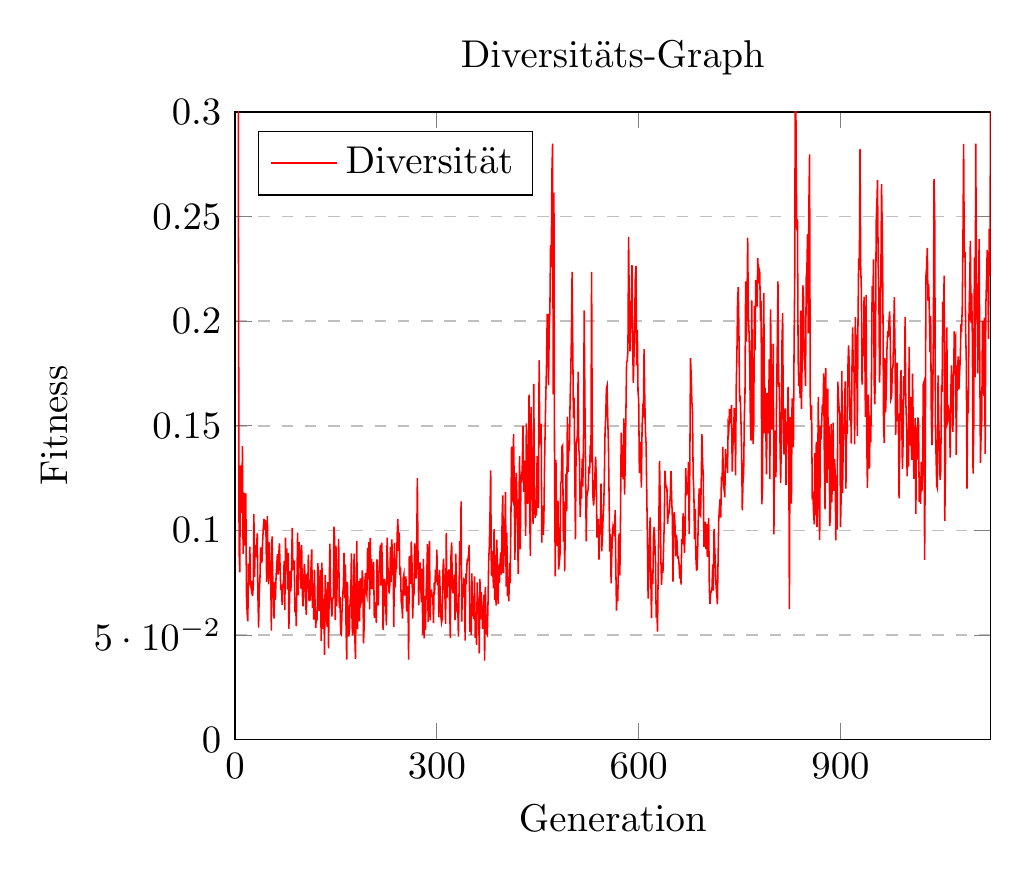
\begin{tikzpicture}[scale=1.4]
\begin{axis}[
    title={Diversitäts-Graph},
    xlabel={Generation},
    ylabel={Fitness},
    xmin=0, xmax=1123,
    ymin=0, ymax=0.3,
    xtick={0,300,600,900},
    ytick={0,0.05,0.1,0.15,0.2,0.25,0.3},
    legend pos=north west,
    ymajorgrids=true,
    grid style=dashed,
]

\addplot[
    color=red,
    mark=none,
    ]
    coordinates {
      (1,2.3965844354721564)(2,2.40895019902692)(3,2.535503478947583)(4,1.665492146667334)(5,0.25705991177976684)(6,0.09047587310012281)(7,0.07991030239339486)(8,0.1311073500539815)(9,0.11796192896267256)(10,0.10823481071672433)(11,0.1403127582405985)(12,0.08873189362773702)(13,0.11020758378856424)(14,0.11788916105188517)(15,0.09267230711283676)(16,0.11770484927238359)(17,0.06862103690972096)(18,0.060540153174981425)(19,0.05651529852079352)(20,0.08414115259230155)(21,0.07394708980129053)(22,0.09229157789011687)(23,0.07436260297300078)(24,0.07227046454670948)(25,0.07583220001988616)(26,0.06866732309272834)(27,0.07250865414395094)(28,0.10778808722791701)(29,0.07777383242045982)(30,0.09300756264348232)(31,0.08714148966153946)(32,0.09213314697262694)(33,0.09851551955275838)(34,0.06892416770350102)(35,0.05347728865441617)(36,0.0704629164053006)(37,0.07651880603915999)(38,0.09186248645255841)(39,0.08482333450188449)(40,0.0849360338210756)(41,0.09465793273380804)(42,0.10107732465429771)(43,0.10544346339757299)(44,0.10031784878359683)(45,0.10506082236651473)(46,0.09838339260434746)(47,0.0754489570843809)(48,0.10678511963944676)(49,0.08611963571418786)(50,0.0742477976835385)(51,0.09431948244346806)(52,0.08478473878581218)(53,0.0802160949912323)(54,0.052037668826280366)(55,0.09710511058595392)(56,0.07827595871905678)(57,0.0699681152379075)(58,0.05789021716198126)(59,0.07521130763047)(60,0.06683218863962291)(61,0.07794880739573316)(62,0.08342635486983568)(63,0.08864663038047298)(64,0.07884347872799428)(65,0.0885247685986539)(66,0.09383021340503381)(67,0.08196005178300325)(68,0.07144818420765689)(69,0.07409830088075646)(70,0.0644016854544252)(71,0.07387874424172146)(72,0.07512332249748986)(73,0.08542245051361005)(74,0.061900560600782334)(75,0.09653335223272205)(76,0.08049397826795154)(77,0.09144686749428149)(78,0.0717590260474288)(79,0.08928293433294596)(80,0.05299000571701931)(81,0.06623087722005024)(82,0.08052793391618736)(83,0.07102939324199911)(84,0.08239929456941791)(85,0.10121135853329757)(86,0.08163836519264772)(87,0.08212922104140025)(88,0.08558409324858841)(89,0.06077737482703663)(90,0.0679787702869367)(91,0.0542832651159028)(92,0.07543713064178653)(93,0.09895640176536077)(94,0.06895944297687087)(95,0.09442823290746676)(96,0.09151862631465041)(97,0.08704846119320954)(98,0.07215122221799887)(99,0.0930823632218241)(100,0.07031459064015193)(101,0.06365195824554735)(102,0.07346607460036204)(103,0.08398993720145549)(104,0.0784934736761191)(105,0.06462196223676088)(106,0.05949228665369681)(107,0.07925356512719758)(108,0.07204490718771721)(109,0.08844230093514158)(110,0.06609437286889004)(111,0.07101792511102957)(112,0.06644209484537987)(113,0.08346646003798144)(114,0.09090235891821027)(115,0.0629906418127246)(116,0.07477212059353865)(117,0.057399276971160075)(118,0.08126992391825913)(119,0.0637454221389481)(120,0.05338806314511537)(121,0.06107885703207432)(122,0.05687512829474639)(123,0.0843366789814623)(124,0.07863227989860797)(125,0.06150897178062098)(126,0.07102907838128823)(127,0.08097462780861037)(128,0.0471418893060825)(129,0.08456088586630965)(130,0.07294971642383863)(131,0.05294383827935458)(132,0.06741065717221488)(133,0.04046422148324392)(134,0.07872005580466786)(135,0.07084190082397755)(136,0.05792031905745628)(137,0.05378819505298812)(138,0.0752356906966037)(139,0.043570457575875306)(140,0.07348810673803435)(141,0.09368959109436734)(142,0.0688918942300028)(143,0.0652381957411075)(144,0.05884550276556187)(145,0.06757814754435344)(146,0.06774181080176804)(147,0.10174542868766742)(148,0.09625777763886742)(149,0.05706485367127299)(150,0.09259632977980868)(151,0.06371671345508058)(152,0.07918565995958965)(153,0.07868264443610899)(154,0.09592493579281157)(155,0.06289854560439288)(156,0.06810881678516881)(157,0.050491010000669245)(158,0.050088576579565565)(159,0.06148247866074874)(160,0.06902972033151)(161,0.07324859530959213)(162,0.08929132065293563)(163,0.06767885410498749)(164,0.08380505327827602)(165,0.053930347722119416)(166,0.03826641086439975)(167,0.07540414468444182)(168,0.06207702519266842)(169,0.04925998282742364)(170,0.05133824078499301)(171,0.06585956615609677)(172,0.06811516503749968)(173,0.08899001628158291)(174,0.05367441306768214)(175,0.049780948656215476)(176,0.06915873365518714)(177,0.08885353495866093)(178,0.04986099524845526)(179,0.03857979373899553)(180,0.0698881533762144)(181,0.0949352854079295)(182,0.05285517644907441)(183,0.07107608203270388)(184,0.07578749131198649)(185,0.05653385755541751)(186,0.07701824831045019)(187,0.06501193855630742)(188,0.06632842188862678)(189,0.08087548499282667)(190,0.07706412844788578)(191,0.04594852824121241)(192,0.055108660992266856)(193,0.07547883622690893)(194,0.07967436442448936)(195,0.07020008487000046)(196,0.0687183974223595)(197,0.09169481369702645)(198,0.07646671758951337)(199,0.09440698251419244)(200,0.06230241532049455)(201,0.096268996810424)(202,0.07193648370985668)(203,0.08622336388253009)(204,0.07184838906442495)(205,0.07638711874490897)(206,0.0848843896546472)(207,0.058207013285705)(208,0.0605377969384138)(209,0.06573194876555313)(210,0.05568222442088945)(211,0.0861907996349412)(212,0.0696639753199286)(213,0.06411050886791543)(214,0.08054995564343265)(215,0.0872359169833295)(216,0.09309148748245155)(217,0.07360799475849891)(218,0.09415010794361697)(219,0.08302781749187155)(220,0.05248093899310904)(221,0.06372860055421688)(222,0.07680196646950062)(223,0.0736616356326678)(224,0.0641203506560781)(225,0.05466099294980744)(226,0.0965877758774519)(227,0.08458738532955176)(228,0.07720107170929014)(229,0.06975207051445939)(230,0.07382857245264529)(231,0.09210669060524913)(232,0.07522966083916419)(233,0.09566026591672104)(234,0.08687351268243323)(235,0.0850066892356007)(236,0.053747547357722844)(237,0.09397940178745316)(238,0.07259711678641528)(239,0.08129649981666211)(240,0.08182623623102575)(241,0.09791612942847892)(242,0.10550001724364916)(243,0.09026781697228166)(244,0.09907703385214155)(245,0.07857118765741987)(246,0.08218850536997935)(247,0.06611158850590505)(248,0.06381971178279501)(249,0.05784560956482413)(250,0.0771458866641108)(251,0.07897798397226587)(252,0.06882408948989181)(253,0.07498776148688034)(254,0.07801351554995352)(255,0.061240148909753885)(256,0.06736792599394424)(257,0.07329694355585942)(258,0.03825516617979514)(259,0.08773763829033622)(260,0.08251135039798292)(261,0.07438255787842366)(262,0.09473013438797945)(263,0.08451630378786988)(264,0.05780031146462125)(265,0.06796783039739883)(266,0.06982010130154954)(267,0.09379349134729995)(268,0.08201112151555036)(269,0.07700984131234748)(270,0.09080222789156271)(271,0.12499804940536227)(272,0.08703623266224557)(273,0.06421468721036089)(274,0.08192696410701056)(275,0.08470887678868247)(276,0.07379186076838996)(277,0.0657002338931127)(278,0.08163813950474327)(279,0.0502260235832412)(280,0.08632139960113429)(281,0.048388024636097496)(282,0.0687080847184569)(283,0.05235418779905651)(284,0.07038091501055103)(285,0.07809106113406607)(286,0.09348549398424483)(287,0.05615449655543657)(288,0.07262589306634035)(289,0.09499344275549895)(290,0.056985505840429655)(291,0.07095453939184829)(292,0.07128265691660124)(293,0.06856772839874967)(294,0.06798525166836512)(295,0.055680188662846845)(296,0.07493736262420915)(297,0.07310978149643017)(298,0.08126132408672061)(299,0.07536208727021156)(300,0.09074197414097676)(301,0.07368446398586134)(302,0.07844752941342666)(303,0.058467552836074174)(304,0.08115436759252208)(305,0.06854262635352472)(306,0.058858401098910815)(307,0.055984401117080626)(308,0.057810483980997966)(309,0.08042980156729221)(310,0.0864489627825304)(311,0.07320131948514666)(312,0.06900682676117903)(313,0.05537551239046914)(314,0.09884621532926884)(315,0.06778768702383621)(316,0.08064351127825947)(317,0.07530150485251355)(318,0.08138586006621895)(319,0.06319934185694152)(320,0.048524153751843636)(321,0.08797807943650528)(322,0.09423060084435289)(323,0.07315102405416626)(324,0.06992205237776125)(325,0.07361878474869091)(326,0.07886456732825683)(327,0.057134814873337464)(328,0.08886583372079268)(329,0.07783224538967402)(330,0.06070688200422185)(331,0.06547394309579788)(332,0.049197021469553154)(333,0.07135985751405167)(334,0.0948030446572802)(335,0.08341627310822007)(336,0.11383468506997599)(337,0.056368098256792926)(338,0.07442464474762943)(339,0.06803020767468432)(340,0.07665355614127561)(341,0.07621427778302668)(342,0.047262457990429475)(343,0.07929946436553956)(344,0.07735658723582416)(345,0.08573787313806062)(346,0.0856686687388531)(347,0.08789826866159568)(348,0.09306082293554778)(349,0.05150148288913014)(350,0.06425429048179826)(351,0.04988787401141985)(352,0.07947399426060114)(353,0.05985498380805673)(354,0.06042478772071565)(355,0.057669717077597125)(356,0.07806873750388776)(357,0.04865575696505163)(358,0.060958721645041396)(359,0.04530655396917498)(360,0.07513598976283865)(361,0.06206222061959189)(362,0.06746250899541492)(363,0.04123358517142796)(364,0.07679275165211473)(365,0.05743931514945428)(366,0.07047516580762037)(367,0.0611124055614688)(368,0.052926948042577075)(369,0.056886886618241574)(370,0.06922920810178529)(371,0.03769847246430748)(372,0.07298791897897254)(373,0.05864038703889665)(374,0.050776200171102494)(375,0.05010582212135094)(376,0.06506458577015004)(377,0.0850676461366577)(378,0.0928015923556904)(379,0.10855739656467683)(380,0.1286497911623887)(381,0.07891454410035521)(382,0.07846965907914166)(383,0.09017710262346716)(384,0.07227375785494304)(385,0.10057360241146028)(386,0.06669774515999553)(387,0.08826572555761633)(388,0.06409583187093393)(389,0.09563180487317548)(390,0.08331963760062991)(391,0.06482300132976271)(392,0.0836840829562301)(393,0.07489007296399838)(394,0.08550110452660865)(395,0.08948176359407961)(396,0.07887025818273684)(397,0.10605837846700876)(398,0.11674122243834145)(399,0.07956086079546469)(400,0.0906086890218099)(401,0.0999290280697828)(402,0.11846096454542467)(403,0.07317211741511385)(404,0.09889836780432133)(405,0.0686316363933649)(406,0.07309292519979639)(407,0.0660879828387926)(408,0.08451759643867676)(409,0.07469875831401883)(410,0.10309698554738714)(411,0.14003990873533248)(412,0.11535675676635708)(413,0.1141938098577283)(414,0.14604379001148893)(415,0.12150744172360754)(416,0.08592107519973034)(417,0.12109708866652029)(418,0.1274783036995652)(419,0.11581224441971333)(420,0.09667170135610677)(421,0.07907065339939107)(422,0.11237358988907326)(423,0.13566399632636109)(424,0.09102507585351811)(425,0.1267515648176252)(426,0.12279638012254626)(427,0.13154770587575318)(428,0.14990400055646091)(429,0.11840443765909031)(430,0.13329357323706645)(431,0.12262572868086027)(432,0.09741838654807852)(433,0.1511198925150091)(434,0.13334315911576472)(435,0.1127056918324086)(436,0.12361152240627866)(437,0.16486346884189407)(438,0.1079292709891623)(439,0.08787142739699699)(440,0.15889237539093048)(441,0.12881479790734252)(442,0.11719472916105918)(443,0.10309540097200497)(444,0.17003720021480997)(445,0.1215913251388774)(446,0.10602719491073988)(447,0.1099095170825908)(448,0.1070765196151811)(449,0.1356612797438661)(450,0.11909165758639038)(451,0.11079618451552323)(452,0.18131795632557807)(453,0.14268440741727523)(454,0.14410119573067268)(455,0.15103458200299275)(456,0.09415571751518237)(457,0.11184425144094393)(458,0.09785230673674754)(459,0.10385797708137677)(460,0.12963450561926465)(461,0.14920674334644868)(462,0.16530478219477163)(463,0.1790268999100092)(464,0.2031247044821693)(465,0.20310469684583526)(466,0.16945301725442083)(467,0.19595324765716737)(468,0.20522188388332735)(469,0.2363090466562826)(470,0.22576169049372885)(471,0.2707637924666027)(472,0.2848174523607929)(473,0.16495249257804617)(474,0.2613996387012127)(475,0.12182055318914285)(476,0.07798660254937487)(477,0.13365408326445352)(478,0.09781103539368055)(479,0.09254752906158917)(480,0.11424963003388418)(481,0.08132036540628755)(482,0.08458134073057741)(483,0.08843913234914245)(484,0.12238496687435246)(485,0.12340375988450944)(486,0.14006513468369977)(487,0.1406313390110671)(488,0.09459931626689358)(489,0.11378286272134507)(490,0.08038952669919446)(491,0.10393539769194242)(492,0.12714525582368613)(493,0.10919658328894971)(494,0.15439951574585836)(495,0.1278218041528424)(496,0.13928598777116974)(497,0.13884147235953334)(498,0.1610332172602068)(499,0.175186005588648)(500,0.19216081040436822)(501,0.22355160778513677)(502,0.1875921850902838)(503,0.15368602168202983)(504,0.1633782624999668)(505,0.12707882318773603)(506,0.09573005363919379)(507,0.1409312436624211)(508,0.14272962367727604)(509,0.14572929633169404)(510,0.17587641936109283)(511,0.13897086418942628)(512,0.13447937765417034)(513,0.10636839418273832)(514,0.1169497163727108)(515,0.11630488161447756)(516,0.13409612054193565)(517,0.12094719271829169)(518,0.14589581147656683)(519,0.20512980632622435)(520,0.16315207812066343)(521,0.13170937546944544)(522,0.09472663125375423)(523,0.11620792443252999)(524,0.11802351335952141)(525,0.1202549939733549)(526,0.13041953346425214)(527,0.12709656873429725)(528,0.14062590422418095)(529,0.13252958773343942)(530,0.22353898335428252)(531,0.1406455080718807)(532,0.11602607309570716)(533,0.11189689423900741)(534,0.1166380611198698)(535,0.12689234388561726)(536,0.13519890562472234)(537,0.12483425726615384)(538,0.096558812119754)(539,0.10335992040107238)(540,0.10532145796251617)(541,0.08606764793244956)(542,0.10277084128926474)(543,0.1009212668782583)(544,0.12234346266227122)(545,0.09001887681181578)(546,0.09590571006247808)(547,0.1053475704422548)(548,0.11148449337550388)(549,0.12514671779443798)(550,0.14741430890935744)(551,0.15439017627997043)(552,0.1677371575617154)(553,0.16913393153770376)(554,0.15320720460048506)(555,0.1415051893191241)(556,0.11613594289030685)(557,0.08987515871649747)(558,0.09819165834092783)(559,0.0746716104959344)(560,0.08856980293403392)(561,0.09819611082842696)(562,0.10229568959776263)(563,0.10113108953978968)(564,0.09711481825930333)(565,0.10969804061294583)(566,0.0825914989470468)(567,0.06170534962781859)(568,0.07177333644776497)(569,0.06618314418295891)(570,0.09460090462707933)(571,0.09851941605616009)(572,0.07851072343326938)(573,0.10679401548760012)(574,0.14677960437506693)(575,0.1255322500750616)(576,0.14086262602005425)(577,0.12444187323489422)(578,0.1535605318907254)(579,0.1171254872897062)(580,0.13194103362475268)(581,0.15617221804925202)(582,0.1802839252539655)(583,0.1811214445423672)(584,0.1858840079634438)(585,0.24024459647655375)(586,0.207232714727922)(587,0.18551470624362706)(588,0.1968207389950584)(589,0.20989778225042313)(590,0.22683958166615972)(591,0.19020103675642835)(592,0.17048180191253312)(593,0.18312007632045352)(594,0.19833797861996633)(595,0.22203556217936024)(596,0.22640887189550948)(597,0.17885374640717974)(598,0.1958325930851202)(599,0.16646487444070981)(600,0.16209970653270836)(601,0.1273191153724547)(602,0.14226734133225447)(603,0.1359329539069738)(604,0.12045543549074121)(605,0.14827536874081024)(606,0.15783212492815757)(607,0.15647170098110905)(608,0.1865871531466941)(609,0.16390433027176965)(610,0.14727445983747342)(611,0.14133710861636745)(612,0.11807281433944691)(613,0.09445397961583799)(614,0.06742384873564115)(615,0.07708804767709125)(616,0.0955029690483226)(617,0.10625015622216939)(618,0.07889412873531808)(619,0.05812171006248734)(620,0.08032691636679622)(621,0.07432179570060714)(622,0.09752297648459901)(623,0.10170407083106572)(624,0.09437113730416105)(625,0.0848289378768131)(626,0.05833551303232638)(627,0.0623509337093202)(628,0.051611445893713824)(629,0.08206099069852966)(630,0.10559115512706276)(631,0.1331777398033759)(632,0.11443164357747702)(633,0.08597963757304553)(634,0.07401881670454066)(635,0.08443618235489482)(636,0.07965353245824792)(637,0.09191317878174884)(638,0.10320965985002924)(639,0.1285926657475961)(640,0.12234481538551817)(641,0.12036091217206722)(642,0.12027126148411602)(643,0.10315887599283899)(644,0.10825740591880419)(645,0.10809530681800926)(646,0.11186233957465057)(647,0.1167797750274225)(648,0.1282619546831311)(649,0.11558309384208673)(650,0.10654241456149935)(651,0.07550073161878365)(652,0.10649882642444974)(653,0.10882696953852442)(654,0.10208193911772548)(655,0.08758661855460528)(656,0.09798674032211303)(657,0.09473443936544854)(658,0.08694280878905199)(659,0.08712689429158717)(660,0.08400496640360747)(661,0.0769083912016617)(662,0.08366046629184236)(663,0.07413831568218891)(664,0.09592888733008162)(665,0.09337846417043376)(666,0.10817485926211866)(667,0.10219404469328949)(668,0.08930201368946804)(669,0.09930532644262599)(670,0.12970981491824943)(671,0.11675762865660042)(672,0.11912449319748868)(673,0.11837713528861492)(674,0.1326594391357812)(675,0.0981702025525631)(676,0.13083781932818978)(677,0.1823741971841401)(678,0.17434483059815806)(679,0.16194361610191682)(680,0.15622097844352428)(681,0.12517499403571988)(682,0.11876656239354727)(683,0.09568161430236549)(684,0.11026112995986485)(685,0.08723252644697989)(686,0.08115765043879904)(687,0.0813609707572389)(688,0.09571425632666769)(689,0.11217646869070995)(690,0.12011499090294547)(691,0.1075489551963351)(692,0.10692150403507779)(693,0.12446158404275233)(694,0.14597056438597214)(695,0.13215162848187426)(696,0.12635096730553919)(697,0.09217864146834318)(698,0.09540254736077543)(699,0.10414162189906545)(700,0.09107849011711304)(701,0.10293272689402158)(702,0.08730069397932344)(703,0.09832305559437798)(704,0.10587894505951352)(705,0.0721393583194075)(706,0.06491079808429571)(707,0.07077357822352236)(708,0.07066397222764857)(709,0.07292792160469715)(710,0.08370883336126798)(711,0.0712551987513543)(712,0.10069129392532082)(713,0.09155509658874404)(714,0.08414548207981004)(715,0.07333735024399032)(716,0.06958654850010088)(717,0.06468316544169357)(718,0.0858028885166455)(719,0.10535228020832672)(720,0.11055492499429782)(721,0.11508199832794468)(722,0.10616746963815762)(723,0.1256391033283789)(724,0.12374412929215732)(725,0.13992224056789906)(726,0.12177903229282142)(727,0.11941787072539395)(728,0.11577112183134672)(729,0.13877385440076143)(730,0.13277102005851762)(731,0.13331871230371461)(732,0.1274103175191926)(733,0.1501485871955434)(734,0.1484523521353833)(735,0.15807115941405148)(736,0.15432366542222492)(737,0.15120550338066488)(738,0.1599587422878681)(739,0.12806648275505353)(740,0.14023956892900843)(741,0.14413111219416513)(742,0.15847575994660398)(743,0.15443870130051093)(744,0.12624735675388257)(745,0.16914391795905678)(746,0.18416624594405262)(747,0.2094586901524006)(748,0.2162781785075941)(749,0.19485535402581647)(750,0.1616108665794386)(751,0.1643716710157951)(752,0.15232256171530725)(753,0.13789609333818337)(754,0.10951705113648626)(755,0.12283385549105337)(756,0.12705114376672297)(757,0.15382034705070607)(758,0.16545060953820098)(759,0.21899872267244336)(760,0.19019230241302804)(761,0.2074879173491877)(762,0.23997966707727708)(763,0.20227446243903113)(764,0.19464799469000477)(765,0.18155086321532068)(766,0.15187147766341252)(767,0.14290040383998134)(768,0.20998199203059095)(769,0.17385365269210074)(770,0.14124410201763693)(771,0.15051606477665533)(772,0.20717953359445557)(773,0.18611544725399629)(774,0.21964847125513523)(775,0.21597512537827177)(776,0.20699113764303986)(777,0.23010280262893978)(778,0.21790633056010775)(779,0.224742153843692)(780,0.22310393083692845)(781,0.20008290575110368)(782,0.20964016694257268)(783,0.11245263627506268)(784,0.11990542100024243)(785,0.1877096230226246)(786,0.213368833240851)(787,0.1464218825120705)(788,0.16824932865638964)(789,0.1484798137157956)(790,0.1267522750813233)(791,0.16559046341568412)(792,0.1556248201792245)(793,0.14634943436587067)(794,0.18167865387420076)(795,0.12445225910239452)(796,0.20558960702114754)(797,0.17919768717963852)(798,0.14817937203225287)(799,0.1590427076892721)(800,0.1892379518912031)(801,0.0981545673691504)(802,0.14485723425643457)(803,0.14779272180849454)(804,0.12546338859296782)(805,0.16613874564162595)(806,0.18806993597339658)(807,0.2190700051517521)(808,0.16861472272337183)(809,0.17069699657318602)(810,0.1432494304734762)(811,0.122633883744681)(812,0.1416351278065532)(813,0.19027486777122177)(814,0.2038785858135102)(815,0.1500389091259153)(816,0.13632264500485677)(817,0.1523249852701392)(818,0.1582764962614185)(819,0.1215911466261332)(820,0.14025925225685415)(821,0.14740239694129095)(822,0.16859074632043716)(823,0.14864688064348192)(824,0.06237291123569045)(825,0.15417596449092877)(826,0.1351849913035669)(827,0.11285407619532568)(828,0.1631060942286359)(829,0.15853038564388838)(830,0.13976438949289094)(831,0.1895587705010426)(832,0.2226871975950537)(833,0.35788414240067484)(834,0.2791607114320887)(835,0.24361498158544287)(836,0.24868464470522048)(837,0.18199658219221865)(838,0.16896395631027653)(839,0.17394735428812427)(840,0.16325659318816543)(841,0.20501800821809502)(842,0.1581418602599082)(843,0.18268602644527546)(844,0.21714834591747095)(845,0.2116966347396325)(846,0.18194289609194922)(847,0.17908777038490625)(848,0.16904802739965585)(849,0.22086262689345465)(850,0.22437769538669813)(851,0.24164528201934463)(852,0.19414842747041222)(853,0.2560193492846065)(854,0.2797526097716923)(855,0.16387456589980579)(856,0.15280320885185464)(857,0.15972063981181278)(858,0.11607692938400599)(859,0.11684173489450095)(860,0.10816585406569806)(861,0.10284251063512434)(862,0.136882021130531)(863,0.10723118639129522)(864,0.14233176610921777)(865,0.10159612871808293)(866,0.12466708936778585)(867,0.16381812652442923)(868,0.1143298129925791)(869,0.09537409586951959)(870,0.1501123570334797)(871,0.14340227186194987)(872,0.15183013179565433)(873,0.160148949413741)(874,0.15758001842723962)(875,0.1750042312364319)(876,0.13227814476121252)(877,0.11005402654658224)(878,0.17766169886655864)(879,0.12602379965413515)(880,0.12273922534356416)(881,0.16781213368261133)(882,0.12917942962878948)(883,0.15008917975872646)(884,0.10210337648613597)(885,0.10724999458204242)(886,0.15091253172941094)(887,0.11341900396095947)(888,0.12640009653405382)(889,0.15153042369085662)(890,0.11891917263295967)(891,0.13406401420888767)(892,0.12808645335682198)(893,0.09527432519857684)(894,0.12625150177521846)(895,0.10035772126589333)(896,0.17108553550448088)(897,0.16297020660305)(898,0.15762047544297403)(899,0.15546771460572342)(900,0.10156252881664504)(901,0.11746241844137921)(902,0.17609928411051803)(903,0.11775882426105176)(904,0.14027413102918956)(905,0.14801525682639527)(906,0.1606051523918829)(907,0.17121470837359604)(908,0.1199718097666702)(909,0.14829512940196554)(910,0.14609843402948006)(911,0.1780440719299672)(912,0.18836982018948442)(913,0.1791203490102277)(914,0.1524868409451897)(915,0.1634181926124748)(916,0.14144270219430904)(917,0.17655118167300804)(918,0.19706712685255107)(919,0.17592767853911315)(920,0.1781446691118354)(921,0.14108101132706471)(922,0.20189271225646818)(923,0.17829604138235097)(924,0.19355171343279318)(925,0.14520968082992564)(926,0.20056348731368454)(927,0.22996500290417743)(928,0.2245566202574386)(929,0.28227190296291427)(930,0.2262552430019705)(931,0.2148613253616473)(932,0.16964913009099594)(933,0.19193997021851078)(934,0.18317578640583715)(935,0.21166592067612364)(936,0.19175346417864506)(937,0.15429633699043804)(938,0.21258040009268597)(939,0.14355222399856463)(940,0.12023058420514147)(941,0.16493741561111974)(942,0.15596770238600444)(943,0.12957119047530677)(944,0.15496871564142925)(945,0.14208994957623033)(946,0.1716003490363584)(947,0.21670177940125573)(948,0.20474921569334403)(949,0.22956484989638207)(950,0.17094155005717715)(951,0.16022714234775925)(952,0.18432386386604216)(953,0.24737476373866923)(954,0.25567513741527237)(955,0.2674058528111666)(956,0.22695300237507976)(957,0.21313865088681463)(958,0.1706057961565951)(959,0.18365521917655295)(960,0.2234261086103434)(961,0.26548863608216444)(962,0.24353036302026768)(963,0.20939755337305718)(964,0.15021812935329976)(965,0.14176537877262163)(966,0.18241271049883684)(967,0.15635981094856058)(968,0.16659771597538445)(969,0.18637541195721458)(970,0.19404208802624726)(971,0.1934390409669591)(972,0.1996743994042984)(973,0.20469261387388454)(974,0.19046104251888524)(975,0.1629442266253553)(976,0.16425846853459608)(977,0.17697839758109862)(978,0.17842902758214005)(979,0.1944172287260662)(980,0.21150113740584506)(981,0.18527036037699232)(982,0.14559855550579023)(983,0.16336907305485546)(984,0.18019720641250384)(985,0.15366510141343853)(986,0.15437375877731188)(987,0.11527869865810528)(988,0.14262112921317052)(989,0.17012434603069648)(990,0.17653793066218648)(991,0.153555249885515)(992,0.12941949829282556)(993,0.14184258393953622)(994,0.17376544208729552)(995,0.1644176455195998)(996,0.20200321629464107)(997,0.1623345116021089)(998,0.1524142284439511)(999,0.12576404412695785)(1000,0.14838639707656617)(1001,0.13052614063009135)(1002,0.18773997461989325)(1003,0.14068830785768777)(1004,0.16371397526021064)(1005,0.141553460102459)(1006,0.1336858944601397)(1007,0.17496471177450326)(1008,0.15193457622763346)(1009,0.12467778964464522)(1010,0.13083669475599174)(1011,0.15366381868634996)(1012,0.10792163351866312)(1013,0.14929015613982216)(1014,0.13386162838911592)(1015,0.15394960754930498)(1016,0.15127119105165834)(1017,0.11365416839998138)(1018,0.12395434456854913)(1019,0.11271958205561154)(1020,0.1327320121872372)(1021,0.11868258121877236)(1022,0.1279899658324035)(1023,0.16973639557458162)(1024,0.1708602973032302)(1025,0.08594475735304323)(1026,0.1349191174574287)(1027,0.22171895062770053)(1028,0.22578988271455283)(1029,0.23502750841815648)(1030,0.20982149875363765)(1031,0.21764788524130513)(1032,0.20478280017471198)(1033,0.18512807918599852)(1034,0.202528315180071)(1035,0.15231082694541087)(1036,0.14076753351453475)(1037,0.16030281592292897)(1038,0.1934737722883421)(1039,0.2680174306192539)(1040,0.2510032108097179)(1041,0.15135231727938517)(1042,0.13591545789885226)(1043,0.1213403483394603)(1044,0.1201662191871749)(1045,0.17404462887466451)(1046,0.15149743940469884)(1047,0.14048512633929444)(1048,0.12416955933484787)(1049,0.12810392934567716)(1050,0.16936169512341612)(1051,0.16612147564409926)(1052,0.2093923299174977)(1053,0.1958200783513839)(1054,0.22177298443390975)(1055,0.10447920787071768)(1056,0.13142339665754207)(1057,0.18221629031014622)(1058,0.19698762960519475)(1059,0.15176068311978294)(1060,0.15324649114671896)(1061,0.1572307912470387)(1062,0.1552126187677021)(1063,0.13477471131517937)(1064,0.16662592502648252)(1065,0.17884289967848777)(1066,0.16480499364605744)(1067,0.14709864334768782)(1068,0.16606164133313334)(1069,0.19515924311099495)(1070,0.19125750379107623)(1071,0.19243085400275386)(1072,0.13614117998053393)(1073,0.16550130667479973)(1074,0.1773994587809581)(1075,0.18313722832899815)(1076,0.16734602590143574)(1077,0.17561478221545998)(1078,0.1813429826877248)(1079,0.1969796010974975)(1080,0.19623366191913097)(1081,0.20711187855990726)(1082,0.23977018649065124)(1083,0.2847704065411507)(1084,0.230387815120651)(1085,0.23295374097685723)(1086,0.19538761552267941)(1087,0.18022396229056897)(1088,0.11996565575524756)(1089,0.16486261739411745)(1090,0.15589445370168115)(1091,0.20330528302784048)(1092,0.21816511467846317)(1093,0.23833197719840016)(1094,0.19924495029740172)(1095,0.21338944432268783)(1096,0.19167924839826267)(1097,0.1271168328088116)(1098,0.14847837703472294)(1099,0.2304553773696368)(1100,0.17311031278361053)(1101,0.2848184266930302)(1102,0.22394035430955084)(1103,0.2105337910537745)(1104,0.1750094148370849)(1105,0.1968153417330648)(1106,0.23918895748083308)(1107,0.18073907230430544)(1108,0.1322345706617184)(1109,0.14595754723717652)(1110,0.15289659054566068)(1111,0.2001493867000989)(1112,0.1923452589878283)(1113,0.1642901371211836)(1114,0.20172290916640945)(1115,0.13653542701699853)(1116,0.20704084830924652)(1117,0.2191497491470131)(1118,0.23394554202796447)(1119,0.22181390604693804)(1120,0.1915817992841327)(1121,0.2441644985778894)(1122,0.22169550067093585)(1123,0.3018144700400412)
    };
	\addlegendentry{Diversität}

\end{axis}
\end{tikzpicture}

            \caption{Diversität pro Generation, Dritter Versuch\label{fig:graphDivThird}}
          \end{figure}
